% https://github.com/martinhelso/phduio-monograph
% Add [final] to remove marginal notes:
\documentclass[colophon, english]{phduio}
\usepackage{physics}
\usepackage{phdstyle}   % Custom style
\usepackage{kantlipsum} % Dummy text
\usepackage[T1]{fontenc}
\usepackage{lmodern}
\usepackage{tabularx}
\usepackage{soul}
\usepackage{graphicx}
\usepackage{afterpage}
\newcommand{\smallplus}{\raisebox{.4\height}{\scalebox{.6}{+}}}
\newcommand{\smallminus}{\raisebox{.4\height}{\scalebox{.8}{-}}}
\newcommand\blankpage{%
	\null
	\thispagestyle{empty}%
	\addtocounter{page}{-1}%
	\newpage}
\usepackage{svg}
\usepackage{float} % to easily modify floats
\usepackage{gensymb}
\usepackage{pdfpages}
\usepackage{csquotes}
\let\newfloat\undefined

\usepackage{everyhook} % nice \every... patching
\usepackage{etoolbox}
\usepackage{sansmath}
\usepackage[dvipsnames]{xcolor}
\definecolor{thesis_red}{RGB}{191, 25, 38}
\AtBeginEnvironment{figure}{\sansmath}
\usepackage[font={small}, font=sf,labelfont=bf]{caption}
\setfloatadjustment{figure}{\sffamily \footnotesize}

\usepackage[paperwidth=165mm, paperheight=240mm, inner=20mm, outer=24mm, top=25mm, bottom = 25mm]{geometry}
\def\BCs {$^{\textrm{11}}$B$_\textrm{4}$C}
\def\10BC {$^{\textrm{10}}$B$_\textrm{4}$C }
\def\BC {$^{\textrm{11}}$B$_\textrm{4}$C }
\def\natBC {B$_\textrm{4}$C }
\usepackage{mlmodern}
\usepackage{siunitx}
%\usepackage{titlesec, blindtext, color}
%\definecolor{gray75}{gray}{0.75}
%\newcommand{\hsp}{\hspace{20pt}}
%\titleformat{\chapter}[hang]{\Huge\bfseries}{\thechapter\hsp\textcolor{gray75}{|}\hsp}{0pt}{\Huge\bfseries}
\author{Sjoerd Stendahl}
\title{Multilayer neutron optics based on isotope-enriched \BC}
\subtitle{}
\department{Thin Film Physics}
\faculty{IFM}
\affiliation
{
	%Optional Second Affiliation
	%\and
	%Optional Further Specification
}

\begin{document}
    \includepdf[
pages=1-4,
fitpaper=True
]{FULLTEXT01.pdf}
	\thispagestyle{empty}
	\chapter*{}
	\thispagestyle{empty}
	\epigraph{There is a crack in everything, that's how the light gets in.}{Leonard Cohen}
	\clearpage
	\thispagestyle{empty}
	\subsection*{About the cover}
	The cover shows a stylized version of a GISAXS measurement of one of the multilayers investigated in this work as measured at the synchrotron at PETRA III in Hamburg, Germany. While GISAXS does not involve neutron scattering, these experiments have probably been my favourite during the PhD and I've learned a lot along the way. For these experiments I've written my own data reduction software to do the analysis, which is publicly available on Github and Flathub \cite{giscan}. This has also made me get involved in the development of more applications in the free and open-source ecosystem which has been a fun hobby to explore. This has been a very interesting puzzle in a relatively niche field with few references available, exploring these lesser known details almost felt more like a hobby than as part of my job at times. 
	\\
	\\
	These GISAXS measurements provide a lot of valuable information about the nature of the interfaces in multilayers. The cover itself shows an intensity map of the scattered GISAXS signal in reciprocal space, where the $q_z$ direction runs along the vertical direction of this book while the $q_y$ direction is oriented along the horizontal direction. In general, the vertical $q_z$ direction of the scattered signal contains information about the growth-direction of the sample. How wide the Bragg sheet (the bright area over my name) is in the vertical direction for instance, tells us how correlated the interface profiles are of a multilayer. By studying this width at different positions in the $q_z$ direction, we can tell which length-scales are replicated throughout the multilayer stack. By studying the intensity along $q_y$, we can get information about the in-plane direction of the multilayer, such the morphological nature of the interfaces.\\
	\\
	The measurement that is shown on this cover has been manipulated in the GNU Image Manipulation Program (GIMP) for aesthetic reasons, and it should not be considered representative of an actual measurement. Nevertheless, several real physical features can still be observed on the cover. The $q_z$ = 0 Å direction runs along the back of the cover. If we follow this signal over the back, a strong increase in signal can be observed, roughly where the word \BC is located, this is the Yoneda peak and typically shows up when the incidence angle is equal to the critical angle. A second order of this Yoneda peak can be found around the word \enquote{on}, this second order is a less documented phenomenon and is likely the result of waveguiding effects. At the same height as my name on the front cover, a Bragg-like sheet can be observed, this is the result of correlated interface profiles throughout the sample. Finally the second order Bragg sheet can be found near the top of the cover, however this peak is mostly artificially generated by hand. A more detailed explanation of GISAXS measurements is covered in section \ref{GISANS_section} of this thesis.
	\frontmatter        % Folios in Roman numerals, unnumbered chapters.
	\chapter{Abstract}
The work in this thesis covers the design, growth and characterisation of neutron multilayers. The achieved reflectivity performance of a neutron multilayer depends on the achieved optical contrast between the layers as well as the achieved interface width between the layers. Because the reflectivity of a neutron multilayer depends exponentially on the square of the interface width, even a modest improvement can substantially increase the achieved reflectivity performance. It is for this reason that a large part of this work has been focused on growing smoother and more abrupt interfaces in neutron multilayers. As multilayers are such an integral component of most neutron optical instruments, any improvement in terms of reflectivity performance has broad implications for all conducted neutron scattering experiments. \\
\\
The conventional material system of choice for neutron optical components is Ni/Ti, owing to the high contrast in scattering length density (SLD). The reflected intensity of such components is largely dependent on the interface width, primarily caused by the  formation of nanocrystallites, interdiffusion, and/or intermixing. Apart from hampering the reflectivity performance, the finite interface width between the layers also limits the minimum usable layer thickness in the mirror stack. In this work, Ni/Ti based multilayers are grown using ion-assisted magnetron sputtering. By co-depositing \natBC in the multilayer stack, the formation of nanocrystallites as well as intermetallics between the interfaces were succesfully prevented. The co-deposition of \natBC has been combined with a modulated ion assistance scheme, where an initial buffer layer is grown at a low ion energy creating abrupt interfaces, while the remainder of the layer is grown at a higher ion energy, smoothening the interfaces. \\ X-ray reflectivity (XRR) measurements show significant improvements in terms of reflectivity when the multilayers are co-deposited with \natBC. This has further been investigated using low neutron-absorbing isotope-enriched \BC. The deposited \BC containing multilayers have been characterized using neutron reflectometry, X-ray reflectivity, transmission electron microscopy (TEM), elastic recoil detection analysis (ERDA), X-ray photoelectron spectroscopy (XPS) and grazing incidence small angle scattering (GISAXS). Structural characteristics in the growth direction of the multilayer such as interface width and thickness variations have been determined by combined fits on X-ray and neutron reflectivity measurements, while the interface morphology has been investigated using GISAXS. The coupled fits to specular X-ray and neutron reflectivity measurements suggest a significant improvement in interface width for the samples that have been co-deposited with \BC using a modulated on assistance scheme during deposition, where an interface width of 2.7 Å has been achieved in a \BC containing multilayer. The GISAXS measurements show that the co-deposition of \BC leads to mounded interfaces with more strongly vertically correlated interface profiles, this can be attributed to a decreased adatom mobility when \BC is incorporated. However, the specular X-ray and neutron reflectivity confirm that the overall interface width is still improved.  The reflectivity for \BC containing multilayers corresponding to the best achieved results in this work have been simulated for a neutron supermirror (N = 5000) using the IMD software. The predicted reflectivity performance at the critical angle of an m = 6 supermirror for the \BC containing samples amounts to about 76$\%$, which is a significant increase compared to the current state-of-the-art supermirrors made with pure Ni/Ti, which have a predicted reflectivity of 65$\%$. This results in a reflectivity increase from 1.3$\%$ to 6.6$\%$ after a total of 10 reflections from this critical angle, translating to an increase of over 500\% for neutrons reflected at this angle. At lower incidence angles, corresponding to thicker periods, the current state-of-the-art is expected to perform better due the higher optical contrast. By combining a material system with a higher optical contrast in the thicker layers with \BC containing multilayers in the thinner layers, a high reflectivity performance can be obtained over all reflected incidence angles. This has been demonstrated by a proof of concept, where the best reflectivity performance at a period of 84 Å was achieved for Ni/Ti multilayers with thin (0.15 nm) \BC interlayers between the interfaces, while thinner periods at 48 Å and 30 Å showed the highest reflectivity for multilayers where \BC was deposited throughout the entire multilayer stack. \\
\\ Chemically  homogeneous  \natBC interference mirrors with  $^\textrm{11}$B/$^\textrm{10}$B  isotope modulation have been investigated as well to seek new possibilities for future neutron optical components. Preliminary neutron reflectometry were performed, showing very promising results with 10\% absolute reflectivity for a 128 nm thick multilayer consisting of only 20 bilayer periods with a periodicity of 33.1 Å, showing how only few layers are needed for a high reflectivity. 
	\chapter{Populärvetenskaplig sammanfattning}
Neutronspridning är en populär teknik som kan användas för att studera olika materialegenskaper. Tekniken är på många sätt jämförbar med röntgenspridning, men det finns några viktiga skillnader mellan de två teknikerna. Röntgenstrålning interagerar med elektronmolnen runt en atom medan neutroner interagerar med själva atomkärnan. Den här skillnaden ger neutronspridning flera fördelar jämfört med röntgenspridning. Atomkärnan utgör bara en väldigt liten del av atomen som till största del består av tomrum. Det gör det möjligt för neutroner, som enbart interagerar med atomkärnan, att tränga långt in i de flesta material. Detta möjliggör undersökning av tjockare bulk-lager. En annan fördel med att använda neutroner är att de växelverkar med magnetiska material och därför kan mäta magnetiska egenskaper, något som inte är möjligt med röntgenstrålning. Spridningsegenskaperna, som beskriver hur en neutron interagerar med ett material, är tillsynes helt slumpmässiga beroende på isotop. Till exempel så kan olika isotoper av samma grundämne till och med ha helt olika egenskaper. Eftersom röntgen- och neutronspridning ger helt oberoende mätvärden som beskriver samma egenskaper har en kombination av teknikerna använts för att analysera material i det här arbetet. \\
Redan under 90-talet bestämdes det att en ny neutronkälla skulle byggas i Europa. År 2014 började konstruktionen av European Spallation Source (ESS) i Lund, och 2027 förväntas neutrokällan vara i full drift. Byggandet av ESS medför ett större behov av ny kunskap kring neutronspridning i Sverige. Det är därför forskarskolan SwedNess grundades, som det här projektet är en del av. \\
Det här projektet är inriktat på så kallade multilager, som används i många optiska komponenter vid neutronkällor. Multilager består av väldigt tunna lager av olika material. Ett sådant multilager är neutronspeglar som behövs för att transportera neutronerna från källan till platsen där experimentet utförs. För att många neutroner ska reflekteras, behöver man en stor skillnad i spridningsegenskaperna mellan de olika material i multilagret, samt att gränsnittet mellan de olika lager är jämnt och slätt.

Ett av de mest populära materialsystemen för multilager i neutronkällor idag är en kombination av nickel och titan. Denna kombination ger en hög reflektans tack vare den stora skillnaden i spridningsgenskaper. Genom att tillsätta lågabsorberande borkarbid (\BC) kan man skapa amorfiska multilager utan kristaller, vilket möjliggör tillverkning av jämnare lager. Multilagren i detta arbete tillverkas med hjälp av en teknik som kallas sputtring, under sputtringsproccen bombarderas gränsnittet  med joner för att ytterligare jämna ut det under tillväxtprocessen. Multilagren har karaktäriserats med hjälp av olika tekniker, såsom elektronmikroskopi, röntgenspridning och neutronspridning. Genom att anpassa en simulerad modell till röntgen- och neutronmätningar har det kunnat visa att multilagren har en mycket hög kvalitet, där gränsnittets tjocklek endast är några få atomer (0,27 nm). Detta innebär en stor förbättring jämfört med de multilager som används i neutronkällor idag. Eftersom multilager är så viktiga i så många olika komponenter är resultatet av stor betydelse för alla neutronmätningar som utförs.
	\chapter{Acknowledgments}

As I am writing this section of the thesis, not long before it will finally go to print, it is difficult to believe that it is already time to reflect over my period as PhD student. Unlike the multilayers that have been grown in this work, it has not always been a perfectly smooth experience. Instead, as it usually goes for research, the ride represents more that of a rough and correlated structures with many bumps and valleys along the road. Many of such challenges were expected, others were not. Who would have thought five years ago that half of my PhD would be covered by a global pandemic. Nevertheless, it's exactly these struggles that make it such a rewarding experience. Overall it often feels like trying to solve a puzzle, with perpetually missing pieces. It has exactly been this puzzle solving that has attracted me to academia however, and I count myself lucky that I have stumbled into an occupation where I can really dig down in a subject just for the sake of finding things out. Whatever the future may hold in the long term, as long as I am able to continue on this track of solving my own little mysteries, I count myself a happy person.
\\
\\
The results that were obtained in this work would not have been possible with everyone that has helped me along the way. In no particular order, there's some specific people that I would like to mention. \textbf{Kenneth Järrendahl} was the person who initially responded to my email asking for a research project within the European Erasmus program back in 2016, I cannot understate the influence that this little project has had on my future. This was a time in my life where I was uncertain where I was heading to, and I would probably have skipped academia all together if it wasn't for the work at the time that helped me fall back in love with science as a whole. Similarly, I should mention  \textbf{Jens Birch} who has been my supervisor for my PhD project, and is the one who granted me this position in the first place. Needless to say I am thankful for the trust that has been put into me by giving me this opportunity in the first place. It's been a pleasure to work with Jens. It's rare to stumble upon somebody that has such a strong intuitive feeling as well as an extensive knowledge about pretty much everything in this field. All meetings with Jens have truly been extremely insightful one way or another. I'd also like to thank \textbf{Fredrik Eriksson} who acted as my main supervisor for most of this project. I have been impressed with the extensive help from day one.  Both his patience and pedagogical skills have been a huge help for me during my time as a PhD student. I have learned a lot in particular in the field of X-ray scattering, and therefore subsequently neutron scattering as well. But over all I would like to thank Fredrik for his kindness and understanding. When it feels like everything is going wrong and nothing ever works, it's a huge asset to have a supervisor that has always been positive and understanding. I am extremely grateful to have had Fredrik as my supervisor in these situations, where his interpersonal skills have been an extremely important factor in helping me continue forwards. I also want to thank \textbf{Naureen Ghafoor} for her involvement in this project. Naureen has been a very valuable contributor during project meetings and has been vital to foundational work in this project s well. Naureen's knowledge of multilayer growth, TEM imaging and research planning has been a great help over my period in general. I would like to thank all Jens, Fredrik and Naureen in particular for the help in the period leading up to the end of my thesis, where they've been helpful and contributing far outside of regular working hours to help me out. Furthermore, I should give a shout out to everybody working together on the Adam deposition system. Specifically my fellow PhD students \textbf{Anton Zubayer}, \textbf{Samira Dorri} and \textbf{Marcus Lorentzon}. Your help and contributions throughout this period has been meaningful to me and I look forward to keep in touch in future endeavors as well. Someone outside of LiU that I should mention is \textbf{Alexei Vorobiev}, who has been our contact person at ILL. Alexei has always been very helpful every time we've had neutron measurements, and has always been very hard-working and constructive during our beamtimes. SuperADAM is both an impressive and important, and the work that Alexei and the rest of the SuperADAM team has put into the instrument cannot be understated. I also want to thank Alexei and the SuperADAM team for the warm welcome during my extended stay in 2019. It's been a very informative period where I have learned a lot. I should also mention SwedNess as a whole and all people involved for setting up these projects and opening up a plethora of opportunities. Finally I would like to say a word about the people that supported outside of my academic environment First my family back home both in the Netherlands and elsewhere. I know I have not been around as much as I should, and more frequents trips back home are definitely on the agenda in the future. Finally of course I need to mention my wife \textbf{Karin Stendahl}. I can't express how lucky I am to have you around. The last few weeks in particular have been a hectic period, and I could not have done this all without your love and support. I am forever grateful for making me a better version of myself. My chaotic nature is well known to all that are close to me, having you in my life helped me tremendously in keeping me on track and follow my much needed routines. I cannot express how much your love and companionship means to me, having you around when I come home after a long day means the world to me. I know you are smarter than me, but it remains a mystery to me how I haven't bored you to death with my eternal chatter about pretty much everything that is usually only of interest to myself. 
\\
\\
In the end it would be nearly impossible to mention every single person individually and I'm certainly selling people short by not naming them, but I am very thankful for everybody at the department. Both for the meaningful discussions, but especially for the meaningless ones as well. I like to think that we should never underestimate the importance of non-important matters, a friendly working environment is vital to a satisfying output.
%\vskip\onelineskip
%\begin{flushleft}
%    \sffamily
%    \uiocolon\textbf{\theauthor}
%    \\
%    Norrköping,\MONTH\the\year
%\end{flushleft}
	\chapter{List of included publications}
\setuldepth{Berlin}
\noindent	
\begin{table}[th]
		\setlength{\arrayrulewidth}{0.0pt}	
	\noindent
\hspace{-\tabcolsep}	
\begin{tabularx}{\textwidth + \tabcolsep}{p{0.15\textwidth}|X|}
	\textbf{Paper I}  & \textbf{Layer Morphology Control in Ni/Ti Multilayer Mirrors by  Ion-assisted Interface Engineering and  B$_\textrm{4}$C Doping}\\ 
	& Fredrik Eriksson, Naureen Ghafoor, \ul{Sjoerd Broekhuijsen}, Daniel Ostach, Grzegorz Greczynski, Norbert Schell, and Jens Birch \\
	& \textit{Published} \\
	&  Opt. Mater. Express 13, 1424-1439 (2023)  \\ 
	& \doi{https://doi.org/10.1364/OME.476713} \\
	&  \\
	&  \textbf{My contribution:} \\
	&  I have done the analysis, simulations and fitting of the X-ray reflectivity data,
	helped with analysis of XPS data, took part of the discussions about the results, planned and performed the ERDA
	analysis and took part in the writing of the manuscript. \\		                  	
	& \\
	\textbf{Paper II}  & \textbf{Synthesis of $^{\textrm{11}}$B$_\textrm{4}$C containing Ni/Ti multilayers and characterization using combined X-ray and neutron reflectometry}\\ 
	& \ul{Sjoerd Broekhuijsen}, Fredrik Eriksson, Naureen Ghafoor, Martin Wess, Alexei Vorobiev and Jens Birch \\
	& \textit{Published} \\
	& Opt. Mater. Express 13, 1140-1149 (2023)  \\ 
	& \doi{https://doi.org/10.1364/OME.481049} \\	             
	&  \\
	&  \textbf{My contribution:} \\
	&  I have done the depositions of these samples, planned the analysis on the multilayers, done the X-Ray and neutron reflectivity measurements, performed the fitting of the X-Ray
	and neutron data, planned and performed analysis of the ERDA data,
	took part in analysis and extraction of the TEM data, done the
	simulations and I wrote the manuscript. \\		   
\end{tabularx}
\end{table}
\clearpage
\begin{table}
		\setlength{\arrayrulewidth}{0.0pt}	
	\noindent	
\begin{tabularx}{\textwidth + \tabcolsep}{@{}p{0.15\textwidth}Xr@{}}
\textbf{Paper III}  & \textbf{Morphology of buried interfaces in ion-assisted magnetron sputter deposited \BC-containing Ni/Ti multilayer neutron optics investigated by grazing incidence small angle scattering}\\ 
& \ul{Sjoerd Stendahl}, Naureen Ghafoor, Matthias Schwartzkopf, Anton Zubayer, Jens Birch, Fredrik Eriksson \\
& \textit{ACS Applied Materials and Interfaces, submitted, (2023)} \\
&  \\
&  \textbf{My contribution:} \\
&  I have planned and performed the experiments, depositions,
GISAXS measurements, X-ray reflectivity and neutron reflectivity
measurements. I also wrote the software used to analyse the obtained
GISAXS data, analyzed the ERDA measurements, done the simulations
and fitting of the data and I wrote the manuscript. \\		   
& \\	 	
			\textbf{Paper IV}  & \textbf{Material design optimization for large-m  \BC-based Ni/Ti supermirror neutron optics}\\ 
& \ul{Sjoerd Stendahl}, Naureen Ghafoor, Anton Zubayer, Marcus Lorentzon, Alexei Vorobiev, Jens Birch, Fredrik Eriksson \\
& \textit{In manuscript} \\
&  \\
&  \textbf{My contribution:} \\
&  I have plannend and performed the experiment, the depositions, the
X-ray reflectivity and neutron reflectivity measurements, did the
XRD measurements, analyzed the ERDA data, did the simulations
and fitting of the X-ray reflectivity and neutron reflectivity data. And I wrote the manuscript. \\		   
& \\
& \\       
\textbf{Paper V}  & \textbf{Chemically homogeneous boron carbide $^{10}$B/$^{11}$B isotope modulated neutron interference mirrors}\\ 
& Jens Birch, \ul{Sjoerd Stendahl}, Samira Dorri, Anton Zubayer, Naureen Ghafoor and Fredrik Eriksson \\
& \textit{In manuscript} \\
&  \\
&  \textbf{My contribution:} \\
&  I took part in the planning of the experiment. I did the depositions of the samples, ERDA analysis, X-ray reflectivity and X-ray diffraction on the samples, simulations, analysis and fitting on the measured data X-ray reflectivity and neutron reflectivity data, and took part in writing the manuscript. \\		   
& \\			
\end{tabularx}
\end{table}    
	\cleardoublepage
	
	
	\tableofcontents    % Or \tableofcontents*
	%\cleartorecto
	%\listoffigures      % Or \listoffigures*
	%\cleartorecto
	%\listoftables       % Or \listoftables*
	
	\mainmatter         % Folios in Arabic numerals, numbered chapters.
	\chapter{Introduction}\label{introduction}

\section{Background}
Neutron scattering is a versatile non-destructive experimental technique to study the structure and dynamics of materials. The technique is used by over 5000 researchers over the world \cite{lefmann2017neutron} spanning over an increasingly large range of disciplines, including physics, chemistry, biology, ceramics and metallurgy \cite{applications}. Neutron scattering differentiates itself from X-ray scattering due to the interaction with the investigated material. While X-rays interact with the electron cloud, neutrons interact with the nucleus of the atom. This gives several distinct advantages for neutron scattering. As the nucleus of an atom is only a tiny portion of the atom, most of the material will be empty space to a neutron. Because of this, neutrons have a very large penetration depth \cite{neutronapplicationspaper}, making it possible to study bulk materials. Moreover, the wavelength of neutrons is similar to the atomic spacing in solids, making it ideal for structural studies \cite{neutronscattering_book}. Another advantage of neutron scattering arises from the fact that neutrons carry a magnetic dipole moment, the interaction of the neutron's spin with unpaired electrons in ferro- and paramagnetic materials gives rise to magnetic scattering \cite{magneticscattering}. The scattering properties for neutrons vary seemingly randomly across the periodic table, even different isotopes of the same element can have completely different properties for neutrons. This makes the combination X-ray and neutron scattering a very powerful technique, as the scattering properties for X-rays are dependent on the atomic number. By combining these two techniques, it is possible to obtain two completely independent data sets with the same structural information. This latter advantage is exploited in this report, where a combination of neutron and X-ray scattering is used to find the structural properties of deposited multilayers. \\
The dawn of neutron scattering began in the first half of the twentieth century. The first experiments on Bragg reflection using neutrons were performed as early as 1936, however it wasn't until the second half of the 1940s that the invention of the nuclear reactor made the first proper neutron experiments possible \cite{belushkin1999neutron}. As free neutrons have a  mean lifetime of 15 minutes \cite{neutronscattering_book}, they need to be produced while running the experiment. Traditionally, free neutrons for scientific experiments are produced at fission reactors. In this process, a neutron collides with uranium-235, forming the following nuclear reaction:
\begin{equation}
	^{235}\textrm{U} + \textrm{ } ^1_0\textrm{n}  \rightarrow \textrm{fission fragments} + 2.52 \textrm{ } ^1_0 \textrm{n} + 180 \textrm{MeV},
\end{equation}
releasing two or three free neutrons carrying an energy of 1.29 MeV \cite{neutronscattering_book}, averaging to 2.52 free neutrons after each collision. Each emitted neutron can undergo a fission reaction with another $^{235}$U particle forming a chain reaction where even more free neutrons are emitted. This technique has however reached its technological limits in terms of neutron flux due to power density problems in the reactor core \cite{spallationbauer}\cite{sourcesbauer}, but also the risk of nuclear proliferation has made the enrichment of $^{235}$U a politically difficult matter \cite{sourcesbauer}. A slightly newer technique that does not have this disadvantage is the use of spallation sources. In these sources, proton pulses are accelerated to high energies, typically in the range of GeV, and directed onto a target. The resulting spallation reaction could be described as 
\begin{equation}
	^1_1\textrm{H}  + \textrm{ST} \rightarrow \textrm{ST fragments} + k \textrm{} ^1_0 \textrm{n}.
\end{equation}
In this reaction, ST describes the spallation target, which releases several different spallation fragments as well as a total of $k$ neutrons per spallation event. Depending on the target material, the total amount of neutrons for each spallation event could be as high as 50 \cite{neutronscattering_book}, making an extremely high peak flux of neutrons possible. For both of these techniques, the energy of the neutrons is too high to be used for experiments, with energies that correspond to a wavelength in the order of $\lambda = 10^{-5}$ Å \cite{neutronscattering_book}. In order to reduce the energy of the neutron beam, the neutrons are transferred through a moderator material such as H$_\textrm{2}$O. This slows the neutrons down, and thereby reduces their energy such that they can be used for neutron scattering experiments. Finally, neutrons need to be brought from the source to experiments. As neutrons do not have any charge, they cannot be bend by any electromagnetic field. Instead, neutron mirrors are used that enclose the flight path of neutrons \cite{neutronbookmatrac}. 
\section{European Spallation Source}
As this project is part of the SwedNess neutron graduate school, it should be seen in context of the construction of the European Spallation Source (ESS), which is being built in Lund. An overarching goal of SwedNess in general is to develop an understanding of neutron scattering in particular and thereby increasing the expertise that is needed with planned operations of ESS in the future. The spallation source is designed to deliver 5 MW of 2.5 GeV protons to a single target, which corresponds to an increase in average and peak neutron flux by a factor of 30 compared to Europe's currently most powerful pulsed spallation source at ISIS in the UK \cite{ESSstudy}. The aim of ESS is to deliver a time average flux of neutrons that is comparable to the brightest continuous source in existence at ILL, using a low enough pulse repetition rate such in order to avoid loss of efficiency at high flux even for cold neutrons applications \cite{ESSdesign}. Construction started at 2014, while full operation was planned in 2025 \cite{ESSdesign}, this has now been moved to 2027 \cite{ESS_operational}. 
\section{Neutron multilayers}
Neutron multilayers are used in many different neutron optical instruments. A common example is that of neutron guides, which are necessary to guide a neutron beam from source to experiment. In a neutron guide, different neutron supermirrors are used to enclose the beam trajectory, these neutron supermirrors consist of multilayers with many different periods. Multilayers are also used for monochromators, which are used to select specific wavelengths of a beam. By choosing a certain period at a specified angle, only one wavelength fulfills the Bragg condition at reflection. Therefore, only a certain wavelength will be reflected at the specified angle. This technique is commonly used to filter specific wavelengths. 
Multilayers with one magnetic material can be used to create neutron polarisers, filtering a certain spin direction of the neutron beam. The total neutron scattering potential has a contribution from the nuclear and magnetic scattering length, whether the magnetic scattering length subtracts or adds to the total scattering length depends on the polarisation state of the incoming neutron beam \cite{magneticscattering}. Using the right set of materials, the scattering contrast will disappear for one spin-state only, making the multilayer transparent for that spin-state while the other spin-state is reflected. Polarized neutron beams can be used to investigate magnetic properties of materials. Cold neutron beams may also be polarised using $^3$He filters, but a better performance can be achieved when the required angular acceptance of the beam is narrow \cite{depolarization_thierry}. 
The performance of multilayer components in terms of reflected intensity is highly dependent on both the scattering contrast and the interface width between the layers. The scattering contrast is limited by the materials of choice, while the interface width can be reduced using the correct deposition techniques. Reducing this interface width offers great possibilities in terms of performance for multilayer components. The obtained reflectivity depends exponentially on the achieved interface width. Meaning even a small improvement will lead to a drastic increase in reflectivity performance. This means that the total flux at experiment can be increased very significantly by improving the instrumentation, without the need of more power-intensive neutron sources. Another advantage of a reduced interface width is that the minimum thickness that can be achieved is reduced as well. The total thickness of a layer cannot meaningfully be less than the width of the interfaces. If the interfaces can be made flatter and more abrupt, the layers can be made thinner as well. This makes it possible for instance to deposit monochromators that can be applied for higher energies, making it possible to reflect neutrons in the hot and epithermal regime corresponding to shorter wavelengths.
\section{Research aims}
Neutron scattering is limited by the attainable neutron flux, even modern neutron sources still have a flux that is orders of magnitude lower than the attainable flux for X-ray synchrotron sources \cite{neutron_flux}. The biggest improvement in terms of neutron flux at experiment is not expected to come from more brilliant neutron sources, but instead from the improvement of different neutron optical components \cite{improvement}. The essential goal of this work is to improve the performance of neutron multilayers used in such sources by reducing the interface width between the layers.  As multilayers are such essential and crucial elements in any of the intended neutron instrumentation, even the slightest improvements of the performance will have an immediate and large impact on all research conducted using those instruments. The work presented is mainly focused on the simulation and modeling of neutron multilayers. The underlying goal here is to develop an understanding of the interface evolution of the samples, and how their performance is affected by different parameters. 
\section{Outline of the thesis}
This thesis will start with a theoretical background behind this work before moving slowly towards the more practical concepts such as multilayer growth and characterization. Starting with chapter \ref{scatteringtheory}, we will take a look at the general scattering principles and what physical principles actually lead to neutron scattering itself. The optical theory that describes specular scattering for multilayers is covered in chapter \ref{multilayeroptics}. How to characterize roughness and interface morphology is covered in chapter \ref{off_specular_section}, which covers off-specular scattering. In this chapter we will go into correlation functions and how to interpret an off-specular measurement of a multilayer. The growth of multilayers in this work is covered in chapter \ref{multilayerdepositions}. This chapter will also describe the sputtering techniques, and how these are used to minimize the interface width between the individual layers. The instrumental aspects for the reflectivity are described in chapter \ref{instrumentalaspects}, where both neutron and X-ray reflectometry will be described. The theory behind the reflectivity simulations that are used for the characterization of structural parameters is described in chapter \ref{reflectivitysimulations}. The other techniques that have been used for multilayer characterizations are covered in chapter \ref{multilayercharacterization}. A summary of the results will be given in chapter \ref{summaryresults}, followed by an outlook in chapter \ref{outlook}. The summary of the papers in this work is covered in chapter \ref{summarypapers}, while the papers themselves can be found after the bibliography.
	\chapter{Scattering theory}\label{scatteringtheory}
\section{Neutron scattering}\label{neutronscattering}
For a proper understanding of neutron scattering, it is important to consider that the Schrödinger wave equation applies to both waves and particles. Intuitively, we usually think of neutrons as real particles with a very small, but finite radius. But just like other elementary particles, neutrons can be described perfectly well as a wave where the wavelength can be any arbitrary real size. When we realize how a neutron is also a perfectly valid wave, it follows that the same principles of diffraction apply for neutrons as they do for X-rays. The underlying concepts that are described in this chapter are therefore applicable for both neutrons and X-rays. In order to fully understand what happens when a neutron beam scatters from an interface, we consider an incoming neutron beam towards a surface with a certain scattering potential V$_0$, as illustrated in figure \ref{fresnelreflection}. The neutron wave can be described by Schrödingers equation as usual:
\begin{equation}
	\qty(-\frac{\hbar^2}{2m} \nabla^2 + V(r))\Psi(r) = E \Psi(r). 
\end{equation}
The kinetic energy of the neutron is denoted by E, while V describes the potential to which the neutron is subject to. The form of this potential is not trivial, but a simplified description of the interaction with a single nucleus can be derived using the Fermi pseudopotential \cite{nuclearpotential}
\begin{equation}\label{fermi_potential}
	V(\vb{r}) = \frac{2 \pi \hbar^2}{m} b \delta(\vb{r}).
\end{equation}
Where $\hbar$ is the Planck constant divided by 2$\pi$, m is the mass of the neutron, $\delta$ is the Dirac delta function and $b$ denotes the scattering length of the nucleus. The scattering length can be seen a measure of how strongly a neutron interacts with the nucleus. In real experiments however, the scattering potential of the material itself is more interesting than that of a single nucleus. The potential of a material can be found by averaging over a volume, giving rise to a scattering length density (SLD):
\begin{equation}\label{potential}
	V_0 = \frac{2 \pi \hbar^2}{m} \textrm{(SLD)}.
\end{equation}
In the same way the scattering length gives us how strong a neutron interacts with a single nucleus, the SLD can be seen as a measure of the scattering power for a material. This quantity will be elaborated upon in subsection \ref{SLD}.
\begin{figure}
	\centering
	\def\svgwidth{\textwidth}
	\input{fresnelreflection.pdf_tex}
	\caption{The neutron beam is subject to a potential barrier upon reflection at an interface. Part of the beam will be transmitted, while another part of the beam will be reflected.}
	\label{fresnelreflection}
\end{figure}
For pedagogical reasons we assume that the scattering interface is perfectly flat and abrupt. When we probe the sample in the z-direction there will therefore be a potential barrier in the form of a step-function as shown in Figure \ref{fresnelreflection}. For a perfectly flat interface, this potential difference is purely restricted to the perpendicular direction, while the potential gradient in the lateral direction is zero. From this, we can see that it is the normal component of the neutron's kinetic energy that determines the reflection from the barrier, reducing the problem to a one-dimensional quantum mechanics case of a particle hitting a potential barrier. The wave number $\textrm{k}_{i\perp}$ that follows for this normal component of the incident wave can be expressed as usual:
\begin{equation}\label{perpendicular_ki}
	\textrm{k}_{i \perp} = \frac{\sqrt{2mE_{i \perp}}}{\hbar} = \textrm{k}_{i} \sin \theta.
\end{equation}
Rewriting for the kinetic energy gives us:
\begin{equation}\label{kineticenergy}
	E_{i\perp} = \frac{\qty (\textrm{k}_i \hbar \sin\theta_i)^2}{2 m}.
\end{equation}
If the perpendicular component of the kinetic energy is lower than the potential barrier, $E_{i\perp}$ < $V_0$, the neutron wave will not have enough kinetic energy to overcome the potential barrier and will be reflected. In this case total reflection will occur. The critical angle is then defined as the angle where the kinetic energy of the neutron is just equal to this potential barrier, meaning  $E_{i\perp} = V_0$. Using equations  \ref{potential} and \ref{kineticenergy}, we can find an expression for the critical angle as
\begin{equation}\label{critical_angle_expression}
	\sin\theta_c = \sqrt{\frac{4\pi}{k_i^2} \qty(\textrm{SLD})} = \sqrt{\frac{\lambda^2}{\pi}(\textrm{SLD})}.
\end{equation}
Where we used the general definition of the wave number k $= \frac{2\pi}{\lambda}$ to get to the right-hand expression. We can express the critical angle in terms of the scattering vector $\vb{q}$, which is defined as the difference between the scattered wave vector $\vb{k}^\prime$  and the incident wave vector  $\vb{k}_i$ \cite{kittel}:
\begin{equation}\label{qvector}
	\vb{q} =  \vb{k}^\prime - \vb{k}_i.
\end{equation}
In the case of total reflection, the magnitude of the scattered wave vector $\vb{k}^\prime$ is equal to the reflected wave vector  $\vb{k}_r$. The wave number q can be obtained from the magnitude of the scattering vector, q = $\abs{\vb{q}}$. Using simple geometric arguments, we can then tell from Figure \ref{fresnelreflection} that:
\begin{equation}\label{q_ktheta}
	q= 2 \abs{\vb{k_{i\perp}}} = 2\textrm{k}_{i} \sin\theta_i,
\end{equation}
which combined with the general definition of the wave number k $= \frac{2\pi}{\lambda}$ gives us the typical definition of the wave number q:
\begin{equation}\label{qvector}
	q= \frac{4\pi}{\lambda} \sin\theta. 
\end{equation}
The critical scattering vector can then finally be found by putting equation \ref{critical_angle_expression} into the found expression for q:
\begin{equation}
	q_c = \sqrt{16 \pi \textrm{(SLD)}} \label{criticalangle}.
\end{equation}
This interaction is generally considered elastic, meaning the reflection happens without energy losses. For elastic scattering, the normal part of the beam will be fully reflected with the same angle as the incident beam, just as one would expect from a perfect mirror. This part of the reflection where the incidence angle $\theta_i$ and the reflected angle $\theta_r$ are equal to each other is referred to as specular reflection.
If the perpendicular component of the kinetic energy is larger than the potential energy, $E_{i\perp}$ > $V_0$, the neutron wave will have enough energy to overcome the potential barrier and part of the wave will therefore be transmitted through the interface. The transmitted beam will have its energy reduced by the potential barrier, giving us the transmitted kinetic energy $E_{t\perp} = E_{i\perp} - V_0$. So using this energy with the potential given in equation \ref{potential} we get:

\begin{eqnarray}\label{transmitted_wave_number}
	&&\textrm{k}^2_{t\perp} = \frac{2m(E_{i\perp}-V_0)}{\hbar^2} = \frac{2mE_{i\perp}}{\hbar^2}-4\pi \textrm{(SLD)}, \\ 
	&&\textrm{k}^2_{t\perp} = \textrm{k}^2_{i\perp} - 4\pi \textrm{(SLD)}. \label{transmittedwavevector}
\end{eqnarray}
It follows from this relation the potential barrier needs to be as large as possible in order to maximize reflection, since a lower potential barrier will transmit a larger portion of the neutron wave. Equation \ref{transmittedwavevector} also allows us to define the refractive index \cite{refractive_index}:
\begin{eqnarray}
	&&n^2 = \frac{\textrm{k}^2_{t}}{\textrm{k}^2_{i}} = \frac{\textrm{k}^2_{t \parallel} + (\textrm{k}^2_{i\perp} - 4\pi \textrm{(SLD)})}{\textrm{k}^2_{i}} = \frac{\textrm{k}^2_{i \parallel} + (\textrm{k}^2_{i\perp} - 4\pi \textrm{(SLD)})}{\textrm{k}^2_{i}}.
\end{eqnarray}
Where we used $\textrm{k}_{i \parallel}$ = $\textrm{k}_{t \parallel}$, as there's no potential barrier in the parallel direction and this part of the neutron wave is therefore unchanged at reflection. We can rewrite equation \ref{transmittedwavevector} to give us:
\begin{equation}\label{refractive_index_squared}
	n^2 = 1 - \frac{4\pi \textrm{(SLD)}}{\textrm{k}^2_{i}} = 1 - \frac{\lambda^2}{\pi} \textrm{(SLD)}.
\end{equation}
For neutrons, $n \approx 1$, and the refractive index can therefore be approximated using a Taylor approximation as:
\begin{equation}\label{refractiveindexapprox}
	n = \sqrt{1 - \frac{\lambda^2}{\pi} \textrm{(SLD)}} \approx  1 -\frac{\lambda^2}{2\pi} \textrm{(SLD)}.
\end{equation}
The scattering length density is a complex number where the imaginary part described absorption. From which it follows that just like for X-ray optics the refractive index for neutrons is a complex number where the imaginary part takes absorption into account.
\subsection{Fresnel reflection}\label{fresneltheory}
In order to obtain an expression for the reflectance of the reflected wave, we start with an incoming neutron beam traveling in vacuum with wave vector $\vb{k}_\textrm{i}$ and amplitude A$_\textrm{i}$ that interacts with an interface as depicted in Figure \ref{fresnelreflection}. This gives rise to a reflected and transmitted wave with wave vectors $\vb{k}_\textrm{r}$ and $\vb{k}_\textrm{t}$ with the amplitudes A$_\textrm{r}$ and A$_\textrm{t}$ for the reflected and transmitted wave respectively. In equation form, these three waves can then be described as:
\begin{eqnarray}\label{waves_equation}
	&&\Psi_{\textrm{i}} = \textrm{A}_{\textrm{i}} \cdot e^{i\vb{k}_\textrm{i} \cdot \vb{r}}, \\
	&&\Psi_{\textrm{r}} = \textrm{A}_{\textrm{r}} \cdot e^{i \vb{k}_\textrm{r}\cdot \vb{r}}, \\	
	&&\Psi_{\textrm{t}}= \textrm{A}_{\textrm{t}}  \cdot e^{i \vb{k}_\textrm{t}\cdot \vb{r}}.
\end{eqnarray}

From the boundary condition at the interface we know that the wave function must be continuous at the interface where z = 0, so the waves at both sides of the interface must be equal giving us:

\begin{equation}\label{boundarycondition}
	\Psi_{\textrm{i}} + \Psi_{\textrm{r}} = \Psi_{\textrm{t}}
\end{equation} at the interface. If we now purely consider the vertical component of the wave vector, which is part of the wave that is in the z-direction, we can fill in the condition at z = 0 to give us:

\begin{equation}\label{firstboundary}
	\textrm{A}_{\textrm{i}} + \textrm{A}_{\textrm{r}} = \textrm{A}_{\textrm{t}}.
\end{equation}	
The boundary condition also imposes that the derivatives of the wave function must be continuous at the interface, by applying the derivative on equation \ref{boundarycondition} at z = 0, we get:
\begin{equation}
	\textrm{A}_{\textrm{i}}\vb{k}_\textrm{i} + \textrm{A}_{\textrm{r}}\vb{k}_\textrm{r} = \textrm{A}_{\textrm{t}}\vb{k}_\textrm{t}.
\end{equation}
For specular reflection, $\theta_i$ = $\theta_r$, and for elastic scattering the phase of the wave vector is conserved. The wave number of the incident beam and of the reflected beam is therefore equal giving us  n$_1$k =$\abs{\vb{k}_\textrm{i}}$ = $\abs{\vb{k}_\textrm{r}}$ in material 1. Likewise, the transmitted wave vector in material 2 can be described as n$_2$k =$\abs{\vb{k}_\textrm{t}}$. This then gives us for the component perpendicular to the surface:

\begin{equation}\label{sincondition}
	(\textrm{A}_{\textrm{i}} - \textrm{A}_{\textrm{r}})(\textrm{n}_1\textrm{k})\sin{\theta_i} = \textrm{A}_{\textrm{t}}(\textrm{n}_2\textrm{k})\sin{\theta_t}.
\end{equation}
Parallel to the surface, we get a similar expression:
\begin{equation}\label{parallel_surface}
	\textrm{A}_{\textrm{i}} \textrm{n}_1 k \cos\theta_i + 	\textrm{A}_{\textrm{r}} \textrm{n}_1 k \cos\theta_i = 	\textrm{A}_{\textrm{t}} \textrm{n}_2 k \cos\theta_t
\end{equation}
From equation \ref{firstboundary} and equation \ref{parallel_surface} we obtain Snell's law:
\begin{equation}\label{snells_law}
	\textrm{n}_1 \cos\theta_i = \textrm{n}_2 \cos\theta_t
\end{equation}
Combining equation \ref{firstboundary} with equation \ref{sincondition}, we get:
\begin{equation}\label{fresnel_ai_ar}
	\frac{\textrm{A}_{\textrm{i}}-\textrm{A}_{\textrm{r}}}{\textrm{A}_{\textrm{i}}+\textrm{A}_{\textrm{r}}} = \frac{\textrm{n}_2}{\textrm{n}_1} \frac{\sin{\theta_t}}{\sin{\theta_i}}
\end{equation}
From here, we can now write the Fresnel equation for reflectivity as:
\begin{equation}\label{fresnelreflectivity}
	\textrm{r} = \frac{\textrm{A}_{\textrm{r}}}{\textrm{A}_{\textrm{i}}} = \frac{\textrm{n}_1\sin{\theta_i} - \textrm{n}_2 \sin{\theta_t}}{\textrm{n}_1\sin{\theta_i} + \textrm{n}_2 \sin{\theta_t}} 
\end{equation}
Note that the result in equation \ref{fresnelreflectivity} doesn't show cosines as is typically used in optics formalisms. The reason behind this is that in scattering experiments, the incident angle $\theta$ is measured from the surface itself rather than from the surface normal. The fraction r represents the amplitude of the reflected wave function. However, for scattering experiments it usually makes more sense to write this in terms of the wave vector instead of the angular variables. Using the geometry found earlier, we got $q= \textrm{2k} \sin{\theta}$, from which we can convert equation \ref{fresnelreflectivity} into q-space as:
\begin{equation}\label{fresnel_qspace}
	r = \frac{\textrm{n}_1q- \textrm{n}_2q^{\prime}}{\textrm{n}_1q+ \textrm{n}_2q{\prime}}.
\end{equation}
For reflection from a single substrate, $\textrm{n}_1$ is in vacuum giving us $\textrm{n}_1 = 1$, combined with the fact that n $\approx$ 1 for neutron scattering, we can approximate this to come to the typical expression for the Fresnel reflection as used in neutron scattering:
\begin{equation}\label{fresnel_qspace_no_n}
	r = \frac{q- q^{\prime}}{q+q{\prime}}.
\end{equation}
Note that the intensity, which is what is actually being measured during a scattering experiment, is given by $\abs{r}^2$. Using equations \ref{perpendicular_ki} and \ref{transmittedwavevector} in combination with equation \ref{criticalangle}, we can derive the transmitted wave vector in terms of $q$ and $q_c$:
\begin{equation}
	\textrm{k}^2_{t\perp} = \textrm{k}^2_{i\perp} - 4\pi \textrm{(SLD)}
\end{equation}
\begin{equation}
	(k_t \sin\theta_t)^2 = (k_i \sin\theta_i)^2 - \frac{1}{4}q_c^2
\end{equation}
From which we can use equation \ref{q_ktheta} to get the following expression for the transmitted wave vector
\begin{equation}\label{transmitted_wave}
	q^{\prime} = \sqrt{q^2 - q_c^2},
\end{equation}
which is indeed what we would expect from literature \cite{qc_expression}. This allows us to re-write equation \ref{fresnel_qspace} in terms of $q$ and $q_c$:
\begin{equation}\label{intensityfresnel}
	I = \abs{r^2} = \qty [\frac{\textrm{n}_1 q- \textrm{n}_2\sqrt{ q^2 -  q_c^2}}{ \textrm{n}_1q+ \textrm{n}_2\sqrt{q^2 - q_c^2}}]^2 \approx  \qty [\frac{q- \sqrt{q^2 - q_c^2}}{q+ \sqrt{q^2 - q_c^2}}]^2 .
\end{equation}
Where we used the same approximation as before to set both refractive indices to 1. At high q values, when $q$ $\gg$ $q_c$, we can perform a Taylor expansion on equation \ref{intensityfresnel} around $q_c \approx 0$. The roots in the nominator and denominator both expand to
\begin{equation}
	\sqrt{q^2 - q_c^2} \approx q - \frac{q_c^2}{2q},
\end{equation}
giving us the following expression when we plug this back into equation \ref{intensityfresnel}:
\begin{equation}
	I \approx \qty[\frac{\frac{q_c^2}{2q}}{2q - \frac{q_c^2}{2q}}]^2 = \qty[\frac{q_c^2}{4q(q-\frac{q_c^2}{4q})}]^2.
\end{equation}
Now we consider $q \gg q_c$, in that case, we can easily rewrite our expression as
\begin{equation}
	I = \frac{q_c^4}{16q^4}.
\end{equation}
From which we can fill in equation \ref{criticalangle} for $q_c$ to give us our final expression for the intensity when $q \gg q_c$:
\begin{equation}
	I = \frac{16 \pi^2}{q^4} \textrm{(SLD)}^2,
\end{equation}
which is consistent with the typical literature expression for this decay \cite{ILLq4}. This power law is often referred to as Fresnel decay \cite{fresnel_decay} and shows that the intensity for a single layer falls off with $q^4$ when we are far enough from the critical angle, even for perfectly smooth interfaces. For practical experiments it is common to use the incident angle $\theta_i$ instead of $q$-space. To get to the intensity in terms of the incidence angle  $\theta_i$ one can simply use equation \ref{qvector} to convert the coordinates in \ref{intensityfresnel} to angular space, and a very similar expression is obtained:
\begin{equation}\label{intensityfresnel_angular}
	I = \abs{r^2} = \qty [\frac{\sin^{2}\theta_i - \sqrt{\sin^{2}\theta_i - \sin^{2}\theta_c}}{\sin^{2}\theta_i + \sqrt{\sin^{2}\theta_i - \sin^{2}\theta_c}}]^2.
\end{equation}
At angles where $\theta_i \gg \theta_c$, this then reduces to 
\begin{equation}
	I = \frac{\lambda^4}{16\pi^2} \frac{1}{\sin^{4}\theta_i}  \textrm{(SLD)}^2.
\end{equation}
In this work we will be mostly using coordinates in q-space however, as this is much more convenient when describing scattering phenomena which will be further explained in subsection \ref{neutron_scattering_reciprocal}.
\clearpage
\section{Scattering principles}
The foundations of neutron scattering follows the same principles as classic scattering. In this section we will take a further look at the scattering physics itself, and what parameters describe how strongly a neutron interacts with a nucleus.
\subsection{Neutron scattering length}
While X-ray scattering comes from interaction with the electron cloud, neutron scattering can occur in two ways; nuclear scattering and magnetic scattering.  Nuclear scattering occurs due to the interaction between the neutron and the nucleus, which comes from the nuclear force which is the same force that is responsible for holding neutrons and protons together in the nucleus \cite{magnetic_scattering_lee}. Just like an electron, a neutron is a spin-$\frac{1}{2}$ particle that carries a magnetic dipole moment \cite{magneticscattering}. They can therefore interact unpaired electrons that are present in magnetic materials. It is this interaction that is the main  contributor to magnetic scattering \cite{magnetic_scattering_lee}, which can be used to study the magnetic structure in materials. In this work we will focus on nuclear scattering.\\
\begin{figure}[b]
	\centering
	\def\svgwidth{\textwidth}
	\input{classic_scattering.pdf_tex}
	\caption{A neutron $n$ approaches a scattering site $s$, the distance $b_i$ is called the impact parameter and describes the minimum distance between the neutron and the scattering site if there were no force acting on the neutron.}
	\label{classic_scattering}
\end{figure}
To derive the relevant scattering parameters, we start with the classical scattering theory, where we imagine a neutron approaching a scattering site $s$ as depicted in Figure \ref{classic_scattering}
In the case of a scattering event, we can imagine a neutron $n$ approaching a scattering site $s$ with a potential U as depicted in Figure \ref{classic_scattering}.  When the neutron approaches the scattering site, it gets scattered away in an angle $\theta$, the closest distance between the neutron and the scattering site if it would continue without scattering is called the impact parameter \cite{thornton} and is denoted here by $b_i$. The classical problem of scattering is to calculate the scattering angle $\theta$ given the impact parameter $b_i$. The wave function that solves the scattering problem can be described by a combination of the incident wave $\psi_i$ and the scattered wave $\psi_s$:
\begin{equation}\label{schrodinger_general}
	\psi(\vb{r}) = \psi_i + \psi_s.
\end{equation}
In this case, the incident wave is a planar wave traveling in the z-direction, and the scattered wave depends on the scattering amplitude \cite{thomas_ederth}, and the total wave function can therefore be described as:
\begin{equation}\label{schrodinger_general}
	\psi(\vb{r}) = A\qty(e^{ikz} + \frac{e^{i\vb{k}\cdot\vb{r}}}{r}f(\vb{k})).
\end{equation}
The factor f($\vb{k}$) is the scattering amplitude and is directly proportional to the interaction potential U, this is later used in subsection \ref{bornapproximation}, the scattering amplitude can be expressed as:
\begin{equation}
	f(\vb{k}) = - \frac{m}{2\pi\hbar^2}\int e^{-i \vb{k} \vb{r}'}U(r')\psi(\vb{r}')\dd \vb{r}'
\end{equation}
For thermal neutrons, the scattering amplitude can be approximated as an expansion in powers of $k$ \cite{cross_section_detailed}:
\begin{equation}\label{scat_amplitude_expansion}
	f(k) = -b + ikb^2 + O(k^2).
\end{equation}
Where $b$ is the neutron scattering length. From which we can see that the neutron scattering length is closely related to the scattering amplitude, and tells us how strongly the neutron interacts with the nucleus. For thermal neutrons, $b \gg \abs{kb^2}$, and we can further approximate the scattering amplitude to 
\begin{equation}
	f(k) = -b.
\end{equation}
In general, the scattering length is a complex number:
\begin{equation}\label{scattering_length_complex}
	b = b' + ib",
\end{equation}
where the imaginary part relates to the neutron absorption. 
\clearpage
\subsection{The scattering cross section}
\begin{figure}[b]
	\centering
	\def\svgwidth{\textwidth}
	\input{scattering_cross_section.pdf_tex}
	\caption{Neutrons that are incident within the area d$\sigma$ will scatter into the solid angle d$\Omega$.}
	\label{scattering_cross_section_illustration}
\end{figure}
From figure \ref{classic_scattering}, it is easy to see how a smaller impact parameter will result in a closer proximity to the nucleus. As the nuclear force acts stronger on closer distances, the smaller the impact parameter, the closer the neutron comes to the scattering site, and therefore the greater the scattering angle will be. In a more general sense, neutrons that are incident within an area d$\sigma$, will scatter into a corresponding solid angle d$\Omega$ as illustrated in Figure \ref{scattering_cross_section_illustration}. The larger the area d$\sigma$ is, the larger the solid angle d$\Omega$ will become. How much the solid angle will change with a different d$\sigma$ depends on the scattering entity, the proportionality factor between d$\sigma$ and d$\Omega$ is called the differential scattering cross section and is defined from \cite{Griffiths_QM}
\begin{equation}\label{scattering_cross_section}
	\dd\sigma= \frac{\dd\sigma}{\dd\Omega} \dd\Omega.
\end{equation}
It should be noted that the differential scattering cross-section is a rather unfortunate name as it is neither a differential, nor is it a cross section \cite{Griffiths_QM}. Equation \ref{scattering_cross_section} is therefore not a tautology as it may seem at first sight. When we try to solve equation \ref{schrodinger_general}, the problem is mainly to determine the scattering amplitude f($\theta$). As the scattering amplitude gives us the probability of scattering in a given direction $\theta$ \cite{Griffiths_QM}, it is closely related to the differential scattering cross-section. The probability that incident neutrons, traveling at speed $v$, will pass through the area d$\omega$, can be found by integrating the probability function over the volume d$V$ of an incident beam through that area, as illustrated in Figure \ref{volume_dsigma}:
\begin{equation}\label{probability_dsigma}
	\dd P = \abs{\psi_i}^2 \dd V = \abs{Ae^{ikz}}^2 \dd V = \abs{A}^2 (v\dd t) \dd \sigma.
\end{equation}
\begin{figure}
	\centering
	\def\svgwidth{\textwidth}
	\input{volume_dsigma.pdf_tex}
	\caption{The volume dV describes the volume of a beam passing through the area d$\sigma$ at a velocity $v$ for a total time of d$t$.}
	\label{volume_dsigma}
\end{figure}
Since these neutrons per definition also scatter into solid angle d$\Omega$, this has to be equal to the probability that the particle scatters into d$\Omega$:
\begin{equation}\label{probability_dOmega}
	\dd P = \abs{\psi_s}^2 \dd V = \abs{Af(\theta) \frac{e^{ikr}}{r}}^2 \dd V = \frac{\abs{A}^2\abs{f}^2}{r^2}(v\dd t) r^2 \dd \Omega. 
\end{equation}
From which we can combine equations \ref{probability_dsigma} and \ref{probability_dOmega} to get to:
\begin{equation}
	\dd \sigma = \abs{f}^2 \dd\Omega,
\end{equation}
and therefore:
\begin{equation}\label{cross_section_scat_amplitude}
	\frac{\dd\sigma}{\dd\Omega} = \abs{f(\theta)}^2.
\end{equation}
From which we can see that the differential scattering cross-section is the absolute square of the scattering amplitude. From the expression of the scattering amplitude f($\theta)$ in equation  \ref{scat_amplitude_expansion}, neglecting higher order terms of k we can see how equation \ref{cross_section_scat_amplitude} is equivalent to \cite{cross_section_detailed}:
\begin{equation}\label{scat_cross_section_b}
	\frac{\dd \sigma}{\dd \Omega} = \abs{b}^2 (1-2kb")
\end{equation}
Where $b"$ is the magnitude of the imaginary component of the scattering length. If we integrate equation \ref{scat_cross_section_b} over all direction, we obtain the total scattering cross section:
\begin{equation}
	\sigma_s = 4\pi \abs{b}^2\qty(1-2kb").
\end{equation}
Where we can use the fact that the term $kb" \approx 0$, to approximate the total scattering scross section as:
\begin{equation}
	\sigma_s = 4\pi\abs{b}^2
\end{equation}
From which we can draw a geometric comparison, where the scattering cross section forms a circle with a radius $b$. The larger the scattering length, the larger the circle and the higher the probability of a scattering event \cite{scattering_length_radius}. Indeed, one interpretation of the scattering cross-section is the effective interaction area for the neutron \cite{rutherford}, in a sense it therefore describes the effective size of the nucleus for the neutron. As the scattering length itself is an imaginary number, the imaginary part of the scattering length also gives rise to a scattering cross section that describes the absorption. The total scattering cross section then becomes:
\begin{equation}\label{total_scat_cross_section}
	\sigma_{tot} = \sigma_s + \sigma_a
\end{equation}
Where $\sigma_a$ describes the absorption cross-section, and can be described as \cite{sears_cross_sections}:
\begin{equation}\label{absorption_cross_section}
	\sigma_a = \qty(\frac{4\pi}{k_0}) b".
\end{equation}
For thermal neutrons, where there typically is not resonance, the scattering length $b$ is independent of $k_0$ \cite{cross_section_detailed}, and $\sigma_s$ is therefore constant for the neutron wavelength. As we can see from equation \ref{absorption_cross_section}, the absorption cross-section is inversely proportional to $k_0$, and therefore also to the neutron velocity \cite{classic_fermi}. Equation \ref{absorption_cross_section} is therefore often refered to as the 1/$v$ law \cite{sears1982fundamental}. 
\subsection{Origin of neutron scattering lengths}\label{neutronscatteringlengths}
The neutron scattering length is often considered to vary randomly for each isotope, and tabulated values that are used for the scattering length are typically obtained from empirical measurements. It is however possible to make a rough estimation of the neutron scattering length in order to get a general feeling where this supposed randomness comes from. In such an approximation, we can consider a neutron with an energy $\textrm{E}_\textrm{i}$ being scattered from an attractive square well potential at $-\textrm{V}_\textrm{0}$  \cite{hammouda}. The well has a width of 2R, and a potential of $\textrm{V}_\textrm{0} \gg \textrm{E}_\textrm{i}$. Starting from the Schrödinger equation:
\begin{equation}
	\qty(-\frac{\hbar^2}{2m} \nabla^2 + \textrm{V}(r))\Psi(r) = \textrm{E} \Psi(r). 
\end{equation}
Outside of the square well, the potential V(r) = 0, and therefore the solution to the equation becomes:
\begin{equation}\label{outsideexact}
	\Psi_{\textrm{s,out}} = \frac{\sin{k r}}{kr} - b \frac{e^{ikr}}{r},
\end{equation}
where $k = \sqrt{2m\textrm{E}_\textrm{i}} / \hbar$. Inside the square well, the potential is equal to $V_0$ and the solution becomes:
\begin{equation}
	\Psi_{\textrm{s,in}} = A\frac{\sin{qr}}{qr},
\end{equation}
where the wave number q is described as $q = \sqrt{2m(\textrm{E}_\textrm{i} + \textrm{V}_\textrm{0})} / \hbar$. Note that the factor $k r \ll 1$ due to the very small neutron mass and we can therefore approximate equation \ref{outsideexact} as:
\begin{equation}
	\Psi_{\textrm{s,out}} \approx 1 - \frac{b}{r}.
\end{equation}
Since the wave function has to be completely continious over all space, we can use the boundary condition $\vert r \vert = R$ to get:
\begin{equation}
	\Psi_{\textrm{s,out}} = \Psi_{\textrm{s,in}} ,
\end{equation}
at the boundary, which leads to:
\begin{equation}
	1 - \frac{b}{R} = A\frac{\sin{qR}}{qR},
\end{equation}
which can be rewritten to:
\begin{equation}\label{originSLDeq1}
	R - b = A\frac{\sin{qR}}{q}.
\end{equation}
\begin{figure}
	\centering
	\def\svgwidth{\textwidth}
	\input{neutronscatteringlength.pdf_tex}
	\caption{The ratio b/R varies very sharply as a function of qR, meaning the scattering length b can move to a seemingly random value for each added nucleus.}
	\label{neutronscatteringlength}
\end{figure}
Even at the derivative, these functions need to be continuous, which gives us:
\begin{equation}
	\frac{d\Psi_{\textrm{s,out}}}{dr} (r = R) = \frac{d\Psi_{\textrm{s,in}}}{dr} (r = R) 
\end{equation}	
\begin{equation}
	\frac{d}{dr}(r - b) = \frac{d}{dr}\qty(A\frac{\sin{qr}}{q})
\end{equation}
\begin{equation}
	1 = A \cos qR
\end{equation}	
\begin{equation}
	A = \frac{1}{\cos{qR}}\label{originSLDeq2}
\end{equation}
Combining equation \ref{originSLDeq1} and \ref{originSLDeq2} gives us:
\begin{equation}
	R - b = \frac{1}{\cos qR} \frac{\sin qR}{q} =  \frac{\tan qR}{q}.
\end{equation}
Finally, we can express the ratio b/R as a function of qR:
\begin{equation}\label{fraction_R}
	\frac{b}{R} = 1 - \frac{\tan(qR)}{qR}.
\end{equation}
Or directly in terms of the scattering length  \cite{hammouda}:
\begin{equation}\label{scattering_length_expression}
	b = R(1 - \frac{\tan(qR)}{qR}).
\end{equation}
While it's not exact enough for actual experiments to approximate the scattering potential as a simple square well, it does become clear from equation \ref{scattering_length_expression} that the scattering length can very very quickly depending on the isotope. Figure \ref{neutronscatteringlength} shows equation \ref{fraction_R} in a graph. It can be clearly observed how b/R varies extremely sharply as a function of qR, showing how the scattering length can jump to a complete different value for each added nucleus to an atom. This is illustrated further by the highlight of hydrogen-1 (H) and deuterium (D) which are both isotopes of the same element. Despite belonging to the same element, they do exhibit a large contrast in scattering length despite belonging to the same element. It can also be seen that the scattering length can be negative for certain isotopes, this correspondents to a negative phase shift upon scattering.  Note that this description is merely an approximation, apart from the mathematical simplifications we have ignored both absorption and the magnetic component of the neutron scattering length. For most materials, the imaginary part of the scattering length, which describes absorption, is very low. In many experiments this can be a reason to opt for neutrons over X-rays as this allows the penetration of much thicker samples. The magnetic component of the scattering length can be used with polarised neutron reflectivity in order to investigate magnetic properties of a material.
\subsection{Scattering length density}\label{SLD}
While the total scattering power of a single nucleus can be well described in terms of scattering length, in order to get a good measure of the total scattering power of a material we also need to take the physical density into account. If the nuclei are more tightly packed, there will be more nuclei per unit volume to scatter from, which inevitably leads to stronger scattering. The total scattering power of a material is therefore described in terms of scattering length density (SLD), which can be calculated by summing the scattering lengths of each element in the material and dividing this by the volume of the unit cell \cite{neutronbookmatrac}:
\begin{equation}\label{SLDBasic}
	\textrm{(SLD)} = \frac{\sum_{j = 1}^{N} b_j}{V_m}.
\end{equation}
Where $b_j$ is the scattering length of each element and $V_m$ is the volume of the unit cell. Note how this does not need to be an actual unit cell as seen in crystallography, it is indeed a representative volume of the material which in principle can be completely amorphous. As an amorphous material does not have a well-defined crystal to define a volume, it can be calculated using the bulk density of the unit cell and the molecular weight: 
\begin{equation}\label{volumeunitcell}
	V_m = \frac{M}{\rho N_a}.
\end{equation}
Where $\rho$ is the density of the material, $N_a$ is the Avogadro constant. The scattering density of a composite material can then be calculated by putting equation \ref{volumeunitcell} into equation \ref{SLDBasic}:
\begin{equation}
	\textrm{(SLD)} = \frac{\rho N_a \sum_{j = 1}^{N}{c_j b_j}}{\sum_{j = 1}^{N} c_j M_j}.
\end{equation}
The scattering density relates directly to the refractive index of neutrons as provided in equation \ref{refractiveindexapprox}, rewritten here for clarity:
\begin{equation}
	n = 1 - \frac{\lambda^2}{2\pi} \cdot \textrm{(SLD)}.
\end{equation}
Because of this linear relationship between SLD and refractive index, the SLD is often considered to be a direct analog to the refractive index as often used in optics and X-ray scattering. One noteworthy difference is that for thermal neutrons, we are far from resonance in the scattering process and the SLD is therefore considered constant over wavelength. 
\section{Choice of materials}
\begin{figure}
	\centering
	\def\svgwidth{\textwidth}
	\input{SLD.pdf_tex}
	\caption{A selection of materials with their scattering lengths are plotted for low imaginary values, a system with Ni/Ti offers a large contrast in the real component of the SLD with low values for the imaginary component of the SLD. The SLD values shown in this figure are calculated using the natural composition for each element, the values will be different for pure isotopes.}
	\label{SLDchoice}
\end{figure}
The materials of choice in a neutron multilayer depend largely on the SLD. In order to maximize reflection for a sample with a given amount of interfaces, the imaginary component of the SLD, which describes absorption, needs to be as low as possible while the contrast in the real component of the SLD need to be as large as possible between the layers. To illustrate, the real and imaginary components of a set of materials are plotted in Figure \ref{SLDchoice}, where only a select number of materials with a low imaginary component are shown. These obtained values are for the natural composition of each element, and are therefore a mix of different isotopes. To maximize reflection, a combination of materials needs to be chosen with a large difference in the real part of the SLD. A combination of Ti and Be seems reasonable at first glance, however there are more considerations that need to be taken into account when choosing different materials. Be for example is not a practical material to work with in the laboratory as it's highly toxic, and also the cost of materials should be taken into account. For instance, a metal consisting purely of the isotopes $\textrm{ }^{\textrm{58}}$Ni and $\textrm{ }^{\textrm{62}}$Ni would give a scattering length density of -7.9$\cdot$10$^{-\textrm{6}}$ Å$^{-\textrm{2}}$ and 13.2$\cdot$10$^{-\textrm{6}}$ Å$^{-\textrm{2}}$ respectively \cite{periodictable}, giving a significantly better contrast than natural Ni and Ti. However, the sheer costs of such isotope enriched metals makes it a very impractical choice. Therefore a combination of Ni and Ti, as highlighted in the figure, is usually the material system of choice. Note that some materials with intermediate values are omitted in order to increase readability.
\clearpage
\section{Neutron scattering in reciprocal space}\label{neutron_scattering_reciprocal}
It can be extremely convenient in neutron scattering to describe phenomena in reciprocal space instead of real space. This convenience arises from the fact that the diffraction pattern is directly related to the reciprocal space of the SLD-profile of the material, so by becoming familiar with this description, one can tell a lot about the structural properties of a given multilayer simply from a glance at the obtained diffraction pattern \cite{shinjo_takada_1987}. The reciprocal space corresponds to the Fourier transform of real space, and is often also called q-space or Fourier space. 
\subsection{Reciprocal space}
\begin{figure}[b]
	\centering
	\def\svgwidth{\textwidth}
	\input{ewaldsphere.pdf_tex}
	\caption{a) An incoming neutron wave with incident and reflected wave vector $\vb{k}_i$ and $\vb{k}_f$ scatters upon a multilayer. The scattering vector $\vb{q}$ is obtained by $\vb{q} = \vb{k}_f - \vb{k}_i$ and is in the $\vb{q}_z$ direction for specular scattering. b) The Ewald sphere construction can be used to illustrate for which incidence angles a diffraction peak can be found.}
	\label{scatteringqspace}
\end{figure}
To understand the diffraction pattern in reciprocal space we can imagine an incoming neutron wave that scatters upon an interface as shown in Figure \ref{scatteringqspace} a). The incident and scattered wave vector are denoted by $\vb{k}_i$ and $\vb{k}_f$ respectively. The scattering vector is the described by the vector $\vb{q}$ and can be expressed as $\vb{q} = \vb{k}_f - \vb{k}_i$ \cite{kittel}. From geometry, we can see that:
\begin{equation}
	\sin{\frac{2\theta}{2}} = \frac{0.5\abs{\vb{q}}}{\abs{\vb{k}_i}} = \frac{q_z}{2\textrm{k}_i}.
\end{equation}
Where we can use $\textrm{k}_i = 2 \pi / \lambda$ to show:
\begin{equation}
	q_z = \frac{4\pi}{\lambda} \sin \theta.
\end{equation}
Which is the equation that is generally used to convert from q-space to $\theta$. The points in q-space where diffraction peaks are found can be illustrated using an Ewald sphere construction, as shown in Figure \ref{scatteringqspace} b). The incoming wave vector $\vb{k}_i$ is drawn with its tip drawn at the scattering site. A sphere is drawn around this vector, if the circumference of the sphere intersects with the interface in reciprocal space, a diffraction peak will occur at this distance in q-space. The dashed lines in Figure \ref{scatteringqspace} indicate the reciprocal representation of the multilayer structure, it should be noted that the reciprocal spacing is not drawn to scale with respect to the real multilayer spacing in the sketch. In this sketch, it can be seen that at the drawn incidence angle at $2\theta$, the Ewald sphere intersects with an interface along $q_z$, and a diffraction peak will therefore occur at this incidence angle. The figure also shows that this diffraction peak corresponds to the third peak in q-space, and that the diffraction peaks are equidistant to each other with a distance of $2\pi$/d, where d is the thickness of the layer. For a typical neutron experiment at a continuous neutron source, the incidence angle $\theta$ is varied during a measurement to scan along q$_z$, for a pulsed neutron source such as planned at ESS, it's common to measure different wavelengths at a constant incidence angle $\theta$, and scanning along q$_z$ that way.
\clearpage
\subsection{Fourier expansion of an ideal multilayer}
\begin{figure}[b]
	\centering
	\def\svgwidth{\textwidth}
	\input{square_wave.pdf_tex}
	\caption{The SLD profile of a perfect multilayer along the z-direction is a square wave. The y-axis shows the auxiliary SLD coordinates normalized to the SLD of material $a$, the x-axis shows the depth normalized to the period of the multilayer $\Lambda$.}
	\label{square_wave}
\end{figure}
As explained in subchapter \ref{neutronscattering}, the intensity profile that is obtained by experiment is directly dependent on the SLD-profile in the probed direction. For a perfect multilayer with abrupt interfaces, the SLD-profile in the depth direction will have the form of a square wave. The obtained intensity profile can be determined from a Fourier expansion of this profile. The SLD-profile can be written as an infinite series of sines and cosines \cite{kittel}:
\begin{equation}\label{fourier_expansion_general}
	g(z) = a_0 + \sum_{n=1}^{ \infty } \qty [ a_n \cos(\frac{2\pi}{\Lambda}nz) + b_n \sin(\frac{2\pi}{\Lambda}nz)].
\end{equation}
In this example, we take the SLD profile for a multilayer with two distinct layers a and b with a thickness $d_a$ and $d_b$, and an SLD value of $A_a$ and $A_b$ for layer $a$ and $b$ respectively. We can express the thickness of each multilayer in terms of the multilayer period by introducing the thickness ratio $\Gamma$:
\begin{equation}
	\Gamma = \frac{d_a}{d_a+d_b}
\end{equation}
In order to simplify the mathematics, we choose a coordinate system such that $z$ = 0 lies in the center of the SLD profile of material $a$, and shift our y-axis such that our new auxiliary SLD of material $b$ is equal to 0. The auxiliary SLD of material $a$ therefore is converted to $A_a^\prime$ = $A_a + A_b$. Leaving us with an even square wave function as depicted in Figure \ref{square_wave}. The first term $a_0$ represents the average value of the wave function, which can simply be found using top SLD value $A_a^\prime$ and the thickness ratio $\Gamma$:
\begin{equation}
	a_0 = A_a^\prime\Gamma
\end{equation}
The terms for $b_n$ can be found by integrating over our signal:
\begin{equation}
	b_n = \frac{1}{0.5\Lambda}\int_{-\Lambda/2}^{\Lambda/2} A_a^\prime \sin(\frac{2\pi}{\Lambda}nz) \dd z
\end{equation}
Since our signal is zero in either direction after a distance of $\Lambda \Gamma$, we can set our limits as follows:

\begin{align}
	b_n &=  \frac{2}{\Lambda}\int_{-\Lambda\Gamma/2}^{\Lambda\Gamma/2} A_a^\prime\sin(\frac{2\pi}{\Lambda}nz) \dd z, \\
	&= \frac{2}{\Lambda}\int_{-\Lambda\Gamma/2}^{0} A_a^\prime\sin(\frac{2\pi}{\Lambda}nz) \dd z + \frac{2}{\Lambda}\int_{0}^{\Lambda\Gamma}  A_a^\prime\sin(\frac{2\pi}{\Lambda}\textrm{n}z) \dd z,  \\
	&= - \frac{2A_a^\prime}{\pi n} \sin^2(\Gamma \pi \textrm{n}) +  \frac{2A_a^\prime}{\pi \textrm{n}} \sin^2(\Gamma \pi n) = 0.
\end{align}
Which is what we would expect from an even function. The terms for $a_n$ can be found in a similar way:
\begin{align}
	a_n &=  \frac{2}{\Lambda}\int_{-\Lambda\Gamma/2}^{\Lambda\Gamma/2} A_a^\prime\cos(\frac{2\pi}{\Lambda}\textrm{n}z) \dd z, \\
	&= \frac{2}{\Lambda}\int_{-\Lambda\Gamma/2}^{0} A_a^\prime\cos(\frac{2\pi}{\Lambda}\textrm{n}z) \dd z + \frac{2}{\Lambda}\int_{0}^{\Lambda\Gamma}  A_a^\prime\cos(\frac{2\pi}{\Lambda}nz) \dd z,  \\
	&= \frac{A_a^\prime}{\pi \textrm{n}} \sin(\Gamma \pi \textrm{n}) +  \frac{A_a^\prime}{\pi \textrm{n}} \sin(\Gamma \pi \textrm{n}), \\
	&=  \frac{2A_a^\prime}{\pi \textrm{n}} \sin(\Gamma \pi \textrm{n}).
\end{align}
This leaves us with our final Fourier series for a square wave:
\begin{equation}\label{fouriersum}
	g(z) = A_a^\prime\Gamma + \sum_{\textrm{n}=1}^{ \infty }  	\frac{2A_a^\prime}{\pi \textrm{n}} \sin(\Gamma \pi \textrm{n}) \cos(\frac{2\pi}{\Lambda}nz).
\end{equation}
From which we can see that the amplitude of each component scales with the factor $\sin(\Gamma \pi \textrm{n})$, which means that we can find the thickness ratio where the n'th diffraction peak is equal by zero as:
\begin{equation}
	\Gamma_\textrm{n} = \frac{\textrm{m}}{\textrm{n}}, \quad \textrm{m} \in \mathbb{Z}.
\end{equation}
Meaning the n'th Bragg peak will disappear when the thickness ratio $\Gamma$ is equal to a multiple of 1/n. This dependence of the intensity of each diffraction peak is also illustrated in Figure \ref{gamma_intensity} In this derivation we have shifted our coordinate system somewhat to make the mathematics more convenient, however it is relatively easy to switch back to a real coordinate system. For an infinitely long square wave the choice of coordinates along the x-axis is arbitrary, but to obtain an expression where the depth of z = 0 equals to the start of one period, one can simply shift the x-coordinates back by half of this layer thickness. The auxiliary SLD coordinates can be shifted back to the real physical values by applying the same shift again on the y-axis. When we apply these offsets and fill in the parameters of equation \ref{fouriersum} for a Ni/Ti multilayer with a period of $\Lambda$ = 48 Å, thickness ratio $\Gamma$ = 0.4, and SLD values equal to 9.4 and -1.9 Å$^{-2}$ for Ni and Ti respectively, this then results in the following sum:
\begin{figure}
	\centering
	\def\svgwidth{\textwidth}
	\input{gamma_intensity.pdf_tex}
	\caption{The intensity of each diffraction peak is strongly dependent on the thickness ratio $\Gamma$ of the multilayer. The relative amplitude of the first three diffraction peaks is shown as a function of $\Gamma$, from this figure it can be observed how higher order diffraction peaks in particular vary strongly with varying thickness ratios.}
	\label{gamma_intensity}
\end{figure}
\begin{equation}\label{fouriersum}
	g(z) = -1.9 + 11.33\cdot0.4 + \sum_{\textrm{n}=1}^{ \infty }  	\frac{11.33}{\pi \textrm{n}} \sin(0.4 \pi \textrm{n}) \cos(\frac{2\pi}{48}n(z - 0.4 \cdot 24)).
\end{equation}
Where the offset of -1.9 results from our shift in y-coordinates that we applied to set the lower SLD value equal to zero, and the shift of 0.4 $\cdot$ 24 originates from our choice of x-coordinates that was applied in order to obtain an even function. The resulting first three Fourier components for this multilayer is illustrated in Figure \ref{fourier}. The square wave illustrates the actual SLD-profile, while the sinusoidal waves are the Fourier components as described in equation \ref{fouriersum}, in this illustration only the first three components are shown. The amplitudes of the peaks of the measured signal in a scattering experiment are directly proportional to the amplitudes of the Fourier components described here. This makes it clear how a higher contrast in scattering potential results in a stronger signal. A similar analysis is valid for interfaces with interface imperfections, where the transition from one layer to another is more gradual. While the resulting Fourier components will be different from equation \ref{fouriersum}, it can be seen from the described example in Figure \ref{fourier} that the first component of the Fourier series is very sensitive to the contrast in SLD between the layers, while the other components will be more sensitive to the interface width. 
\begin{figure}
	\centering
	\def\svgwidth{\textwidth}
	\input{FourierNiTi.pdf_tex}
	\caption{The SLD profile of a multilayer can be described as an infinite series of a sine waves. The first three components of the Fourier series are shown in this figure, summing all Fourier components, including the average value $a_0$, will eventually result in the sketched square wave.}
	\label{fourier}
\end{figure}
	\chapter{Multilayer and supermirror optics}\label{multilayeroptics}
\section{Specular reflectivity from different interfaces}
In order to understand how the reflectivity in multilayers work, we will start with the simplest case and work up from there. We will start with reflectivity from a single substrate, which we will first expand by adding a single layer on top, and then a periodic set of layers. Finally we will expand the concept to understand how a supermirror works. In this section we will limit ourselves to specular reflectivity, meaning the incidence angle is kept equal to the reflected angle. Since the scattering vector in this geometry points normal to the surface. such specular reflectivity measurements strictly provide strucutral information about the growth direction of the sample such as interface width and periodicity \cite{specular_reflectivity_stierle}.
\begin{figure}
	\centering
	\def\svgwidth{\textwidth}
	\input{fresnel_reflection_calc.pdf_tex}
	\caption{A simulation of the neutron reflectivity performance for an infinitely thick substrate of Si, the critical angle is indicated by $\textrm{q}_c$.}
	\label{simulated_substrate}
\end{figure}
\subsection{Reflection from a substrate}
Reflectivity on a single substrate describes the simplest form of Fresnel reflectivity, which is covered in subsection \ref{fresneltheory}. The measured intensity can then be expressed using the fraction of reflected intensity as given in equation \ref{intensityfresnel}, and multiplying it with the incident intensity $I_0$:
\begin{equation}\label{totalintensitysubstrate}
	I = I_0  \qty [\frac{q- \sqrt{\textrm{q}^2 - \textrm{q}_c^2}}{q+ \sqrt{\textrm{q}^2 - \textrm{q}_c^2}}]^2 
\end{equation}
A simulated intensity profile resulting from this expression is shown in Figure \ref{simulated_substrate}, where an incident neutron beam reflects upon a silicon substrate. 
\subsection{Reflection from a thin layer}
\begin{figure}[b]
	\centering
	\def\svgwidth{\textwidth}
	\input{singlelayersketch.pdf_tex}
	\caption{An incoming neutron reflecting from a single thin film on a an infinitely thick substrate.}
	\label{singlelayersketch}
\end{figure}
If we add a single layer to the substrate, additional reflections will appear due to the finite thickness of this layer. The resulting reflection can most clearly be understood by tracing an incoming beam, as shown in Figure \ref{singlelayersketch}.The incoming beam partly reflects at the surface, while another part gets transmitted through the top layer and reflected at the substrate interface. The phase difference between the two transmitted beams depends on the difference in optical path, and it follows from the figure that this can be described by:
\begin{equation}
	\Delta = (AB + BC) \textrm{n}  - AD.
\end{equation}
Where n is the refractive index of the layer. From the geometry in the figure, it also follows that the path difference can be described as:
\begin{equation}
	\Delta = 2d \textrm{n} \sin (\theta_t) \approx 2d \sqrt{\theta^2 - \theta_c^2}.
\end{equation}
From the left-hand side, we can see that this is analogue to the Bragg equation, where a maximum occurs whenever the phase difference is a multiple of the wavelength, or when $\Delta= m \lambda$. Filling this into the right-hand side, we can re-write this as \cite{birkholz}:
\begin{equation}\label{reflectionsingle}
	\theta_m^2 = \theta_c^2 + \qty(\frac{\lambda}{2d})^2m^2.
\end{equation}
Such a reflection is simulated in Figure \ref{simulated_singlelayer}. Where a neutron beam is reflected from a single layer of nickel with a thickness of 30 nm, on a substrate of Si. It follows from equation \ref{reflectionsingle}, that the spacing between these maxima that can be observed are inversely dependent on the thickness of the layer. The distance between these fringes is equidistant in reciprocal space, and can be expressed as:
\begin{equation}
	\Delta \textrm{q}_\textrm{z} = \frac{2\pi}{d},
\end{equation}
where d is equal to the layer thickness. A thick layer will therefore have a close spacing between these fringes, while a thinner layer will have these fringes further apart.
\begin{figure}
	\centering
	\def\svgwidth{\textwidth}
	\input{single_layer.pdf_tex}
	\caption{A simulation of the neutron reflectivity performance for a single layer of nickel with a thickness of 30 nm on a Si substrate.}
	\label{simulated_singlelayer}
\end{figure}
\clearpage
\subsection{Reflection from multilayers}\label{multilayer_scattering}
We can expand this concept to multilayers as well, where multiple periods consisting of layers from different materials are repeated throughout the stack. Typically one period consists of a total of two layers, and is commonly refered to as bilayer. A schematic drawing of such a multilayer is seen in Figure \ref{multilayersketch}.
\begin{figure}[b]
	\centering
	\def\svgwidth{\textwidth}
	\input{multilayersketch.pdf_tex}
	\caption{A schematic overview showing reflection from a multilayer. In order to avoid clutter, only one reflected beam is drawn per bilayer. In reality, reflection occurs at every interface in the bilayer.}
	\label{multilayersketch}
\end{figure}
As can be observed in the figure, the difference in optical path between the reflected beams depends on the total thickness of one bilayer. The total thickness of one bilayer is known as the period, and is denoted with $\Lambda$. The position of the fringes that arise from the periodicities can be described in a similar way as equation \ref{reflectionsingle}, but where we use the bilayer thickness instead of the individual layer thickness:
\begin{equation}\label{reflectionmulti}
	\theta_m^2 = \theta_c^2 + \qty(\frac{\lambda}{2\Lambda})^2m^2.
\end{equation}
The resulting intensity profile is shown at Figure \ref{simulatedmultilayer}. The figure shows three clear local maxima, which are known as Bragg peaks. Since these peaks arise due to the presence of a repeated periodic structure in the multilayer stack, a more irregular period in the multilayer stack will result in a broadening of the Bragg peaks \cite{shinjo_takada_1987}. This makes intuitive sense from the fact that the prescence of a slightly varying period will lead to slightly varying diffraction maxima. Apart from these Bragg peaks, we can also observe so-called Kiessig fringes between the peaks. These fringes arise from the total thickness of the multilayer. Assuming there is no damping due to roughness for example, we can observe $N - 2$ of these Kiessig fringes between the maxima from the layer periodicity in a multilayer with $N$ bilayers \cite{birkholz}. The intensity of the peaks depend on several factors, such the obtained optical contrast \cite{optical_contrast}, how abrupt the interfaces are \cite{interface_width_effects}, as well as the thickness ratio between the layers in a period \cite{thickness_ratio}. 
\begin{figure}
	\centering
	\def\svgwidth{\textwidth}
	\input{multilayer_reflectivity.pdf_tex}
	\caption{A simulation of the neutron reflectivity performance for a Ni/Ti multilayer grown on Si consisting of 12 bilayers with a period of $\Lambda$ = 50 Å.}
	\label{simulatedmultilayer}
\end{figure}
\subsection{Reflection from supermirrors}
While the total reflectivity for a perfect multilayer can in principle be near unity for a high enough number of periods, this is only at a very narrow angular range at the first Bragg peak. To extend the reflectivity to a broader angular range, so-called neutron supermirrors are needed, which are used in neutron wave guides to transport neutrons from source to experiment. These mirrors consist of a a large amount of layers with a depth-graded layer thickness as illustrated in Figure \ref{supermirror_sketch}a. While there are exist multiple algorithms to calculate the layer thickness distribution of a supermirror \cite{hayter_mook, supermirror_algorithm1, supermirror_algorithm2, supermirror_algorithm3}, the simulation in Figure  \ref{supermirror_sketch}b, follows a power-law description that is essentially equivalent to the first depth-graded function for neutron supermirrors as introduced as theoretical formula in 1976 \cite{mezei1976novel}, with a corrigendum  and experimental demonstration published in 1977 \cite{original_supermirror}. For a supermirror with 5000 periods, where the layer thicknesses range from 400 Å to 20 Å, this results in a a layer thickness according to
\begin{equation}\label{supermirror_used}
	d_j = \frac{168.17}{(j-0.97)^{0.25}},
\end{equation}
where $j$ denotes the index of the multilayer period starting from $j = 1$ at the top of the multilayer. This equation is used to simulate the shown reflectivity curve as simulated using the IMD software \cite{IMD}. In this description, the layers within each period have an equal thickness to each other. In general however, for many of the existing algorithms the layer thickness ratio varies for each period, and the entire concept of a multilayer period is therefore not as meaningful. While equation \ref{supermirror_used} is not the most efficient algorithm to maximize reflectivity in neutron supermirrors, it serves as a relatively simple method to simulate a neutron supermirror for any given material system and compare the predicted performance between different material systems and structural properties. The most commonly used algorithm nowadays is the Hayter Mook algorithm \cite{supermirror_algorithm}, which is described in detail elsewhere \cite{hayter_mook}. Supermirrors are often characterized in terms of their $m$-value:
\begin{equation}
	m = \frac{\theta_{\textrm{mirror}}}{\theta_{\textrm{Ni,c}}}
\end{equation}
Where $\theta_{\textrm{mirror}}$ is the effective critical angle of the mirror and $\theta_{\textrm{Ni,c}}$ is the critical angle of an infinitely thick Ni substrate at the same wavelength. Ni/Ti based supermirrors are commonly used for neutron guides in order to transport neutrons from source to experiment and are therefore an important component within the neutron scattering field. In order to extend the reflectivity of supermirrors towards higher m-values, the total amount of required layers for an optimal Ni/Ti supermirror grows approximately according to \cite{boni_supermirrors}
\begin{equation}
	N \approx 4m^4,
\end{equation}
where N is the required amount of layers to grow a supermirror that reflects up to a value of $m$ times the critical angle of Ni. This has significant consequences for both the practical development and the economics of a supermirror \cite{supermirror_economics}, and the ideal supermirror in most applications is therefore not just a function of the best material system but also one of economics.
\begin{figure}[hb]
	\centering
	\def\svgwidth{\textwidth}
	\input{supermirror.pdf_tex}
	\caption{a) A schematic overview of a neutron supermirror with a depth-graded
		thicknesses. In order to reduce clutter, only ten layers are drawn and only every other reflection is shown. b) Simulated reflectivity performance of a Ni/Ti neutron supermirror with 5000 bilayers. The relatively strong decline of reflectivity over higher q-values is partly caused by interface imperfections which will be discussed in section \ref{interface_imperfections}.}
	\label{supermirror_sketch}
\end{figure}
\clearpage
\section{Coherence length}
The waves that are described in this work are assumed to be a perfect plane wave, this is however an idealization. In reality the wave is not perfectly monochromatic, meaning it carries different wavelengths. Over a certain horizontal distance the wave will therefore become out of phase, giving rise to a longitudinal coherence length. Simultaneously, the wave does not have a perfectly defined propagation direction which gives rise to a transverse coherence length. These two effects are shown in Figure \ref{coherencelength}. The magnitude of the coherence lengths restricts hows sensitive the beam is to different features in the sample. Features that are much smaller than the relevant coherence length will not be visible in the resulting diffraction signal. It can therefore be important to be aware of the magnitude of these coherence lengths. The off-specular measurements in this work probe the horizontal plane of the sample interfaces and are therefore sensitive to the horizontal coherence length of the incident beam.
\begin{figure}[b]
	\centering
	\def\svgwidth{\textwidth}
	\input{coherencelength.pdf_tex}
	\caption{a) The longitudinal coherence length. Phase information is lost as different wavelengths in the beam slowly drift out of phase. b) Transverse coherence length. Vertical phase information is lost due to deviations in the propagation direction.}
	\label{coherencelength}
\end{figure}
Apart from the quality of the beam, the incidence angle is also plays an important role for the sensitivity for different features in the sample profile. An incident beam at a low angle will dominantly probe the horizontal in-plane direction, and will therefore be more sensitive to the longitudinal coherence length. Subsequently, an incident beam of a higher angle will be more sensitive to the transverse coherence length.
\subsection{Longitudinal coherence length}
As illustrated in Figure \ref{coherencelength}a, the beam will slowly become out of phase as it propagates due to the different wavelengths present in the beam. The total longitudinal coherence length is defined as the distance after which the wave is completely out of phase \cite{thesis_fredrik}. To calculate this, we can imagine that two waves with slightly different wavelenghts $\lambda$ and $\lambda - \Delta \lambda$ will slowly become out of phase as they propagate. After a distance of $L_L$, they are completely out of phase. After a distance of $2L_L$, the phase difference between the waves will correspond to exactly one period meaning they're back in phase again. This process is illustrated in Figure \ref{geometrycoherence}a. Leaving us with the following expression:
\begin{equation}\label{longitudonalexpression}
	2L_L = N\lambda = (N + 1)(\lambda - \Delta \lambda).
\end{equation}
Where we used the fact that the wave with wavelength $\lambda - \Delta$ will be exactly one period behind the wave with wavelength $\lambda$ once they're back in phase again. We can re-write equation \ref{longitudonalexpression}:
\begin{equation}
	N\lambda = N\lambda - N\Delta\lambda + \lambda - \Delta \lambda,
\end{equation}
subtracting $N\lambda$ from both sides:
\begin{equation}
	0 = -N\Delta \lambda + \lambda - \Delta \lambda,
\end{equation}
which we can rewrite as:
\begin{equation}\label{longitudonalalmostfinal}
	\frac{\lambda}{\Delta \lambda} = N + 1 \approx N,
\end{equation}
where we used the fact that it takes a large number of periods for a beam to get back into phase again. We can now combine equation \ref{longitudonalexpression} with equation \ref{longitudonalalmostfinal} to get to the equation for the longitudinal coherence length:
\begin{equation}
	L_L = \frac{\lambda^2}{2 \Delta \lambda}.
\end{equation}
\begin{figure}
	\centering
	\def\svgwidth{\textwidth}
	\input{geometrycoherence.pdf_tex}
	\caption{a) Two waves with slightly varying wavelengths will slowly get out of phase, after a distance $2L_L$ the waves are completely in phase again. b) Two waves with the same wavelength and a slightly different propagation direction are spatially separated by a distance D. Their phases will slowly shift during propagation. A full phase-shift of one wavelength is accomplished after a longitudinal distance of R. The transverse shift associated with this phase shift of 2$\lambda$ is equal to 2$L_T$.}
	\label{geometrycoherence}
\end{figure}
\subsection{Transverse coherence length}
In reality, a beam does not have a perfectly well-defined direction. Different parts of the beam therefore travel in a slightly different propagation direction, as is illustrated in Figure \ref{coherencelength} b). This gives rise to a transverse coherence length, which is defined as the lateral distance along a wavefront after which two waves with the same wavelength, originating from two separate points in space, are out of phase.  This is further illustrated in Figure \ref{geometrycoherence} b). The spatial separation in the origin, denoted in the figure by D, is often defined by a slit. As the beams propagate further, they will slowly shift out of phase. After a longitudinal distance R, the waves will be in phase again. For a angular divergence of $\Delta \theta$ we get:
\begin{equation}\label{transverseslit}
	\tan(\Delta \theta) = \frac{D}{R}.
\end{equation}
The associated transverse coherence length can then be expressed as:
\begin{equation}\label{twicetransverse}
	\tan(\Delta \theta)  = \frac{\lambda}{2L_t} .
\end{equation} 
Combining equation \ref{transverseslit} and \ref{twicetransverse}
gives us the transverse coherence length:
\begin{equation}
	L_t = \frac{\lambda R}{2D}.
\end{equation}
From which it becomes clear that the transverse coherence length is largely dependent on a the slit size that is being used. 

\section{Interface imperfections}\label{interface_imperfections}
So far, we have assumed reflection from ideal interfaces. In reality however, interfaces are not perfectly flat or abrupt but actually have a certain length in the growth-direction. This thickness is called the interface width and is denoted by $\sigma$. This interface width arises from two different physical factors; the abruptness of the interface and the interfacial roughness. These two factors are generally independent factors, a perfectly flat sample can still contain intermixing while a rough sample can still be perfectly abrupt on a local level. The total interface width can therefore be considered as the sum of these effects, and is expressed as:
\begin{equation}
	\sigma^2 = \sigma_ d^2 + \sigma_r^2.
\end{equation}
Where $\sigma_d$ describes the interface width due to the intermixing and interdiffusion and $\sigma_r$ describes the interface width due to the roughness. Note how the magnitude of these factors varies on a local level, and the interface width is therefore defined as a square root averaged value over the probed interface. If we consider the effects of intermixing and interface roughness on the SLD profile perpendicular to the interface, we can see that both types of interface width lead to a more gradual transition from the SLD of one material to the other as illustrated in Figure \ref{interfacewidthgradient}. In the perpendicular direction, which is what is probed in specular reflectivity measurements, these two components are therefore indistinguishable from each other. In both cases, a less abrupt transition in SLD leads to a reduction of intensity in the specular reflectivity. In order to distinguish these two types of roughness, the off-specular signal is needed as well, which will be covered in section \ref{off_specular_section}.  
\begin{figure}
	\centering
	\def\svgwidth{\textwidth}
	\input{interfacewidthgradient.pdf_tex}
	\caption{While intermixing and surface roughness are distinct phenomena, they are indistinguishable in the SLD profile normal to the interface.}
	\label{interfacewidthgradient}
\end{figure}
A typical distribution of the interface profile in the normal direction is given by the error function \cite{nielsen_xray}:
\begin{equation}\label{errorfunction}
	g(z) = \textrm{erf}\qty(\frac{z}{\sqrt{2}\sigma}).
\end{equation}
The derivative of the error function shows how the profile depends on the probed z-direction, this turns out to be a Gaussian distribution \cite{thesis_fredrik}:
\begin{equation}\label{gaussiandistribution}
	f(z) = \frac{\dd g}{\dd z} = \frac{1}{\sqrt{2 \pi \sigma^2}} \exp[-\frac{1}{2} \qty(\frac{z}{\sigma})^2].
\end{equation}
This distribution is also illustrated in Figure \ref{SLD_gaussian}, from which we can see that the change in SLD as a function of z is a Gaussian, and the interface width can be obtained from the full-width at half-maximum (FWHM) of this profile. The attenuation factor in the diffraction pattern follows from the Fourier transform of this profile, which is another Gaussian function. So the attenuation factor associated with our Fresnel equations can be described as
\begin{equation}
	\tilde{f}(z) = \exp(-\frac{s^2 \sigma^2}{2}) = \exp[\frac{1}{2} \qty(\frac{4\pi \sigma \sin \theta}{\lambda})^2].
\end{equation}
This factor is  known as the Debye-Waller factor \cite{debye, waller} and is the most commonly used approximation to simulate imperfect interfaces \cite{debyewaller,debye_waller1,debye_waller2,debye_waller3,debye_waller4}. If we combine this factor with the Fresnel equations, we find that the reflectivity of a multilayer can be described as:
\begin{equation}
	R = R_0 \exp\qty[-\qty(2 \pi m \frac{\sigma}{\Lambda})^2].
\end{equation}
Note that the reflectivity of a sample depends exponentially on the square of the interface width. So even a modest improvement of the interface width has a large impact on the total reflectivity. The influence of the multilayer period can be explained by the fact that a multilayer with a smaller period has a larger fraction of the layer consisting of interfaces. The smaller the period, the more important the quality of the interface therefore becomes for a good reflectivity performance.
\begin{figure}
	\centering
	\def\svgwidth{\textwidth}
	\input{SLD_gaussian.pdf_tex}
	\caption{The variation of SLD as a function of z shows a Gaussian profile, the interface width can be obtained from the FWHM of this profile.}
	\label{SLD_gaussian}
\end{figure}

	\chapter{Off-specular scattering}\label{off_specular_section}
\section{Off-specular geometry}\label{offspec_geometry}
In the scattering geometry so far, we have only considered specular scattering where the angle of incidence is equal to the scattering angle. As discussed in subsection \ref{interface_imperfections} however, imperfections at the interface can give rise to scattering outside of this specular direction. In order to characterize those imperfections, a different geometry is required. The different geometries that are used for scattering experiments in this work are depicted in Figure \ref{scattering_geometries}. Apart from the specular geometry, shown in Figure \ref{scattering_geometries} a), covered so far, two additional geometries have been used in this work for off-specular measurements. The most commonly used technique to measure off-specular scattering is the rocking scan as depicted in Figure \ref{scattering_geometries} b), is regurarly changed used interchangeably with the general term off-specular scattering or diffuse scattering. In order to avoid confusion with the broader term for off-specular scattering as a whole, we will refer to these kind of measurements as rocking scans. In this rocking geometry the sample itself is tilted along the x-axis to measure forward scattering in the q$_x$ direction.  Another powerful technique that can be used to characterize the off-specular signal is grazing incidence small-angle scattering (GISAS) as shown in Figure \ref{scattering_geometries}c, where a 2D area detector is used to measure the off-specular scattering at a fixed incidence angle. The probed scattering vector for each measurement can be obtained from equation \ref{qvector}, repeated here for clarity:
\begin{equation}\label{qvector_repeat}
	\vb{q} =  \vb{k}^\prime - \vb{k}_i.
\end{equation}
Applying this equation on the scattering vectors shown in Figure \ref{scattering_geometries}, we can see how the specular scattering only probes the q$_z$ direction and rocking curves only probe along the $q_x$ direction. In principle, it is possible to measure all q$_x$, q$_y$ and $q_z$ using GISANS geometry, but for reasons that become clear in subsection \ref{GISANS_section}, effectively a map of only q$_z$ versus q$_y$ is acquired. Both rocking scans and GISANS are covered in more detail in the rest of this section.
\begin{figure}
	\vspace{-2mm}
	\centering
	\def\svgwidth{0.8\textwidth}
	\input{scattering_geometries.pdf_tex}
	\caption{The three different scattering geometries that are used in this work. a) shows specular reflectivity, which probes q$_z$, b) shows a rocking scan which probes q$_x$ and c) shows the GISAS geometry where a 2D map of q$_z$ and q$_y$ is obtained.}
	\label{scattering_geometries}
\end{figure}
\newpage
\section{Characterizing interface morphology}
The interface description so far seem to give a relatively complete description of a multilayer. We have discussed perfect interfaces, intermixing, and different kinds of roughness. These descriptions may be physically meaningful to some degree, but they do not accurately describe what we generally consider to be roughness at an interface. As an example, Figure \ref{same_roughness} shows two different multilayers. Intuitively we would say the right-hand multilayer is rougher. Yet, if we use the interface width as described earlier in subsection \ref{interface_imperfections}, we need to conclude that both multilayers are equally rough, as the right-hand multilayer is simply obtained by scaling the left-hand multilayer horizontally meaning their average interface width is identical. There are clearly parameters missing to accurately describe different types of roughness. These descriptions and their relevant parameters are described in this section.
\begin{figure}
	\centering
	\def\svgwidth{\textwidth}
	\input{same_roughness.pdf_tex}
	\caption{a) A multilayer with a long lateral correlation length. b) A multilayer with a short lateral correlation length. Both multilayers have the exact same interface width $\sigma$, showing additional information is needed to accurately describe the roughness of a multilayer.}
	\label{same_roughness}
\end{figure}
\subsection{Correlation functions}
In order to properly understand the descriptions that are used in off-specular scattering measurements, it is important to establish a deeper understanding of what we actually measure in these kind of measurements. Central to such descriptions are the autocorrelation functions which are the Fourier transform of the measured intensity at a scattering experiment. To intuitively understand these functions, it is easiest to start with a height-height correlation function. To determine the height-height correlation function, we start by picking a point on the interface which we call point $a$. The distance in the growth-direction from the mean position of the interface is called its height, which is denoted by $z(a)$. Now we look how the height of the interface differs at a distance $r$ from this point, and we repeat this process at a large amount of points as illustrated in Figure \ref{correlation_function} a) for three different positions on the interface. The resulting squared difference in average for a large number of points s is called $H(r)$, which can mathematically be expressed as
\begin{equation}
	H(r) = \frac{1}{N}\sum_{i=1}^{N} \qty[z(a_i) - z(b_i)]^2.
\end{equation}
\begin{figure}[hb]
	\centering
	\def\svgwidth{\textwidth}
	\input{correlation_function.pdf_tex}
	\caption{a) The height-height correlation function can be constructed by looking how the height of an interface differs on average between two different points with a distance $r$. b) The autocorrelation function tells us how correlated a layer is between two points at a given distance $r$. The distance where the correlation has fallen of to a factor of e$^{-1}$ is called the lateral correlation length.}
	\label{correlation_function}
\end{figure}
Where $z(a)$ is the height of the interface at an arbitrarily chosen point at the interface, and $z(b)$ is the height of the interface at a distance $r$ from point $a$. For very small values of $r$, the height of the interface hasn't been able to change a lot and the height difference $H(r)$ will therefore be close to zero. For increasing values of $r$, the average height difference will start to increase until it reaches a plateau around a value of $H(r) = 2\sigma^2$ where a higher distance $r$ will no longer lead to a statistically larger difference in height between the interfaces. At this point, $H(r)$ becomes a constant function and, there is no statistical relation anymore between the height of an interface at an arbitrarily chosen point $a$ and at $a+r$, and the interface is said to be uncorrelated at this length-scale of $r$. Finally, if there is a periodic bump at the interface as illustrated in Figure \ref{interface_types} b), the average height difference at this value of $r$ will have a local maximum. If one stands on the top of such bump, the height difference to the next bump will be zero. Such a periodic behavior in the interface profile will therefore be visible in the height-height correlation function in the form of a local minimum. Closely related to the height-height correlation function is the autocorrelation function. Where the height-height correlation function describes how the average height between two points varies on the interface for a given distance $r$, the autocorrelation function describes how the closely correlated the height of two points are for a given distance $r$. It follows from this, that the autocorrelation function is an inversion of the height-height correlation function, where a small difference in average height corresponds to a strong correlation in the autocorrelation function. When the length-scale $r$ is very small, the autocorrelation function will therefore be at a maximum value. Likewise, for large  values of $r$, where these points at the interfaces are no longer correlated, the autocorrelation function will fall to zero. Periodic features in the interface, will show a stronger correlation at a distance that corresponds to the distance between these features and will therefore be visible as a local maximum in the autocorrelation function. 
The autocorrelation function therefore tells us how quickly the interface varies over the lateral distance $r$.  This gives us a tool to distinguish the multilayers in Figure \ref{same_roughness}. If the autocorrelation function falls off quickly, it means the height of the interface deviates more quickly in the in-plane direction, and the sample will therefore appear more rough. The typical quantitative measure that is used to determine this, is the lateral correlation length which is denoted by $\xi_{\parallel}$. The lateral correlation length is sometimes interpreted as the cut-off for the length scale where an interface begins to look smooth and is equal to the distance $r$ where the autocorrelation function has dropped to a value of e$^{-1}$, as further illustrated in Figure \ref{correlation_function} b). 
\subsection{Interface morphology}\label{interface_features}
In previous subsection we discussed how the autocorrelation function works, and how it can be used to tell something quantitavely about a sample's interface morphology. In this subsection, we will complete this picture by showing how the interfaces themselves shape the autocorrelation functions analytically. \\
Most commonly, interfaces are described as being self-affine as illustrated in Figure \ref{interface_types} a). This means that they have a fractal-like structure where the shape of the interface will be similar on different scaling levels. Because of this unique scaling behaviour, the obtained lateral correlation length itself will also depend on the chosen scaling level. Conversely, simply looking at the interface profile itself does not provide any information about the scaling that was chosen. From this, it follows that the lateral correlation length of such a self-affine interface is not really an absolute characteristic length scale of an interface, but rather a relative length scale. The most commonly used autocorrelation function for interface roughness follows an exponentially declining function given by \cite{thesis_ILL}: 
\begin{equation}\label{self_affine_corr}
	C(\vb{r}) = \sigma^2 \exp[-\qty(\frac{r}{\xi_{\parallel}})^{2h}].
\end{equation}
Where the Hurst parameter $h$ is introduced. The physical interpretation of the Hurst parameter is that this describes the jaggedness of the interfaces that are present in the sample, as illustrated in figure \ref{interface_roughnesses}f. A sample with a Hurst parameter of 1.0 looks relatively smooth, while a low Hurst parameter corresponds to very jagged interfaces. It should be noted that this autocorrelation function tends to a constant value when the Hurst parameter approaches zero and therefore is not a perfect description for truly self-affine interfaces. There are more complex autocorrelation functions that solve this problem described elsewhere \cite{gisaxs_multilayers}.
\begin{figure}
	\centering
	\def\svgwidth{\textwidth}
	\input{interface_types.pdf_tex}
	\caption{a) Self-affine interfaces have a fractal behaviour where features are repeated on different length-scales, but do not have a specific characteristic length. b) Mounded interfaces show a long-range periodic behaviour in the form of interface mounds. The interface width is described by $\sigma$, the lateral correlation length by $\xi_{\parallel}$ and the characterstic length of a mounded interface by $\lambda$. The definitions of these parameters are elaborated in more detail in the text.}
	\label{interface_types}
\end{figure}
Another type of interface morphology that is important in this work is that of mounded interfaces. For certain growth conditions, it is possible that mounds form at the interfaces with a long-range periodic behaviour as illustrated in Figure \ref{interface_types} b). For these interfaces, the autocorrelation function described in equation \ref{self_affine_corr} needs to be expanded by a first order Bessel function \cite{zhao2000characterization}, resulting in
\begin{equation}\label{mounded_corr}
	C(\vb{r}) = \sigma^2 \exp[-\qty(\frac{r}{\xi_{\parallel}})^{2h}]J_0\qty(\frac{2\pi}{\lambda}r).
\end{equation}
Where the parameter $\lambda$ is called the wavelength of the interface, and describes the average spacing between the mounds at the interface as illustrated in Figure \ref{interface_types}. In order to avoid confusion with the wavelength of the radiation source which is also denoted by $\lambda$, we will use the term mound separation in the rest of this work for this parameter. The addition of the Bessel function gives an oscillating contribution in the autocorrelation function, giving rise to a local maximum where the distance $r$ is equal to the mound separation $\lambda$. While a mounded interface does have a clear characteristic length in the form of the mound separation, the description of the lateral correlation length $\xi_{\parallel}$ where the autocorrelation function falls of by a factor of e$^{-1}$ is still perfectly valid for a mounded interface. Like for self-affine interfaces, the lateral correlation length signifies the length-scale where the height of two random points on the interface at this distance are no longer correlated. When we apply this to this kind of interface, it follows that the lateral correlation length for mounded interfaces now represents the typical size of the mounds at the interface.

The description discussed in this subsection so far covers scattering from a single interface. For multilayer however, the scattered intensity will be a contribution from all probed interfaces in the stack. An important factor here is therefore how closely correlated the layer structure is to each other. Similar to the case of Bragg's law, strongly correlated layers with the same interface profile will show constructive interference whenever the Bragg condition is fulfilled. If the interfaces are completely uncorrelated, the distance between the interfaces in the growth-direction will vary on a local level, and the reflected waves will therefore be slightly out-of-phase. This is intuitively illustrated in Figure \ref{correlated_vs_diffuse}. Strongly correlated interfaces will give clear Bragg sheet concentrated around the q$_z$ values where the Bragg condition is fulfilled, while uncorrelated multilayers will scatter diffusely in different directions. The correlation between two interfaces can be represented using a cross-correlation function. A common correlation function that is used for vertical correlation between two layers $j$ and $k$ is given by \cite{thesis_ILL}
\begin{equation}\label{cross-correlation}
	G_{j,k}(z) = \sigma_j \sigma_k \exp(-\frac{\abs{z_j-z_k}}{\xi_\perp}).
\end{equation}
The interface widths of each layer is described by $\sigma_j$ and $\sigma_k$, while $z_j$ and $z_k$ describes the distance between the two layers. The term $\xi_\perp$, illustrated in Figure \ref{interface_roughnesses}e, describes the vertical correlation length and tells us how correlated the layers are in the growth direction. Just like the lateral correlation length, the cross-correlation length is defined as the distance where the autocorrelation function falls off to a value of e$^{-1}$. It can be shown from this, that the exponential in equation \ref{cross-correlation} approaches unity for large values of $\xi_{\perp}$. This means all layers add up constructively towards the scattered signal for a perfectly correlated multilayer, while the off-specular intensity will disappear for uncorrelated layers.

A long vertical correlation length indicates that deviations from an ideal layer at the interface profile are repeated at each interface. Deviations at the interface that occur during growth are therefore repeated for each subsequent layer, meaning such deviations can get worse over time. This phenomenon is illustrated in Figure \ref{interface_roughnesses}e, and is typically called accumulated roughness. Such accumulation is a particular challenge when depositing multilayers with a large amount of periods such as supermirrors. It should also be noted that the vertical correlation is not necessarily the same for each spatial frequency, and typically is a function of q$_y$. Typically features that are present on a large length-scale, which correspond to a low spatial frequency in q$_y$, are repeated throughout each interface giving rise to a large vertical correlation length. Small details in the interface profile however, which correspond to a high spatial frequency, are typically not replicated as successfully over each interface and therefore have a lower vertical correlation length. This can be studied using GISAS measurements, and is explained in more detail in subsection \ref{GISANS_section}.
\begin{figure}
	\centering
	\def\svgwidth{\textwidth}
	\input{correlated_vs_diffuse.pdf_tex}
	\caption{a) Reflection for strongly correlated layers. As the interface imperfections are similar for each layer, scattering will occur in the same direction for each layer. b) The off-specular mapping for neutron reflection with correlated roughness. As the rays are scattered in the same direction, very concentrated Bragg sheets arise around the same q$_\text{z}$ values whenever the specular Bragg condition is fulfilled. c) Reflection for uncorrelated layers. As the interface imperfections are different for each layer, the resulting scattering direction will be different as well. d) The off-specular mapping for neutron reflection with uncorrelated roughness. The uncorrelated layers give rise to a spread-out diffuse signal over q-space.}
	\label{correlated_vs_diffuse}
\end{figure}
\begin{figure}
	\centering
	\def\svgwidth{\textwidth}
	\input{interfaceroughness.pdf_tex}
	\caption{a) An ideal multilayer with flat and abrupt interfaces. b) Correlated roughness, the roughness profile for each interface is repeated throughout the layer. c) Uncorrelated roughness, the roughness profile is independent for each layer. d) Accumulating roughness, the interface width increases throughout the multilayer. e) The lateral correlation length and the vertical correlation length scale for a multilayer. f) Interfaces with increasing jaggedness throughout the multilayer. Note how a low Hurts parameter corresponds to a more jagged layer with high spatial frequency.}
	\label{interface_roughnesses}
\end{figure}
\clearpage
\section{Rocking scans}\label{rocking_scan_section}
Rocking scans are the most common type of measurements that is used to obtain off-specular scattering information. These measurements are so common that they are often used interchangeably with the broader term of off-specular scattering, but as argued previously in subsection \ref{offspec_geometry}, in this work we will use the term rocking scans in order to avoid confusion with other off-specular techniques such as GISAS. 

These scans are easiest to understand by starting from the specular condition as shown in Figure \ref{scattering_geometries} a). From this position, the sample itself is tilted along the x-axis, giving rise to an inequality between the incident angle $\alpha_i$ and the reflected angle $\alpha_f$ as illustrated in Figure \ref{scattering_geometries} b). It may be noted here that for many instruments the sample itself is kept stationary, but the radiation source and detector are tilted to obtain the same geometry conditions as would be obtained by tilting the sample itself. For neutron sources it is common to use position-sensitive detector (PSD) in order to perform off-specular simultaneously while measuring the specular signal. A practical advantage of rocking scans is that they usually can be performed quite easily without significant changes to the setup used for a specular measurement. Due to this, it is generally available for most reflectivity measurements, and easy to perform in conjunction with specular measurements.

From the incident and reflected vectors in Figure \ref{scattering_geometries} b), we can see that by tilting the sample over the x-axis as described above, the resulting scattering vector will also rock over the $q_x$ direction. From the resulting scattering vector, it can be seen that both the q$_x$ and the q$_z$ component will be changed during such a measurement. The resulting vectors can be described as \cite{off-specular_neutrons}:
\begin{equation}
q_x = k_0(\cos{\alpha_f} - \cos{\alpha_i}),
\end{equation}
\begin{equation}
q_z = k_0(\sin{\alpha_f} + \sin{\alpha_i}).
\end{equation}
For reflectivity measurements used in this work, we typically work with small angles ($<10 \degree$), and we can further approximate this as:
\begin{equation}
q_x = 0.5k_0(\alpha_i + \alpha_f)(\alpha_i - \alpha_f),
\end{equation}
\begin{equation}
q_z = k_0(\alpha_i + \alpha_f).
\end{equation}
During a rocking scan, the scattering angle, which is equal to $\alpha_f$ + $\alpha_i$ is kept constant. Meaning that within this small angle approximation, the q$_z$ vector is considered constant, and we effectively only scan over q$_x$. 

Similarly to the specular reflectivity of a multilayer described in subsection \ref{multilayer_scattering}, the scattered signal from the interfaces will show constructive interference whenever the Bragg condition is fulfilled. It is for this reason that most rocking curves in this work are performed at the first diffraction peak in q$_z$. The resulting signal that is obtained over q$_x$ then stems from imperfections of the interfaces, such a signal can be observed in Figure \ref{rocking_curve_figure}. From this figure we see a clear peak around q$_x$ = 0 $Å^{-1}$, which stems from the fact that q$_x$ =  0 $Å^{-1}$ corresponds to the specular condition where $\alpha_i$ = $\alpha_f$, meaning the peak in the middle is simply the specular peak. Outside of the specular peak, a clear off-specular signal can be observed in this figure as well. The presence of this off-specular signal around the diffraction peaks of q$_z$ shows how there's rough interfaces present in the multilayers that show a vertical correlation. 

These rocking curves can give a good indication about the nature of the roughness of the multilayer's interfaces, but can be difficult to analyze quantitatively. Features at low-spatial frequencies are obfuscated by the presence of the specular peak around q$_x$ = 0 $Å^{-1}$. Furthermore the intensity of the lateral component of the incident wave-vector is relatively low at incidence angles that correspond to the diffraction peaks, giving rise to a much weaker diffraction intensity than the GISAS experiments discussed in the next section.
\begin{figure}
	\centering
	\def\svgwidth{\textwidth}
	\input{rocking_curve.pdf_tex}
	\caption{A rocking scan performed using X-ray reflectivity. The peak located at q$_x = 0$ $Å^{-1}$ is the specular peak where the incidence angle is equal to the reflected angle.}
	\label{rocking_curve_figure}
\end{figure}

\section{Grazing Incidence Small Angle Scattering}\label{GISANS_section}
Another powerful technique that can be used to study the interface morphology of thin films is grazing incidence small angle scattering (GISAS). For neutron scattering, the term grazing incidence small angle neutron scattering (GISANS) is used, however the theory described in the chapter is equally applicable for X-rays as well as for neutrons. This subsection is therefore also relevant for grazing incidence small angle X-ray scattering (GISAXS), and the more general term GISAS is used instead, referring to both techniques simultaneously. 
\subsection{GISAS geometry}
The geometry used at a GISAS experiment is shown in Figure \ref{scattering_geometries} c). Using this geometry, a 2D detector is used at a fixed incidence angle to obtain the diffuse scattering signal over q$_y$ and q$_z$.

Within this geometry, the scattering vector $\vb{q}$ is given by \cite{GISAXS_santoro}:
\begin{equation}\label{qvector_gisaxs}
	\vb{q} =     \begin{pmatrix}
		q_x \\
		q_y \\
		q_z
	\end{pmatrix}
= \frac{2\pi}{\lambda}  \begin{pmatrix}
	\cos{\alpha_f} \cos{\phi_f} - \cos{\alpha_i} \\
	\cos{\alpha_f} \sin{\phi_f} \\
	\sin{\alpha_i} + \sin{\alpha_f}
\end{pmatrix}
\end{equation}
Where $\alpha_i$ and $\alpha_f$ are the incidence and reflected angle respectively, and $\phi_f$ is the angle between the x-axis and the scattered vector $\vb{k}_f$ in the in-plane direction as illustrated in Figure \ref{scattering_geometries}c. Note that there are a lot of different conventions being used by literature for the symbols of each angle, in particular the in-plane angle $\phi_f$ if often denoted by $2\theta$ or $\Psi$ as well. In this work we use $\phi$ for this angle to avoid confusion with the scattering angle 2$\theta$ and the wave function $\Psi$. As we typically work with small angles for scattering experiments, the q$_x$ component can be approximated to $q_x \approx 0$ $Å{-1}$ and we don't consider any forward scattering in the GISAS geometry.

From this geometry, some clear advantages can be obtained of this GISAS set-up compared to the conventional rocking curves described in previous section. Due to the small incident angle, even for high $q_z$ values, the intensity of the lateral component of the incident wave vector will be much larger and the resulting intensity will therefore be much higher. Second, at small incidence angles, a much larger area of the sample will be illuminated, and scattering will therefore come from a much larger part of the sample. Therefore a statistically relevant part of the sample will be measured for these kinds of measurements  \cite{GISAXS_santoro}. Furthermore, information from the surface as well as buried structures can be obtained and separated by tuning the incidence angle. Below the critical angle, mostly the surface will be probed, while above the critical angle buried interfaces will be probed as well. This dependency of penetration depth as a function of the incidence angle is further elaborated in section \ref{yoneda_origin}.
\subsection{The GISAS scattering map}
\begin{figure}
	\centering
	\def\svgwidth{\textwidth}
	\input{GISAXS_features.pdf_tex}
	\caption{A GISAXS scattering map obtained during this work. The highlighted features are further elaborated upon in the text.}
	\label{gisaxs_features}
\end{figure}
The scattering signal of a GISAS experiment is typically obtained by a 2D area detector, resulting in an intensity map of the out-of-plane scattering vector $q_z$ and the in-plane scattering vector $q_y$. Such a map for a GISAXS experiment is shown in Figure \ref{gisaxs_features}, where several distinct features are highlighted. The most important features for the analysis of this work are the Bragg sheets, these occur for multilayers with correlated interfaces at $q_z$ positions where the Bragg condition is fulfilled. Another interesting feature in the map is the Yoneda peak, which arises when the incident angle $\alpha_i$ and exit angle $\alpha_f$ are equal to the critical angle $\alpha_c$. At this angle the transmitted and reflected beam interfere to form an evanescent wave that moves in the in-plane direction \cite{matthias_GISAXS}. Unintuitively enough, the total intensity of this wave can be larger than the intensity of the incident beam, which is further explained in section \ref{yoneda_origin}. During GISAS experiments, the incident angle may not always be fixed exactly at the critical angle, but it is typically close enough to still show clear features from this effect when the exit angle $\alpha_f$ equals to critical angle. There are also two intense signals that are blocked out by beam stops. These are the specular peak, where the specular condition $\alpha_i= \alpha_f$ is fulfilled, and the direct beam where the beam penetrates the sample. Experimentally, $q_z$ = 0 $Å^{-1}$ aligns with the direct beam position, as $\alpha_i = -\alpha_f$ gives a $q_z$ vector that equals to zero. At an angle $\alpha_i$ from the direct beam position, the sample horizon can be found. At $q_z$ position below the horizon, the scattering singal is mainly from scattering through the sample \cite{GISAXS_santoro}. Finally another interesting effect has been observed in the measurements as well. At an angle of $\alpha_f = \alpha_i + \alpha_c$ a sudden doubling of the background intensity can be found. This is likely the consequence of some wave-guide effects that give rise to a virtual horizon. Just like how the Yoneda peak can observed at $\alpha_f$ = $\alpha_c$, a second yoneda peak can be observed at distance of $\alpha_c$ from this virtual horizon at $\alpha_f = \alpha_i + 2\alpha_c$.

\subsection{Obtaining structural parameters using GISAS}
So far we have talked about how GISAS works, what features are obtained at an experiment and where they are coming from. In this chapter we will specifically elaborate on how we can translate these measurements to structural information that can be used to characterize a multilayer.

A common way to characterize multilayers with scattering data is to simply fit the obtained data to a simulated model. Due to the high intensities present in GISAS experiments, the Distorted Wave Born Approximation (DWBA) is used for such simulations as this model also takes multiple scattering into account, the DWBA will be discussed later in subsection \ref{DWBA_section}. For the multilayers in this work however, appropriate models for an accurate description of the interfaces are not available, and developing these from scratch falls far beyond the scope of this thesis. However, a lot of structural information can be obtained as well without fitting to the parameters directly.

When analyzing a GISAS scattering map, it can be useful to remember that the $q_z$ direction represents information that is present in the growth-direction. Examples of this is how correlated subsequent interface profiles are, the distance between these interfaces and the height of nanoparticles that may be present in the sample. The $q_y$ direction represents information from the in-plane lateral direction, such as density fluctuations in the layers and the morphology of the interfaces themselves. For multilayers in this work, these two directions are analyzed separately by selecting a region of interest (ROI) over the relevant feature, and obtaining the intensity distribution along either direction. This analysis has been performed using the GIScan data reduction tool for GISAXS experiments \cite{giscan}, which was specifically written for this work. There are multiple scans that are quite common for these experiments \cite{matthias_GISAXS}: The detector cut is performed by obtaining the intensity along the $q_z$ direction at $q_y$ = 0 $Å^{-1}$. Performing a similar scan at $q_y \neq 0$ is then called the off-detector cut. Horizontal scans along $q_y$ where $q_z$ is fixed are referred to as out-of-plane cuts, as these are out of the reflection plane. These scans are often done at the Yoneda peak and are referred to as Yoneda cuts. In this work however, the out-of-plane cuts are performed over the Bragg sheet corresponding to the first diffraction peak of the multilayer. The reason for using this position is that the diffraction peaks are a consequence of periodicity in the growth-direction, and therefore filtering out information from the top surface.

From the out-of-plane cuts at this first Bragg sheet, we obtain an intensity distribution as shown in Figure \ref{gisaxs_signal} a). While this scan looks very smilar to the rocking curve in Figure \ref{rocking_curve_figure}, it should be emphasized that these do not show the exact same thing. With exception to the single spot at the specular beam shown in Figure \ref{gisaxs_features}, the entire GISAS signal is completely off-specular. The peak in the middle at $q_y$ = 0 $Å^{-1}$ therefore does not correspond to a specular peak, but is fully caused by imperfections in the multilayer and follows from the correlation function in equation \ref{self_affine_corr}. The measured out-of-plane cut is the Fourier transform of the autocorrelation function, and will therefore show a maximum when $q_y = 0$ $Å^{-1}$. The shape of this peak is determined from the Hurst parameter. It can been seen from the correlation function that the Fourier transform can be solved analytically for the two special cases of $h = 0.5$ and $h = 1.0$ where the resulting signal is a Lorentzian and a Gaussian peak respectively. It has been shown that for $q_y \gg \xi_{\parallel}^{-1}$, the scattering intensity profile of self-affine interfaces can be approximated by \cite{determine_hurst}: 
\begin{equation}
	I(q_y) \propto q_y^{-2(h+1)}
\end{equation}
Which allows for a relatively simple method to estimate the Hurst parameter from experimental data.

Apart from this peak centered around $q_y = 0$ $Å^{-1}$, clear shoulders are observed as well in this particular measurements that cannot be explained by the auto-correlation function in equation \ref{self_affine_corr}. These shoulders are the result of mounded interfaces, and the appropriate autocorrelation function for this particular sample should therefore be expanded by a first order Bessel function as described in equation \ref{mounded_corr}. If the mounds at the interface have a single characteristic distance between each other, it will give rise to a local maximum in these shoulders and this spacing can then be easily obtained by translating the reciprocal coordinate to real space:
\begin{equation}
	d_m = \frac{2\pi}{q_{y,m}}
\end{equation}
Where $d_m$ is the distance between the mounds, and $q_{y,m}$ is the position of the local maxima in reciprocal space. In actual experiments however it has shown to be quite common that the spacing between these mounds is more randomly distributed is therefore more smeared out without these local maxima, causing these local maxima to disappear \cite{zhao2000characterization}. For such measurements, a characteristic length can still be obtained from the intersections between the tangents on a log-log scale \cite{char_length}. 

Similar scans can be done over the $q_z$ direction. This will result in an intensity profile as a function of $q_z$, where the width of the obtained peak is dependent on the vertical correlation length of the sample. This profile can be interpreted using equation \ref{cross-correlation}, which will result in a Lorentzian profile. One physical interpretation of this, is that a short vertical correlation length means that only few layers will contribute constructively to the scattering signal, and similar to specular reflectivity fewer layers will give rise to broader peaks. While many interpretations assume the vertical correlation length has one defined value, in real systems $\xi_{\perp}$ is a function of the lateral scattering vector $q_y$. This same physical concept can be expresed in the form of the effectively amount of contributing bilayers to the scattered signal. For a multilayer with a period of $\Lambda$, this can be approximated by \cite{salditt_correlated}\cite{effective_bilayers}:
\begin{equation}
	N_{\textrm{eff}}(q_y) =\frac{2}{\textrm{FWHM} (q_y) \Lambda}
\end{equation}
Where FWHM is the full width at half maximum of the obtained scan. This dependence on the lateral scattered vector $q_y$ can be interpreted by coupling back to real space. The fact that the vertical correlation depends on the value of $q_y$, means that the vertical correlation is not the same for each distance in real space. Generally, multilayers are more strongly correlated for smaller $q_y$ values, and less correlated for larger $q_y$ values. This means that long-range features are typically replicated very well from layer to layer, while tiny details in the interface, which correspond to large $q_y$ values, are generally not carried over as easily between subsequent layers. During this work, this has been investigated by performing scans over $q_z$ at each Bragg sheet for a large number of $q_y$ positions, therefore obtaining a profile of the FWHM of this scan as a function of $q_z$. By determining at which $q_y$ value each multilayer loses the vertical correlation, it can be determined which spatial features are replicated. Such a scan is shown in Figure \ref{gisaxs_signal} b).
\begin{figure}
	\centering
	\def\svgwidth{\textwidth}
	\input{gisaxs_scans.pdf_tex}
	\caption{a) An out-of-plane cut over the Bragg sheet of two different multilayers, the clear shoulders in the top measurement are an indication of interface mounds. b) A scan of the FWHM of the GISAXS signal along q$_z$ at different positions in the q$_y$ direction. A higher FWHM means that the sample is less correlated for these spatial frequencies.}
	\label{gisaxs_signal}
\end{figure}\clearpage
\section{Scattering at grazing incidence}\label{yoneda_origin}
Due to the grazing incidence geometry, some special conditions occur that give rise to some interesting effects that are expanded upon in this subsection. To derive these effects, we will start with the Fresnel equations, which we have already partially derived in subsection \ref{fresneltheory} where we found that the Fresnel coefficient for reflectivity can be described as
\begin{equation}\label{yoneda_starting_point}
	\frac{\textrm{A}_{\textrm{i}}-\textrm{A}_{\textrm{r}}}{\textrm{A}_{\textrm{i}}+\textrm{A}_{\textrm{r}}} = \frac{\textrm{n}_1}{\textrm{n}_2} \frac{\sin{\theta_i}}{\sin{\theta_t}}
\end{equation}
We can also derive the same coefficient for transmission in a similar way. The transmission coefficient is defined as
\begin{equation}
	t = \frac{\textrm{A}_{\textrm{t}}}{\textrm{A}_{\textrm{i}}}
\end{equation}
Which we find starting from equation \ref{sincondition}, and applying some algebra in combination with $\textrm{A}_{\textrm{i}} + \textrm{A}_{\textrm{r}} = \textrm{A}_{\textrm{t}}$ from equation \ref{firstboundary} to rewrite this to the above fraction
\begin{eqnarray}\label{transmitted_wave_number}
	&&(\textrm{A}_{\textrm{i}} - \textrm{A}_{\textrm{r}})(\textrm{n}_1\textrm{k})\sin{\theta_i} = \textrm{A}_{\textrm{t}}(\textrm{n}_2\textrm{k})\sin{\theta_t}, \\ 
	&&(2\textrm{A}_{\textrm{i}} - \textrm{A}_{\textrm{t}})\textrm{n}_1\sin{\theta_i} = \textrm{A}_{\textrm{t}}\textrm{n}_2\textrm{k}\sin{\theta_t}.
\end{eqnarray}
From which we easily get to the coefficient for transmission:
\begin{equation}\label{transmission_coefficient_angular}
t = \frac{\textrm{A}_{\textrm{t}}}{\textrm{A}_{\textrm{i}}} = \frac{2\textrm{n}_1\sin\theta_i}{\textrm{n}_1 \sin\theta_i + \textrm{n}_2 \sin\theta_t} 
\end{equation}
For the scattering experiments in this work, the incident beam travels in ambient air where n$_1 \approx 1$ and both the incident angle and the exit angle are small, so we can further approximate this as:
\begin{equation}
	t \approx \frac{2\theta_i}{\theta_i + \textrm{n}_2 \theta_t} 
\end{equation}
As explained in subsection \ref{neutronscattering}, the refractive index for neutrons is a complex number where the imaginary part describes absorption. Curiously enough, from Snell's law as derived in equation \ref{snells_law}, we find that our angles are complex numbers as well. If the incident wave travels through vacuum, the refractive index is equal to one and does not have an imaginary part, Snell's law then reduces to
\begin{equation}\label{snells_law_eq}
 \cos\theta_i = \textrm{n}_2 \cos\theta_t.
\end{equation}
As $\textrm{n}_2$ is a complex number, the entire right-hand side will be complex in the general case, meaning the left-hand side $\cos\theta_i$ has to be complex as well giving rise to complex angles \cite{salditt_gisaxs, nielsen_xray}. It is common to characterize the refractive index by it's deviation from vacuum in the real part, denoted as $\delta$ and by its imaginary component denoted by $\beta$. Equation \ref{snells_law_eq} can then be rewritten as:
\begin{equation}
	 \cos\theta_i = (1 - \delta + i\beta) \cos\theta_t.
\end{equation}
If we expand the cosines for small angles, we get:
\begin{equation}\label{theta_expansion}
	\theta_i^2 = \theta_t^2 + 2\delta - 2i\beta.
\end{equation}
We can find the critical angle by taking the real component at $\theta_i$ = 0$\degree$, which yields $\theta_c$ = $\sqrt{2\delta}$ \cite{nielsen_xray}. We can therefore further rewrite our expansion as
\begin{equation}
	\theta_i^2 = \theta_t^2 + 2\theta_c - 2i\beta.
\end{equation}
 Similar arguments can be made to show that the scattered angle $\theta_t$ has to be complex. We can therefore write the angle as well $\theta_t$ as a complex number:
\begin{equation}
\theta_t = \Re(\theta_t) + i\Im(\theta_t)
\end{equation}
When we write the component of the transmitted wave, with the wave vector expressed as $\vb{k} = k \textrm{n}_2\sin\theta_i \approx k \textrm{n}_2 \theta_i$, we get:
\begin{equation}
	\Psi_t = \textrm{A}_\textrm{t}e^{i k\theta_tz} =  \textrm{A}_\textrm{t}e^{i k \Re(\theta_t)z}  e^{- k \Im(\theta_t)z}
\end{equation}
From the minus sign in the exponential, we see how an evanescent wave is formed into increasing depth. As this decay follows this exponential component, we can now easily obtain at which depth the intensity has fallen off with a factor of e$^{-1}$, which we define as the penetration depth $\Lambda$:
\begin{equation}\label{penetration_depth_angular}
	\Lambda = \frac{1}{2k \textrm{Im}(\theta_t)}.
\end{equation} 
Note that this should not be confused with the period of a multilayer, which is also denoted by $\Lambda$. We can now convert these equations to reciprocal space, which is usually more convenient in scattering theory.We can convert equation \ref{theta_expansion} into q-space using $q = \textrm{2k} \sin{\theta}$, giving us an expression that looks very similar to equation \ref{transmitted_wave} in subsection \ref{fresneltheory}:
\begin{equation}
	q^{\prime} = \sqrt{q^2 - q_c^2 + 2i\beta}.
\end{equation}
Where we now also have taken the absorption into account using the factor $2i\beta$. This allows us to rewrite equation \ref{transmission_coefficient_angular} into q-space as
\begin{equation}\label{transmission_coefficient_qspace}
	t = \frac{2\textrm{n}_1q}{\textrm{n}_1 q + \textrm{n}_2 q^{\prime}} = \frac{2\textrm{n}_1q}{\textrm{n}_1 q + \textrm{n}_2\sqrt{q^2 -  q_c^2 + 2i\beta}}
\end{equation}
Where we can approximate for neutrons n$_1$ and n$_2$ to be equal to one, leaving us with
\begin{equation}\label{transmission_coefficient_qspace_vacuum}
	t = \frac{2q}{q + \sqrt{q^2 -  q_c^2 + 2i\beta}}.
\end{equation}
The reflection coefficient was derived earlier as equation \ref{fresnel_qspace}, and with the same approximation of n$_1$ = n$_2 \approx 1$ this reduces to
\begin{equation}\label{fresnel_qspace2}
	r = \frac{q - \sqrt{q^2 - q_c^2 + 2i\beta}}{q + \sqrt{q^2 -  q_c^2 + 2i\beta}}.
\end{equation}
We can normalize this to the critical angle to further generalize these expressions, to do this we introduce our normalized wave number Q as
\begin{equation}
	Q = \frac{q}{q_c} 
\end{equation}
From which we can rewrite our Fresnel coefficients in this generalized form, the reflection and transmission coefficient from equation \ref{fresnel_qspace2} and equation \ref{transmission_coefficient_qspace} respectively then become:
\begin{equation}\label{fresnel_qspace_qnorm}
	r = \frac{Q - \sqrt{Q^2 - 1 + 2i\beta}}{Q + \sqrt{Q^2 - 1 + 2i\beta}}.
\end{equation}
 \begin{equation}\label{transmission_final_expression}
	t = \frac{2Q}{Q + \sqrt{Q^2 - 1 + 2i\beta}}.
\end{equation}
And finally the penetration depth in equation \ref{penetration_depth_angular} into these coordinates can also be rewritten, which gives us
\begin{equation}\label{penetration_depth_qspace}
	\Lambda = \frac{1}{q_c \Im(Q^{\prime})} = \frac{1}{q_c\Im(\sqrt{Q^2 - 1 + 2i\beta})}.
\end{equation} 
Where we used $q = \textrm{2k} \sin{\theta}$ to get the the left-hand side of equation \ref{penetration_depth_qspace}. From equation \ref{transmission_final_expression} we can see that the magnitude of the total transmission coefficient reaches $2$ at the critical angle where the normalized wave vector $Q$ = 1. The total intensity is equal to $\abs{t}^2$, from which we can conclude that the intensity of the evanescent wave at the critical angle is four times as large as the incident wave. This unintuitive phenomenon explains the origin of the Yoneda wings, as this wave is traveling in the lateral direction and therefore is sensitive to deviations in the SLD in the lateral direction, which arises in the case of roughness. Features related to roughness, both at the surface and at the interfaces, are therefore enhanced at this specific angle where $\theta_i = \theta_c$. If we evaluate the square of equation \ref{transmission_final_expression} analytically, we can see how the intensity of this wave grows exponentially up to the critical angle. At this position, the incident wave is in phase with the reflected wave so the total amplitude of the evanescent wave approaches twice the ampitude of the incident wave. Above the critical angle, the intensity falls down quickly to finally saturate at a value of one. The result can be seen in Figure \ref{graph} a), where the intensity (which is the squared of the found amplitude above) is plotted as a fraction of the intensity of the incident wave, as a function of the normalized wave vector q. Figure \ref{graph} b) shows the penetration depth of the evanescent wave for the same range in q. As this figure is on a logarithmic scale, it can clearly be observed see how the penetration depth is almost negligible below the critical scattering vector $q_c$, and suddenly increases sharply at $q_c$ and beyond.  
\begin{figure}
	\centering
	\def\svgwidth{\textwidth}
	\input{grazing_fresnel.pdf_tex}
	\caption{a) The intensity of the evanescent wave as a function of the normalized scattering vector Q for different magnitudes of the absorption factor $\beta$. b) The penetration length of the wave multiplied by the critical angle as a function of the normalized scattering vector Q for different magnitudes for the absorption factor $\beta$. In both figures, the curves have been calculated for an absorption factor of $\beta$ = 0.001, 0.01, 0.05 and 0.1 from top to bottom.} 
	\label{graph}
\end{figure}
    
	\chapter{Multilayer depositions}\label{multilayerdepositions}
In order to create high quality multilayers a proper understanding of the growth technique is necessary.  In this chapter we will explain the techniques used to grow the samples discussed in this work, starting by an introduction on magnetron sputter deposition itself.

\section{Magnetron sputter deposition}
One of the most popular techniques to grow multilayers is physical vapor deposition (PVD) \cite{alvarez_garcia-martin_lopez-santos_rico_ferrer_cotrino_gonzalez-elipe_palmero_2014}.  Magnetron sputter deposition is a common type of PVD, which is used to grow the samples in this work. The basic working principle behind sputtering is intuitively relatively simple. A steady flow of a noble gas such as Argon is led into a vacuum chamber. Meanwhile, a bias is applied to the sputtering target, which contains the material that will be deposited upon the substrate. Stray electrons near the target are accelerated towards the substrate due to the electric field that is present, colliding with neutral atoms from inlet sputtering gas on the way. If these electrons have gained sufficient energy upon collision, it may knock off an electron from the sputtering gas, converting it in to a positively charged ion  \cite{ohring}:
\begin{equation}
	\text{e}^{-} + \text{Ar} \rightarrow 2\text{e}^{-} + \text{Ar}^{+}.
\end{equation}
Note how two additional electrons are released during this ionization process, these too are accelerated by the electric field and can bombard additional gas atoms generating even more free electrons. Meanwhile the ionized atoms, which are positively charged, will be attracted to the negatively charged sputtering target. Upon collision, both target atoms as well as secondary electrons are ejected. The secondary electrons will be accelerated and ionize even more neutral gas atoms while part the ejected target atoms will land on the substrate surface, slowly creating a uniform layer of the target material. 
\begin{figure}
	\centering
	\def\svgwidth{\textwidth}
	\input{magnetronsputtering.pdf_tex}
	\caption{A simplified sketch of magnetron sputtering. Incoming Argon ions collide upon the sputtering target, knocking out target atoms which in their turn form a new layer of the material on the substrate.}
\label{magnetronsputtering}
\end{figure}
This state of ionized gas is known as a plasma, and is generally considered as an own state of matter. Upon the electron excitation of the sputtering gas, photons will be emitted which gives the visible plasma a visible glow. In order for the plasma to be sustained, there has to be a sufficient amount of collisions between electrons and sputtering atoms. The secondary electrons are therefore important to sustain the plasma \cite{ohring}.


In order to maximize the amount of secondary electrons that can be used for the ionization process magnets are placed behind the target material. The force that acts upon charged particles can be described using the well-known Lorentz force:
\begin{equation}
	\vb{F} = q(\vb{E} + \vb{v} \cross \vb{B}),
\end{equation}
where q is the charge of the particle, $\vb{E}$ the electric field, $\vb{v}$ the velocity of the particle and $\vb{B}$ the magnetic field. The path that the electrons will follow therefore depends on the magnetic and electric fields, a depiction of a typical magnetic configuration in the used deposition systems is shown in Figure \ref{magnetronsputtering}, where the magnetic field is orientated radially above the target surface. The resulting path will follow a trajectory according to the cross-product  $\vb{E} \cross \vb{B}$, which gives rise to a circular trajectory above the target surface. This preferential trajectory for the electrons results that more Argon ions will be ionized in this region, leading to a denser plasma. It is for this reason that a circular erosion zone appears on used targets \cite{sputterprocess}. 

\section{Ion assistance}\label{ion_assistance}
In order to grow as smooth and abrupt layers as possible, it is important to consider the energy of the incoming adatoms on the multilayer that is being grown. Limited adatom mobility is known to lead to rough interfaces \cite{rough_morphology}, when incoming adatoms have insufficient energy to migrate from their landing sites, they are statistically likely to be at a position that does not contribute to a smoother surface \cite{ERIKSSON200684}, leading to a rougher interface over time. Furthermore, roughness that is already present at the surface will not be smoothened out, but instead the existing interface profile will be replicated throughout the multilayer. Such growth with low adatom mobility will therefore result in rough surfaces with accumulated roughness \cite{thesis_fredrik} where  the total interface width increases over time. In order to grow smooth layers, it is therefore important to have enough adatom mobility to allow for surface migration such that adatoms can move to a local energy minimum with many bonds to surrounding atoms that smoothens the interfaces \cite{ERIKSSON200684}. \\
One technique that can be applied to increase adatom mobility it to make use of the ions that are available in the plasma during film growth \cite{thesis_kenneth}. By applying a negative bias on the substrate, there will be a significant potential drop towards the substrate such that the ions will be accelerated towards the film with an energy proportional to the applied substrate bias voltage. When an ion reaches the medium, it interacts with it resulting into different mechanisms of energy and momentum transfer. Given enough energy, this bombardment of ions on the film surface will lead to surface displacement of the adatoms that are present on the surface. This is further illustrated in Figure \ref{layergrowth}, where the ion assistance allows adatoms on the target to move from their landing sites leading to smoother layers. If the ion energy becomes to large however, it can lead to bulk displacement where the adatoms get knocked into the bulk, leading to intermixing between the interfaces. This gives us a clear energy window, where the energy has to be high enough to allow for surface displacements, but low enough to prevent bulk displacement \cite{ERIKSSON200684}. Ideally, all adatoms should be displaced from their landing site, requiring a relatively high ion flux. A magnetic coil is therefore used in order to increase the ion density near the substrate. The magnetic field allows for secondary electrons near the target to be guided from the magnetron source to the sample, surface further ionizing neutral atoms along the way, which therefore leads to a higher incident flux of ions near the sample substrate. 
\begin{figure}
	\centering
	\def\svgwidth{\textwidth}
	\input{layer_growth.pdf_tex}
	\caption{a) Film growth without ion assistance. Due to the lower adatom mobility, adatoms stick directly to their landing sites, forming a rough surface. b) Ion-assistance during layer growth increases adatom mobility, making surface migration possible. Note how the ions are not part of deposited layer, instead they recoil in the form of neutral gas atoms \cite{thesis_naureen}.}
	\label{layergrowth}
\end{figure}
Even in the case of mere surface displacements however, a certain intermixing is still present at the interfaces, as incoming adatoms are still allowed to be displaced into the surface of the top layer leading to a minor intermixing. While this intermixing effect is mainly limited to the first atomic layer, the multilayers in this work have an interface width that is roughly in the order of the atomic spacing. Such small displacements can therefore lead to a significant increase in the total interface width and should therefore be avoided.
\\
In order grow smooth and abrupt interfaces, a modulated ion assistance scheme is used during the growth of the deposited multilayers. In this set-up, an initial layer is grown with a low bias at the substrate. This layer initial layer is therefore grown with a very low adatom energy, leading to relative rough growth at a lower density, but without any intermixing. After an initial part of the layer is grown using this low-bias scheme, the bias is increased in order to allow for surface migration when the adatom reaches the surface, smoothening the rest of the layer. While there will be intermixing at this higher bias, the intermixing will be limited to the initially grown layer which is the same material. The initially grown layer therefore acts as a buffer layer, to protect the lower layer against intermixing. This process with an alternating bias scheme is repeated throughout the deposition of the entire multilayer, leading to smooth and abrupt surfaces \cite{thesis_fredrik}. This scheme is illustrated in Figure \ref{splitbias}
\begin{figure}
	\centering
	\def\svgwidth{\textwidth}
	\input{splitbias.pdf_tex}
	\caption{a) An initial buffer layer is grown using a grounded substrate, providing a low adatom-mobility. This results in a rough initial layer, but without intermixing. b) The rest of the layer is grown with a higher substrate bias, giving the adatoms enough energy to migrate. the buffer layer prevents intermixing into the layer beneath. The different colours for the initial and final layers are for the purpose of clarity, they are the same material.}
\label{splitbias}
\end{figure}
\section{$^{11}$B$_4$C co-deposition}
When growing multilayers using magnetron sputtering, nanocrystallites tend to form throughout the sample. These crystallites lead to faceted interfaces between the layers which  can contribute to an increased interface width. Another contributing factor to the interface width is the formation of intermetallics between the layers, decreasing the abruptness between the layers. It would therefore be beneficial to eliminate the formation of crystallites by growing an amorphous multilayer instead, which is achieved using the incorporation of \BC during growth. \\
The addition of boron to the layer inhibits the formation of crystallites, which has shown to succesfully amorphize the entire multilayer stack \cite{characterization_paper}, \cite{morphology_paper}. Using a continuous deposition of $^{11}$B$_4$C during the  growth process, boron is added through the entire multilayer. For neutron multilayers it is important to consider that the the boron-10 isotope, which is present in natural boron, absorbs neutrons.  The boron-11 isotope however is transparent to neutrons, it is for this reason that an isotope enriched $^{11}$B$_4$C target is used during the deposition. The power to the $^{11}$B$_4$C magnetron is constant during the entire deposition process, resulting in a stable $^{11}$B$_4$C-flux during film growth.  \\
\\
The incorporation of \BC also has a few detrimental side-effects on the multilayer stack. In terms of layer growth, the incorporation of \natBC has shown to reduce adatom mobility \cite{b4c_effects}, which can lead to accumulated roughness as described in previous section. Investigations performed in this work has also shown that the incorporation of \BC leads to mounded interfaces with a stronger vertical correlation between the interfaces \cite{GISAXS_paper}, which in turn can contribute to an accumulated roughness. Both these mounded features as well as the correlation between the interfaces can mostly be eliminated using a higher ion energy during growth, but this can come at the expense of intermixing. The formation of interface mounds as a result of lower adatom mobility is consistent with literature \cite{Pelliccione}, and is mostly caused by a shadowing effect. As the incoming adatom flux during deposition has an angular distribution, taller features at the interfaces can block the ion flux at the other side of the magnetron allowing these features to grow leading to such mounds. It is for this reason that multilayer is rotated during deposition.  Another detrimental effect of \BC incorporation in the multilayer, is that this leads to a dilution of the SLD-contrast between the interfaces, reducing the ultimate reflectivity performance. The power that is used for the  $^{11}$B$_4$C-target is therefore tweaked such that it is high enough to make the entire sample is amorphous, but not increased any further to prevent unnecessary dilution in SLD-contrast between the interfaces. 
\section{Growing high-performance neutron multilayers}
The essential goal in this project is to increase the reflectivity performance of neutron multilayers, which is done using a combination of the techniques described above. The ultimate reflectivity performance of multilayers depends on the achieved interface width, and on the optical contrast in terms of SLD between the layers \cite{contrast_interface_width}. 
\subsection{Reducing interface width}
In order to grow high-performance neutron multilayers, it is crucial to consider the interface width that can be achieved in the multilayer stack. Since the reflectivity performance shows an exponentially squared dependence on the interface width, even a minor improvement can have a large impact on the total reflectivity. The biggest contributors to the interface width are crystallites and intermetallics \cite{characterization_paper}. The co-deposition of \BC gets rid of both these factors by preventing the the formation of intermetallics at the interfaces, and amorphizing the multilayer stack. However, this co-deposition of \BC also significantly reduces adatom mobility during the growth process, which leads to correlated interfaces and can result in a strong accumulation of interface width over time. This makes it essential to combine the \BC incorporation with ion assistance in order increase the adatom mobility. A too high ion energy will result in bulk diffusion however, which results in intermixing between interfaces. It is for this reason that the described modulated ion assistance scheme is used. \\
This therefore results in a deposition scheme where \BC incorporation is combined with a modulated ion assistance scheme to get a maximum effect.
\subsection{Optimizing optical contrast}
Apart from the interface width, the optical contrast between the layers in the multilayer is important as well. In particular for thicker layers the optical contrast will be the biggest factor for a good reflectivity performance, as the interface width becomes less relevant for thicker layers. One major disadvantage of \BC incorporation is that this dillutes the optical contrast, and for thicker layers the improvement in interface width is therefore not sufficient to compensate for the negative effects of the contrast dillution. When applying the technique of \BC incorporation it is therefore important to take the thickness of the layers into account. For thicker periods it may be more beneficial to opt for a material system where the optical contrast is preserved. A popular technique for this is the use of ultra-thin interlayers at the interfaces \cite{interlayers1} \cite{interlayers2}, \cite{interlayers3}, which would prevent diffusion between the layers. This technique has shown work to lead to significant improvement for multilayers at a period of $\Lambda$ = 83 Å in this work, while at a period of $\Lambda$ = 48 Å and below \BC incorporation showed the best results \cite{article4}. The reason for the difference in performance for this periodicity is because the importance of interface width depends on the multilayer period. Another approach that has shown to be effective is to incorporate \BC in the Ni layer only. Due to close match in neutron SLD of Ni and \BC ($9.1\cdot 10^{-6}$ Å$^{-2}$ and $9.4 \cdot 10^{-6} Å^{-2}$ for \BC and Ni respectively \cite{periodictable}), the optical contrast for neutrons is preserved for this system while the Ti layer is allowed to grow amorphously. Crystallites are still present however in the Ni layer, and the total achieved interface width is significantly higher than that of a multilayer with \BC deposited throughout the entire multilayer stack, making this system less effective at thinner periodicities.
\clearpage
\section{Deposition systems used in this work}\label{petraIII}
The samples that are used early during this work have been deposited at at a ultra-high vacuum (UHV) magnetron sputtering chamber at PETRA III at the Deutsches Elektronen-Synchrotron in Hamburg, Germany \cite{petraiii}.  The system is mounted on a 1-tonne ultra-high load, high resolution hexapod in the beamline allowing for fine alignment of the sample with respect to the synchrotron beam. In this setup, it is possible to do in-situ X-ray scattering measurements during film growth. The cylindrical deposition chamber has a diameter of 600 mm and four 75-mm diameter sputter sources tilted with an angle of 35$\degree$ towards the substrate normal. Between the sputter sources, a $\mu$-metal shielding is placed in order to extend the magnetic field closer to the substrate and minimise cross contamination. In front of the sputter sources, fast-acting shutters are mounted to control the sputtered flux. Enabling the growth of single layers, multilayers as well as the co-deposited samples grown in this work. The substrate is rotated during deposition, during this work at a constant rate of 7 rpm. The substrate table is electrically isolated in order to enable a negative substrate bias during film growth. The deposition chamber also allows for substrate heating during deposition, which has not been used during the depositions performed in this work. \\
Most samples in this work have been deposited locally at Linköping University. The system used for this work is an ultra-high vacuum (UHV) magnetron sputtering system. Similar to the system at PETRA III, in this setup, two 3-inch magnetron targets are mounted at an angle of 35$\degree$ towards the substrate normal, while a $\mu$-metal shielding is used to extend the magnetic field closer to the substrate and minimise cross-contamination. All magnetrons have a fast-acting shutter, which can be controlled using home-made software written in LabView, allowing for novel designs of multilayer systems. The substrate is rotated at a rate of 7 rpm. Unlike the system at PETRA III, the system at Linköping University also uses a magnetic coil to allow for a dense plasma at near the substrate, allowing for a high ion-flux at a lower ion-energy. 
	\chapter{Reflectometry}\label{instrumentalaspects}
\section{Neutron and X-ray reflectometry}
Both neutron- and X-ray reflectometry are non-destructive characterization techniques that can be used to obtain structural information about thin film multilayers. 
The combination of neutron- and X-ray reflectometry is probably the technique that has been used most throughoughly in this work to investigate multilayers. The physical principles for both neutron and X-ray reflectometry are essentially the same from a wave perspective, and are further elaborated in chapter \ref{scatteringtheory}. Because of this strong similarity, both techniques also give very similar information about the measured samples. Despite the high similarity between the two techniques, there are some clear differences that makes neutron scattering an interesting choice for many experiments. It is for instance not possible to measure magnetic properties with conventional X-ray reflectivity. Also the short penetration length for instance makes it more difficult to measure bulk materials with X-rays. In the scope of this work, the biggest reason to complement X-ray data with neutron measurement is the fact that the scattering length for neutrons vary wildly per isotope as explained in section \ref{neutronscatteringlengths}, making it possible to distinguish different isotopes of the same element. This makes it possible to measure isotope modulated multilayers, where a chemically homogenous sample forms a multilayer by altering the isotope in each layer. Another advantage of the isotope sensitive nature of neutron scattering is that this allows to obtain two independent datasets that describe the same structural information about a sample. Combining these two techniques allows for a combined fitting of the reflectiviy data, where the fitting parameters are fixed to be equal in both measurements, giving more reliable fits to physical data. This makes the combination of both X-ray reflectivity and neutron reflectivity a very powerful tool for mathematical fits to simulated data.\\
Two distinct types of measurements can be distinguished with these kind of reflectometry measurements, specular and off-specular measurements. As explained in section \ref{off_specular_section}, the specular measurements provide structural information along the growth-direction of the sample, such as interface width and periodicity, while the off-specular measurements provide information about the nature of the roughness that is present at the interfaces. In order to obtain quantitative information about the sample structure, the diffraction patterns can be fitted to mathematical simulations as covered in chapter \ref{reflectivitysimulations}. 
\section{The overillumination effect}
As diffraction experiments in this work are typically done at low incidence angles, it is important to consider the size of the beam on the sample. Just like when one points a flashlight at a wall, the size of the beam spot will increase at low angles of incidence, this is further illustrated in Figure \ref{footprint_effect}. The size of the beam is often called the footprint of the beam. Due to this effect, a large part of the incident beam will miss the sample at low incidence angles as shown in Figure \ref{footprint_effect}, leading to a reduction of intensity at low incidence angles. The practical effects on a measurement is shown in Figure \ref{raw_measurement} a), instead of having full intensity below the critical angle, the intensity is signficantly lower at these low incidence angles. This effect is often referred to as overillumination. In order to take this into account for data analysis, the data needs to be corrected using the geometry and the beam profile. The experimentally measured curve can be expressed as:
\begin{equation}
	E(\theta) = g(\theta)R(\theta).
\end{equation}
Where $g(\theta)$ is the attenuation factor due to the overillumination effect, and $R(\theta)$ describes the theoretical reflectivity curve in absence of this factor. The factor $g(\theta)$ can be determined by considering the geometry of the beam which then reduces to \cite{footprintnew} \cite{footprintold}:
\begin{equation}
	\frac{\int^{(L/2)\sin \theta}_{-(L/2)\sin \theta} P(z) \dd z}{\int^{(L/2)\sin \theta_{so}}_{-(L/2)\sin \theta_{so}} P(z) \dd z}.
\end{equation}
where $L$ is the size of the sample, $\theta$ the incidence angle and $\theta_{so}$ the beam over-spill angle, which is the angle where the beam spot size is exactly the same as the sample length. This situation where the incidence angle $\theta$ is equal to the beam over-spill angle $\theta_{so}$ is shown in Figure \ref{footprint_effect} b). The factor $P(z)$ is the beam profile, which for a Gaussian beam can be expressed as 
\begin{equation}
	P(z) = A \exp(\frac{z^2}{2\sigma^2}).
\end{equation}
$A$ describes the amplitude and $\sigma$ the half-width at half-maximum (HWHM) of the beam. For the analysis done in this work, the overillumination effect for neutrons has been corrected by PySared, which is the dedicated data reduction software at the SuperAdam beamline, using a trapeziod neutron beam profile. The resulting measurement after overillumination correction is shown in Figure \ref{raw_measurement} b). For X-rays, the correction has been performed by the GenX software \cite{genx} \cite{genx_new} using a Gaussian beam profile.
\begin{figure}
	\centering
	\def\svgwidth{\textwidth}
	\input{footprint_effect.pdf_tex}
	\caption{The footprint of the sample depends on the incidence angle, when the angle is low enough the footprint of the beam will be too large to fit on the entire sample.}
	\label{footprint_effect}
\end{figure}
\begin{figure}
	\centering
	\def\svgwidth{\textwidth}
	\input{raw_measurement.pdf_tex}
	\caption{a) A raw neutron reflectivity measurement. At low incidence angles, the beam spot is too large to fit on the entire sample, leading to a reduction in measured intensity at low incidence angles. b) A neutron reflectivity measurement after overillumination correction.}
	\label{raw_measurement}
\end{figure}
\clearpage
\section{Neutron instrument}
The neutron reflectivity measurements in this work have been performed on the neutron reflectometer SuperADAM at Institut Laue-Langevin (ILL) \cite{superadam}.  The measurements have been performed at a neutron wavelength of 5.21 Å. A sketch of the instrument can be seen in Figure \ref{superadamsketch}. The monochromator consists of a highly oriented pyrolytic graphite (HOPG) crystal which selects a single neutron wavelength, where a beryllium filter is used to suppress higher order harmonics that are also reflected by the monochromator. The slits collimate the beam, shaping the beam. The polarizer, magnetic field and the spin flipper are needed for polarised neutron reflectometry (PNR), which is not covered in this work. The mentioned polarizer, which is a solid state filter, can filter out unwanted wavelength harmonics as well \cite{superadam}. The sample is kept in place at the sample holder, after which the reflected neutron beam travels through flight tubes towards the position sensitive detector (PSD) where off-specular and specular diffraction patterns can be measured simultaneously. 
\begin{figure}[b]
	\centering
	\def\svgwidth{\textwidth}
	\input{superadam.pdf_tex}
	\caption{A top-down sketch of the SuperAdam neutron reflectometer located at ILL, which has been used for the neutron measurements covered in this work.}
\label{superadamsketch}
\end{figure}

\subsection{Alignment procedure}
Depending on the relevant features in the diffraction pattern, a good alignment of the sample can be extremely important. A proper correction of the overillumination effect in particular is strongly dependent on a good alignment of the sample \cite{footprintnew}. The neutron reflectivity measurements in this work have all been aligned using the same procedure. Before performing any measurements on the sample, the instrument itself is aligned to the direct beam. This is done by changing the $2\theta$ angle until the direct beam is visible in the detector. Using the acquisition software, the direct beam position needs to be chosen using an appropriate region of interest (ROI). The found direct beam position is defined as $2\theta = 0$, after which 2$\theta$ is aligned. Once this is done, the sample needs to be mounted at the sample holder. In the next step, the sample is translated perpendicular to the sample surface until it blocks half of the direct beam intensity, making sure the sample is in the middle of the beam. A rocking curve can then be performed by tilting the $\omega$ angle until a maximum intensity can be observed, which means that the sample surface is parallel to the direct beam. To get a more exact alignment, the sample is typically aligned using a reflected beam as well. Typically during experiments, this alignment was done at 2$\theta$ = 0.4 $\degree$, where  $\omega$ is changed until the reflected beam is in the middle of the ROI window defined in the acquisition software, and the total intensity in the ROI is at a maximum. Once this process is done, the sample tilt should be completely aligned. In order to get a proper alignment for the sample height, a scan is performed where the sample is now translated perpendicular to the sample surface again. The sample height is then set to the center of the obtained measurement. If the resulting beam is not vertical in the ROI window, the sample needs to be rotated around the x-axis. Finally, the beam-stop is used to absorb most of the direct beam intensity.
\section{X-ray instrument}\label{XRR_instrument}
\begin{figure}[b]
	\centering
	\def\svgwidth{\textwidth}
	\input{BraggBrentano.pdf_tex}
	\caption{Illustration of a typical diffractometer in a Bragg-Brentano geometry setup.}
\label{BraggBrentano}
\end{figure}
A commonly used setup for X-ray reflectivity is the Bragg Brentano geometry, which is illustrated in Figure \ref{BraggBrentano}. The relevant angles that are varied durign a measurement are the scattering angle 2$\theta$, which describes the angle between the direct beam and the reflected beam at the detector, and the rocking angle $\omega$ which describes the angle between the incoming beam and the sample surface. The rocking angle $\omega$ can be seen as the tilt of the sample, and is the angle that is being varied during a rocking scan as described in subsection \ref{rocking_scan_section}. From the figure, it can be seen how changing $\omega$ is equivalent to changing the sample tilt. During such a scan, the detector position is adjusted such that the scattering angle 2$\theta$ remains at a fixed angle that is equal to $2\theta$ = 2$\omega$\\
In order to measure specular diffraction patterns, so-called $\omega-2\theta$ where performed. In these measurements, $2\theta$ was typically measured from  $0\degree-12  \degree$ while $\omega$ is kept at $\omega = 2\theta/2$. Off-specular diffraction with X-ray reflectivity was done with the help of rocking curves, where the $2\theta$ position was typically fixed at the $2\theta$ value corresponding to the first Bragg peak of the multilayer. At this position, the rocking angle $\omega$ was varied from $\omega= 0$ to $\omega =  2\theta$, resulting in a specular position at the middle of the scan at $\omega = 2\theta/2$. \\
X-Ray reflectivity measurements were done using a Panalytical Empyrean diffractometer using a Cu-Ka X-ray tube, giving rise to a wavelength of $\lambda = 1.54$ Å. A parallel beam X-ray mirror with a divergense slit  of 1/32$\degree$ was used on the incident beam side.  On the diffracted side, a parallel plate collimator has been used in combination with a collimator slit. The used detector is a PIXcel detector in 0D mode. During alignment, a Ni filter was used to attenuate the radiation from the direct beam.


\subsection{Alignment procedure}
A proper alignment is also essential for X-ray reflectivity measurements. For a typical alignment procedure in this work, $2\theta$ has been aligned before doing any measurements on the sample. This is done by doing a $2\theta$ scan on the diffractometer around $2\theta = 0\degree$, and setting the resulting center of the peak at zero degrees. Afterwards the sample can be aligned in the vertical $z$-direction by setting the direct beam at $2\theta = 0\degree$ and moving the sample into the beam until it blocks half of the direct beam intensity. Once this is done, the sample is tilted by changing the $\omega$ angle such that the intensity reaches a maximum value. At this angle, the sample should be parallel to the beam. Since tilting the sample effectively changes the sample height, an additional alignment in the vertical $z$-direction is done until the sample blocks half of the sample beam. Finally, the $2\theta$ is set to a low diffraction angle such that the detector measures the reflected beam. Usually this is done around the first Bragg peak of the multilayer. At this position the sample is tilted again around $\omega$ after which the peak position of the obtained reflectivity curve is set to $\omega=2\theta/2$. After this procedure has been carefully followed, the sample should be aligned and the measurement can begin.



	\chapter{Reflectivity simulations}\label{reflectivitysimulations}
In order to obtain structural parameters for the samples, the experimental reflectivity curves need to be fitted to mathematical simulations for each sample. There are several possible mathematical descriptions that can be used, within this work two different descriptions have been used to simulate scattering experiments. Specular reflectivity is used described using the Paratt recursion formula, while the off-specular simulation is described using the Born-approximation. Both of these formalisms are described in this chapter. Fitting of the specular parameters using Parrat recursion is done with the GenX software \cite{genx} \cite{genx_new}. Off-specular simulations in this work, which use the Distorted Wave Born Approximation, are done using the BornAgain software \cite{BornAgain}.

\section{Parratt recursion}
The specular reflectivity of the samples is simulated using the Paratt recursion formalism. This description recursively accounts for the reflection from each subsequent interface in order to simulate the total intensity at detector. For a multilayer with a certain amount of layers, the reflectivity for the $j$'th layer in the sample can be calculated using \cite{parratt_recursion}: 
\begin{equation}
	\chi_j = \frac{R_j}{T_j}  = \exp(-2ik_{z,j}z_j)\frac{r_{j,j+1} + \chi_{j+1} \exp(2ik_{z,j}z_j)}{1 + r_{j,j+1} + \chi_{j+1} \exp(2ik_{z,j+1}z_j)}
\end{equation}
$R_j$ and $T_j$ in this equation describe the reflected and transmitted amplitude for layer $j$. The fraction of these, $\chi_j$ therefore describes the normalized amplitude from each layer. The factor $r_{j,j+1}$ is the Fresnel coefficient for the interface, and can be written as:
\begin{equation}
	r_{j,j+1} =  \frac{k_{z,j} - k_{z,j+1}}{k_{z,j} + k_{z,j+1}}.
\end{equation}
It follows from this description that this formalism is recursive, the reflectivity of layer j+1 is required to calculate the reflectivity of the j'th layer. Assuming the substrate is thick enough, there will be no reflection from the bottom and we can therefore use this position as the bottom boundary where $\chi_{N+1} = R_{N+1} = 0$. The incidence wave is normalized to unity, which gives us $T_1$ = 1. Using these known conditions as a starting point, the total reflectivity for the entire multilayer can be calculated recursively. This formalism is commonly used to simulate the specular reflection for neutrons and X-rays in reflectivity simulation software.
\section{The Born approximation}\label{bornapproximation}
The Born approximation (BA) was originally proposed as early as 1926 by Max Born \cite{born_approximation}. To derive the Born Approximation, we may first start with the general time-independent Schrödinger equation:
\begin{equation}
	\qty(-\frac{\hbar^2}{2m} \nabla^2 + V(\vb{r}))\Psi(\vb{r}) = E \Psi(\vb{r}) .
\end{equation}
We can re-write this as:
\begin{equation}\label{helmholtz}
	\qty(\nabla^2 + k^2)\Psi(\vb{r}) = \frac{2m}{\hbar^2} V(\vb{r})\Psi(\vb{r}) .
\end{equation}
Where $k$ is defined as usual,
\begin{equation}
	k^2 = \frac{2mE}{\hbar^2}.
\end{equation}
If we could find a function $G(\vb{r})$ that solves equation \ref{helmholtz} with a point source, we obtain the expression:
\begin{equation}
	\qty(\nabla^2 + \vb{k}^2)G( \vb{r} -  \vb{r}') = \delta( \vb{r} -  \vb{r}').
\end{equation}
Which is also known as Helmholt'z function \cite{Griffiths_QM} which we can express the wave function $\Psi$ as an integral:
\begin{equation}\label{general_wave}
	\Psi(\vb{r}) = \frac{2m}{\hbar^2}\int G( \vb{r} -  \vb{r}')V(\vb{r})\Psi(\vb{r})\dd^3\vb{r}'.
\end{equation}
The factor G in this equation is known as Green’s function. We can show that this indeed satisfies Schrödinger equation in equation \ref{helmholtz}:
\begin{alignat}{2}\label{born_se}
	\qty(\nabla^2 + k^2)\Psi(\vb{r})  = && \frac{2m}{\hbar^2}\int \qty[\qty(\nabla^2 + k^2)G( \vb{r} -  \vb{r}')]V(\vb{r'})\dd^3\vb{r}', \\ 
  = && \frac{2m}{\hbar^2} \int \delta^3(\vb{r} - \vb{r}')V(\vb{r}')\dd^3\vb{r}'  =  \frac{2m}{\hbar^2}V(\vb{r}).
\end{alignat}
The Green's function for the Helmholtz equation takes the form of \cite{Griffiths_QM}
\begin{equation}
	G(\vb{r}) = -\frac{e^{ikr}}{4\pi r},
\end{equation}
wich we can use in equation \ref{born_se} in order to get the general integral form of the Schrödingers equation \cite{Griffiths_QM},
\begin{equation}
	\label{bornscatteredwave}
	\Psi(\vb{r}) = \Psi_0(\vb{r}) - \frac{m}{2 \pi \hbar^2} \int \frac{e^{i\vb{k}| \vb{r} -  \vb{r}'|}}{\qty| \vb{r} -  \vb{r}'|}V(\vb{r}')\Psi(\vb{r}')\dd^3 \vb{r}'.
\end{equation}
We can simplify this for the case where the potential is more localized and $\abs{\vb{r}} \gg \abs{\vb{r}}$. This allows us to make the approximation $\abs{\vb{r} - \vb{r'}} \approx \abs{\vb{r}}$ in the denominator. We cannot make the same approximation in the exponent, where we need to keep this next term, this may be unintuitive at first sight but makes mathematical sense if we perform a Taylor series on both components \cite{Griffiths_QM}. Mathematically, $\vb{r} \cdot \vb{r'}$ describes the projection of of $\vb{r'}$ onto $\vb{r}$, from simple geometry in Figure \ref{vector_math} it follows that we can further rewrite the term in the exponent of equation \ref{bornscatteredwave} as
\begin{figure}
	\centering
	\def\svgwidth{\textwidth}
	\input{vector_math.pdf_tex}
	\caption{The dot-product $\vb{r} \cdot \vb{r}'$ represents the projection of $\vb{r}'$ onto $\vb{r}$. Using geometry we can show how $\vb{r} \cdot \vb{r}' = \abs{\vb{r}} - \abs{\vb{r} - \vb{r}'}$.}
	\label{vector_math}
\end{figure}
\begin{equation}
	k \abs{\vb{r} - \vb{r}'} = kr - k \vb{r}\cdot\vb{r}' = kr - \vb{k}_f \cdot \vb{r}'.
\end{equation}
Furthermore, we can fill in $\Psi_0$, which can be written as a planar wave \cite{born_detailed}
\begin{equation}\label{planar_wave},
	\Psi_0(\vb{r})  = e^{i\vb{k}\cdot \vb{r}}.
\end{equation}
From which we can rewrite equation \ref{bornscatteredwave} as
\begin{equation}\label{born_equation_almost}
	\Psi(\vb{r}) = e^{i\vb{k}\cdot \vb{r}} -  \frac{m}{2 \pi \hbar^2} \frac{e^{ikr}}{r} \int e^{-i\vb{k}_f\cdot \vb{r'}}V(\vb{r}')\Psi(\vb{r}')\dd^3 \vb{r}'.
\end{equation}
This can be solved using a so-called Born series \cite{born_detailed}, where we can find the first-order Born Approximation by putting the solution $\Psi$ of a planar wave from equation \ref{planar_wave} in to equation \ref{born_equation_almost}:
\begin{equation}\label{born_equation_first_order}
	\Psi_1(\vb{r}) = e^{i\vb{k}\cdot \vb{r}} -  \frac{m}{2 \pi \hbar^2} \frac{e^{ikr}}{r} \int e^{-i\vb{k}_f\cdot \vb{r'}}V(\vb{r}')e^{i\vb{k}\cdot\vb{r}-\vb{k}_f\cdot \vb{r}}\dd^3 \vb{r}'.
\end{equation}
This equation corresponds to the first-order Born approximation. The second order can then be found by inserting this first order solution into equation \ref{bornscatteredwave}. By continuing this way, any order can be obtained, but for most cases only the first order approximation is actually used. The Born approximation is most useful in order to calculate the scattering amplitude, which can be defined using the asymptotic wave function \cite{Griffiths_QM}:
\begin{equation}
	\Psi(\vb{r}) = e^{i\vb{k}\cdot \vb{r}} + f(\theta,\phi) \frac{e^{ikr}}{r}.
\end{equation}
where $f(\theta,\phi)$ is  the total scattering amplitude. In the Born approximation, we can see using equation \ref{born_equation_first_order} that this equals:
\begin{equation}\label{scattering_amplitude}
	 f(\theta,\phi) = -  \frac{m}{2 \pi \hbar^2} \int e^{-i\vb{k}_f\cdot \vb{r'}}V(\vb{r}')e^{i\vb{k}\cdot\vb{r}-\vb{k}_f\cdot \vb{r}}\dd^3 \vb{r}'
\end{equation}
From which we can see how the integral in equation corresponds to the Fourier transform of the potential. The scattering amplitude determines the probability of scattering in a given direction $\theta$, and is therefore directly related to the differential scattering cross-section which is equal to the absolute square of the scattering amplitude \cite{Griffiths_QM}. A common use of the Born approximation is therefore also to obtain the form of the potential after finding the differential cross section experimentally \cite{born_detailed}.
\subsection{The Distorted Wave Born Approximation}\label{DWBA_section}
\begin{figure}[b]
	\centering
	\def\svgwidth{\textwidth}
	\input{dwba_terms.pdf_tex}
	\caption{A representation of different terms that are taken into account for the DWBA. The first term is identical to the conventional BA, while the other three terms describe scattering events from the scattering entities themselves.}
	\label{dwba_terms}
\end{figure}
At large scattering intensities, the regular Born approximation no longer holds. In such cases, the Distorted Wave Born Approximation is used, which is the underlying basis for simulations performed with GISAXS and GISANS measurements in this work. The foundational principles of the DWBA is covered in this subsection. At high intensities, scattering entities themselves can introduce perturbations into the field and the earlier approximation with a planar wave can no longer be applied, instead the wave function needs to be described as a distorted wave, a superposition of a downwards and upwards traveling planar wave. The described wave function has a distorted form that can be described as downward and upward travelling waves for both the scattered and incident waves \cite{BornAgainManual}:
\begin{equation}
	\psi_w(\vb{r}) = \psi_w^-(\vb{r}) + \psi_w^+(\vb{r}), w = i, f.
\end{equation}
Where $\psi_w^-$ describes the downwards wave while $\psi_w^+$ describes the upwards wave. The relevant scattering elements can then be described using Dirac notation as follows \cite{BornAgainManual}:
\begin{equation}\label{distortedbornexpansion}
	\mel{\psi_i}{\delta v}{\psi_f} = \mel*{\psi_i^-}{\delta v}{\psi_f^+} + \mel*{\psi_i^-}{\delta v}{\psi_f^-} + \mel*{\psi_i^+}{\delta v}{\psi_f^+} + \mel*{\psi_i^+}{\delta v}{\psi_f^-}.
\end{equation} 
Where $\delta v$ describes a perturbation on the scattering potential that the incident wave experiences. If we expand the left-hand side in the integral notation we get:
\begin{equation}
	\mel{\psi_i}{\delta v}{\psi_f} = \int e^{i\vb{k}_i\vb{r}}\delta v e^{i\vb{k}_f\vb{r}}\dd^3 r = \int \delta v e^{i\vb{q}\vb{r}}\dd^3 r.
\end{equation}
Which gives us the Fourier transform of the perturbed potential $\delta v$, which is what is being measured at the detector. Note how the first term on the right-hand side in equation \ref{distortedbornexpansion} simply describes the interaction with the downwards and the upwards wave, which is the usual term as used by the conventional BA. The additional terms are added upon this in the DWBA, and these describe the additional scattering effects for intense scattering. These terms are all illustrated in Figure \ref{dwba_terms}.

\section{Sample description in the simulations}
The samples need to be described in a physical model in order to fit the experimental data to the described formalism. In order to do this in a meaningful way, some approximations need to be made. It is easy to describe a sample in as much detail as possible leaving a lot of possible parameters to fit to, but this leaves the possibility of overfitting, losing a physical meaning behind the result. It is therefore often better to make a robust and simple model, than to make a complicated model that fits better to the data. Mathematician George Box famously wrote that  ‘all models are wrong, but some models are useful’ \cite{george_box}. The goal of the model description is not to find a model that gives a perfect fit to our data, but instead to find a model that gives useful information.  In this work this means a model that reliably gives physically correct information about the structural parameters of the sample. All samples that are covered in this thesis are described using the same physical model. A stack of an N amount of bilayers consisting of Ni and Ti are deposited on top op a Si substrate. A thin layer of SiO$_\textrm{2}$ is assumed to be present between the Si substrate and the multilayer stack. Finally, a small oxide layer is assumed to be present on the top layer. A sketch describing this is shown in Figure \ref{modeldescription}. While the initial interface width of the Ni and Ti layers are considered independent from each other, the accumulation of the interface width is assumed to be equal. The total interface width for a Ni and Ti layer in the stack, is therefore determined by:
\begin{eqnarray}
	\sigma_{\textrm{Ti}} = A \cdot j + \sigma_{\textrm{Ti,i}}, \\
	\sigma_{\textrm{Ni}} = A \cdot j + \sigma_{\textrm{Ni,i}}.
\end{eqnarray}
Where A is the accumulated interface width per bilayer, i indicates the position of the bilayer, and $\sigma_{\textrm{Ni,i}}$ and $\sigma_{\textrm{Ti,i}}$ describe the initial interface width of the Ni- and Ti layers respectively. For real samples, it is also common for the layer thickness to increase over time. This can be caused by slow down in the computer software that runs the deposition system, but also deteriorating targets during sample growth slightly affects the growth rate even within a single deposition. It is for this reason that the thickness of the layers is also allowed to increase linearly increase in the growth direction, and the thickness can therefore be described by:
\begin{eqnarray}
	d_{\textrm{Ti}} = B \cdot j + d_{\textrm{Ti,i}}, \\
	d_{\textrm{Ni}} = B \cdot j + d_{\textrm{Ni,i}}.
\end{eqnarray}
Where B is the increase in layer thickness per bilayer, i indicates the position of the bilayer, and $d_{\textrm{Ni,i}}$ and $d_{\textrm{Ti,i}}$ describe the initial layer thickness of the Ni- and Ti layers respectively
\begin{figure}
	\centering
	\def\svgwidth{\textwidth}
	%LaTeX with PSTricks extensions
%%Creator: Inkscape 1.0.1 (3bc2e813f5, 2020-09-07)
%%Please note this file requires PSTricks extensions
\psset{xunit=.5pt,yunit=.5pt,runit=.5pt}
\begin{pspicture}(1301.95843073,588.51504829)
{
\newrgbcolor{curcolor}{0.79215688 0.90588236 0.98431373}
\pscustom[linestyle=none,fillstyle=solid,fillcolor=curcolor]
{
\newpath
\moveto(202.97386205,149.90455632)
\lineto(202.97386205,119.91088703)
\lineto(1042.91469354,119.91088703)
\lineto(1042.91469354,149.90455632)
\closepath
}
}
{
\newrgbcolor{curcolor}{0 0 0}
\pscustom[linewidth=0.99999871,linecolor=curcolor]
{
\newpath
\moveto(202.97386205,149.90455632)
\lineto(202.97386205,119.91088703)
\lineto(1042.91469354,119.91088703)
\lineto(1042.91469354,149.90455632)
\closepath
}
}
{
\newrgbcolor{curcolor}{0 0.58823532 1}
\pscustom[linestyle=none,fillstyle=solid,fillcolor=curcolor]
{
\newpath
\moveto(202.97383559,119.91088325)
\lineto(202.97383559,99.9151075)
\lineto(1042.91469354,99.9151075)
\lineto(1042.91469354,119.91088325)
\lineto(202.97383559,119.91088325)
}
}
{
\newrgbcolor{curcolor}{0 0 0}
\pscustom[linewidth=0.99999871,linecolor=curcolor]
{
\newpath
\moveto(202.97383559,119.91088325)
\lineto(202.97383559,99.9151075)
\lineto(1042.91469354,99.9151075)
\lineto(1042.91469354,119.91088325)
\lineto(202.97383559,119.91088325)
}
}
{
\newrgbcolor{curcolor}{0.79215688 0.90588236 0.98431373}
\pscustom[linestyle=none,fillstyle=solid,fillcolor=curcolor]
{
\newpath
\moveto(202.97383559,99.9151075)
\lineto(202.97383559,69.92143821)
\lineto(1042.91469354,69.92143821)
\lineto(1042.91469354,99.9151075)
\closepath
}
}
{
\newrgbcolor{curcolor}{0 0 0}
\pscustom[linewidth=0.99999871,linecolor=curcolor]
{
\newpath
\moveto(202.97383559,99.9151075)
\lineto(202.97383559,69.92143821)
\lineto(1042.91469354,69.92143821)
\lineto(1042.91469354,99.9151075)
\closepath
}
}
{
\newrgbcolor{curcolor}{0.7647059 0.7647059 0.7647059}
\pscustom[linestyle=none,fillstyle=solid,fillcolor=curcolor]
{
\newpath
\moveto(202.87112693,59.92319695)
\lineto(202.87112693,0.49999443)
\lineto(1042.91469354,0.49999443)
\lineto(1042.91469354,59.92319695)
\closepath
}
}
{
\newrgbcolor{curcolor}{0 0 0}
\pscustom[linewidth=0.99999871,linecolor=curcolor]
{
\newpath
\moveto(202.87112693,59.92319695)
\lineto(202.87112693,0.49999443)
\lineto(1042.91469354,0.49999443)
\lineto(1042.91469354,59.92319695)
\closepath
}
}
{
\newrgbcolor{curcolor}{0.59215689 0.59215689 0.59215689}
\pscustom[linestyle=none,fillstyle=solid,fillcolor=curcolor]
{
\newpath
\moveto(202.91467465,69.89710561)
\lineto(202.91467465,59.89710309)
\lineto(1042.91465575,59.89710309)
\lineto(1042.91465575,69.89710561)
\closepath
}
}
{
\newrgbcolor{curcolor}{0 0 0}
\pscustom[linewidth=0.99999871,linecolor=curcolor]
{
\newpath
\moveto(202.91467465,69.89710561)
\lineto(202.91467465,59.89710309)
\lineto(1042.91465575,59.89710309)
\lineto(1042.91465575,69.89710561)
\closepath
}
}
{
\newrgbcolor{curcolor}{0 0.58823532 1}
\pscustom[linestyle=none,fillstyle=solid,fillcolor=curcolor]
{
\newpath
\moveto(202.91467465,569.85489333)
\lineto(202.91467465,549.85911758)
\lineto(1042.85554394,549.85911758)
\lineto(1042.85554394,569.85489333)
\lineto(202.91467465,569.85489333)
}
}
{
\newrgbcolor{curcolor}{0 0 0}
\pscustom[linewidth=0.99999871,linecolor=curcolor]
{
\newpath
\moveto(202.91467465,569.85489333)
\lineto(202.91467465,549.85911758)
\lineto(1042.85554394,549.85911758)
\lineto(1042.85554394,569.85489333)
\lineto(202.91467465,569.85489333)
}
}
{
\newrgbcolor{curcolor}{0.79215688 0.90588236 0.98431373}
\pscustom[linestyle=none,fillstyle=solid,fillcolor=curcolor]
{
\newpath
\moveto(202.91463685,549.85911758)
\lineto(202.91463685,519.86544451)
\lineto(1042.85554394,519.86544451)
\lineto(1042.85554394,549.85911758)
\closepath
}
}
{
\newrgbcolor{curcolor}{0 0 0}
\pscustom[linewidth=0.99999871,linecolor=curcolor]
{
\newpath
\moveto(202.91463685,549.85911758)
\lineto(202.91463685,519.86544451)
\lineto(1042.85554394,519.86544451)
\lineto(1042.85554394,549.85911758)
\closepath
}
}
{
\newrgbcolor{curcolor}{0 0.58823532 1}
\pscustom[linestyle=none,fillstyle=solid,fillcolor=curcolor]
{
\newpath
\moveto(202.91463685,519.86544451)
\lineto(202.91463685,499.86966876)
\lineto(1042.85554394,499.86966876)
\lineto(1042.85554394,519.86544451)
\lineto(202.91463685,519.86544451)
}
}
{
\newrgbcolor{curcolor}{0 0 0}
\pscustom[linewidth=0.99999871,linecolor=curcolor]
{
\newpath
\moveto(202.91463685,519.86544451)
\lineto(202.91463685,499.86966876)
\lineto(1042.85554394,499.86966876)
\lineto(1042.85554394,519.86544451)
\lineto(202.91463685,519.86544451)
}
}
{
\newrgbcolor{curcolor}{0.79215688 0.90588236 0.98431373}
\pscustom[linestyle=none,fillstyle=solid,fillcolor=curcolor]
{
\newpath
\moveto(202.91463685,499.86966876)
\lineto(202.91463685,469.87600325)
\lineto(1042.85554394,469.87600325)
\lineto(1042.85554394,499.86966876)
\closepath
}
}
{
\newrgbcolor{curcolor}{0 0 0}
\pscustom[linewidth=0.99999871,linecolor=curcolor]
{
\newpath
\moveto(202.91463685,499.86966876)
\lineto(202.91463685,469.87600325)
\lineto(1042.85554394,469.87600325)
\lineto(1042.85554394,499.86966876)
\closepath
}
}
{
\newrgbcolor{curcolor}{0 0.58823532 1}
\pscustom[linestyle=none,fillstyle=solid,fillcolor=curcolor]
{
\newpath
\moveto(202.91471244,469.87600325)
\lineto(202.91471244,449.88022486)
\lineto(1042.85554394,449.88022486)
\lineto(1042.85554394,469.87600325)
\lineto(202.91471244,469.87600325)
}
}
{
\newrgbcolor{curcolor}{0 0 0}
\pscustom[linewidth=0.99999871,linecolor=curcolor]
{
\newpath
\moveto(202.91471244,469.87600325)
\lineto(202.91471244,449.88022486)
\lineto(1042.85554394,449.88022486)
\lineto(1042.85554394,469.87600325)
\lineto(202.91471244,469.87600325)
}
}
{
\newrgbcolor{curcolor}{0.79215688 0.90588236 0.98431373}
\pscustom[linestyle=none,fillstyle=solid,fillcolor=curcolor]
{
\newpath
\moveto(202.91471244,449.88022486)
\lineto(202.91471244,419.88656324)
\lineto(1042.85554394,419.88656324)
\lineto(1042.85554394,449.88022486)
\closepath
}
}
{
\newrgbcolor{curcolor}{0 0 0}
\pscustom[linewidth=0.99999871,linecolor=curcolor]
{
\newpath
\moveto(202.91471244,449.88022486)
\lineto(202.91471244,419.88656324)
\lineto(1042.85554394,419.88656324)
\lineto(1042.85554394,449.88022486)
\closepath
}
}
{
\newrgbcolor{curcolor}{0 0.58823532 1}
\pscustom[linestyle=none,fillstyle=solid,fillcolor=curcolor]
{
\newpath
\moveto(202.91467465,419.8865519)
\lineto(202.91467465,399.89077226)
\lineto(1042.85554394,399.89077226)
\lineto(1042.85554394,419.8865519)
\lineto(202.91467465,419.8865519)
}
}
{
\newrgbcolor{curcolor}{0 0 0}
\pscustom[linewidth=0.99999871,linecolor=curcolor]
{
\newpath
\moveto(202.91467465,419.8865519)
\lineto(202.91467465,399.89077226)
\lineto(1042.85554394,399.89077226)
\lineto(1042.85554394,419.8865519)
\lineto(202.91467465,419.8865519)
}
}
{
\newrgbcolor{curcolor}{0.79215688 0.90588236 0.98431373}
\pscustom[linestyle=none,fillstyle=solid,fillcolor=curcolor]
{
\newpath
\moveto(202.91467465,399.89077226)
\lineto(202.91467465,369.89709805)
\lineto(1042.85554394,369.89709805)
\lineto(1042.85554394,399.89077226)
\closepath
}
}
{
\newrgbcolor{curcolor}{0 0 0}
\pscustom[linewidth=0.99999871,linecolor=curcolor]
{
\newpath
\moveto(202.91467465,399.89077226)
\lineto(202.91467465,369.89709805)
\lineto(1042.85554394,369.89709805)
\lineto(1042.85554394,399.89077226)
\closepath
}
}
{
\newrgbcolor{curcolor}{0 0.58823532 1}
\pscustom[linestyle=none,fillstyle=solid,fillcolor=curcolor]
{
\newpath
\moveto(202.97379402,369.89709805)
\lineto(202.97379402,349.90131853)
\lineto(1042.91469354,349.90131853)
\lineto(1042.91469354,369.89709805)
\lineto(202.97379402,369.89709805)
}
}
{
\newrgbcolor{curcolor}{0 0 0}
\pscustom[linewidth=0.99999871,linecolor=curcolor]
{
\newpath
\moveto(202.97379402,369.89709805)
\lineto(202.97379402,349.90131853)
\lineto(1042.91469354,349.90131853)
\lineto(1042.91469354,369.89709805)
\lineto(202.97379402,369.89709805)
}
}
{
\newrgbcolor{curcolor}{0.45490196 0.58823532 0.68235296}
\pscustom[linestyle=none,fillstyle=solid,fillcolor=curcolor]
{
\newpath
\moveto(202.85548724,569.8938716)
\lineto(202.85548724,579.89387034)
\lineto(1042.85550614,579.89387034)
\lineto(1042.85550614,569.8938716)
\closepath
}
}
{
\newrgbcolor{curcolor}{0 0 0}
\pscustom[linewidth=0.99999871,linecolor=curcolor]
{
\newpath
\moveto(202.85548724,569.8938716)
\lineto(202.85548724,579.89387034)
\lineto(1042.85550614,579.89387034)
\lineto(1042.85550614,569.8938716)
\closepath
}
}
{
\newrgbcolor{curcolor}{0.79215688 0.90588236 0.98431373}
\pscustom[linestyle=none,fillstyle=solid,fillcolor=curcolor]
{
\newpath
\moveto(202.97373354,349.89710057)
\lineto(202.97373354,319.9034275)
\lineto(1042.91469354,319.9034275)
\lineto(1042.91469354,349.89710057)
\closepath
}
}
{
\newrgbcolor{curcolor}{0 0 0}
\pscustom[linewidth=0.99999871,linecolor=curcolor]
{
\newpath
\moveto(202.97373354,349.89710057)
\lineto(202.97373354,319.9034275)
\lineto(1042.91469354,319.9034275)
\lineto(1042.91469354,349.89710057)
\closepath
}
}
{
\newrgbcolor{curcolor}{0 0.58823532 1}
\pscustom[linestyle=none,fillstyle=solid,fillcolor=curcolor]
{
\newpath
\moveto(202.97379024,319.86122152)
\lineto(202.97379024,299.86544577)
\lineto(1042.91469354,299.86544577)
\lineto(1042.91469354,319.86122152)
\lineto(202.97379024,319.86122152)
}
}
{
\newrgbcolor{curcolor}{0 0 0}
\pscustom[linewidth=0.99999871,linecolor=curcolor]
{
\newpath
\moveto(202.97379024,319.86122152)
\lineto(202.97379024,299.86544577)
\lineto(1042.91469354,299.86544577)
\lineto(1042.91469354,319.86122152)
\lineto(202.97379024,319.86122152)
}
}
{
\newrgbcolor{curcolor}{0.79215688 0.90588236 0.98431373}
\pscustom[linestyle=none,fillstyle=solid,fillcolor=curcolor]
{
\newpath
\moveto(202.97379024,299.86544577)
\lineto(202.97379024,269.87178026)
\lineto(1042.91469354,269.87178026)
\lineto(1042.91469354,299.86544577)
\closepath
}
}
{
\newrgbcolor{curcolor}{0 0 0}
\pscustom[linewidth=0.99999871,linecolor=curcolor]
{
\newpath
\moveto(202.97379024,299.86544577)
\lineto(202.97379024,269.87178026)
\lineto(1042.91469354,269.87178026)
\lineto(1042.91469354,299.86544577)
\closepath
}
}
{
\newrgbcolor{curcolor}{0 0.58823532 1}
\pscustom[linestyle=none,fillstyle=solid,fillcolor=curcolor]
{
\newpath
\moveto(202.97384315,269.87178026)
\lineto(202.97384315,249.87600073)
\lineto(1042.91469354,249.87600073)
\lineto(1042.91469354,269.87178026)
\lineto(202.97384315,269.87178026)
}
}
{
\newrgbcolor{curcolor}{0 0 0}
\pscustom[linewidth=0.99999871,linecolor=curcolor]
{
\newpath
\moveto(202.97384315,269.87178026)
\lineto(202.97384315,249.87600073)
\lineto(1042.91469354,249.87600073)
\lineto(1042.91469354,269.87178026)
\lineto(202.97384315,269.87178026)
}
}
{
\newrgbcolor{curcolor}{0.79215688 0.90588236 0.98431373}
\pscustom[linestyle=none,fillstyle=solid,fillcolor=curcolor]
{
\newpath
\moveto(202.97384315,249.87600073)
\lineto(202.97384315,219.882339)
\lineto(1042.91469354,219.882339)
\lineto(1042.91469354,249.87600073)
\closepath
}
}
{
\newrgbcolor{curcolor}{0 0 0}
\pscustom[linewidth=0.99999871,linecolor=curcolor]
{
\newpath
\moveto(202.97384315,249.87600073)
\lineto(202.97384315,219.882339)
\lineto(1042.91469354,219.882339)
\lineto(1042.91469354,249.87600073)
\closepath
}
}
{
\newrgbcolor{curcolor}{0 0.58823532 1}
\pscustom[linestyle=none,fillstyle=solid,fillcolor=curcolor]
{
\newpath
\moveto(202.97381669,219.88232766)
\lineto(202.97381669,199.88654813)
\lineto(1042.91469354,199.88654813)
\lineto(1042.91469354,219.88232766)
\lineto(202.97381669,219.88232766)
}
}
{
\newrgbcolor{curcolor}{0 0 0}
\pscustom[linewidth=0.99999871,linecolor=curcolor]
{
\newpath
\moveto(202.97381669,219.88232766)
\lineto(202.97381669,199.88654813)
\lineto(1042.91469354,199.88654813)
\lineto(1042.91469354,219.88232766)
\lineto(202.97381669,219.88232766)
}
}
{
\newrgbcolor{curcolor}{0.79215688 0.90588236 0.98431373}
\pscustom[linestyle=none,fillstyle=solid,fillcolor=curcolor]
{
\newpath
\moveto(202.97381669,199.88654813)
\lineto(202.97381669,169.89287884)
\lineto(1042.91469354,169.89287884)
\lineto(1042.91469354,199.88654813)
\closepath
}
}
{
\newrgbcolor{curcolor}{0 0 0}
\pscustom[linewidth=0.99999871,linecolor=curcolor]
{
\newpath
\moveto(202.97381669,199.88654813)
\lineto(202.97381669,169.89287884)
\lineto(1042.91469354,169.89287884)
\lineto(1042.91469354,199.88654813)
\closepath
}
}
{
\newrgbcolor{curcolor}{0 0.58823532 1}
\pscustom[linestyle=none,fillstyle=solid,fillcolor=curcolor]
{
\newpath
\moveto(202.97381669,169.89287884)
\lineto(202.97381669,149.89709931)
\lineto(1042.91469354,149.89709931)
\lineto(1042.91469354,169.89287884)
\lineto(202.97381669,169.89287884)
}
}
{
\newrgbcolor{curcolor}{0 0 0}
\pscustom[linewidth=0.99999871,linecolor=curcolor]
{
\newpath
\moveto(202.97381669,169.89287884)
\lineto(202.97381669,149.89709931)
\lineto(1042.91469354,149.89709931)
\lineto(1042.91469354,169.89287884)
\lineto(202.97381669,169.89287884)
}
}
{
\newrgbcolor{curcolor}{0 0 0}
\pscustom[linewidth=1.89354326,linecolor=curcolor]
{
\newpath
\moveto(1047.91466835,567.89709805)
\lineto(1052.91468094,567.89709805)
\lineto(1052.91468094,521.89709931)
\lineto(1047.91466835,521.89709931)
}
}
{
\newrgbcolor{curcolor}{0 0 0}
\pscustom[linewidth=1.89354326,linecolor=curcolor]
{
\newpath
\moveto(1052.91468094,542.89709931)
\lineto(1057.91469354,542.89709931)
}
}
{
\newrgbcolor{curcolor}{0 0 0}
\pscustom[linestyle=none,fillstyle=solid,fillcolor=curcolor]
{
\newpath
\moveto(1069.01230426,536.23994895)
\lineto(1069.01230426,537.23194934)
\lineto(1069.78030457,537.23194934)
\curveto(1070.93230503,537.23194934)(1071.63630531,537.32794938)(1071.89230541,537.51994945)
\curveto(1072.16963885,537.71194953)(1072.30830557,538.11728303)(1072.30830557,538.73594994)
\lineto(1072.30830557,555.59995665)
\curveto(1072.30830557,556.21862356)(1072.16963885,556.62395706)(1071.89230541,556.81595713)
\curveto(1071.63630531,557.00795721)(1070.93230503,557.10395725)(1069.78030457,557.10395725)
\lineto(1069.01230426,557.10395725)
\lineto(1069.01230426,558.09595764)
\lineto(1080.72430892,558.09595764)
\curveto(1082.7509764,558.09595764)(1084.4363104,557.55195743)(1085.78031094,556.46395699)
\curveto(1087.14564481,555.37595656)(1087.82831175,554.11728939)(1087.82831175,552.68795549)
\curveto(1087.82831175,551.51462169)(1087.32697822,550.45862127)(1086.32431115,549.51995423)
\curveto(1085.34297743,548.58128719)(1084.07364359,547.96262028)(1082.51630964,547.66395349)
\curveto(1084.28697701,547.47195342)(1085.75897759,546.84261983)(1086.93231139,545.77595274)
\curveto(1088.10564519,544.70928565)(1088.6923121,543.48261849)(1088.6923121,542.09595128)
\curveto(1088.6923121,540.53861732)(1088.02031183,539.17328345)(1086.67631129,537.99994965)
\curveto(1085.33231076,536.82661585)(1083.62564341,536.23994895)(1081.55630926,536.23994895)
\closepath
\moveto(1074.96430663,538.51194985)
\curveto(1074.96430663,537.95728296)(1075.03897333,537.60528282)(1075.18830672,537.45594943)
\curveto(1075.35897346,537.30661604)(1075.80697363,537.23194934)(1076.53230726,537.23194934)
\lineto(1080.53230885,537.23194934)
\curveto(1082.06830946,537.23194934)(1083.27364327,537.73328287)(1084.14831029,538.73594994)
\curveto(1085.04431064,539.738617)(1085.49231082,540.86928412)(1085.49231082,542.12795129)
\curveto(1085.49231082,543.38661846)(1085.097644,544.54928559)(1084.30831035,545.61595268)
\curveto(1083.54031004,546.70395311)(1082.43097627,547.24795333)(1080.98030903,547.24795333)
\lineto(1074.96430663,547.24795333)
\closepath
\moveto(1074.96430663,547.95195361)
\lineto(1079.60430848,547.95195361)
\curveto(1081.2469758,547.95195361)(1082.50564297,548.44262047)(1083.38030998,549.42395419)
\curveto(1084.27631034,550.42662126)(1084.72431052,551.51462169)(1084.72431052,552.68795549)
\curveto(1084.72431052,553.73328924)(1084.37231038,554.72528964)(1083.6683101,555.66395668)
\curveto(1082.96430982,556.62395706)(1081.9083094,557.10395725)(1080.50030883,557.10395725)
\lineto(1076.53230726,557.10395725)
\curveto(1075.80697363,557.10395725)(1075.35897346,557.02929055)(1075.18830672,556.87995716)
\curveto(1075.03897333,556.73062377)(1074.96430663,556.37862363)(1074.96430663,555.82395674)
\closepath
}
}
{
\newrgbcolor{curcolor}{0 0 0}
\pscustom[linestyle=none,fillstyle=solid,fillcolor=curcolor]
{
\newpath
\moveto(1091.57225746,536.23994895)
\lineto(1091.57225746,537.23194934)
\curveto(1092.70292458,537.23194934)(1093.39625818,537.29594937)(1093.65225829,537.42394942)
\curveto(1093.92959173,537.57328281)(1094.06825845,537.98928297)(1094.06825845,538.67194991)
\lineto(1094.06825845,547.27995334)
\curveto(1094.06825845,548.06928699)(1093.92959173,548.55995385)(1093.65225829,548.75195392)
\curveto(1093.39625818,548.943954)(1092.74559126,549.03995404)(1091.70025751,549.03995404)
\lineto(1091.70025751,550.03195443)
\lineto(1096.18025929,550.38395457)
\lineto(1096.18025929,538.6399499)
\curveto(1096.18025929,537.99994965)(1096.286926,537.60528282)(1096.50025942,537.45594943)
\curveto(1096.73492618,537.30661604)(1097.37492644,537.23194934)(1098.42026018,537.23194934)
\lineto(1098.42026018,536.23994895)
\curveto(1096.24425932,536.30394897)(1095.13492554,536.33594898)(1095.09225886,536.33594898)
\curveto(1094.79359207,536.33594898)(1093.62025827,536.30394897)(1091.57225746,536.23994895)
\closepath
\moveto(1092.91625799,555.95195679)
\curveto(1092.91625799,556.37862363)(1093.07625806,556.76262378)(1093.39625818,557.10395725)
\curveto(1093.73759165,557.46662406)(1094.14292515,557.64795747)(1094.61225867,557.64795747)
\curveto(1095.08159219,557.64795747)(1095.47625901,557.4879574)(1095.79625914,557.16795727)
\curveto(1096.13759261,556.84795715)(1096.30825934,556.44262365)(1096.30825934,555.95195679)
\curveto(1096.30825934,555.46128993)(1096.13759261,555.05595643)(1095.79625914,554.73595631)
\curveto(1095.47625901,554.41595618)(1095.08159219,554.25595612)(1094.61225867,554.25595612)
\curveto(1094.12159181,554.25595612)(1093.71625831,554.42662285)(1093.39625818,554.76795632)
\curveto(1093.07625806,555.10928979)(1092.91625799,555.50395661)(1092.91625799,555.95195679)
\closepath
}
}
{
\newrgbcolor{curcolor}{0 0 0}
\pscustom[linestyle=none,fillstyle=solid,fillcolor=curcolor]
{
\newpath
\moveto(1100.43621298,536.23994895)
\lineto(1100.43621298,537.23194934)
\curveto(1101.5668801,537.23194934)(1102.26021371,537.29594937)(1102.51621381,537.42394942)
\curveto(1102.79354725,537.57328281)(1102.93221397,537.98928297)(1102.93221397,538.67194991)
\lineto(1102.93221397,555.31195654)
\curveto(1102.93221397,556.10129018)(1102.79354725,556.59195705)(1102.51621381,556.78395712)
\curveto(1102.23888036,556.99729054)(1101.54554675,557.10395725)(1100.43621298,557.10395725)
\lineto(1100.43621298,558.09595764)
\lineto(1105.04421481,558.44795778)
\lineto(1105.04421481,538.67194991)
\curveto(1105.04421481,537.98928297)(1105.17221486,537.57328281)(1105.42821497,537.42394942)
\curveto(1105.70554841,537.29594937)(1106.40954869,537.23194934)(1107.54021581,537.23194934)
\lineto(1107.54021581,536.23994895)
\curveto(1107.2842157,536.23994895)(1106.87888221,536.25061562)(1106.32421532,536.27194896)
\curveto(1105.79088178,536.2932823)(1105.32154826,536.30394897)(1104.91621476,536.30394897)
\curveto(1104.53221461,536.32528231)(1104.22288115,536.33594898)(1103.98821439,536.33594898)
\curveto(1103.73221429,536.33594898)(1102.54821382,536.30394897)(1100.43621298,536.23994895)
\closepath
}
}
{
\newrgbcolor{curcolor}{0 0 0}
\pscustom[linestyle=none,fillstyle=solid,fillcolor=curcolor]
{
\newpath
\moveto(1109.58817222,539.27995016)
\curveto(1109.58817222,541.09328421)(1110.65483931,542.47995143)(1112.78817349,543.43995181)
\curveto(1114.068174,544.05861872)(1116.03084145,544.44261888)(1118.67617584,544.59195227)
\lineto(1118.67617584,545.77595274)
\curveto(1118.67617584,547.09861993)(1118.3241757,548.11195367)(1117.62017542,548.81595395)
\curveto(1116.93750848,549.51995423)(1116.1588415,549.87195437)(1115.28417449,549.87195437)
\curveto(1113.72684053,549.87195437)(1112.57484007,549.38128751)(1111.82817311,548.39995378)
\curveto(1112.46817336,548.37862044)(1112.8948402,548.20795371)(1113.10817362,547.88795358)
\curveto(1113.34284038,547.56795345)(1113.46017376,547.24795333)(1113.46017376,546.9279532)
\curveto(1113.46017376,546.50128636)(1113.32150704,546.14928622)(1113.04417359,545.87195278)
\curveto(1112.78817349,545.59461934)(1112.43617335,545.45595261)(1111.98817317,545.45595261)
\curveto(1111.56150634,545.45595261)(1111.2095062,545.58395266)(1110.93217275,545.83995277)
\curveto(1110.65483931,546.11728621)(1110.51617259,546.49061969)(1110.51617259,546.95995321)
\curveto(1110.51617259,548.00528696)(1110.98550611,548.8692873)(1111.92417315,549.55195424)
\curveto(1112.86284019,550.23462118)(1114.00417398,550.57595465)(1115.34817451,550.57595465)
\curveto(1117.09750854,550.57595465)(1118.55884246,549.98928775)(1119.73217626,548.81595395)
\curveto(1120.09484307,548.45328714)(1120.36150984,548.03728697)(1120.53217657,547.56795345)
\curveto(1120.72417665,547.09861993)(1120.83084336,546.70395311)(1120.8521767,546.38395298)
\curveto(1120.87351004,546.0852862)(1120.88417671,545.63728602)(1120.88417671,545.03995245)
\lineto(1120.88417671,538.6399499)
\curveto(1120.88417671,538.51194985)(1120.90551006,538.34128311)(1120.94817674,538.1279497)
\curveto(1120.99084342,537.93594962)(1121.1081768,537.70128286)(1121.30017688,537.42394942)
\curveto(1121.49217696,537.16794931)(1121.74817706,537.03994926)(1122.06817719,537.03994926)
\curveto(1122.83617749,537.03994926)(1123.22017764,537.7226162)(1123.22017764,539.08795008)
\lineto(1123.22017764,540.87995079)
\lineto(1124.02017796,540.87995079)
\lineto(1124.02017796,539.08795008)
\curveto(1124.02017796,537.95728296)(1123.72151118,537.16794931)(1123.12417761,536.71994914)
\curveto(1122.52684403,536.27194896)(1121.95084381,536.04794887)(1121.39617692,536.04794887)
\curveto(1120.69217664,536.04794887)(1120.11617641,536.30394897)(1119.66817623,536.81594917)
\curveto(1119.22017605,537.34928272)(1118.96417595,537.96794963)(1118.90017592,538.67194991)
\curveto(1118.5801758,537.86128292)(1118.04684225,537.18928266)(1117.30017529,536.65594911)
\curveto(1116.57484167,536.14394891)(1115.71084132,535.88794881)(1114.70817426,535.88794881)
\curveto(1113.94017395,535.88794881)(1113.19350699,535.98394884)(1112.46817336,536.17594892)
\curveto(1111.74283974,536.367949)(1111.08150615,536.73061581)(1110.48417258,537.26394935)
\curveto(1109.886839,537.7972829)(1109.58817222,538.46928317)(1109.58817222,539.27995016)
\closepath
\moveto(1112.0521732,539.31195017)
\curveto(1112.0521732,538.52261652)(1112.32950664,537.87194959)(1112.88417353,537.35994939)
\curveto(1113.46017376,536.84794919)(1114.1428407,536.59194909)(1114.93217435,536.59194909)
\curveto(1115.8281747,536.59194909)(1116.6708417,536.93328255)(1117.46017535,537.61594949)
\curveto(1118.27084234,538.31994977)(1118.67617584,539.35461685)(1118.67617584,540.71995073)
\lineto(1118.67617584,543.919952)
\curveto(1116.30817489,543.83461863)(1114.61217422,543.32261843)(1113.58817381,542.38395139)
\curveto(1112.5641734,541.44528435)(1112.0521732,540.42128394)(1112.0521732,539.31195017)
\closepath
}
}
{
\newrgbcolor{curcolor}{0 0 0}
\pscustom[linestyle=none,fillstyle=solid,fillcolor=curcolor]
{
\newpath
\moveto(1123.95605905,532.27194737)
\curveto(1123.95605905,532.71994754)(1124.0840591,533.06128101)(1124.3400592,533.29594777)
\curveto(1124.61739264,533.53061453)(1124.93739277,533.64794791)(1125.30005958,533.64794791)
\curveto(1125.68405974,533.64794791)(1126.00405986,533.53061453)(1126.26005997,533.29594777)
\curveto(1126.51606007,533.03994767)(1126.64406012,532.70928087)(1126.64406012,532.30394738)
\curveto(1126.64406012,531.51461373)(1126.22805995,531.06661355)(1125.39605962,530.95994684)
\curveto(1125.80139312,530.57594669)(1126.30272665,530.38394661)(1126.90006022,530.38394661)
\curveto(1127.54006047,530.38394661)(1128.1160607,530.61861337)(1128.62806091,531.08794689)
\curveto(1129.14006111,531.55728041)(1129.50272792,532.01594726)(1129.71606134,532.46394744)
\curveto(1129.9507281,532.91194762)(1130.22806154,533.5412812)(1130.54806167,534.35194819)
\curveto(1130.84672846,534.99194845)(1131.11339523,535.62128203)(1131.34806199,536.23994895)
\lineto(1126.54806008,547.91995359)
\curveto(1126.33472666,548.4319538)(1126.06805989,548.74128725)(1125.74805976,548.84795396)
\curveto(1125.42805963,548.97595401)(1124.83072606,549.03995404)(1123.95605905,549.03995404)
\lineto(1123.95605905,550.03195443)
\curveto(1124.91605943,549.96795441)(1125.95072651,549.9359544)(1127.06006028,549.9359544)
\curveto(1127.72139388,549.9359544)(1128.88406101,549.96795441)(1130.54806167,550.03195443)
\lineto(1130.54806167,549.03995404)
\curveto(1129.35339453,549.03995404)(1128.75606096,548.7626206)(1128.75606096,548.20795371)
\curveto(1128.75606096,548.14395368)(1128.82006098,547.95195361)(1128.94806103,547.63195348)
\lineto(1132.50006245,539.02395005)
\lineto(1135.73206373,546.89595319)
\curveto(1135.86006379,547.19461997)(1135.92406381,547.45062007)(1135.92406381,547.66395349)
\curveto(1135.92406381,548.53862051)(1135.42273028,548.99728736)(1134.42006321,549.03995404)
\lineto(1134.42006321,550.03195443)
\curveto(1135.82806377,549.96795441)(1136.75606414,549.9359544)(1137.20406432,549.9359544)
\curveto(1138.07873134,549.9359544)(1138.87873165,549.96795441)(1139.60406528,550.03195443)
\lineto(1139.60406528,549.03995404)
\curveto(1138.17473137,549.03995404)(1137.18273098,548.3572871)(1136.62806409,546.99195322)
\lineto(1130.99606185,533.32794779)
\curveto(1129.97206144,530.89594682)(1128.60672757,529.67994633)(1126.90006022,529.67994633)
\curveto(1126.08939323,529.67994633)(1125.39605962,529.93594644)(1124.82005939,530.44794664)
\curveto(1124.24405916,530.9386135)(1123.95605905,531.54661374)(1123.95605905,532.27194737)
\closepath
}
}
{
\newrgbcolor{curcolor}{0 0 0}
\pscustom[linestyle=none,fillstyle=solid,fillcolor=curcolor]
{
\newpath
\moveto(1140.211959,543.27995175)
\curveto(1140.211959,545.28528588)(1140.85195925,547.0026199)(1142.13195976,548.4319538)
\curveto(1143.43329361,549.8612877)(1145.01196091,550.57595465)(1146.86796164,550.57595465)
\curveto(1148.74529573,550.57595465)(1150.16396296,549.96795441)(1151.12396334,548.75195392)
\curveto(1152.10529706,547.53595344)(1152.59596392,546.05328618)(1152.59596392,544.30395215)
\curveto(1152.59596392,543.98395203)(1152.55329724,543.79195195)(1152.46796387,543.72795193)
\curveto(1152.38263051,543.6639519)(1152.15863042,543.63195189)(1151.79596361,543.63195189)
\lineto(1142.86796005,543.63195189)
\curveto(1142.86796005,541.45595102)(1143.18796018,539.85595038)(1143.82796044,538.83194998)
\curveto(1144.72396079,537.40261607)(1145.9292946,536.68794912)(1147.44396187,536.68794912)
\curveto(1147.65729529,536.68794912)(1147.88129538,536.70928247)(1148.11596214,536.75194915)
\curveto(1148.37196224,536.79461583)(1148.7559624,536.90128254)(1149.2679626,537.07194928)
\curveto(1149.7799628,537.26394935)(1150.25996299,537.60528282)(1150.70796317,538.09594968)
\curveto(1151.15596335,538.58661655)(1151.50796349,539.21595013)(1151.76396359,539.98395044)
\curveto(1151.82796362,540.28261722)(1151.96663034,540.43195061)(1152.17996376,540.43195061)
\curveto(1152.4572972,540.43195061)(1152.59596392,540.30395056)(1152.59596392,540.04795046)
\curveto(1152.59596392,539.85595038)(1152.48929722,539.54661693)(1152.2759638,539.11995009)
\curveto(1152.08396372,538.7146166)(1151.79596361,538.25594975)(1151.41196345,537.74394954)
\curveto(1151.0279633,537.25328268)(1150.46262974,536.81594917)(1149.71596278,536.43194902)
\curveto(1148.96929581,536.06928221)(1148.14796215,535.88794881)(1147.2519618,535.88794881)
\curveto(1145.37462772,535.88794881)(1143.7319604,536.59194909)(1142.32395984,537.99994965)
\curveto(1140.91595928,539.42928355)(1140.211959,541.18928425)(1140.211959,543.27995175)
\closepath
\moveto(1142.89996007,544.30395215)
\lineto(1150.48396308,544.30395215)
\curveto(1150.48396308,544.75195233)(1150.4412964,545.22128585)(1150.35596303,545.71195272)
\curveto(1150.29196301,546.22395292)(1150.14262961,546.82128649)(1149.90796285,547.50395343)
\curveto(1149.69462944,548.20795371)(1149.32129595,548.77328727)(1148.78796241,549.1999541)
\curveto(1148.27596221,549.64795428)(1147.63596195,549.87195437)(1146.86796164,549.87195437)
\curveto(1146.52662818,549.87195437)(1146.16396136,549.79728767)(1145.77996121,549.64795428)
\curveto(1145.4172944,549.49862089)(1145.01196091,549.24262079)(1144.56396073,548.87995398)
\curveto(1144.11596055,548.53862051)(1143.7319604,547.96262028)(1143.41196027,547.15195329)
\curveto(1143.11329348,546.36261964)(1142.94262675,545.41328593)(1142.89996007,544.30395215)
\closepath
}
}
{
\newrgbcolor{curcolor}{0 0 0}
\pscustom[linestyle=none,fillstyle=solid,fillcolor=curcolor]
{
\newpath
\moveto(1154.4199125,536.23994895)
\lineto(1154.4199125,537.23194934)
\curveto(1155.55057962,537.23194934)(1156.24391323,537.29594937)(1156.49991333,537.42394942)
\curveto(1156.77724677,537.57328281)(1156.91591349,537.98928297)(1156.91591349,538.67194991)
\lineto(1156.91591349,547.24795333)
\curveto(1156.91591349,548.03728697)(1156.77724677,548.52795384)(1156.49991333,548.71995391)
\curveto(1156.22257989,548.93328733)(1155.52924628,549.03995404)(1154.4199125,549.03995404)
\lineto(1154.4199125,550.03195443)
\lineto(1158.86791427,550.38395457)
\lineto(1158.86791427,546.86395317)
\curveto(1159.16658106,547.78128687)(1159.63591458,548.59195386)(1160.27591483,549.29595414)
\curveto(1160.91591509,550.02128776)(1161.75858209,550.38395457)(1162.80391584,550.38395457)
\curveto(1163.48658278,550.38395457)(1164.05191633,550.1919545)(1164.49991651,549.80795435)
\curveto(1164.94791669,549.42395419)(1165.17191678,548.96528734)(1165.17191678,548.4319538)
\curveto(1165.17191678,547.96262028)(1165.02258339,547.61062014)(1164.7239166,547.37595338)
\curveto(1164.44658316,547.14128662)(1164.1372497,547.02395324)(1163.79591623,547.02395324)
\curveto(1163.41191608,547.02395324)(1163.08124928,547.14128662)(1162.80391584,547.37595338)
\curveto(1162.54791574,547.63195348)(1162.41991569,547.97328695)(1162.41991569,548.39995378)
\curveto(1162.41991569,548.65595389)(1162.47324904,548.87995398)(1162.57991575,549.07195405)
\curveto(1162.7079158,549.28528747)(1162.81458251,549.42395419)(1162.89991588,549.48795422)
\curveto(1163.00658259,549.57328759)(1163.09191595,549.62662094)(1163.15591598,549.64795428)
\curveto(1163.11324929,549.66928762)(1162.99591591,549.67995429)(1162.80391584,549.67995429)
\curveto(1161.63058204,549.67995429)(1160.70258167,549.09328739)(1160.01991473,547.91995359)
\curveto(1159.35858113,546.74661979)(1159.02791434,545.32795256)(1159.02791434,543.6639519)
\lineto(1159.02791434,538.73594994)
\curveto(1159.02791434,538.11728303)(1159.15591439,537.71194953)(1159.41191449,537.51994945)
\curveto(1159.66791459,537.32794938)(1160.35058153,537.23194934)(1161.4599153,537.23194934)
\lineto(1162.13191557,537.23194934)
\lineto(1162.13191557,536.23994895)
\curveto(1161.2785819,536.30394897)(1159.92391469,536.33594898)(1158.06791395,536.33594898)
\curveto(1157.81191385,536.33594898)(1157.48124705,536.32528231)(1157.07591356,536.30394897)
\curveto(1156.67058006,536.30394897)(1156.20124654,536.2932823)(1155.667913,536.27194896)
\curveto(1155.13457945,536.25061562)(1154.71857929,536.23994895)(1154.4199125,536.23994895)
\closepath
}
}
{
\newrgbcolor{curcolor}{0 0 0}
\pscustom[linestyle=none,fillstyle=solid,fillcolor=curcolor]
{
\newpath
\moveto(1177.74782941,536.23994895)
\lineto(1177.74782941,537.23194934)
\curveto(1178.87849653,537.23194934)(1179.57183014,537.29594937)(1179.82783024,537.42394942)
\curveto(1180.10516368,537.57328281)(1180.2438304,537.98928297)(1180.2438304,538.67194991)
\lineto(1180.2438304,547.27995334)
\curveto(1180.2438304,548.06928699)(1180.10516368,548.55995385)(1179.82783024,548.75195392)
\curveto(1179.57183014,548.943954)(1178.92116321,549.03995404)(1177.87582946,549.03995404)
\lineto(1177.87582946,550.03195443)
\lineto(1182.35583125,550.38395457)
\lineto(1182.35583125,538.6399499)
\curveto(1182.35583125,537.99994965)(1182.46249795,537.60528282)(1182.67583137,537.45594943)
\curveto(1182.91049813,537.30661604)(1183.55049839,537.23194934)(1184.59583214,537.23194934)
\lineto(1184.59583214,536.23994895)
\curveto(1182.41983127,536.30394897)(1181.3104975,536.33594898)(1181.26783081,536.33594898)
\curveto(1180.96916403,536.33594898)(1179.79583023,536.30394897)(1177.74782941,536.23994895)
\closepath
\moveto(1179.09182995,555.95195679)
\curveto(1179.09182995,556.37862363)(1179.25183001,556.76262378)(1179.57183014,557.10395725)
\curveto(1179.91316361,557.46662406)(1180.3184971,557.64795747)(1180.78783062,557.64795747)
\curveto(1181.25716414,557.64795747)(1181.65183097,557.4879574)(1181.97183109,557.16795727)
\curveto(1182.31316456,556.84795715)(1182.4838313,556.44262365)(1182.4838313,555.95195679)
\curveto(1182.4838313,555.46128993)(1182.31316456,555.05595643)(1181.97183109,554.73595631)
\curveto(1181.65183097,554.41595618)(1181.25716414,554.25595612)(1180.78783062,554.25595612)
\curveto(1180.29716376,554.25595612)(1179.89183026,554.42662285)(1179.57183014,554.76795632)
\curveto(1179.25183001,555.10928979)(1179.09182995,555.50395661)(1179.09182995,555.95195679)
\closepath
}
}
{
\newrgbcolor{curcolor}{0 0 0}
\pscustom[linestyle=none,fillstyle=solid,fillcolor=curcolor]
{
\newpath
\moveto(1198.03573054,541.10395088)
\curveto(1198.05706388,541.35995098)(1198.2703973,541.48795103)(1198.6757308,541.48795103)
\lineto(1218.2917386,541.48795103)
\curveto(1218.91040552,541.48795103)(1219.21973897,541.37061765)(1219.21973897,541.13595089)
\curveto(1219.21973897,540.87995079)(1218.93173886,540.75195074)(1218.35573863,540.75195074)
\lineto(1198.89973089,540.75195074)
\curveto(1198.32373066,540.75195074)(1198.03573054,540.86928412)(1198.03573054,541.10395088)
\closepath
\moveto(1198.03573054,547.34395336)
\curveto(1198.03573054,547.59995347)(1198.25973063,547.72795352)(1198.70773081,547.72795352)
\lineto(1218.25973859,547.72795352)
\curveto(1218.89973885,547.72795352)(1219.21973897,547.59995347)(1219.21973897,547.34395336)
\curveto(1219.21973897,547.1092866)(1218.9530722,546.99195322)(1218.41973865,546.99195322)
\lineto(1198.6757308,546.99195322)
\curveto(1198.24906396,546.99195322)(1198.03573054,547.1092866)(1198.03573054,547.34395336)
\closepath
}
}
{
\newrgbcolor{curcolor}{0 0 0}
\pscustom[linestyle=none,fillstyle=solid,fillcolor=curcolor]
{
\newpath
\moveto(1232.8196899,536.23994895)
\lineto(1232.8196899,537.23194934)
\curveto(1233.5876902,537.23194934)(1234.21702379,537.30661604)(1234.70769065,537.45594943)
\curveto(1235.19835751,537.60528282)(1235.52902431,537.81861624)(1235.69969104,538.09594968)
\curveto(1235.89169112,538.39461647)(1236.0090245,538.6399499)(1236.05169118,538.83194998)
\curveto(1236.09435787,539.02395005)(1236.11569121,539.27995016)(1236.11569121,539.59995028)
\lineto(1236.11569121,556.30395693)
\curveto(1236.11569121,556.60262372)(1236.07302453,556.78395712)(1235.98769116,556.84795715)
\curveto(1235.92369113,556.93329051)(1235.71035771,556.99729054)(1235.3476909,557.03995722)
\curveto(1234.70769065,557.08262391)(1234.1743571,557.10395725)(1233.74769027,557.10395725)
\lineto(1232.8196899,557.10395725)
\lineto(1232.8196899,558.09595764)
\lineto(1238.25969206,558.09595764)
\curveto(1238.55835885,558.09595764)(1238.75035892,558.0746243)(1238.83569229,558.03195762)
\curveto(1238.92102566,557.98929093)(1239.03835904,557.87195755)(1239.18769243,557.67995748)
\lineto(1250.48369693,541.07195087)
\lineto(1250.48369693,554.73595631)
\curveto(1250.48369693,555.05595643)(1250.46236359,555.31195654)(1250.4196969,555.50395661)
\curveto(1250.37703022,555.69595669)(1250.25969684,555.93062345)(1250.06769676,556.20795689)
\curveto(1249.89703003,556.50662368)(1249.56636323,556.73062377)(1249.07569637,556.87995716)
\curveto(1248.58502951,557.02929055)(1247.95569592,557.10395725)(1247.18769562,557.10395725)
\lineto(1247.18769562,558.09595764)
\curveto(1249.42769651,558.03195762)(1250.675697,557.99995761)(1250.93169711,557.99995761)
\curveto(1251.18769721,557.99995761)(1252.4356977,558.03195762)(1254.6756986,558.09595764)
\lineto(1254.6756986,557.10395725)
\curveto(1253.90769829,557.10395725)(1253.27836471,557.02929055)(1252.78769784,556.87995716)
\curveto(1252.29703098,556.73062377)(1251.95569751,556.50662368)(1251.76369744,556.20795689)
\curveto(1251.5930307,555.93062345)(1251.48636399,555.69595669)(1251.44369731,555.50395661)
\curveto(1251.40103063,555.31195654)(1251.37969728,555.05595643)(1251.37969728,554.73595631)
\lineto(1251.37969728,537.07194928)
\curveto(1251.37969728,536.73061581)(1251.35836394,536.50661572)(1251.31569726,536.39994901)
\curveto(1251.27303057,536.2932823)(1251.14503052,536.23994895)(1250.93169711,536.23994895)
\curveto(1250.78236371,536.23994895)(1250.60103031,536.37861567)(1250.38769689,536.65594911)
\lineto(1237.33169169,555.85595675)
\curveto(1237.24635833,555.9839568)(1237.13969162,556.11195685)(1237.01169157,556.23995691)
\lineto(1237.01169157,539.59995028)
\curveto(1237.01169157,539.27995016)(1237.03302491,539.02395005)(1237.07569159,538.83194998)
\curveto(1237.11835827,538.6399499)(1237.22502498,538.39461647)(1237.39569172,538.09594968)
\curveto(1237.5876918,537.81861624)(1237.92902526,537.60528282)(1238.41969213,537.45594943)
\curveto(1238.91035899,537.30661604)(1239.53969257,537.23194934)(1240.30769288,537.23194934)
\lineto(1240.30769288,536.23994895)
\curveto(1238.06769199,536.30394897)(1236.81969149,536.33594898)(1236.56369139,536.33594898)
\curveto(1236.30769129,536.33594898)(1235.05969079,536.30394897)(1232.8196899,536.23994895)
\closepath
}
}
{
\newrgbcolor{curcolor}{0 0 0}
\pscustom[linestyle=none,fillstyle=solid,fillcolor=curcolor]
{
\newpath
\moveto(1069.9459403,86.08462649)
\lineto(1069.9459403,87.07662688)
\lineto(1070.71394061,87.07662688)
\curveto(1071.86594107,87.07662688)(1072.56994135,87.17262692)(1072.82594145,87.364627)
\curveto(1073.10327489,87.55662707)(1073.24194162,87.96196057)(1073.24194162,88.58062748)
\lineto(1073.24194162,105.44463419)
\curveto(1073.24194162,106.06330111)(1073.10327489,106.4686346)(1072.82594145,106.66063468)
\curveto(1072.56994135,106.85263475)(1071.86594107,106.94863479)(1070.71394061,106.94863479)
\lineto(1069.9459403,106.94863479)
\lineto(1069.9459403,107.94063519)
\lineto(1081.65794497,107.94063519)
\curveto(1083.68461244,107.94063519)(1085.36994644,107.39663497)(1086.71394698,106.30863454)
\curveto(1088.07928085,105.2206341)(1088.76194779,103.96196694)(1088.76194779,102.53263303)
\curveto(1088.76194779,101.35929923)(1088.26061426,100.30329881)(1087.25794719,99.36463177)
\curveto(1086.27661347,98.42596473)(1085.00727963,97.80729782)(1083.44994568,97.50863103)
\curveto(1085.22061305,97.31663096)(1086.69261364,96.68729737)(1087.86594744,95.62063028)
\curveto(1089.03928124,94.55396319)(1089.62594814,93.32729604)(1089.62594814,91.94062882)
\curveto(1089.62594814,90.38329486)(1088.95394787,89.01796099)(1087.60994733,87.84462719)
\curveto(1086.2659468,86.67129339)(1084.55927945,86.08462649)(1082.4899453,86.08462649)
\closepath
\moveto(1075.89794267,88.35662739)
\curveto(1075.89794267,87.8019605)(1075.97260937,87.44996036)(1076.12194276,87.30062697)
\curveto(1076.2926095,87.15129358)(1076.74060968,87.07662688)(1077.4659433,87.07662688)
\lineto(1081.46594489,87.07662688)
\curveto(1083.0019455,87.07662688)(1084.20727931,87.57796042)(1085.08194633,88.58062748)
\curveto(1085.97794669,89.58329455)(1086.42594686,90.71396166)(1086.42594686,91.97262883)
\curveto(1086.42594686,93.231296)(1086.03128004,94.39396313)(1085.24194639,95.46063022)
\curveto(1084.47394609,96.54863065)(1083.36461231,97.09263087)(1081.91394507,97.09263087)
\lineto(1075.89794267,97.09263087)
\closepath
\moveto(1075.89794267,97.79663115)
\lineto(1080.53794452,97.79663115)
\curveto(1082.18061184,97.79663115)(1083.43927901,98.28729801)(1084.31394602,99.26863173)
\curveto(1085.20994638,100.2712988)(1085.65794656,101.35929923)(1085.65794656,102.53263303)
\curveto(1085.65794656,103.57796678)(1085.30594642,104.56996718)(1084.60194614,105.50863422)
\curveto(1083.89794586,106.4686346)(1082.84194544,106.94863479)(1081.43394488,106.94863479)
\lineto(1077.4659433,106.94863479)
\curveto(1076.74060968,106.94863479)(1076.2926095,106.87396809)(1076.12194276,106.7246347)
\curveto(1075.97260937,106.57530131)(1075.89794267,106.22330117)(1075.89794267,105.66863428)
\closepath
}
}
{
\newrgbcolor{curcolor}{0 0 0}
\pscustom[linestyle=none,fillstyle=solid,fillcolor=curcolor]
{
\newpath
\moveto(1092.5058935,86.08462649)
\lineto(1092.5058935,87.07662688)
\curveto(1093.63656062,87.07662688)(1094.32989423,87.14062691)(1094.58589433,87.26862696)
\curveto(1094.86322777,87.41796035)(1095.00189449,87.83396052)(1095.00189449,88.51662746)
\lineto(1095.00189449,97.12463088)
\curveto(1095.00189449,97.91396453)(1094.86322777,98.40463139)(1094.58589433,98.59663147)
\curveto(1094.32989423,98.78863154)(1093.6792273,98.88463158)(1092.63389355,98.88463158)
\lineto(1092.63389355,99.87663198)
\lineto(1097.11389534,100.22863212)
\lineto(1097.11389534,88.48462744)
\curveto(1097.11389534,87.84462719)(1097.22056204,87.44996036)(1097.43389546,87.30062697)
\curveto(1097.66856222,87.15129358)(1098.30856248,87.07662688)(1099.35389623,87.07662688)
\lineto(1099.35389623,86.08462649)
\curveto(1097.17789536,86.14862651)(1096.06856159,86.18062653)(1096.0258949,86.18062653)
\curveto(1095.72722812,86.18062653)(1094.55389432,86.14862651)(1092.5058935,86.08462649)
\closepath
\moveto(1093.84989404,105.79663433)
\curveto(1093.84989404,106.22330117)(1094.0098941,106.60730132)(1094.32989423,106.94863479)
\curveto(1094.6712277,107.3113016)(1095.07656119,107.49263501)(1095.54589471,107.49263501)
\curveto(1096.01522823,107.49263501)(1096.40989505,107.33263494)(1096.72989518,107.01263482)
\curveto(1097.07122865,106.69263469)(1097.24189539,106.28730119)(1097.24189539,105.79663433)
\curveto(1097.24189539,105.30596747)(1097.07122865,104.90063398)(1096.72989518,104.58063385)
\curveto(1096.40989505,104.26063372)(1096.01522823,104.10063366)(1095.54589471,104.10063366)
\curveto(1095.05522785,104.10063366)(1094.64989435,104.27130039)(1094.32989423,104.61263386)
\curveto(1094.0098941,104.95396733)(1093.84989404,105.34863415)(1093.84989404,105.79663433)
\closepath
}
}
{
\newrgbcolor{curcolor}{0 0 0}
\pscustom[linestyle=none,fillstyle=solid,fillcolor=curcolor]
{
\newpath
\moveto(1101.36984902,86.08462649)
\lineto(1101.36984902,87.07662688)
\curveto(1102.50051614,87.07662688)(1103.19384975,87.14062691)(1103.44984985,87.26862696)
\curveto(1103.72718329,87.41796035)(1103.86585001,87.83396052)(1103.86585001,88.51662746)
\lineto(1103.86585001,105.15663408)
\curveto(1103.86585001,105.94596773)(1103.72718329,106.43663459)(1103.44984985,106.62863466)
\curveto(1103.17251641,106.84196808)(1102.4791828,106.94863479)(1101.36984902,106.94863479)
\lineto(1101.36984902,107.94063519)
\lineto(1105.97785086,108.29263533)
\lineto(1105.97785086,88.51662746)
\curveto(1105.97785086,87.83396052)(1106.10585091,87.41796035)(1106.36185101,87.26862696)
\curveto(1106.63918445,87.14062691)(1107.34318473,87.07662688)(1108.47385185,87.07662688)
\lineto(1108.47385185,86.08462649)
\curveto(1108.21785175,86.08462649)(1107.81251825,86.09529316)(1107.25785136,86.1166265)
\curveto(1106.72451782,86.13795984)(1106.2551843,86.14862651)(1105.8498508,86.14862651)
\curveto(1105.46585065,86.16995985)(1105.1565172,86.18062653)(1104.92185043,86.18062653)
\curveto(1104.66585033,86.18062653)(1103.48184986,86.14862651)(1101.36984902,86.08462649)
\closepath
}
}
{
\newrgbcolor{curcolor}{0 0 0}
\pscustom[linestyle=none,fillstyle=solid,fillcolor=curcolor]
{
\newpath
\moveto(1110.52180826,89.1246277)
\curveto(1110.52180826,90.93796175)(1111.58847535,92.32462897)(1113.72180953,93.28462935)
\curveto(1115.00181004,93.90329627)(1116.96447749,94.28729642)(1119.60981188,94.43662981)
\lineto(1119.60981188,95.62063028)
\curveto(1119.60981188,96.94329748)(1119.25781174,97.95663121)(1118.55381146,98.66063149)
\curveto(1117.87114452,99.36463177)(1117.09247754,99.71663191)(1116.21781053,99.71663191)
\curveto(1114.66047657,99.71663191)(1113.50847612,99.22596505)(1112.76180915,98.24463133)
\curveto(1113.40180941,98.22329799)(1113.82847624,98.05263125)(1114.04180966,97.73263112)
\curveto(1114.27647642,97.412631)(1114.3938098,97.09263087)(1114.3938098,96.77263074)
\curveto(1114.3938098,96.3459639)(1114.25514308,95.99396376)(1113.97780964,95.71663032)
\curveto(1113.72180953,95.43929688)(1113.36980939,95.30063016)(1112.92180922,95.30063016)
\curveto(1112.49514238,95.30063016)(1112.14314224,95.42863021)(1111.8658088,95.68463031)
\curveto(1111.58847535,95.96196375)(1111.44980863,96.33529723)(1111.44980863,96.80463075)
\curveto(1111.44980863,97.8499645)(1111.91914215,98.71396485)(1112.85780919,99.39663179)
\curveto(1113.79647623,100.07929872)(1114.93781002,100.42063219)(1116.28181055,100.42063219)
\curveto(1118.03114458,100.42063219)(1119.4924785,99.83396529)(1120.6658123,98.66063149)
\curveto(1121.02847911,98.29796468)(1121.29514588,97.88196452)(1121.46581262,97.412631)
\curveto(1121.65781269,96.94329748)(1121.7644794,96.54863065)(1121.78581274,96.22863052)
\curveto(1121.80714609,95.92996374)(1121.81781276,95.48196356)(1121.81781276,94.88462999)
\lineto(1121.81781276,88.48462744)
\curveto(1121.81781276,88.35662739)(1121.8391461,88.18596066)(1121.88181278,87.97262724)
\curveto(1121.92447947,87.78062716)(1122.04181285,87.5459604)(1122.23381292,87.26862696)
\curveto(1122.425813,87.01262686)(1122.6818131,86.88462681)(1123.00181323,86.88462681)
\curveto(1123.76981353,86.88462681)(1124.15381369,87.56729374)(1124.15381369,88.93262762)
\lineto(1124.15381369,90.72462833)
\lineto(1124.953814,90.72462833)
\lineto(1124.953814,88.93262762)
\curveto(1124.953814,87.8019605)(1124.65514722,87.01262686)(1124.05781365,86.56462668)
\curveto(1123.46048008,86.1166265)(1122.88447985,85.89262641)(1122.32981296,85.89262641)
\curveto(1121.62581268,85.89262641)(1121.04981245,86.14862651)(1120.60181227,86.66062672)
\curveto(1120.15381209,87.19396026)(1119.89781199,87.81262718)(1119.83381197,88.51662746)
\curveto(1119.51381184,87.70596047)(1118.98047829,87.0339602)(1118.23381133,86.50062665)
\curveto(1117.50847771,85.98862645)(1116.64447736,85.73262635)(1115.6418103,85.73262635)
\curveto(1114.87380999,85.73262635)(1114.12714303,85.82862639)(1113.40180941,86.02062646)
\curveto(1112.67647578,86.21262654)(1112.01514219,86.57529335)(1111.41780862,87.10862689)
\curveto(1110.82047505,87.64196044)(1110.52180826,88.31396071)(1110.52180826,89.1246277)
\closepath
\moveto(1112.98580924,89.15662771)
\curveto(1112.98580924,88.36729406)(1113.26314269,87.71662714)(1113.81780957,87.20462693)
\curveto(1114.3938098,86.69262673)(1115.07647674,86.43662663)(1115.86581039,86.43662663)
\curveto(1116.76181074,86.43662663)(1117.60447775,86.7779601)(1118.39381139,87.46062704)
\curveto(1119.20447838,88.16462732)(1119.60981188,89.19929439)(1119.60981188,90.56462827)
\lineto(1119.60981188,93.76462954)
\curveto(1117.24181094,93.67929618)(1115.54581026,93.16729597)(1114.52180985,92.22862893)
\curveto(1113.49780945,91.28996189)(1112.98580924,90.26596148)(1112.98580924,89.15662771)
\closepath
}
}
{
\newrgbcolor{curcolor}{0 0 0}
\pscustom[linestyle=none,fillstyle=solid,fillcolor=curcolor]
{
\newpath
\moveto(1124.88969509,82.11662491)
\curveto(1124.88969509,82.56462509)(1125.01769514,82.90595856)(1125.27369524,83.14062532)
\curveto(1125.55102869,83.37529208)(1125.87102881,83.49262546)(1126.23369563,83.49262546)
\curveto(1126.61769578,83.49262546)(1126.93769591,83.37529208)(1127.19369601,83.14062532)
\curveto(1127.44969611,82.88462521)(1127.57769616,82.55395842)(1127.57769616,82.14862492)
\curveto(1127.57769616,81.35929127)(1127.16169599,80.9112911)(1126.32969566,80.80462439)
\curveto(1126.73502916,80.42062423)(1127.23636269,80.22862416)(1127.83369626,80.22862416)
\curveto(1128.47369652,80.22862416)(1129.04969675,80.46329092)(1129.56169695,80.93262444)
\curveto(1130.07369715,81.40195796)(1130.43636396,81.86062481)(1130.64969738,82.30862498)
\curveto(1130.88436414,82.75662516)(1131.16169759,83.38595875)(1131.48169771,84.19662574)
\curveto(1131.7803645,84.83662599)(1132.04703127,85.46595957)(1132.28169803,86.08462649)
\lineto(1127.48169612,97.76463114)
\curveto(1127.2683627,98.27663134)(1127.00169593,98.5859648)(1126.6816958,98.69263151)
\curveto(1126.36169568,98.82063156)(1125.7643621,98.88463158)(1124.88969509,98.88463158)
\lineto(1124.88969509,99.87663198)
\curveto(1125.84969547,99.81263195)(1126.88436255,99.78063194)(1127.99369633,99.78063194)
\curveto(1128.65502992,99.78063194)(1129.81769705,99.81263195)(1131.48169771,99.87663198)
\lineto(1131.48169771,98.88463158)
\curveto(1130.28703057,98.88463158)(1129.689697,98.60729814)(1129.689697,98.05263125)
\curveto(1129.689697,97.98863123)(1129.75369703,97.79663115)(1129.88169708,97.47663102)
\lineto(1133.43369849,88.8686276)
\lineto(1136.66569978,96.74063073)
\curveto(1136.79369983,97.03929751)(1136.85769985,97.29529762)(1136.85769985,97.50863103)
\curveto(1136.85769985,98.38329805)(1136.35636632,98.8419649)(1135.35369925,98.88463158)
\lineto(1135.35369925,99.87663198)
\curveto(1136.76169982,99.81263195)(1137.68970018,99.78063194)(1138.13770036,99.78063194)
\curveto(1139.01236738,99.78063194)(1139.8123677,99.81263195)(1140.53770132,99.87663198)
\lineto(1140.53770132,98.88463158)
\curveto(1139.10836742,98.88463158)(1138.11636702,98.20196464)(1137.56170013,96.83663077)
\lineto(1131.92969789,83.17262533)
\curveto(1130.90569748,80.74062436)(1129.54036361,79.52462388)(1127.83369626,79.52462388)
\curveto(1127.02302927,79.52462388)(1126.32969566,79.78062398)(1125.75369543,80.29262418)
\curveto(1125.1776952,80.78329104)(1124.88969509,81.39129129)(1124.88969509,82.11662491)
\closepath
}
}
{
\newrgbcolor{curcolor}{0 0 0}
\pscustom[linestyle=none,fillstyle=solid,fillcolor=curcolor]
{
\newpath
\moveto(1141.14559504,93.12462929)
\curveto(1141.14559504,95.12996342)(1141.78559529,96.84729744)(1143.0655958,98.27663134)
\curveto(1144.36692965,99.70596524)(1145.94559695,100.42063219)(1147.80159769,100.42063219)
\curveto(1149.67893177,100.42063219)(1151.097599,99.81263195)(1152.05759938,98.59663147)
\curveto(1153.0389331,97.38063098)(1153.52959997,95.89796373)(1153.52959997,94.1486297)
\curveto(1153.52959997,93.82862957)(1153.48693328,93.63662949)(1153.40159992,93.57262947)
\curveto(1153.31626655,93.50862944)(1153.09226646,93.47662943)(1152.72959965,93.47662943)
\lineto(1143.8015961,93.47662943)
\curveto(1143.8015961,91.30062856)(1144.12159622,89.70062793)(1144.76159648,88.67662752)
\curveto(1145.65759683,87.24729362)(1146.86293065,86.53262667)(1148.37759792,86.53262667)
\curveto(1148.59093133,86.53262667)(1148.81493142,86.55396001)(1149.04959818,86.59662669)
\curveto(1149.30559829,86.63929337)(1149.68959844,86.74596008)(1150.20159864,86.91662682)
\curveto(1150.71359885,87.10862689)(1151.19359904,87.44996036)(1151.64159922,87.94062723)
\curveto(1152.08959939,88.43129409)(1152.44159953,89.06062767)(1152.69759964,89.82862798)
\curveto(1152.76159966,90.12729476)(1152.90026638,90.27662816)(1153.1135998,90.27662816)
\curveto(1153.39093324,90.27662816)(1153.52959997,90.1486281)(1153.52959997,89.892628)
\curveto(1153.52959997,89.70062793)(1153.42293326,89.39129447)(1153.20959984,88.96462763)
\curveto(1153.01759976,88.55929414)(1152.72959965,88.10062729)(1152.3455995,87.58862709)
\curveto(1151.96159934,87.09796022)(1151.39626578,86.66062672)(1150.64959882,86.27662656)
\curveto(1149.90293186,85.91395975)(1149.0815982,85.73262635)(1148.18559784,85.73262635)
\curveto(1146.30826376,85.73262635)(1144.66559644,86.43662663)(1143.25759588,87.84462719)
\curveto(1141.84959532,89.27396109)(1141.14559504,91.03396179)(1141.14559504,93.12462929)
\closepath
\moveto(1143.83359611,94.1486297)
\lineto(1151.41759913,94.1486297)
\curveto(1151.41759913,94.59662988)(1151.37493244,95.0659634)(1151.28959908,95.55663026)
\curveto(1151.22559905,96.06863046)(1151.07626566,96.66596403)(1150.8415989,97.34863097)
\curveto(1150.62826548,98.05263125)(1150.254932,98.61796481)(1149.72159845,99.04463165)
\curveto(1149.20959825,99.49263182)(1148.56959799,99.71663191)(1147.80159769,99.71663191)
\curveto(1147.46026422,99.71663191)(1147.09759741,99.64196522)(1146.71359725,99.49263182)
\curveto(1146.35093044,99.34329843)(1145.94559695,99.08729833)(1145.49759677,98.72463152)
\curveto(1145.04959659,98.38329805)(1144.66559644,97.80729782)(1144.34559631,96.99663083)
\curveto(1144.04692953,96.20729718)(1143.87626279,95.25796347)(1143.83359611,94.1486297)
\closepath
}
}
{
\newrgbcolor{curcolor}{0 0 0}
\pscustom[linestyle=none,fillstyle=solid,fillcolor=curcolor]
{
\newpath
\moveto(1155.35354854,86.08462649)
\lineto(1155.35354854,87.07662688)
\curveto(1156.48421566,87.07662688)(1157.17754927,87.14062691)(1157.43354937,87.26862696)
\curveto(1157.71088282,87.41796035)(1157.84954954,87.83396052)(1157.84954954,88.51662746)
\lineto(1157.84954954,97.09263087)
\curveto(1157.84954954,97.88196452)(1157.71088282,98.37263138)(1157.43354937,98.56463145)
\curveto(1157.15621593,98.77796487)(1156.46288232,98.88463158)(1155.35354854,98.88463158)
\lineto(1155.35354854,99.87663198)
\lineto(1159.80155031,100.22863212)
\lineto(1159.80155031,96.70863072)
\curveto(1160.1002171,97.62596441)(1160.56955062,98.4366314)(1161.20955087,99.14063168)
\curveto(1161.84955113,99.86596531)(1162.69221813,100.22863212)(1163.73755188,100.22863212)
\curveto(1164.42021882,100.22863212)(1164.98555238,100.03663204)(1165.43355256,99.65263189)
\curveto(1165.88155273,99.26863173)(1166.10555282,98.80996489)(1166.10555282,98.27663134)
\curveto(1166.10555282,97.80729782)(1165.95621943,97.45529768)(1165.65755264,97.22063092)
\curveto(1165.3802192,96.98596416)(1165.07088574,96.86863078)(1164.72955228,96.86863078)
\curveto(1164.34555212,96.86863078)(1164.01488532,96.98596416)(1163.73755188,97.22063092)
\curveto(1163.48155178,97.47663102)(1163.35355173,97.81796449)(1163.35355173,98.24463133)
\curveto(1163.35355173,98.50063143)(1163.40688508,98.72463152)(1163.51355179,98.91663159)
\curveto(1163.64155184,99.12996501)(1163.74821855,99.26863173)(1163.83355192,99.33263176)
\curveto(1163.94021863,99.41796513)(1164.02555199,99.47129848)(1164.08955202,99.49263182)
\curveto(1164.04688534,99.51396517)(1163.92955196,99.52463184)(1163.73755188,99.52463184)
\curveto(1162.56421808,99.52463184)(1161.63621771,98.93796494)(1160.95355077,97.76463114)
\curveto(1160.29221718,96.59129734)(1159.96155038,95.1726301)(1159.96155038,93.50862944)
\lineto(1159.96155038,88.58062748)
\curveto(1159.96155038,87.96196057)(1160.08955043,87.55662707)(1160.34555053,87.364627)
\curveto(1160.60155063,87.17262692)(1161.28421757,87.07662688)(1162.39355135,87.07662688)
\lineto(1163.06555161,87.07662688)
\lineto(1163.06555161,86.08462649)
\curveto(1162.21221794,86.14862651)(1160.85755073,86.18062653)(1159.00155,86.18062653)
\curveto(1158.74554989,86.18062653)(1158.4148831,86.16995985)(1158.0095496,86.14862651)
\curveto(1157.60421611,86.14862651)(1157.13488259,86.13795984)(1156.60154904,86.1166265)
\curveto(1156.06821549,86.09529316)(1155.65221533,86.08462649)(1155.35354854,86.08462649)
\closepath
}
}
{
\newrgbcolor{curcolor}{0 0 0}
\pscustom[linestyle=none,fillstyle=solid,fillcolor=curcolor]
{
\newpath
\moveto(1178.68146545,86.08462649)
\lineto(1178.68146545,87.07662688)
\curveto(1179.81213257,87.07662688)(1180.50546618,87.14062691)(1180.76146628,87.26862696)
\curveto(1181.03879972,87.41796035)(1181.17746645,87.83396052)(1181.17746645,88.51662746)
\lineto(1181.17746645,97.12463088)
\curveto(1181.17746645,97.91396453)(1181.03879972,98.40463139)(1180.76146628,98.59663147)
\curveto(1180.50546618,98.78863154)(1179.85479925,98.88463158)(1178.8094655,98.88463158)
\lineto(1178.8094655,99.87663198)
\lineto(1183.28946729,100.22863212)
\lineto(1183.28946729,88.48462744)
\curveto(1183.28946729,87.84462719)(1183.396134,87.44996036)(1183.60946741,87.30062697)
\curveto(1183.84413417,87.15129358)(1184.48413443,87.07662688)(1185.52946818,87.07662688)
\lineto(1185.52946818,86.08462649)
\curveto(1183.35346731,86.14862651)(1182.24413354,86.18062653)(1182.20146685,86.18062653)
\curveto(1181.90280007,86.18062653)(1180.72946627,86.14862651)(1178.68146545,86.08462649)
\closepath
\moveto(1180.02546599,105.79663433)
\curveto(1180.02546599,106.22330117)(1180.18546605,106.60730132)(1180.50546618,106.94863479)
\curveto(1180.84679965,107.3113016)(1181.25213314,107.49263501)(1181.72146666,107.49263501)
\curveto(1182.19080018,107.49263501)(1182.58546701,107.33263494)(1182.90546713,107.01263482)
\curveto(1183.2468006,106.69263469)(1183.41746734,106.28730119)(1183.41746734,105.79663433)
\curveto(1183.41746734,105.30596747)(1183.2468006,104.90063398)(1182.90546713,104.58063385)
\curveto(1182.58546701,104.26063372)(1182.19080018,104.10063366)(1181.72146666,104.10063366)
\curveto(1181.2307998,104.10063366)(1180.82546631,104.27130039)(1180.50546618,104.61263386)
\curveto(1180.18546605,104.95396733)(1180.02546599,105.34863415)(1180.02546599,105.79663433)
\closepath
}
}
{
\newrgbcolor{curcolor}{0 0 0}
\pscustom[linestyle=none,fillstyle=solid,fillcolor=curcolor]
{
\newpath
\moveto(1198.96936658,90.94862842)
\curveto(1198.99069993,91.20462853)(1199.20403334,91.33262858)(1199.60936684,91.33262858)
\lineto(1219.22537465,91.33262858)
\curveto(1219.84404156,91.33262858)(1220.15337502,91.2152952)(1220.15337502,90.98062844)
\curveto(1220.15337502,90.72462833)(1219.8653749,90.59662828)(1219.28937467,90.59662828)
\lineto(1199.83336693,90.59662828)
\curveto(1199.2573667,90.59662828)(1198.96936658,90.71396166)(1198.96936658,90.94862842)
\closepath
\moveto(1198.96936658,97.18863091)
\curveto(1198.96936658,97.44463101)(1199.19336667,97.57263106)(1199.64136685,97.57263106)
\lineto(1219.19337463,97.57263106)
\curveto(1219.83337489,97.57263106)(1220.15337502,97.44463101)(1220.15337502,97.18863091)
\curveto(1220.15337502,96.95396415)(1219.88670824,96.83663077)(1219.3533747,96.83663077)
\lineto(1199.60936684,96.83663077)
\curveto(1199.1827,96.83663077)(1198.96936658,96.95396415)(1198.96936658,97.18863091)
\closepath
}
}
{
\newrgbcolor{curcolor}{0 0 0}
\pscustom[linestyle=none,fillstyle=solid,fillcolor=curcolor]
{
\newpath
\moveto(1235.54532665,104.35663376)
\lineto(1235.54532665,105.34863415)
\curveto(1238.10532767,105.34863415)(1240.04666178,106.03130109)(1241.36932897,107.39663497)
\curveto(1241.73199578,107.39663497)(1241.9453292,107.35396829)(1242.00932923,107.26863492)
\curveto(1242.07332925,107.18330155)(1242.10532926,106.94863479)(1242.10532926,106.56463464)
\lineto(1242.10532926,88.61262749)
\curveto(1242.10532926,87.97262724)(1242.25466266,87.55662707)(1242.55332944,87.364627)
\curveto(1242.87332957,87.17262692)(1243.71599657,87.07662688)(1245.08133045,87.07662688)
\lineto(1246.10533086,87.07662688)
\lineto(1246.10533086,86.08462649)
\curveto(1245.35866389,86.14862651)(1243.6306632,86.18062653)(1240.92132879,86.18062653)
\curveto(1238.21199438,86.18062653)(1236.48399369,86.14862651)(1235.73732673,86.08462649)
\lineto(1235.73732673,87.07662688)
\lineto(1236.76132714,87.07662688)
\curveto(1238.10532767,87.07662688)(1238.937328,87.17262692)(1239.25732813,87.364627)
\curveto(1239.57732826,87.55662707)(1239.73732832,87.97262724)(1239.73732832,88.61262749)
\lineto(1239.73732832,105.18863409)
\curveto(1238.62799455,104.6339672)(1237.23066066,104.35663376)(1235.54532665,104.35663376)
\closepath
}
}
{
\newrgbcolor{curcolor}{0 0 0}
\pscustom[linewidth=1.89354326,linecolor=curcolor]
{
\newpath
\moveto(1046.91468094,117.89709049)
\lineto(1051.91469354,117.89709049)
\lineto(1051.91469354,71.89709175)
\lineto(1046.91468094,71.89709175)
}
}
{
\newrgbcolor{curcolor}{0 0 0}
\pscustom[linewidth=1.89354326,linecolor=curcolor]
{
\newpath
\moveto(1051.91469354,92.89709931)
\lineto(1056.91470614,92.89709931)
}
}
{
\newrgbcolor{curcolor}{0 0 0}
\pscustom[linestyle=none,fillstyle=solid,fillcolor=curcolor]
{
\newpath
\moveto(159.11320564,21.15642171)
\lineto(159.11320564,27.55642426)
\lineto(159.11320564,28.03642445)
\curveto(159.13453898,28.12175782)(159.17720567,28.19642451)(159.24120569,28.26042454)
\curveto(159.30520572,28.32442456)(159.40120576,28.35642458)(159.52920581,28.35642458)
\curveto(159.76387257,28.35642458)(159.89187262,28.24975787)(159.91320596,28.03642445)
\curveto(159.97720599,25.92442361)(160.63853958,24.28175629)(161.89720675,23.10842249)
\curveto(163.13454058,21.95642203)(164.81987458,21.3804218)(166.95320876,21.3804218)
\curveto(168.23320927,21.3804218)(169.26787635,21.83908865)(170.05721,22.75642235)
\curveto(170.84654365,23.67375605)(171.24121047,24.74042314)(171.24121047,25.95642362)
\curveto(171.24121047,27.10842408)(170.91054367,28.0897578)(170.24921007,28.90042479)
\curveto(169.97187663,29.2630916)(169.6518765,29.56175839)(169.28920969,29.79642515)
\curveto(168.94787622,30.03109191)(168.67054278,30.1804253)(168.45720936,30.24442533)
\curveto(168.24387594,30.3297587)(167.93454249,30.42575873)(167.52920899,30.53242544)
\curveto(164.88387461,31.1724257)(163.47587405,31.52442584)(163.30520731,31.58842586)
\curveto(162.04654014,32.0150927)(161.03320641,32.76175966)(160.2652061,33.82842675)
\curveto(159.4972058,34.91642719)(159.11320564,36.121761)(159.11320564,37.44442819)
\curveto(159.11320564,39.15109554)(159.71053921,40.61242945)(160.90520636,41.82842994)
\curveto(162.12120684,43.04443042)(163.6038741,43.65243066)(165.35320813,43.65243066)
\curveto(166.22787514,43.65243066)(167.02787546,43.51376394)(167.75320908,43.2364305)
\curveto(168.49987605,42.95909706)(169.02254292,42.69243028)(169.32120971,42.43643018)
\curveto(169.61987649,42.20176342)(170.00387664,41.86042995)(170.47321016,41.41242977)
\lineto(171.59321061,43.2364305)
\curveto(171.76387734,43.51376394)(171.92387741,43.65243066)(172.0732108,43.65243066)
\curveto(172.24387754,43.65243066)(172.33987757,43.59909731)(172.36121092,43.4924306)
\curveto(172.4038776,43.40709723)(172.42521094,43.20443049)(172.42521094,42.88443036)
\lineto(172.42521094,36.4524278)
\curveto(172.42521094,36.21776104)(172.41454427,36.05776098)(172.39321093,35.97242761)
\curveto(172.39321093,35.88709424)(172.36121092,35.81242754)(172.29721089,35.74842752)
\curveto(172.23321086,35.70576084)(172.13721083,35.68442749)(172.00921078,35.68442749)
\curveto(171.79587736,35.68442749)(171.66787731,35.81242754)(171.62521062,36.06842765)
\curveto(171.02787705,40.52709609)(168.94787622,42.75643031)(165.38520814,42.75643031)
\curveto(164.16920765,42.75643031)(163.15587392,42.34043014)(162.34520693,41.50842981)
\curveto(161.55587328,40.69776282)(161.16120646,39.7164291)(161.16120646,38.56442864)
\curveto(161.16120646,37.6257616)(161.44920657,36.77242793)(162.0252068,36.00442762)
\curveto(162.62254037,35.23642732)(163.41187402,34.73509378)(164.39320774,34.50042702)
\lineto(168.48920937,33.50842663)
\curveto(169.85454325,33.1884265)(170.99587704,32.42042619)(171.91321074,31.20442571)
\curveto(172.83054444,30.00975857)(173.28921128,28.62309135)(173.28921128,27.04442405)
\curveto(173.28921128,25.23109)(172.69187771,23.66308938)(171.49721057,22.34042218)
\curveto(170.32387677,21.03908833)(168.81987617,20.38842141)(166.98520878,20.38842141)
\curveto(165.66254158,20.38842141)(164.48920778,20.6124215)(163.46520737,21.06042167)
\curveto(162.44120697,21.48708851)(161.65187332,22.00975538)(161.09720643,22.6284223)
\curveto(160.6705396,21.92442202)(160.31853946,21.36975513)(160.04120601,20.96442164)
\lineto(159.94520597,20.80442157)
\curveto(159.77453924,20.52708813)(159.61453918,20.38842141)(159.46520578,20.38842141)
\curveto(159.29453905,20.38842141)(159.18787234,20.44175476)(159.14520566,20.54842147)
\curveto(159.12387231,20.65508818)(159.11320564,20.85775493)(159.11320564,21.15642171)
\closepath
}
}
{
\newrgbcolor{curcolor}{0 0 0}
\pscustom[linestyle=none,fillstyle=solid,fillcolor=curcolor]
{
\newpath
\moveto(176.13716165,21.09242169)
\lineto(176.13716165,22.08442208)
\curveto(177.26782877,22.08442208)(177.96116238,22.14842211)(178.21716248,22.27642216)
\curveto(178.49449592,22.42575555)(178.63316264,22.84175572)(178.63316264,23.52442265)
\lineto(178.63316264,32.13242608)
\curveto(178.63316264,32.92175973)(178.49449592,33.41242659)(178.21716248,33.60442667)
\curveto(177.96116238,33.79642674)(177.31049545,33.89242678)(176.2651617,33.89242678)
\lineto(176.2651617,34.88442718)
\lineto(180.74516348,35.23642732)
\lineto(180.74516348,23.49242264)
\curveto(180.74516348,22.85242239)(180.85183019,22.45775556)(181.06516361,22.30842217)
\curveto(181.29983037,22.15908878)(181.93983063,22.08442208)(182.98516437,22.08442208)
\lineto(182.98516437,21.09242169)
\curveto(180.80916351,21.15642171)(179.69982973,21.18842172)(179.65716305,21.18842172)
\curveto(179.35849626,21.18842172)(178.18516246,21.15642171)(176.13716165,21.09242169)
\closepath
\moveto(177.48116218,40.80442953)
\curveto(177.48116218,41.23109637)(177.64116225,41.61509652)(177.96116238,41.95642999)
\curveto(178.30249584,42.3190968)(178.70782934,42.50043021)(179.17716286,42.50043021)
\curveto(179.64649638,42.50043021)(180.0411632,42.34043014)(180.36116333,42.02043002)
\curveto(180.7024968,41.70042989)(180.87316353,41.29509639)(180.87316353,40.80442953)
\curveto(180.87316353,40.31376267)(180.7024968,39.90842917)(180.36116333,39.58842905)
\curveto(180.0411632,39.26842892)(179.64649638,39.10842886)(179.17716286,39.10842886)
\curveto(178.686496,39.10842886)(178.2811625,39.27909559)(177.96116238,39.62042906)
\curveto(177.64116225,39.96176253)(177.48116218,40.35642935)(177.48116218,40.80442953)
\closepath
}
}
{
\newrgbcolor{curcolor}{0 0 0}
\pscustom[linestyle=none,fillstyle=solid,fillcolor=curcolor]
{
\newpath
\moveto(118.59967395,56.31223918)
\lineto(118.59967395,62.71224173)
\lineto(118.59967395,63.19224192)
\curveto(118.62100729,63.27757528)(118.66367398,63.35224198)(118.727674,63.41624201)
\curveto(118.79167403,63.48024203)(118.88767406,63.51224204)(119.01567412,63.51224204)
\curveto(119.25034088,63.51224204)(119.37834093,63.40557534)(119.39967427,63.19224192)
\curveto(119.46367429,61.08024108)(120.12500789,59.43757376)(121.38367506,58.26423996)
\curveto(122.62100888,57.1122395)(124.30634289,56.53623927)(126.43967707,56.53623927)
\curveto(127.71967758,56.53623927)(128.75434466,56.99490612)(129.54367831,57.91223982)
\curveto(130.33301195,58.82957351)(130.72767878,59.89624061)(130.72767878,61.11224109)
\curveto(130.72767878,62.26424155)(130.39701198,63.24557527)(129.73567838,64.05624226)
\curveto(129.45834494,64.41890907)(129.13834481,64.71757586)(128.775678,64.95224262)
\curveto(128.43434453,65.18690938)(128.15701109,65.33624277)(127.94367767,65.4002428)
\curveto(127.73034425,65.48557616)(127.42101079,65.5815762)(127.0156773,65.68824291)
\curveto(124.37034291,66.32824317)(122.96234235,66.68024331)(122.79167562,66.74424333)
\curveto(121.53300845,67.17091017)(120.51967471,67.91757713)(119.75167441,68.98424422)
\curveto(118.9836741,70.07224466)(118.59967395,71.27757847)(118.59967395,72.60024566)
\curveto(118.59967395,74.30691301)(119.19700752,75.76824692)(120.39167466,76.98424741)
\curveto(121.60767515,78.20024789)(123.0903424,78.80824813)(124.83967643,78.80824813)
\curveto(125.71434345,78.80824813)(126.51434377,78.66958141)(127.23967739,78.39224797)
\curveto(127.98634435,78.11491452)(128.50901123,77.84824775)(128.80767801,77.59224765)
\curveto(129.1063448,77.35758089)(129.49034495,77.01624742)(129.95967847,76.56824724)
\lineto(131.07967892,78.39224797)
\curveto(131.25034565,78.66958141)(131.41034572,78.80824813)(131.55967911,78.80824813)
\curveto(131.73034584,78.80824813)(131.82634588,78.75491478)(131.84767922,78.64824807)
\curveto(131.89034591,78.5629147)(131.91167925,78.36024795)(131.91167925,78.04024783)
\lineto(131.91167925,71.60824527)
\curveto(131.91167925,71.37357851)(131.90101258,71.21357844)(131.87967924,71.12824508)
\curveto(131.87967924,71.04291171)(131.84767922,70.96824501)(131.7836792,70.90424499)
\curveto(131.71967917,70.8615783)(131.62367913,70.84024496)(131.49567908,70.84024496)
\curveto(131.28234566,70.84024496)(131.15434561,70.96824501)(131.11167893,71.22424511)
\curveto(130.51434536,75.68291356)(128.43434453,77.91224778)(124.87167645,77.91224778)
\curveto(123.65567596,77.91224778)(122.64234223,77.49624761)(121.83167524,76.66424728)
\curveto(121.04234159,75.85358029)(120.64767477,74.87224657)(120.64767477,73.72024611)
\curveto(120.64767477,72.78157907)(120.93567488,71.92824539)(121.51167511,71.16024509)
\curveto(122.10900868,70.39224478)(122.89834233,69.89091125)(123.87967605,69.65624449)
\lineto(127.97567768,68.66424409)
\curveto(129.34101156,68.34424397)(130.48234535,67.57624366)(131.39967904,66.36024318)
\curveto(132.31701274,65.16557604)(132.77567959,63.77890882)(132.77567959,62.20024152)
\curveto(132.77567959,60.38690747)(132.17834602,58.81890684)(130.98367888,57.49623965)
\curveto(129.81034508,56.1949058)(128.30634448,55.54423887)(126.47167708,55.54423887)
\curveto(125.14900989,55.54423887)(123.97567609,55.76823896)(122.95167568,56.21623914)
\curveto(121.92767527,56.64290598)(121.13834163,57.16557285)(120.58367474,57.78423976)
\curveto(120.1570079,57.08023948)(119.80500776,56.5255726)(119.52767432,56.1202391)
\lineto(119.43167428,55.96023904)
\curveto(119.26100755,55.6829056)(119.10100748,55.54423887)(118.95167409,55.54423887)
\curveto(118.78100736,55.54423887)(118.67434065,55.59757223)(118.63167396,55.70423894)
\curveto(118.61034062,55.81090565)(118.59967395,56.01357239)(118.59967395,56.31223918)
\closepath
}
}
{
\newrgbcolor{curcolor}{0 0 0}
\pscustom[linestyle=none,fillstyle=solid,fillcolor=curcolor]
{
\newpath
\moveto(135.62362996,56.24823915)
\lineto(135.62362996,57.24023955)
\curveto(136.75429707,57.24023955)(137.44763068,57.30423957)(137.70363078,57.43223962)
\curveto(137.98096423,57.58157302)(138.11963095,57.99757318)(138.11963095,58.68024012)
\lineto(138.11963095,67.28824355)
\curveto(138.11963095,68.07757719)(137.98096423,68.56824406)(137.70363078,68.76024413)
\curveto(137.44763068,68.95224421)(136.79696376,69.04824425)(135.75163001,69.04824425)
\lineto(135.75163001,70.04024464)
\lineto(140.23163179,70.39224478)
\lineto(140.23163179,58.64824011)
\curveto(140.23163179,58.00823985)(140.3382985,57.61357303)(140.55163192,57.46423964)
\curveto(140.78629868,57.31490624)(141.42629893,57.24023955)(142.47163268,57.24023955)
\lineto(142.47163268,56.24823915)
\curveto(140.29563182,56.31223918)(139.18629804,56.34423919)(139.14363136,56.34423919)
\curveto(138.84496457,56.34423919)(137.67163077,56.31223918)(135.62362996,56.24823915)
\closepath
\moveto(136.96763049,75.960247)
\curveto(136.96763049,76.38691384)(137.12763056,76.77091399)(137.44763068,77.11224746)
\curveto(137.78896415,77.47491427)(138.19429765,77.65624767)(138.66363117,77.65624767)
\curveto(139.13296469,77.65624767)(139.52763151,77.49624761)(139.84763164,77.17624748)
\curveto(140.18896511,76.85624736)(140.35963184,76.45091386)(140.35963184,75.960247)
\curveto(140.35963184,75.46958014)(140.18896511,75.06424664)(139.84763164,74.74424651)
\curveto(139.52763151,74.42424639)(139.13296469,74.26424632)(138.66363117,74.26424632)
\curveto(138.1729643,74.26424632)(137.76763081,74.43491306)(137.44763068,74.77624653)
\curveto(137.12763056,75.11758)(136.96763049,75.51224682)(136.96763049,75.960247)
\closepath
}
}
{
\newrgbcolor{curcolor}{0 0 0}
\pscustom[linestyle=none,fillstyle=solid,fillcolor=curcolor]
{
\newpath
\moveto(145.22358757,67.09624347)
\curveto(145.22358757,70.36024477)(146.26892132,73.12291254)(148.35958882,75.38424677)
\curveto(150.45025632,77.66691434)(152.94625731,78.80824813)(155.8475918,78.80824813)
\curveto(158.77025963,78.80824813)(161.27692729,77.66691434)(163.36759479,75.38424677)
\curveto(165.45826229,73.10157919)(166.50359604,70.33891143)(166.50359604,67.09624347)
\curveto(166.50359604,63.87490886)(165.45826229,61.1442411)(163.36759479,58.90424021)
\curveto(161.27692729,56.66423932)(158.77025963,55.54423887)(155.8475918,55.54423887)
\curveto(152.96759065,55.54423887)(150.47158966,56.65357265)(148.35958882,58.8722402)
\curveto(146.26892132,61.11224109)(145.22358757,63.85357551)(145.22358757,67.09624347)
\closepath
\moveto(148.51958888,67.54424365)
\curveto(148.51958888,65.56024286)(148.75425564,63.81090883)(149.22358916,62.29624156)
\curveto(149.69292268,60.78157429)(150.30092293,59.60824049)(151.04758989,58.77624016)
\curveto(151.8155902,57.96557317)(152.60492384,57.35757293)(153.41559083,56.95223943)
\curveto(154.22625782,56.56823928)(155.04759148,56.3762392)(155.87959181,56.3762392)
\curveto(156.6902588,56.3762392)(157.49025912,56.56823928)(158.27959277,56.95223943)
\curveto(159.09025976,57.33623959)(159.86892673,57.93357316)(160.6155937,58.74424015)
\curveto(161.383594,59.55490714)(162.00226092,60.71757427)(162.47159444,62.23224154)
\curveto(162.9622613,63.76824215)(163.20759473,65.53890952)(163.20759473,67.54424365)
\curveto(163.20759473,69.1015776)(163.036928,70.50957816)(162.69559453,71.76824533)
\curveto(162.3755944,73.0269125)(161.94892756,74.02957956)(161.41559402,74.77624653)
\curveto(160.90359381,75.54424683)(160.30626024,76.17358042)(159.6235933,76.66424728)
\curveto(158.96225971,77.17624748)(158.31159278,77.52824762)(157.67159253,77.7202477)
\curveto(157.05292561,77.91224778)(156.44492537,78.00824781)(155.8475918,78.00824781)
\curveto(155.10092484,78.00824781)(154.33292453,77.83758108)(153.54359088,77.49624761)
\curveto(152.77559058,77.17624748)(151.9969236,76.64291394)(151.20758995,75.89624697)
\curveto(150.41825631,75.17091335)(149.76758938,74.08291292)(149.25558918,72.63224567)
\curveto(148.76492232,71.20291177)(148.51958888,69.5069111)(148.51958888,67.54424365)
\closepath
}
}
{
\newrgbcolor{curcolor}{0 0 0}
\pscustom[linestyle=none,fillstyle=solid,fillcolor=curcolor]
{
\newpath
\moveto(169.89554758,56.24823915)
\curveto(169.89554758,56.63223931)(169.90621425,56.87757274)(169.92754759,56.98423945)
\curveto(169.97021428,57.1122395)(170.07688099,57.26157289)(170.24754772,57.43223962)
\lineto(176.39155017,64.28024235)
\curveto(178.63155106,66.79757669)(179.7515515,69.15491096)(179.7515515,71.35224516)
\curveto(179.7515515,72.78157907)(179.37821802,74.00824622)(178.63155106,75.03224663)
\curveto(177.88488409,76.05624704)(176.82888367,76.56824724)(175.4635498,76.56824724)
\curveto(174.52488276,76.56824724)(173.66088241,76.28024713)(172.87154877,75.7042469)
\curveto(172.08221512,75.12824667)(171.50621489,74.32824635)(171.14354808,73.30424594)
\curveto(171.2075481,73.32557928)(171.34621483,73.33624595)(171.55954824,73.33624595)
\curveto(172.09288179,73.33624595)(172.50888196,73.16557922)(172.80754874,72.82424575)
\curveto(173.10621553,72.50424562)(173.25554892,72.12024547)(173.25554892,71.67224529)
\curveto(173.25554892,71.09624506)(173.06354884,70.66957823)(172.67954869,70.39224478)
\curveto(172.31688188,70.11491134)(171.95421507,69.97624462)(171.59154826,69.97624462)
\curveto(171.44221486,69.97624462)(171.27154813,69.98691129)(171.07954805,70.00824463)
\curveto(170.88754798,70.05091131)(170.64221455,70.22157805)(170.34354776,70.52024483)
\curveto(170.04488097,70.81891162)(169.89554758,71.23491178)(169.89554758,71.76824533)
\curveto(169.89554758,73.26157926)(170.46088114,74.59491312)(171.59154826,75.76824692)
\curveto(172.72221537,76.96291406)(174.15154928,77.56024764)(175.87954996,77.56024764)
\curveto(177.84221741,77.56024764)(179.46355139,76.97358074)(180.7435519,75.80024694)
\curveto(182.02355241,74.64824648)(182.66355266,73.16557922)(182.66355266,71.35224516)
\curveto(182.66355266,70.71224491)(182.56755263,70.10424467)(182.37555255,69.52824444)
\curveto(182.18355247,68.95224421)(181.95955238,68.44024401)(181.70355228,67.99224383)
\curveto(181.44755218,67.54424365)(180.97821866,66.95757675)(180.29555172,66.23224313)
\curveto(179.61288478,65.52824285)(178.99421787,64.9202426)(178.43955098,64.4082424)
\curveto(177.88488409,63.8962422)(176.98888374,63.09624188)(175.75154991,62.00824145)
\lineto(172.35954856,58.71224013)
\lineto(178.11955085,58.71224013)
\curveto(179.99688494,58.71224013)(181.01021867,58.7975735)(181.15955206,58.96824024)
\curveto(181.37288548,59.26690702)(181.60755224,60.21624073)(181.86355235,61.81624137)
\lineto(182.66355266,61.81624137)
\lineto(181.76755231,56.24823915)
\closepath
}
}
{
\newrgbcolor{curcolor}{0 0 0}
\pscustom[linestyle=none,fillstyle=solid,fillcolor=curcolor]
{
\newpath
\moveto(-0.00000175,566.01903974)
\lineto(-0.00000175,572.41904229)
\lineto(-0.00000175,572.89904248)
\curveto(0.0213316,572.98437585)(0.06399828,573.05904255)(0.1279983,573.12304257)
\curveto(0.19199833,573.1870426)(0.28799837,573.21904261)(0.41599842,573.21904261)
\curveto(0.65066518,573.21904261)(0.77866523,573.1123759)(0.79999857,572.89904248)
\curveto(0.8639986,570.78704164)(1.52533219,569.14437432)(2.78399936,567.97104052)
\curveto(4.02133319,566.81904006)(5.70666719,566.24303983)(7.84000137,566.24303983)
\curveto(9.12000188,566.24303983)(10.15466896,566.70170668)(10.94400261,567.61904038)
\curveto(11.73333626,568.53637408)(12.12800308,569.60304117)(12.12800308,570.81904166)
\curveto(12.12800308,571.97104211)(11.79733628,572.95237584)(11.13600269,573.76304283)
\curveto(10.85866924,574.12570964)(10.53866911,574.42437642)(10.1760023,574.65904318)
\curveto(9.83466883,574.89370994)(9.55733539,575.04304334)(9.34400197,575.10704336)
\curveto(9.13066855,575.19237673)(8.8213351,575.28837677)(8.4160016,575.39504348)
\curveto(5.77066722,576.03504373)(4.36266666,576.38704387)(4.19199992,576.4510439)
\curveto(2.93333275,576.87771073)(1.91999902,577.6243777)(1.15199871,578.69104479)
\curveto(0.38399841,579.77904522)(-0.00000175,580.98437903)(-0.00000175,582.30704623)
\curveto(-0.00000175,584.01371357)(0.59733182,585.47504749)(1.79199897,586.69104797)
\curveto(3.00799945,587.90704846)(4.49066671,588.5150487)(6.24000074,588.5150487)
\curveto(7.11466775,588.5150487)(7.91466807,588.37638198)(8.64000169,588.09904853)
\curveto(9.38666866,587.82171509)(9.90933553,587.55504832)(10.20800232,587.29904821)
\curveto(10.5066691,587.06438145)(10.89066925,586.72304798)(11.36000277,586.27504781)
\lineto(12.48000322,588.09904853)
\curveto(12.65066995,588.37638198)(12.81067002,588.5150487)(12.96000341,588.5150487)
\curveto(13.13067015,588.5150487)(13.22667018,588.46171534)(13.24800353,588.35504863)
\curveto(13.29067021,588.26971527)(13.31200355,588.06704852)(13.31200355,587.74704839)
\lineto(13.31200355,581.31504583)
\curveto(13.31200355,581.08037907)(13.30133688,580.92037901)(13.28000354,580.83504564)
\curveto(13.28000354,580.74971227)(13.24800353,580.67504558)(13.1840035,580.61104555)
\curveto(13.12000348,580.56837887)(13.02400344,580.54704553)(12.89600339,580.54704553)
\curveto(12.68266997,580.54704553)(12.55466992,580.67504558)(12.51200323,580.93104568)
\curveto(11.91466966,585.38971412)(9.83466883,587.61904834)(6.27200075,587.61904834)
\curveto(5.05600027,587.61904834)(4.04266653,587.20304818)(3.23199954,586.37104784)
\curveto(2.44266589,585.56038086)(2.04799907,584.57904713)(2.04799907,583.42704667)
\curveto(2.04799907,582.48837963)(2.33599918,581.63504596)(2.91199941,580.86704565)
\curveto(3.50933298,580.09904535)(4.29866663,579.59771182)(5.28000035,579.36304506)
\lineto(9.37600199,578.37104466)
\curveto(10.74133586,578.05104453)(11.88266965,577.28304423)(12.80000335,576.06704374)
\curveto(13.71733705,574.8723766)(14.1760039,573.48570938)(14.1760039,571.90704209)
\curveto(14.1760039,570.09370803)(13.57867032,568.52570741)(12.38400318,567.20304022)
\curveto(11.21066938,565.90170636)(9.70666878,565.25103944)(7.87200139,565.25103944)
\curveto(6.54933419,565.25103944)(5.37600039,565.47503953)(4.35199999,565.92303971)
\curveto(3.32799958,566.34970654)(2.53866593,566.87237342)(1.98399904,567.49104033)
\curveto(1.55733221,566.78704005)(1.20533207,566.23237316)(0.92799862,565.82703967)
\lineto(0.83199858,565.6670396)
\curveto(0.66133185,565.38970616)(0.50133179,565.25103944)(0.35199839,565.25103944)
\curveto(0.18133166,565.25103944)(0.07466495,565.30437279)(0.03199827,565.4110395)
\curveto(0.01066492,565.51770621)(-0.00000175,565.72037296)(-0.00000175,566.01903974)
\closepath
}
}
{
\newrgbcolor{curcolor}{0 0 0}
\pscustom[linestyle=none,fillstyle=solid,fillcolor=curcolor]
{
\newpath
\moveto(16.99195425,578.75504481)
\lineto(16.99195425,579.74704521)
\lineto(21.69595612,580.09904535)
\lineto(21.69595612,569.47504112)
\curveto(21.69595612,568.96304092)(21.71728946,568.55770742)(21.75995615,568.25904064)
\curveto(21.80262283,567.96037385)(21.90928954,567.64037372)(22.07995627,567.29904025)
\curveto(22.25062301,566.95770679)(22.53862312,566.70170668)(22.94395662,566.53103995)
\curveto(23.34929011,566.38170656)(23.87195699,566.30703986)(24.51195724,566.30703986)
\curveto(25.6639577,566.30703986)(26.59195807,566.77637338)(27.29595835,567.71504042)
\curveto(28.02129197,568.6750408)(28.38395878,569.85904127)(28.38395878,571.26704183)
\lineto(28.38395878,576.9630441)
\curveto(28.38395878,577.75237775)(28.24529206,578.24304461)(27.96795862,578.43504469)
\curveto(27.69062517,578.6483781)(26.99729156,578.75504481)(25.88795779,578.75504481)
\lineto(25.88795779,579.74704521)
\lineto(30.59195966,580.09904535)
\lineto(30.59195966,568.73904083)
\curveto(30.59195966,567.94970718)(30.73062638,567.44837365)(31.00795983,567.23504023)
\curveto(31.28529327,567.04304015)(31.97862688,566.94704011)(33.08796065,566.94704011)
\lineto(33.08796065,565.95503972)
\lineto(28.47995882,565.60303958)
\lineto(28.47995882,568.48304073)
\curveto(27.58395846,566.56303996)(26.20795792,565.60303958)(24.35195718,565.60303958)
\curveto(23.41329014,565.60303958)(22.62395649,565.72037296)(21.98395623,565.95503972)
\curveto(21.34395598,566.18970648)(20.86395579,566.45637325)(20.54395566,566.75504004)
\curveto(20.22395553,567.05370682)(19.9786221,567.49104033)(19.80795537,568.06704056)
\curveto(19.63728863,568.64304079)(19.5412886,569.10170764)(19.51995525,569.44304111)
\curveto(19.49862191,569.80570792)(19.48795524,570.32837479)(19.48795524,571.01104173)
\lineto(19.48795524,575.81104364)
\curveto(19.48795524,577.26171089)(19.38128853,578.11504456)(19.16795511,578.37104466)
\curveto(18.9546217,578.62704476)(18.22928807,578.75504481)(16.99195425,578.75504481)
\closepath
}
}
{
\newrgbcolor{curcolor}{0 0 0}
\pscustom[linestyle=none,fillstyle=solid,fillcolor=curcolor]
{
\newpath
\moveto(34.6239105,565.95503972)
\lineto(34.6239105,566.94704011)
\curveto(35.75457761,566.94704011)(36.44791122,567.01104014)(36.70391132,567.13904019)
\curveto(36.98124477,567.28837358)(37.11991149,567.70437375)(37.11991149,568.38704069)
\lineto(37.11991149,576.9630441)
\curveto(37.11991149,577.75237775)(36.98124477,578.24304461)(36.70391132,578.43504469)
\curveto(36.42657788,578.6483781)(35.73324427,578.75504481)(34.6239105,578.75504481)
\lineto(34.6239105,579.74704521)
\lineto(39.07191227,580.09904535)
\lineto(39.07191227,576.57904395)
\curveto(39.37057905,577.49637765)(39.83991257,578.30704464)(40.47991283,579.01104492)
\curveto(41.11991308,579.73637854)(41.96258008,580.09904535)(43.00791383,580.09904535)
\curveto(43.69058077,580.09904535)(44.25591433,579.90704527)(44.70391451,579.52304512)
\curveto(45.15191469,579.13904497)(45.37591478,578.68037812)(45.37591478,578.14704457)
\curveto(45.37591478,577.67771105)(45.22658138,577.32571091)(44.9279146,577.09104415)
\curveto(44.65058115,576.85637739)(44.3412477,576.73904401)(43.99991423,576.73904401)
\curveto(43.61591408,576.73904401)(43.28524728,576.85637739)(43.00791383,577.09104415)
\curveto(42.75191373,577.34704425)(42.62391368,577.68837772)(42.62391368,578.11504456)
\curveto(42.62391368,578.37104466)(42.67724703,578.59504475)(42.78391374,578.78704483)
\curveto(42.9119138,579.00037824)(43.0185805,579.13904497)(43.10391387,579.20304499)
\curveto(43.21058058,579.28837836)(43.29591395,579.34171171)(43.35991397,579.36304506)
\curveto(43.31724729,579.3843784)(43.19991391,579.39504507)(43.00791383,579.39504507)
\curveto(41.83458003,579.39504507)(40.90657966,578.80837817)(40.22391273,577.63504437)
\curveto(39.56257913,576.46171057)(39.23191233,575.04304334)(39.23191233,573.37904267)
\lineto(39.23191233,568.45104071)
\curveto(39.23191233,567.8323738)(39.35991238,567.42704031)(39.61591248,567.23504023)
\curveto(39.87191259,567.04304015)(40.55457952,566.94704011)(41.6639133,566.94704011)
\lineto(42.33591357,566.94704011)
\lineto(42.33591357,565.95503972)
\curveto(41.48257989,566.01903974)(40.12791269,566.05103976)(38.27191195,566.05103976)
\curveto(38.01591185,566.05103976)(37.68524505,566.04037309)(37.27991155,566.01903974)
\curveto(36.87457806,566.01903974)(36.40524454,566.00837307)(35.87191099,565.98703973)
\curveto(35.33857745,565.96570639)(34.92257728,565.95503972)(34.6239105,565.95503972)
\closepath
}
}
{
\newrgbcolor{curcolor}{0 0 0}
\pscustom[linestyle=none,fillstyle=solid,fillcolor=curcolor]
{
\newpath
\moveto(47.2958785,578.75504481)
\lineto(47.2958785,579.74704521)
\lineto(49.8238795,579.74704521)
\lineto(49.8238795,583.42704667)
\curveto(49.8238795,585.00571397)(50.33587971,586.24304779)(51.35988011,587.13904815)
\curveto(52.38388052,588.05638185)(53.52521431,588.5150487)(54.78388148,588.5150487)
\curveto(55.61588181,588.5150487)(56.29854875,588.29104861)(56.83188229,587.84304843)
\curveto(57.38654918,587.39504825)(57.66388262,586.87238138)(57.66388262,586.27504781)
\curveto(57.66388262,585.86971431)(57.53588257,585.52838084)(57.27988247,585.2510474)
\curveto(57.04521571,584.9950473)(56.70388224,584.86704725)(56.25588206,584.86704725)
\curveto(55.82921523,584.86704725)(55.48788176,584.9950473)(55.23188166,585.2510474)
\curveto(54.9972149,585.52838084)(54.87988152,585.85904764)(54.87988152,586.24304779)
\curveto(54.87988152,586.92571473)(55.19988164,587.37371491)(55.8398819,587.58704833)
\curveto(55.51988177,587.73638172)(55.16788163,587.81104842)(54.78388148,587.81104842)
\curveto(54.01588117,587.81104842)(53.33321423,587.41638159)(52.73588066,586.62704795)
\curveto(52.13854709,585.8377143)(51.83988031,584.78171388)(51.83988031,583.45904669)
\lineto(51.83988031,579.74704521)
\lineto(55.5838818,579.74704521)
\lineto(55.5838818,578.75504481)
\lineto(51.93588034,578.75504481)
\lineto(51.93588034,568.45104071)
\curveto(51.93588034,567.8323738)(52.06388039,567.42704031)(52.3198805,567.23504023)
\curveto(52.5758806,567.04304015)(53.25854754,566.94704011)(54.36788131,566.94704011)
\lineto(55.03988158,566.94704011)
\lineto(55.03988158,565.95503972)
\curveto(54.18654791,566.01903974)(52.8318807,566.05103976)(50.97587996,566.05103976)
\curveto(50.71987986,566.05103976)(50.38921306,566.04037309)(49.98387957,566.01903974)
\curveto(49.57854607,566.01903974)(49.10921255,566.00837307)(48.57587901,565.98703973)
\curveto(48.04254546,565.96570639)(47.6265453,565.95503972)(47.32787851,565.95503972)
\lineto(47.32787851,566.94704011)
\curveto(48.45854563,566.94704011)(49.15187924,567.01104014)(49.40787934,567.13904019)
\curveto(49.68521278,567.28837358)(49.8238795,567.70437375)(49.8238795,568.38704069)
\lineto(49.8238795,578.75504481)
\closepath
}
}
{
\newrgbcolor{curcolor}{0 0 0}
\pscustom[linestyle=none,fillstyle=solid,fillcolor=curcolor]
{
\newpath
\moveto(57.34383263,568.99504093)
\curveto(57.34383263,570.80837498)(58.41049972,572.1950422)(60.5438339,573.15504259)
\curveto(61.82383441,573.7737095)(63.78650186,574.15770965)(66.43183625,574.30704304)
\lineto(66.43183625,575.49104351)
\curveto(66.43183625,576.81371071)(66.07983611,577.82704444)(65.37583583,578.53104472)
\curveto(64.69316889,579.235045)(63.91450191,579.58704514)(63.0398349,579.58704514)
\curveto(61.48250094,579.58704514)(60.33050048,579.09637828)(59.58383352,578.11504456)
\curveto(60.22383377,578.09371122)(60.65050061,577.92304448)(60.86383403,577.60304436)
\curveto(61.09850079,577.28304423)(61.21583417,576.9630441)(61.21583417,576.64304397)
\curveto(61.21583417,576.21637714)(61.07716745,575.864377)(60.799834,575.58704355)
\curveto(60.5438339,575.30971011)(60.19183376,575.17104339)(59.74383358,575.17104339)
\curveto(59.31716675,575.17104339)(58.96516661,575.29904344)(58.68783316,575.55504354)
\curveto(58.41049972,575.83237698)(58.271833,576.20571047)(58.271833,576.67504399)
\curveto(58.271833,577.72037774)(58.74116652,578.58437808)(59.67983356,579.26704502)
\curveto(60.6185006,579.94971196)(61.75983439,580.29104543)(63.10383492,580.29104543)
\curveto(64.85316895,580.29104543)(66.31450287,579.70437852)(67.48783667,578.53104472)
\curveto(67.85050348,578.16837791)(68.11717025,577.75237775)(68.28783698,577.28304423)
\curveto(68.47983706,576.81371071)(68.58650377,576.41904388)(68.60783711,576.09904376)
\curveto(68.62917045,575.80037697)(68.63983712,575.35237679)(68.63983712,574.75504322)
\lineto(68.63983712,568.35504067)
\curveto(68.63983712,568.22704062)(68.66117047,568.05637389)(68.70383715,567.84304047)
\curveto(68.74650383,567.65104039)(68.86383721,567.41637363)(69.05583729,567.13904019)
\curveto(69.24783737,566.88304009)(69.50383747,566.75504004)(69.8238376,566.75504004)
\curveto(70.5918379,566.75504004)(70.97583805,567.43770698)(70.97583805,568.80304085)
\lineto(70.97583805,570.59504157)
\lineto(71.77583837,570.59504157)
\lineto(71.77583837,568.80304085)
\curveto(71.77583837,567.67237374)(71.47717159,566.88304009)(70.87983802,566.43503991)
\curveto(70.28250444,565.98703973)(69.70650422,565.76303964)(69.15183733,565.76303964)
\curveto(68.44783705,565.76303964)(67.87183682,566.01903974)(67.42383664,566.53103995)
\curveto(66.97583646,567.06437349)(66.71983636,567.68304041)(66.65583633,568.38704069)
\curveto(66.33583621,567.5763737)(65.80250266,566.90437343)(65.0558357,566.37103989)
\curveto(64.33050208,565.85903968)(63.46650173,565.60303958)(62.46383467,565.60303958)
\curveto(61.69583436,565.60303958)(60.9491674,565.69903962)(60.22383377,565.89103969)
\curveto(59.49850015,566.08303977)(58.83716656,566.44570658)(58.23983299,566.97904013)
\curveto(57.64249941,567.51237367)(57.34383263,568.18437394)(57.34383263,568.99504093)
\closepath
\moveto(59.80783361,569.02704094)
\curveto(59.80783361,568.23770729)(60.08516705,567.58704037)(60.63983394,567.07504017)
\curveto(61.21583417,566.56303996)(61.89850111,566.30703986)(62.68783476,566.30703986)
\curveto(63.58383511,566.30703986)(64.42650211,566.64837333)(65.21583576,567.33104027)
\curveto(66.02650275,568.03504055)(66.43183625,569.06970763)(66.43183625,570.4350415)
\lineto(66.43183625,573.63504278)
\curveto(64.0638353,573.54970941)(62.36783463,573.0377092)(61.34383422,572.09904216)
\curveto(60.31983381,571.16037512)(59.80783361,570.13637472)(59.80783361,569.02704094)
\closepath
}
}
{
\newrgbcolor{curcolor}{0 0 0}
\pscustom[linestyle=none,fillstyle=solid,fillcolor=curcolor]
{
\newpath
\moveto(75.10377662,567.71504042)
\curveto(73.75977608,569.12304098)(73.08777582,570.840375)(73.08777582,572.86704247)
\curveto(73.08777582,574.89370994)(73.74910941,576.6323773)(75.07177661,578.08304455)
\curveto(76.41577714,579.55504513)(78.06911113,580.29104543)(80.03177858,580.29104543)
\curveto(81.33311243,580.29104543)(82.47444622,579.98171197)(83.45577994,579.36304506)
\curveto(84.43711367,578.74437814)(84.92778053,577.91237781)(84.92778053,576.86704406)
\curveto(84.92778053,576.39771054)(84.78911381,576.02437706)(84.51178036,575.74704362)
\curveto(84.23444692,575.49104351)(83.88244678,575.36304346)(83.45577994,575.36304346)
\curveto(83.00777976,575.36304346)(82.64511295,575.50171019)(82.36777951,575.77904363)
\curveto(82.11177941,576.05637707)(81.98377936,576.40837721)(81.98377936,576.83504405)
\curveto(81.98377936,577.02704413)(82.01577937,577.20837753)(82.0797794,577.37904427)
\curveto(82.14377942,577.57104434)(82.29311281,577.76304442)(82.52777957,577.9550445)
\curveto(82.76244633,578.16837791)(83.08244646,578.28571129)(83.48777996,578.30704464)
\curveto(82.71977965,579.09637828)(81.57844586,579.49104511)(80.06377859,579.49104511)
\curveto(78.97577816,579.49104511)(77.98377777,578.9790449)(77.08777741,577.9550445)
\curveto(76.19177705,576.93104409)(75.74377687,575.25637675)(75.74377687,572.9310425)
\curveto(75.74377687,571.71504201)(75.89311027,570.65904159)(76.19177705,569.76304124)
\curveto(76.49044384,568.86704088)(76.88511066,568.18437394)(77.37577752,567.71504042)
\curveto(77.86644439,567.26704024)(78.34644458,566.93637344)(78.8157781,566.72304003)
\curveto(79.30644496,566.50970661)(79.78644515,566.4030399)(80.25577867,566.4030399)
\curveto(82.34644617,566.4030399)(83.74378006,567.52304034)(84.44778034,569.76304124)
\curveto(84.51178036,569.97637465)(84.65044709,570.08304136)(84.8637805,570.08304136)
\curveto(85.14111395,570.08304136)(85.27978067,569.97637465)(85.27978067,569.76304124)
\curveto(85.27978067,569.65637453)(85.23711399,569.46437445)(85.15178062,569.18704101)
\curveto(85.06644725,568.9310409)(84.89578052,568.58970743)(84.63978041,568.1630406)
\curveto(84.38378031,567.73637376)(84.06378019,567.33104027)(83.67978003,566.94704011)
\curveto(83.31711322,566.5843733)(82.80511302,566.26437318)(82.14377942,565.98703973)
\curveto(81.50377917,565.73103963)(80.77844554,565.60303958)(79.96777856,565.60303958)
\curveto(78.09044447,565.60303958)(76.4691105,566.30703986)(75.10377662,567.71504042)
\closepath
}
}
{
\newrgbcolor{curcolor}{0 0 0}
\pscustom[linestyle=none,fillstyle=solid,fillcolor=curcolor]
{
\newpath
\moveto(87.10372925,572.99504252)
\curveto(87.10372925,575.00037665)(87.7437295,576.71771067)(89.02373001,578.14704457)
\curveto(90.32506386,579.57637847)(91.90373116,580.29104543)(93.7597319,580.29104543)
\curveto(95.63706598,580.29104543)(97.05573321,579.68304518)(98.01573359,578.4670447)
\curveto(98.99706731,577.25104422)(99.48773417,575.76837696)(99.48773417,574.01904293)
\curveto(99.48773417,573.6990428)(99.44506749,573.50704273)(99.35973412,573.4430427)
\curveto(99.27440076,573.37904267)(99.05040067,573.34704266)(98.68773386,573.34704266)
\lineto(89.7597303,573.34704266)
\curveto(89.7597303,571.1710418)(90.07973043,569.57104116)(90.71973069,568.54704075)
\curveto(91.61573104,567.11770685)(92.82106485,566.4030399)(94.33573212,566.4030399)
\curveto(94.54906554,566.4030399)(94.77306563,566.42437324)(95.00773239,566.46703992)
\curveto(95.26373249,566.50970661)(95.64773265,566.61637332)(96.15973285,566.78704005)
\curveto(96.67173305,566.97904013)(97.15173325,567.3203736)(97.59973342,567.81104046)
\curveto(98.0477336,568.30170732)(98.39973374,568.9310409)(98.65573384,569.69904121)
\curveto(98.71973387,569.997708)(98.85840059,570.14704139)(99.07173401,570.14704139)
\curveto(99.34906745,570.14704139)(99.48773417,570.01904134)(99.48773417,569.76304124)
\curveto(99.48773417,569.57104116)(99.38106747,569.2617077)(99.16773405,568.83504087)
\curveto(98.97573397,568.42970737)(98.68773386,567.97104052)(98.3037337,567.45904032)
\curveto(97.91973355,566.96837346)(97.35439999,566.53103995)(96.60773303,566.1470398)
\curveto(95.86106606,565.78437298)(95.0397324,565.60303958)(94.14373205,565.60303958)
\curveto(92.26639797,565.60303958)(90.62373065,566.30703986)(89.21573009,567.71504042)
\curveto(87.80772953,569.14437432)(87.10372925,570.90437502)(87.10372925,572.99504252)
\closepath
\moveto(89.79173032,574.01904293)
\lineto(97.37573333,574.01904293)
\curveto(97.37573333,574.46704311)(97.33306665,574.93637663)(97.24773328,575.42704349)
\curveto(97.18373326,575.93904369)(97.03439987,576.53637726)(96.7997331,577.2190442)
\curveto(96.58639969,577.92304448)(96.2130662,578.48837804)(95.67973266,578.91504488)
\curveto(95.16773246,579.36304506)(94.5277322,579.58704514)(93.7597319,579.58704514)
\curveto(93.41839843,579.58704514)(93.05573161,579.51237845)(92.67173146,579.36304506)
\curveto(92.30906465,579.21371166)(91.90373116,578.95771156)(91.45573098,578.59504475)
\curveto(91.0077308,578.25371128)(90.62373065,577.67771105)(90.30373052,576.86704406)
\curveto(90.00506373,576.07771041)(89.834397,575.1283767)(89.79173032,574.01904293)
\closepath
}
}
{
\newrgbcolor{curcolor}{0 0 0}
\pscustom[linestyle=none,fillstyle=solid,fillcolor=curcolor]
{
\newpath
\moveto(114.0796289,567.68304041)
\curveto(112.67162834,569.06970763)(111.96762806,570.77637497)(111.96762806,572.80304244)
\curveto(111.96762806,574.82970992)(112.65029499,576.57904395)(114.01562887,578.05104453)
\curveto(115.40229609,579.54437846)(117.08763009,580.29104543)(119.07163088,580.29104543)
\curveto(121.01296499,580.29104543)(122.67696565,579.55504513)(124.06363287,578.08304455)
\curveto(125.45030009,576.61104396)(126.1436337,574.85104326)(126.1436337,572.80304244)
\curveto(126.1436337,570.79770831)(125.43963342,569.09104097)(124.03163286,567.68304041)
\curveto(122.64496564,566.29637319)(120.98096498,565.60303958)(119.03963087,565.60303958)
\curveto(117.14096345,565.60303958)(115.48762946,566.29637319)(114.0796289,567.68304041)
\closepath
\moveto(114.62362911,573.05904255)
\curveto(114.62362911,570.98970839)(114.89029589,569.48570779)(115.42362943,568.54704075)
\curveto(116.25562976,567.11770685)(117.47163025,566.4030399)(119.07163088,566.4030399)
\curveto(119.86096453,566.4030399)(120.58629815,566.61637332)(121.24763175,567.04304015)
\curveto(121.90896535,567.46970699)(122.42096555,568.04570722)(122.78363236,568.77104084)
\curveto(123.25296588,569.70970788)(123.48763264,571.13904178)(123.48763264,573.05904255)
\curveto(123.48763264,575.10704336)(123.2102992,576.58971062)(122.65563231,577.50704432)
\curveto(121.82363198,578.89371154)(120.61829817,579.58704514)(119.03963087,579.58704514)
\curveto(118.35696393,579.58704514)(117.67429699,579.40571174)(116.99163006,579.04304493)
\curveto(116.33029646,578.68037812)(115.79696291,578.14704457)(115.39162942,577.44304429)
\curveto(114.87962922,576.50437725)(114.62362911,575.04304334)(114.62362911,573.05904255)
\closepath
}
}
{
\newrgbcolor{curcolor}{0 0 0}
\pscustom[linestyle=none,fillstyle=solid,fillcolor=curcolor]
{
\newpath
\moveto(126.55952218,565.95503972)
\lineto(126.55952218,566.94704011)
\curveto(128.22352285,566.94704011)(129.58885672,567.58704037)(130.65552381,568.86704088)
\lineto(133.66352501,572.67504239)
\lineto(130.49552375,576.80304404)
\curveto(129.74885679,577.76304442)(129.20485657,578.32837798)(128.8635231,578.49904471)
\curveto(128.54352297,578.66971145)(127.82885602,578.75504481)(126.71952225,578.75504481)
\lineto(126.71952225,579.74704521)
\curveto(127.59418926,579.68304518)(128.607523,579.65104517)(129.75952346,579.65104517)
\curveto(130.39952371,579.65104517)(131.55152417,579.68304518)(133.21552483,579.74704521)
\lineto(133.21552483,578.75504481)
\curveto(132.46885787,578.71237813)(132.09552439,578.44571136)(132.09552439,577.9550445)
\curveto(132.09552439,577.78437776)(132.19152443,577.59237768)(132.3835245,577.37904427)
\lineto(134.8795255,574.14704298)
\lineto(136.86352628,576.64304397)
\curveto(137.18352641,577.02704413)(137.34352648,577.40037761)(137.34352648,577.76304442)
\curveto(137.34352648,578.36037799)(137.03419302,578.69104479)(136.41552611,578.75504481)
\lineto(136.41552611,579.74704521)
\curveto(137.24752644,579.68304518)(138.27152685,579.65104517)(139.48752733,579.65104517)
\curveto(140.40486103,579.65104517)(141.27952804,579.68304518)(142.11152837,579.74704521)
\lineto(142.11152837,578.75504481)
\curveto(140.4901944,578.71237813)(139.22086056,578.15771124)(138.30352686,577.09104415)
\curveto(137.89819336,576.64304397)(136.91685964,575.43771016)(135.35952569,573.47504271)
\lineto(139.64752739,567.93904051)
\curveto(139.98886086,567.49104033)(140.35152767,567.21370689)(140.73552783,567.10704018)
\curveto(141.11952798,567.00037347)(141.7701949,566.94704011)(142.6875286,566.94704011)
\lineto(142.6875286,565.95503972)
\curveto(141.72752822,566.01903974)(140.70352781,566.05103976)(139.61552738,566.05103976)
\curveto(139.23152723,566.05103976)(138.07952677,566.01903974)(136.159526,565.95503972)
\lineto(136.159526,566.94704011)
\curveto(136.54352616,566.96837346)(136.83152627,567.06437349)(137.02352635,567.23504023)
\curveto(137.21552643,567.40570696)(137.31152646,567.5763737)(137.31152646,567.74704043)
\curveto(137.31152646,567.8323738)(137.08752637,568.18437394)(136.6395262,568.80304085)
\lineto(134.20752523,572.00304213)
\curveto(132.58619125,570.08304136)(131.66885755,568.89904089)(131.45552413,568.45104071)
\curveto(131.37019077,568.25904064)(131.32752408,568.0883739)(131.32752408,567.93904051)
\curveto(131.32752408,567.36304028)(131.63685754,567.03237348)(132.25552445,566.94704011)
\lineto(132.25552445,565.95503972)
\curveto(130.71952384,566.01903974)(129.7061901,566.05103976)(129.21552324,566.05103976)
\curveto(128.2768562,566.05103976)(127.39152252,566.01903974)(126.55952218,565.95503972)
\closepath
}
}
{
\newrgbcolor{curcolor}{0 0 0}
\pscustom[linestyle=none,fillstyle=solid,fillcolor=curcolor]
{
\newpath
\moveto(144.09547845,565.95503972)
\lineto(144.09547845,566.94704011)
\curveto(145.22614557,566.94704011)(145.91947918,567.01104014)(146.17547928,567.13904019)
\curveto(146.45281272,567.28837358)(146.59147945,567.70437375)(146.59147945,568.38704069)
\lineto(146.59147945,576.99504411)
\curveto(146.59147945,577.78437776)(146.45281272,578.27504462)(146.17547928,578.4670447)
\curveto(145.91947918,578.65904478)(145.26881225,578.75504481)(144.2234785,578.75504481)
\lineto(144.2234785,579.74704521)
\lineto(148.70348029,580.09904535)
\lineto(148.70348029,568.35504067)
\curveto(148.70348029,567.71504042)(148.810147,567.3203736)(149.02348041,567.1710402)
\curveto(149.25814717,567.02170681)(149.89814743,566.94704011)(150.94348118,566.94704011)
\lineto(150.94348118,565.95503972)
\curveto(148.76748031,566.01903974)(147.65814654,566.05103976)(147.61547985,566.05103976)
\curveto(147.31681307,566.05103976)(146.14347927,566.01903974)(144.09547845,565.95503972)
\closepath
\moveto(145.43947899,585.66704756)
\curveto(145.43947899,586.0937144)(145.59947905,586.47771455)(145.91947918,586.81904802)
\curveto(146.26081265,587.18171483)(146.66614614,587.36304824)(147.13547966,587.36304824)
\curveto(147.60481318,587.36304824)(147.99948001,587.20304818)(148.31948013,586.88304805)
\curveto(148.6608136,586.56304792)(148.83148034,586.15771443)(148.83148034,585.66704756)
\curveto(148.83148034,585.1763807)(148.6608136,584.77104721)(148.31948013,584.45104708)
\curveto(147.99948001,584.13104695)(147.60481318,583.97104689)(147.13547966,583.97104689)
\curveto(146.6448128,583.97104689)(146.23947931,584.14171362)(145.91947918,584.48304709)
\curveto(145.59947905,584.82438056)(145.43947899,585.21904739)(145.43947899,585.66704756)
\closepath
}
}
{
\newrgbcolor{curcolor}{0 0 0}
\pscustom[linestyle=none,fillstyle=solid,fillcolor=curcolor]
{
\newpath
\moveto(152.99144119,572.83504246)
\curveto(152.99144119,574.86170993)(153.69544147,576.57904395)(155.10344203,577.98704451)
\curveto(156.53277594,579.39504507)(158.20744327,580.09904535)(160.12744403,580.09904535)
\curveto(161.74877801,580.09904535)(163.09277855,579.43771175)(164.15944564,578.11504456)
\lineto(164.15944564,585.02704731)
\curveto(164.15944564,585.81638096)(164.02077892,586.30704782)(163.74344547,586.4990479)
\curveto(163.46611203,586.71238131)(162.77277842,586.81904802)(161.66344465,586.81904802)
\lineto(161.66344465,587.81104842)
\lineto(166.27144648,588.16304856)
\lineto(166.27144648,568.73904083)
\curveto(166.27144648,567.94970718)(166.4101132,567.44837365)(166.68744665,567.23504023)
\curveto(166.96478009,567.04304015)(167.6581137,566.94704011)(168.76744747,566.94704011)
\lineto(168.76744747,565.95503972)
\lineto(164.0634456,565.60303958)
\lineto(164.0634456,567.71504042)
\curveto(162.95411183,566.30703986)(161.52477792,565.60303958)(159.77544389,565.60303958)
\curveto(157.9407765,565.60303958)(156.35144253,566.30703986)(155.007442,567.71504042)
\curveto(153.66344146,569.12304098)(152.99144119,570.82970833)(152.99144119,572.83504246)
\closepath
\moveto(155.64744225,572.80304244)
\curveto(155.64744225,570.81904166)(155.95677571,569.3363744)(156.57544262,568.35504067)
\curveto(157.42877629,566.9897068)(158.54877674,566.30703986)(159.93544396,566.30703986)
\curveto(161.51411125,566.30703986)(162.77277842,567.05370682)(163.71144546,568.54704075)
\curveto(163.94611222,568.90970756)(164.0634456,569.30437439)(164.0634456,569.73104122)
\lineto(164.0634456,576.29104383)
\curveto(164.0634456,576.71771067)(163.94611222,577.11237749)(163.71144546,577.4750443)
\curveto(162.83677845,578.75504481)(161.68477799,579.39504507)(160.25544409,579.39504507)
\curveto(158.76211016,579.39504507)(157.55677634,578.71237813)(156.63944265,577.34704425)
\curveto(155.97810905,576.32304385)(155.64744225,574.80837658)(155.64744225,572.80304244)
\closepath
}
}
{
\newrgbcolor{curcolor}{0 0 0}
\pscustom[linestyle=none,fillstyle=solid,fillcolor=curcolor]
{
\newpath
\moveto(170.55938841,572.99504252)
\curveto(170.55938841,575.00037665)(171.19938866,576.71771067)(172.47938917,578.14704457)
\curveto(173.78072302,579.57637847)(175.35939032,580.29104543)(177.21539106,580.29104543)
\curveto(179.09272514,580.29104543)(180.51139237,579.68304518)(181.47139275,578.4670447)
\curveto(182.45272647,577.25104422)(182.94339334,575.76837696)(182.94339334,574.01904293)
\curveto(182.94339334,573.6990428)(182.90072665,573.50704273)(182.81539328,573.4430427)
\curveto(182.73005992,573.37904267)(182.50605983,573.34704266)(182.14339302,573.34704266)
\lineto(173.21538946,573.34704266)
\curveto(173.21538946,571.1710418)(173.53538959,569.57104116)(174.17538985,568.54704075)
\curveto(175.0713902,567.11770685)(176.27672402,566.4030399)(177.79139128,566.4030399)
\curveto(178.0047247,566.4030399)(178.22872479,566.42437324)(178.46339155,566.46703992)
\curveto(178.71939165,566.50970661)(179.10339181,566.61637332)(179.61539201,566.78704005)
\curveto(180.12739221,566.97904013)(180.60739241,567.3203736)(181.05539258,567.81104046)
\curveto(181.50339276,568.30170732)(181.8553929,568.9310409)(182.111393,569.69904121)
\curveto(182.17539303,569.997708)(182.31405975,570.14704139)(182.52739317,570.14704139)
\curveto(182.80472661,570.14704139)(182.94339334,570.01904134)(182.94339334,569.76304124)
\curveto(182.94339334,569.57104116)(182.83672663,569.2617077)(182.62339321,568.83504087)
\curveto(182.43139313,568.42970737)(182.14339302,567.97104052)(181.75939286,567.45904032)
\curveto(181.37539271,566.96837346)(180.81005915,566.53103995)(180.06339219,566.1470398)
\curveto(179.31672523,565.78437298)(178.49539156,565.60303958)(177.59939121,565.60303958)
\curveto(175.72205713,565.60303958)(174.07938981,566.30703986)(172.67138925,567.71504042)
\curveto(171.26338869,569.14437432)(170.55938841,570.90437502)(170.55938841,572.99504252)
\closepath
\moveto(173.24738948,574.01904293)
\lineto(180.83139249,574.01904293)
\curveto(180.83139249,574.46704311)(180.78872581,574.93637663)(180.70339244,575.42704349)
\curveto(180.63939242,575.93904369)(180.49005903,576.53637726)(180.25539227,577.2190442)
\curveto(180.04205885,577.92304448)(179.66872537,578.48837804)(179.13539182,578.91504488)
\curveto(178.62339162,579.36304506)(177.98339136,579.58704514)(177.21539106,579.58704514)
\curveto(176.87405759,579.58704514)(176.51139078,579.51237845)(176.12739062,579.36304506)
\curveto(175.76472381,579.21371166)(175.35939032,578.95771156)(174.91139014,578.59504475)
\curveto(174.46338996,578.25371128)(174.07938981,577.67771105)(173.75938968,576.86704406)
\curveto(173.46072289,576.07771041)(173.29005616,575.1283767)(173.24738948,574.01904293)
\closepath
}
}
{
\newrgbcolor{curcolor}{0 0 0}
\pscustom[linestyle=none,fillstyle=solid,fillcolor=curcolor]
{
\newpath
\moveto(1069.83123266,486.05511575)
\lineto(1069.83123266,487.04711614)
\lineto(1070.59923296,487.04711614)
\curveto(1071.75123342,487.04711614)(1072.4552337,487.14311618)(1072.7112338,487.33511626)
\curveto(1072.98856725,487.52711633)(1073.12723397,487.93244983)(1073.12723397,488.55111674)
\lineto(1073.12723397,505.41512345)
\curveto(1073.12723397,506.03379037)(1072.98856725,506.43912386)(1072.7112338,506.63112394)
\curveto(1072.4552337,506.82312401)(1071.75123342,506.91912405)(1070.59923296,506.91912405)
\lineto(1069.83123266,506.91912405)
\lineto(1069.83123266,507.91112445)
\lineto(1081.54323732,507.91112445)
\curveto(1083.56990479,507.91112445)(1085.2552388,507.36712423)(1086.59923933,506.2791238)
\curveto(1087.96457321,505.19112337)(1088.64724015,503.9324562)(1088.64724015,502.5031223)
\curveto(1088.64724015,501.32978849)(1088.14590661,500.27378807)(1087.14323955,499.33512103)
\curveto(1086.16190582,498.39645399)(1084.89257199,497.77778708)(1083.33523803,497.4791203)
\curveto(1085.1059054,497.28712022)(1086.57790599,496.65778664)(1087.75123979,495.59111954)
\curveto(1088.92457359,494.52445245)(1089.51124049,493.2977853)(1089.51124049,491.91111808)
\curveto(1089.51124049,490.35378413)(1088.83924022,488.98845025)(1087.49523969,487.81511645)
\curveto(1086.15123915,486.64178265)(1084.44457181,486.05511575)(1082.37523765,486.05511575)
\closepath
\moveto(1075.78323503,488.32711665)
\curveto(1075.78323503,487.77244977)(1075.85790172,487.42044963)(1076.00723512,487.27111623)
\curveto(1076.17790185,487.12178284)(1076.62590203,487.04711614)(1077.35123565,487.04711614)
\lineto(1081.35123724,487.04711614)
\curveto(1082.88723785,487.04711614)(1084.09257167,487.54844968)(1084.96723868,488.55111674)
\curveto(1085.86323904,489.55378381)(1086.31123922,490.68445092)(1086.31123922,491.94311809)
\curveto(1086.31123922,493.20178526)(1085.91657239,494.36445239)(1085.12723875,495.43111948)
\curveto(1084.35923844,496.51911991)(1083.24990467,497.06312013)(1081.79923742,497.06312013)
\lineto(1075.78323503,497.06312013)
\closepath
\moveto(1075.78323503,497.76712041)
\lineto(1080.42323687,497.76712041)
\curveto(1082.06590419,497.76712041)(1083.32457136,498.25778727)(1084.19923838,499.239121)
\curveto(1085.09523873,500.24178806)(1085.54323891,501.32978849)(1085.54323891,502.5031223)
\curveto(1085.54323891,503.54845604)(1085.19123877,504.54045644)(1084.48723849,505.47912348)
\curveto(1083.78323821,506.43912386)(1082.72723779,506.91912405)(1081.31923723,506.91912405)
\lineto(1077.35123565,506.91912405)
\curveto(1076.62590203,506.91912405)(1076.17790185,506.84445736)(1076.00723512,506.69512396)
\curveto(1075.85790172,506.54579057)(1075.78323503,506.19379043)(1075.78323503,505.63912354)
\closepath
}
}
{
\newrgbcolor{curcolor}{0 0 0}
\pscustom[linestyle=none,fillstyle=solid,fillcolor=curcolor]
{
\newpath
\moveto(1092.39118585,486.05511575)
\lineto(1092.39118585,487.04711614)
\curveto(1093.52185297,487.04711614)(1094.21518658,487.11111617)(1094.47118668,487.23911622)
\curveto(1094.74852013,487.38844961)(1094.88718685,487.80444978)(1094.88718685,488.48711672)
\lineto(1094.88718685,497.09512014)
\curveto(1094.88718685,497.88445379)(1094.74852013,498.37512065)(1094.47118668,498.56712073)
\curveto(1094.21518658,498.75912081)(1093.56451965,498.85512084)(1092.51918591,498.85512084)
\lineto(1092.51918591,499.84712124)
\lineto(1096.99918769,500.19912138)
\lineto(1096.99918769,488.4551167)
\curveto(1096.99918769,487.81511645)(1097.1058544,487.42044963)(1097.31918782,487.27111623)
\curveto(1097.55385458,487.12178284)(1098.19385483,487.04711614)(1099.23918858,487.04711614)
\lineto(1099.23918858,486.05511575)
\curveto(1097.06318771,486.11911577)(1095.95385394,486.15111579)(1095.91118726,486.15111579)
\curveto(1095.61252047,486.15111579)(1094.43918667,486.11911577)(1092.39118585,486.05511575)
\closepath
\moveto(1093.73518639,505.76712359)
\curveto(1093.73518639,506.19379043)(1093.89518645,506.57779058)(1094.21518658,506.91912405)
\curveto(1094.55652005,507.28179086)(1094.96185354,507.46312427)(1095.43118706,507.46312427)
\curveto(1095.90052058,507.46312427)(1096.29518741,507.30312421)(1096.61518754,506.98312408)
\curveto(1096.956521,506.66312395)(1097.12718774,506.25779046)(1097.12718774,505.76712359)
\curveto(1097.12718774,505.27645673)(1096.956521,504.87112324)(1096.61518754,504.55112311)
\curveto(1096.29518741,504.23112298)(1095.90052058,504.07112292)(1095.43118706,504.07112292)
\curveto(1094.9405202,504.07112292)(1094.53518671,504.24178965)(1094.21518658,504.58312312)
\curveto(1093.89518645,504.92445659)(1093.73518639,505.31912342)(1093.73518639,505.76712359)
\closepath
}
}
{
\newrgbcolor{curcolor}{0 0 0}
\pscustom[linestyle=none,fillstyle=solid,fillcolor=curcolor]
{
\newpath
\moveto(1101.25514137,486.05511575)
\lineto(1101.25514137,487.04711614)
\curveto(1102.38580849,487.04711614)(1103.0791421,487.11111617)(1103.3351422,487.23911622)
\curveto(1103.61247565,487.38844961)(1103.75114237,487.80444978)(1103.75114237,488.48711672)
\lineto(1103.75114237,505.12712334)
\curveto(1103.75114237,505.91645699)(1103.61247565,506.40712385)(1103.3351422,506.59912393)
\curveto(1103.05780876,506.81245734)(1102.36447515,506.91912405)(1101.25514137,506.91912405)
\lineto(1101.25514137,507.91112445)
\lineto(1105.86314321,508.26312459)
\lineto(1105.86314321,488.48711672)
\curveto(1105.86314321,487.80444978)(1105.99114326,487.38844961)(1106.24714336,487.23911622)
\curveto(1106.52447681,487.11111617)(1107.22847709,487.04711614)(1108.3591442,487.04711614)
\lineto(1108.3591442,486.05511575)
\curveto(1108.1031441,486.05511575)(1107.69781061,486.06578242)(1107.14314372,486.08711576)
\curveto(1106.60981017,486.1084491)(1106.14047665,486.11911577)(1105.73514316,486.11911577)
\curveto(1105.35114301,486.14044912)(1105.04180955,486.15111579)(1104.80714279,486.15111579)
\curveto(1104.55114269,486.15111579)(1103.36714222,486.11911577)(1101.25514137,486.05511575)
\closepath
}
}
{
\newrgbcolor{curcolor}{0 0 0}
\pscustom[linestyle=none,fillstyle=solid,fillcolor=curcolor]
{
\newpath
\moveto(1110.40710061,489.09511696)
\curveto(1110.40710061,490.90845101)(1111.47376771,492.29511823)(1113.60710189,493.25511861)
\curveto(1114.8871024,493.87378553)(1116.84976985,494.25778568)(1119.49510423,494.40711907)
\lineto(1119.49510423,495.59111954)
\curveto(1119.49510423,496.91378674)(1119.14310409,497.92712047)(1118.43910381,498.63112075)
\curveto(1117.75643687,499.33512103)(1116.9777699,499.68712117)(1116.10310288,499.68712117)
\curveto(1114.54576893,499.68712117)(1113.39376847,499.19645431)(1112.64710151,498.21512059)
\curveto(1113.28710176,498.19378725)(1113.7137686,498.02312051)(1113.92710202,497.70312038)
\curveto(1114.16176878,497.38312026)(1114.27910216,497.06312013)(1114.27910216,496.74312)
\curveto(1114.27910216,496.31645317)(1114.14043543,495.96445303)(1113.86310199,495.68711958)
\curveto(1113.60710189,495.40978614)(1113.25510175,495.27111942)(1112.80710157,495.27111942)
\curveto(1112.38043473,495.27111942)(1112.02843459,495.39911947)(1111.75110115,495.65511957)
\curveto(1111.47376771,495.93245301)(1111.33510098,496.3057865)(1111.33510098,496.77512002)
\curveto(1111.33510098,497.82045376)(1111.8044345,498.68445411)(1112.74310154,499.36712105)
\curveto(1113.68176858,500.04978799)(1114.82310237,500.39112145)(1116.16710291,500.39112145)
\curveto(1117.91643694,500.39112145)(1119.37777085,499.80445455)(1120.55110465,498.63112075)
\curveto(1120.91377146,498.26845394)(1121.18043824,497.85245378)(1121.35110497,497.38312026)
\curveto(1121.54310505,496.91378674)(1121.64977176,496.51911991)(1121.6711051,496.19911979)
\curveto(1121.69243844,495.900453)(1121.70310511,495.45245282)(1121.70310511,494.85511925)
\lineto(1121.70310511,488.4551167)
\curveto(1121.70310511,488.32711665)(1121.72443845,488.15644992)(1121.76710514,487.9431165)
\curveto(1121.80977182,487.75111642)(1121.9271052,487.51644966)(1122.11910528,487.23911622)
\curveto(1122.31110535,486.98311612)(1122.56710545,486.85511607)(1122.88710558,486.85511607)
\curveto(1123.65510589,486.85511607)(1124.03910604,487.53778301)(1124.03910604,488.90311688)
\lineto(1124.03910604,490.6951176)
\lineto(1124.83910636,490.6951176)
\lineto(1124.83910636,488.90311688)
\curveto(1124.83910636,487.77244977)(1124.54043957,486.98311612)(1123.943106,486.53511594)
\curveto(1123.34577243,486.08711576)(1122.7697722,485.86311567)(1122.21510531,485.86311567)
\curveto(1121.51110503,485.86311567)(1120.9351048,486.11911577)(1120.48710463,486.63111598)
\curveto(1120.03910445,487.16444952)(1119.78310435,487.78311644)(1119.71910432,488.48711672)
\curveto(1119.39910419,487.67644973)(1118.86577065,487.00444946)(1118.11910368,486.47111591)
\curveto(1117.39377006,485.95911571)(1116.52976972,485.70311561)(1115.52710265,485.70311561)
\curveto(1114.75910235,485.70311561)(1114.01243538,485.79911565)(1113.28710176,485.99111572)
\curveto(1112.56176814,486.1831158)(1111.90043454,486.54578261)(1111.30310097,487.07911616)
\curveto(1110.7057674,487.6124497)(1110.40710061,488.28444997)(1110.40710061,489.09511696)
\closepath
\moveto(1112.87110159,489.12711697)
\curveto(1112.87110159,488.33778332)(1113.14843504,487.6871164)(1113.70310193,487.17511619)
\curveto(1114.27910216,486.66311599)(1114.96176909,486.40711589)(1115.75110274,486.40711589)
\curveto(1116.6471031,486.40711589)(1117.4897701,486.74844936)(1118.27910375,487.4311163)
\curveto(1119.08977074,488.13511658)(1119.49510423,489.16978366)(1119.49510423,490.53511753)
\lineto(1119.49510423,493.73511881)
\curveto(1117.12710329,493.64978544)(1115.43110261,493.13778523)(1114.40710221,492.19911819)
\curveto(1113.3831018,491.26045115)(1112.87110159,490.23645075)(1112.87110159,489.12711697)
\closepath
}
}
{
\newrgbcolor{curcolor}{0 0 0}
\pscustom[linestyle=none,fillstyle=solid,fillcolor=curcolor]
{
\newpath
\moveto(1124.77498744,482.08711417)
\curveto(1124.77498744,482.53511435)(1124.90298749,482.87644782)(1125.1589876,483.11111458)
\curveto(1125.43632104,483.34578134)(1125.75632117,483.46311472)(1126.11898798,483.46311472)
\curveto(1126.50298813,483.46311472)(1126.82298826,483.34578134)(1127.07898836,483.11111458)
\curveto(1127.33498846,482.85511448)(1127.46298851,482.52444768)(1127.46298851,482.11911418)
\curveto(1127.46298851,481.32978054)(1127.04698835,480.88178036)(1126.21498802,480.77511365)
\curveto(1126.62032151,480.39111349)(1127.12165504,480.19911342)(1127.71898862,480.19911342)
\curveto(1128.35898887,480.19911342)(1128.9349891,480.43378018)(1129.4469893,480.9031137)
\curveto(1129.95898951,481.37244722)(1130.32165632,481.83111407)(1130.53498974,482.27911425)
\curveto(1130.7696565,482.72711442)(1131.04698994,483.35644801)(1131.36699007,484.167115)
\curveto(1131.66565685,484.80711525)(1131.93232363,485.43644884)(1132.16699039,486.05511575)
\lineto(1127.36698848,497.7351204)
\curveto(1127.15365506,498.2471206)(1126.88698828,498.55645406)(1126.56698816,498.66312077)
\curveto(1126.24698803,498.79112082)(1125.64965446,498.85512084)(1124.77498744,498.85512084)
\lineto(1124.77498744,499.84712124)
\curveto(1125.73498783,499.78312121)(1126.7696549,499.7511212)(1127.87898868,499.7511212)
\curveto(1128.54032228,499.7511212)(1129.70298941,499.78312121)(1131.36699007,499.84712124)
\lineto(1131.36699007,498.85512084)
\curveto(1130.17232293,498.85512084)(1129.57498935,498.5777874)(1129.57498935,498.02312051)
\curveto(1129.57498935,497.95912049)(1129.63898938,497.76712041)(1129.76698943,497.44712028)
\lineto(1133.31899084,488.83911686)
\lineto(1136.55099213,496.71111999)
\curveto(1136.67899218,497.00978678)(1136.74299221,497.26578688)(1136.74299221,497.4791203)
\curveto(1136.74299221,498.35378731)(1136.24165867,498.81245416)(1135.23899161,498.85512084)
\lineto(1135.23899161,499.84712124)
\curveto(1136.64699217,499.78312121)(1137.57499254,499.7511212)(1138.02299272,499.7511212)
\curveto(1138.89765973,499.7511212)(1139.69766005,499.78312121)(1140.42299367,499.84712124)
\lineto(1140.42299367,498.85512084)
\curveto(1138.99365977,498.85512084)(1138.00165937,498.17245391)(1137.44699249,496.80712003)
\lineto(1131.81499025,483.14311459)
\curveto(1130.79098984,480.71111362)(1129.42565596,479.49511314)(1127.71898862,479.49511314)
\curveto(1126.90832163,479.49511314)(1126.21498802,479.75111324)(1125.63898779,480.26311344)
\curveto(1125.06298756,480.75378031)(1124.77498744,481.36178055)(1124.77498744,482.08711417)
\closepath
}
}
{
\newrgbcolor{curcolor}{0 0 0}
\pscustom[linestyle=none,fillstyle=solid,fillcolor=curcolor]
{
\newpath
\moveto(1141.03088739,493.09511855)
\curveto(1141.03088739,495.10045268)(1141.67088765,496.8177867)(1142.95088816,498.2471206)
\curveto(1144.25222201,499.6764545)(1145.8308893,500.39112145)(1147.68689004,500.39112145)
\curveto(1149.56422412,500.39112145)(1150.98289135,499.78312121)(1151.94289173,498.56712073)
\curveto(1152.92422546,497.35112024)(1153.41489232,495.86845299)(1153.41489232,494.11911896)
\curveto(1153.41489232,493.79911883)(1153.37222564,493.60711875)(1153.28689227,493.54311873)
\curveto(1153.2015589,493.4791187)(1152.97755881,493.44711869)(1152.614892,493.44711869)
\lineto(1143.68688845,493.44711869)
\curveto(1143.68688845,491.27111783)(1144.00688858,489.67111719)(1144.64688883,488.64711678)
\curveto(1145.54288919,487.21778288)(1146.748223,486.50311593)(1148.26289027,486.50311593)
\curveto(1148.47622369,486.50311593)(1148.70022378,486.52444927)(1148.93489054,486.56711595)
\curveto(1149.19089064,486.60978264)(1149.57489079,486.71644935)(1150.086891,486.88711608)
\curveto(1150.5988912,487.07911616)(1151.07889139,487.42044963)(1151.52689157,487.91111649)
\curveto(1151.97489175,488.40178335)(1152.32689189,489.03111693)(1152.58289199,489.79911724)
\curveto(1152.64689201,490.09778402)(1152.78555874,490.24711742)(1152.99889215,490.24711742)
\curveto(1153.2762256,490.24711742)(1153.41489232,490.11911737)(1153.41489232,489.86311726)
\curveto(1153.41489232,489.67111719)(1153.30822561,489.36178373)(1153.09489219,488.9351169)
\curveto(1152.90289212,488.5297834)(1152.614892,488.07111655)(1152.23089185,487.55911635)
\curveto(1151.8468917,487.06844949)(1151.28155814,486.63111598)(1150.53489117,486.24711583)
\curveto(1149.78822421,485.88444901)(1148.96689055,485.70311561)(1148.07089019,485.70311561)
\curveto(1146.19355611,485.70311561)(1144.55088879,486.40711589)(1143.14288823,487.81511645)
\curveto(1141.73488767,489.24445035)(1141.03088739,491.00445105)(1141.03088739,493.09511855)
\closepath
\moveto(1143.71888846,494.11911896)
\lineto(1151.30289148,494.11911896)
\curveto(1151.30289148,494.56711914)(1151.2602248,495.03645266)(1151.17489143,495.52711952)
\curveto(1151.1108914,496.03911972)(1150.96155801,496.63645329)(1150.72689125,497.31912023)
\curveto(1150.51355783,498.02312051)(1150.14022435,498.58845407)(1149.6068908,499.01512091)
\curveto(1149.0948906,499.46312109)(1148.45489035,499.68712117)(1147.68689004,499.68712117)
\curveto(1147.34555657,499.68712117)(1146.98288976,499.61245448)(1146.59888961,499.46312109)
\curveto(1146.2362228,499.31378769)(1145.8308893,499.05778759)(1145.38288912,498.69512078)
\curveto(1144.93488895,498.35378731)(1144.55088879,497.77778708)(1144.23088867,496.96712009)
\curveto(1143.93222188,496.17778644)(1143.76155514,495.22845273)(1143.71888846,494.11911896)
\closepath
}
}
{
\newrgbcolor{curcolor}{0 0 0}
\pscustom[linestyle=none,fillstyle=solid,fillcolor=curcolor]
{
\newpath
\moveto(1155.2388409,486.05511575)
\lineto(1155.2388409,487.04711614)
\curveto(1156.36950801,487.04711614)(1157.06284162,487.11111617)(1157.31884172,487.23911622)
\curveto(1157.59617517,487.38844961)(1157.73484189,487.80444978)(1157.73484189,488.48711672)
\lineto(1157.73484189,497.06312013)
\curveto(1157.73484189,497.85245378)(1157.59617517,498.34312064)(1157.31884172,498.53512072)
\curveto(1157.04150828,498.74845413)(1156.34817467,498.85512084)(1155.2388409,498.85512084)
\lineto(1155.2388409,499.84712124)
\lineto(1159.68684267,500.19912138)
\lineto(1159.68684267,496.67911998)
\curveto(1159.98550945,497.59645368)(1160.45484297,498.40712067)(1161.09484323,499.11112095)
\curveto(1161.73484348,499.83645457)(1162.57751048,500.19912138)(1163.62284423,500.19912138)
\curveto(1164.30551117,500.19912138)(1164.87084473,500.0071213)(1165.31884491,499.62312115)
\curveto(1165.76684509,499.239121)(1165.99084518,498.78045415)(1165.99084518,498.2471206)
\curveto(1165.99084518,497.77778708)(1165.84151178,497.42578694)(1165.542845,497.19112018)
\curveto(1165.26551155,496.95645342)(1164.9561781,496.83912004)(1164.61484463,496.83912004)
\curveto(1164.23084448,496.83912004)(1163.90017768,496.95645342)(1163.62284423,497.19112018)
\curveto(1163.36684413,497.44712028)(1163.23884408,497.78845375)(1163.23884408,498.21512059)
\curveto(1163.23884408,498.47112069)(1163.29217744,498.69512078)(1163.39884414,498.88712086)
\curveto(1163.5268442,499.10045427)(1163.6335109,499.239121)(1163.71884427,499.30312102)
\curveto(1163.82551098,499.38845439)(1163.91084435,499.44178774)(1163.97484437,499.46312109)
\curveto(1163.93217769,499.48445443)(1163.81484431,499.4951211)(1163.62284423,499.4951211)
\curveto(1162.44951043,499.4951211)(1161.52151006,498.9084542)(1160.83884313,497.7351204)
\curveto(1160.17750953,496.5617866)(1159.84684273,495.14311937)(1159.84684273,493.4791187)
\lineto(1159.84684273,488.55111674)
\curveto(1159.84684273,487.93244983)(1159.97484278,487.52711633)(1160.23084288,487.33511626)
\curveto(1160.48684299,487.14311618)(1161.16950992,487.04711614)(1162.2788437,487.04711614)
\lineto(1162.95084397,487.04711614)
\lineto(1162.95084397,486.05511575)
\curveto(1162.09751029,486.11911577)(1160.74284309,486.15111579)(1158.88684235,486.15111579)
\curveto(1158.63084225,486.15111579)(1158.30017545,486.14044912)(1157.89484195,486.11911577)
\curveto(1157.48950846,486.11911577)(1157.02017494,486.1084491)(1156.48684139,486.08711576)
\curveto(1155.95350785,486.06578242)(1155.53750768,486.05511575)(1155.2388409,486.05511575)
\closepath
}
}
{
\newrgbcolor{curcolor}{0 0 0}
\pscustom[linestyle=none,fillstyle=solid,fillcolor=curcolor]
{
\newpath
\moveto(1178.56675781,486.05511575)
\lineto(1178.56675781,487.04711614)
\curveto(1179.69742492,487.04711614)(1180.39075853,487.11111617)(1180.64675863,487.23911622)
\curveto(1180.92409208,487.38844961)(1181.0627588,487.80444978)(1181.0627588,488.48711672)
\lineto(1181.0627588,497.09512014)
\curveto(1181.0627588,497.88445379)(1180.92409208,498.37512065)(1180.64675863,498.56712073)
\curveto(1180.39075853,498.75912081)(1179.74009161,498.85512084)(1178.69475786,498.85512084)
\lineto(1178.69475786,499.84712124)
\lineto(1183.17475964,500.19912138)
\lineto(1183.17475964,488.4551167)
\curveto(1183.17475964,487.81511645)(1183.28142635,487.42044963)(1183.49475977,487.27111623)
\curveto(1183.72942653,487.12178284)(1184.36942678,487.04711614)(1185.41476053,487.04711614)
\lineto(1185.41476053,486.05511575)
\curveto(1183.23875967,486.11911577)(1182.12942589,486.15111579)(1182.08675921,486.15111579)
\curveto(1181.78809242,486.15111579)(1180.61475862,486.11911577)(1178.56675781,486.05511575)
\closepath
\moveto(1179.91075834,505.76712359)
\curveto(1179.91075834,506.19379043)(1180.07075841,506.57779058)(1180.39075853,506.91912405)
\curveto(1180.732092,507.28179086)(1181.1374255,507.46312427)(1181.60675902,507.46312427)
\curveto(1182.07609254,507.46312427)(1182.47075936,507.30312421)(1182.79075949,506.98312408)
\curveto(1183.13209296,506.66312395)(1183.30275969,506.25779046)(1183.30275969,505.76712359)
\curveto(1183.30275969,505.27645673)(1183.13209296,504.87112324)(1182.79075949,504.55112311)
\curveto(1182.47075936,504.23112298)(1182.07609254,504.07112292)(1181.60675902,504.07112292)
\curveto(1181.11609215,504.07112292)(1180.71075866,504.24178965)(1180.39075853,504.58312312)
\curveto(1180.07075841,504.92445659)(1179.91075834,505.31912342)(1179.91075834,505.76712359)
\closepath
}
}
{
\newrgbcolor{curcolor}{0 0 0}
\pscustom[linestyle=none,fillstyle=solid,fillcolor=curcolor]
{
\newpath
\moveto(1198.85465894,490.91911768)
\curveto(1198.87599228,491.17511779)(1199.0893257,491.30311784)(1199.49465919,491.30311784)
\lineto(1219.110667,491.30311784)
\curveto(1219.72933391,491.30311784)(1220.03866737,491.18578446)(1220.03866737,490.9511177)
\curveto(1220.03866737,490.6951176)(1219.75066725,490.56711754)(1219.17466702,490.56711754)
\lineto(1199.71865928,490.56711754)
\curveto(1199.14265905,490.56711754)(1198.85465894,490.68445092)(1198.85465894,490.91911768)
\closepath
\moveto(1198.85465894,497.15912017)
\curveto(1198.85465894,497.41512027)(1199.07865903,497.54312032)(1199.52665921,497.54312032)
\lineto(1219.07866699,497.54312032)
\curveto(1219.71866724,497.54312032)(1220.03866737,497.41512027)(1220.03866737,497.15912017)
\curveto(1220.03866737,496.92445341)(1219.7720006,496.80712003)(1219.23866705,496.80712003)
\lineto(1199.49465919,496.80712003)
\curveto(1199.06799236,496.80712003)(1198.85465894,496.92445341)(1198.85465894,497.15912017)
\closepath
}
}
{
\newrgbcolor{curcolor}{0 0 0}
\pscustom[linestyle=none,fillstyle=solid,fillcolor=curcolor]
{
\newpath
\moveto(1233.63861829,486.05511575)
\lineto(1233.63861829,487.04711614)
\curveto(1234.4066186,487.04711614)(1235.03595218,487.12178284)(1235.52661904,487.27111623)
\curveto(1236.01728591,487.42044963)(1236.3479527,487.63378304)(1236.51861944,487.91111649)
\curveto(1236.71061952,488.20978327)(1236.8279529,488.4551167)(1236.87061958,488.64711678)
\curveto(1236.91328626,488.83911686)(1236.9346196,489.09511696)(1236.9346196,489.41511709)
\lineto(1236.9346196,506.11912373)
\curveto(1236.9346196,506.41779052)(1236.89195292,506.59912393)(1236.80661955,506.66312395)
\curveto(1236.74261953,506.74845732)(1236.52928611,506.81245734)(1236.1666193,506.85512403)
\curveto(1235.52661904,506.89779071)(1234.9932855,506.91912405)(1234.56661866,506.91912405)
\lineto(1233.63861829,506.91912405)
\lineto(1233.63861829,507.91112445)
\lineto(1239.07862046,507.91112445)
\curveto(1239.37728724,507.91112445)(1239.56928732,507.88979111)(1239.65462069,507.84712442)
\curveto(1239.73995405,507.80445774)(1239.85728743,507.68712436)(1240.00662083,507.49512428)
\lineto(1251.30262532,490.88711767)
\lineto(1251.30262532,504.55112311)
\curveto(1251.30262532,504.87112324)(1251.28129198,505.12712334)(1251.2386253,505.31912342)
\curveto(1251.19595861,505.51112349)(1251.07862523,505.74579025)(1250.88662516,506.0231237)
\curveto(1250.71595842,506.32179048)(1250.38529162,506.54579057)(1249.89462476,506.69512396)
\curveto(1249.4039579,506.84445736)(1248.77462432,506.91912405)(1248.00662401,506.91912405)
\lineto(1248.00662401,507.91112445)
\curveto(1250.2466249,507.84712442)(1251.4946254,507.81512441)(1251.7506255,507.81512441)
\curveto(1252.0066256,507.81512441)(1253.2546261,507.84712442)(1255.49462699,507.91112445)
\lineto(1255.49462699,506.91912405)
\curveto(1254.72662669,506.91912405)(1254.0972931,506.84445736)(1253.60662624,506.69512396)
\curveto(1253.11595938,506.54579057)(1252.77462591,506.32179048)(1252.58262583,506.0231237)
\curveto(1252.4119591,505.74579025)(1252.30529239,505.51112349)(1252.26262571,505.31912342)
\curveto(1252.21995902,505.12712334)(1252.19862568,504.87112324)(1252.19862568,504.55112311)
\lineto(1252.19862568,486.88711608)
\curveto(1252.19862568,486.54578261)(1252.17729234,486.32178252)(1252.13462565,486.21511581)
\curveto(1252.09195897,486.1084491)(1251.96395892,486.05511575)(1251.7506255,486.05511575)
\curveto(1251.60129211,486.05511575)(1251.4199587,486.19378247)(1251.20662528,486.47111591)
\lineto(1238.15062009,505.67112356)
\curveto(1238.06528672,505.79912361)(1237.95862001,505.92712366)(1237.83061996,506.05512371)
\lineto(1237.83061996,489.41511709)
\curveto(1237.83061996,489.09511696)(1237.8519533,488.83911686)(1237.89461999,488.64711678)
\curveto(1237.93728667,488.4551167)(1238.04395338,488.20978327)(1238.21462011,487.91111649)
\curveto(1238.40662019,487.63378304)(1238.74795366,487.42044963)(1239.23862052,487.27111623)
\curveto(1239.72928738,487.12178284)(1240.35862097,487.04711614)(1241.12662127,487.04711614)
\lineto(1241.12662127,486.05511575)
\curveto(1238.88662038,486.11911577)(1237.63861989,486.15111579)(1237.38261978,486.15111579)
\curveto(1237.12661968,486.15111579)(1235.87861918,486.11911577)(1233.63861829,486.05511575)
\closepath
}
}
{
\newrgbcolor{curcolor}{0 0 0}
\pscustom[linestyle=none,fillstyle=solid,fillcolor=curcolor]
{
\newpath
\moveto(1267.55851428,492.00711812)
\lineto(1267.55851428,493.89511887)
\lineto(1276.07051767,493.89511887)
\lineto(1276.07051767,492.00711812)
\closepath
}
}
{
\newrgbcolor{curcolor}{0 0 0}
\pscustom[linestyle=none,fillstyle=solid,fillcolor=curcolor]
{
\newpath
\moveto(1291.39842032,504.32712302)
\lineto(1291.39842032,505.31912342)
\curveto(1293.95842134,505.31912342)(1295.89975544,506.00179035)(1297.22242264,507.36712423)
\curveto(1297.58508945,507.36712423)(1297.79842287,507.32445755)(1297.86242289,507.23912418)
\curveto(1297.92642292,507.15379081)(1297.95842293,506.91912405)(1297.95842293,506.5351239)
\lineto(1297.95842293,488.58311676)
\curveto(1297.95842293,487.9431165)(1298.10775632,487.52711633)(1298.40642311,487.33511626)
\curveto(1298.72642323,487.14311618)(1299.56909024,487.04711614)(1300.93442411,487.04711614)
\lineto(1301.95842452,487.04711614)
\lineto(1301.95842452,486.05511575)
\curveto(1301.21175756,486.11911577)(1299.48375687,486.15111579)(1296.77442246,486.15111579)
\curveto(1294.06508805,486.15111579)(1292.33708736,486.11911577)(1291.59042039,486.05511575)
\lineto(1291.59042039,487.04711614)
\lineto(1292.6144208,487.04711614)
\curveto(1293.95842134,487.04711614)(1294.79042167,487.14311618)(1295.1104218,487.33511626)
\curveto(1295.43042192,487.52711633)(1295.59042199,487.9431165)(1295.59042199,488.58311676)
\lineto(1295.59042199,505.15912335)
\curveto(1294.48108821,504.60445646)(1293.08375432,504.32712302)(1291.39842032,504.32712302)
\closepath
}
}
{
\newrgbcolor{curcolor}{0 0 0}
\pscustom[linewidth=1.89354326,linecolor=curcolor]
{
\newpath
\moveto(1047.91466835,517.89710057)
\lineto(1052.91468094,517.89710057)
\lineto(1052.91468094,471.89709805)
\lineto(1047.91466835,471.89709805)
}
}
{
\newrgbcolor{curcolor}{0 0 0}
\pscustom[linewidth=1.89354326,linecolor=curcolor]
{
\newpath
\moveto(1052.91468094,492.89709805)
\lineto(1057.91469354,492.89709805)
}
}
{
\newrgbcolor{curcolor}{0 0 0}
\pscustom[linestyle=none,fillstyle=solid,fillcolor=curcolor]
{
\newpath
\moveto(1070.31515013,136.05878026)
\lineto(1070.31515013,137.05078066)
\lineto(1071.08315044,137.05078066)
\curveto(1072.2351509,137.05078066)(1072.93915118,137.14678069)(1073.19515128,137.33878077)
\curveto(1073.47248472,137.53078085)(1073.61115145,137.93611434)(1073.61115145,138.55478125)
\lineto(1073.61115145,155.41878797)
\curveto(1073.61115145,156.03745488)(1073.47248472,156.44278837)(1073.19515128,156.63478845)
\curveto(1072.93915118,156.82678853)(1072.2351509,156.92278857)(1071.08315044,156.92278857)
\lineto(1070.31515013,156.92278857)
\lineto(1070.31515013,157.91478896)
\lineto(1082.0271548,157.91478896)
\curveto(1084.05382227,157.91478896)(1085.73915627,157.37078874)(1087.08315681,156.28278831)
\curveto(1088.44849069,155.19478788)(1089.13115762,153.93612071)(1089.13115762,152.50678681)
\curveto(1089.13115762,151.33345301)(1088.62982409,150.27745259)(1087.62715702,149.33878555)
\curveto(1086.6458233,148.40011851)(1085.37648946,147.78145159)(1083.81915551,147.48278481)
\curveto(1085.58982288,147.29078473)(1087.06182347,146.66145115)(1088.23515727,145.59478406)
\curveto(1089.40849107,144.52811697)(1089.99515797,143.30144981)(1089.99515797,141.91478259)
\curveto(1089.99515797,140.35744864)(1089.3231577,138.99211476)(1087.97915717,137.81878096)
\curveto(1086.63515663,136.64544716)(1084.92848928,136.05878026)(1082.85915513,136.05878026)
\closepath
\moveto(1076.2671525,138.33078117)
\curveto(1076.2671525,137.77611428)(1076.3418192,137.42411414)(1076.49115259,137.27478075)
\curveto(1076.66181933,137.12544735)(1077.10981951,137.05078066)(1077.83515313,137.05078066)
\lineto(1081.83515472,137.05078066)
\curveto(1083.37115533,137.05078066)(1084.57648914,137.55211419)(1085.45115616,138.55478125)
\curveto(1086.34715652,139.55744832)(1086.79515669,140.68811544)(1086.79515669,141.9467826)
\curveto(1086.79515669,143.20544977)(1086.40048987,144.3681169)(1085.61115622,145.43478399)
\curveto(1084.84315592,146.52278443)(1083.73382214,147.06678464)(1082.2831549,147.06678464)
\lineto(1076.2671525,147.06678464)
\closepath
\moveto(1076.2671525,147.77078492)
\lineto(1080.90715435,147.77078492)
\curveto(1082.54982167,147.77078492)(1083.80848884,148.26145178)(1084.68315585,149.24278551)
\curveto(1085.57915621,150.24545257)(1086.02715639,151.33345301)(1086.02715639,152.50678681)
\curveto(1086.02715639,153.55212056)(1085.67515625,154.54412095)(1084.97115597,155.48278799)
\curveto(1084.26715569,156.44278837)(1083.21115527,156.92278857)(1081.80315471,156.92278857)
\lineto(1077.83515313,156.92278857)
\curveto(1077.10981951,156.92278857)(1076.66181933,156.84812187)(1076.49115259,156.69878848)
\curveto(1076.3418192,156.54945508)(1076.2671525,156.19745494)(1076.2671525,155.64278806)
\closepath
}
}
{
\newrgbcolor{curcolor}{0 0 0}
\pscustom[linestyle=none,fillstyle=solid,fillcolor=curcolor]
{
\newpath
\moveto(1092.87510333,136.05878026)
\lineto(1092.87510333,137.05078066)
\curveto(1094.00577045,137.05078066)(1094.69910406,137.11478068)(1094.95510416,137.24278073)
\curveto(1095.2324376,137.39211413)(1095.37110432,137.80811429)(1095.37110432,138.49078123)
\lineto(1095.37110432,147.09878466)
\curveto(1095.37110432,147.8881183)(1095.2324376,148.37878516)(1094.95510416,148.57078524)
\curveto(1094.69910406,148.76278532)(1094.04843713,148.85878536)(1093.00310338,148.85878536)
\lineto(1093.00310338,149.85078575)
\lineto(1097.48310517,150.20278589)
\lineto(1097.48310517,138.45878122)
\curveto(1097.48310517,137.81878096)(1097.58977187,137.42411414)(1097.80310529,137.27478075)
\curveto(1098.03777205,137.12544735)(1098.67777231,137.05078066)(1099.72310606,137.05078066)
\lineto(1099.72310606,136.05878026)
\curveto(1097.54710519,136.12278029)(1096.43777142,136.1547803)(1096.39510473,136.1547803)
\curveto(1096.09643795,136.1547803)(1094.92310415,136.12278029)(1092.87510333,136.05878026)
\closepath
\moveto(1094.21910387,155.77078811)
\curveto(1094.21910387,156.19745494)(1094.37910393,156.5814551)(1094.69910406,156.92278857)
\curveto(1095.04043753,157.28545538)(1095.44577102,157.46678878)(1095.91510454,157.46678878)
\curveto(1096.38443806,157.46678878)(1096.77910489,157.30678872)(1097.09910501,156.98678859)
\curveto(1097.44043848,156.66678846)(1097.61110522,156.26145497)(1097.61110522,155.77078811)
\curveto(1097.61110522,155.28012124)(1097.44043848,154.87478775)(1097.09910501,154.55478762)
\curveto(1096.77910489,154.2347875)(1096.38443806,154.07478743)(1095.91510454,154.07478743)
\curveto(1095.42443768,154.07478743)(1095.01910418,154.24545417)(1094.69910406,154.58678764)
\curveto(1094.37910393,154.9281211)(1094.21910387,155.32278793)(1094.21910387,155.77078811)
\closepath
}
}
{
\newrgbcolor{curcolor}{0 0 0}
\pscustom[linestyle=none,fillstyle=solid,fillcolor=curcolor]
{
\newpath
\moveto(1101.73905885,136.05878026)
\lineto(1101.73905885,137.05078066)
\curveto(1102.86972597,137.05078066)(1103.56305958,137.11478068)(1103.81905968,137.24278073)
\curveto(1104.09639312,137.39211413)(1104.23505984,137.80811429)(1104.23505984,138.49078123)
\lineto(1104.23505984,155.13078785)
\curveto(1104.23505984,155.9201215)(1104.09639312,156.41078836)(1103.81905968,156.60278844)
\curveto(1103.54172624,156.81612186)(1102.84839263,156.92278857)(1101.73905885,156.92278857)
\lineto(1101.73905885,157.91478896)
\lineto(1106.34706069,158.2667891)
\lineto(1106.34706069,138.49078123)
\curveto(1106.34706069,137.80811429)(1106.47506074,137.39211413)(1106.73106084,137.24278073)
\curveto(1107.00839428,137.11478068)(1107.71239456,137.05078066)(1108.84306168,137.05078066)
\lineto(1108.84306168,136.05878026)
\curveto(1108.58706158,136.05878026)(1108.18172808,136.06944693)(1107.62706119,136.09078027)
\curveto(1107.09372765,136.11211362)(1106.62439413,136.12278029)(1106.21906063,136.12278029)
\curveto(1105.83506048,136.14411363)(1105.52572703,136.1547803)(1105.29106027,136.1547803)
\curveto(1105.03506016,136.1547803)(1103.85105969,136.12278029)(1101.73905885,136.05878026)
\closepath
}
}
{
\newrgbcolor{curcolor}{0 0 0}
\pscustom[linestyle=none,fillstyle=solid,fillcolor=curcolor]
{
\newpath
\moveto(1110.89101809,139.09878147)
\curveto(1110.89101809,140.91211553)(1111.95768518,142.29878274)(1114.09101936,143.25878313)
\curveto(1115.37101987,143.87745004)(1117.33368732,144.26145019)(1119.97902171,144.41078359)
\lineto(1119.97902171,145.59478406)
\curveto(1119.97902171,146.91745125)(1119.62702157,147.93078499)(1118.92302129,148.63478527)
\curveto(1118.24035435,149.33878555)(1117.46168737,149.69078569)(1116.58702036,149.69078569)
\curveto(1115.0296864,149.69078569)(1113.87768595,149.20011882)(1113.13101898,148.2187851)
\curveto(1113.77101924,148.19745176)(1114.19768607,148.02678502)(1114.41101949,147.7067849)
\curveto(1114.64568625,147.38678477)(1114.76301963,147.06678464)(1114.76301963,146.74678452)
\curveto(1114.76301963,146.32011768)(1114.62435291,145.96811754)(1114.34701947,145.69078409)
\curveto(1114.09101936,145.41345065)(1113.73901922,145.27478393)(1113.29101905,145.27478393)
\curveto(1112.86435221,145.27478393)(1112.51235207,145.40278398)(1112.23501863,145.65878408)
\curveto(1111.95768518,145.93611753)(1111.81901846,146.30945101)(1111.81901846,146.77878453)
\curveto(1111.81901846,147.82411828)(1112.28835198,148.68811862)(1113.22701902,149.37078556)
\curveto(1114.16568606,150.0534525)(1115.30701985,150.39478597)(1116.65102038,150.39478597)
\curveto(1118.40035441,150.39478597)(1119.86168833,149.80811907)(1121.03502213,148.63478527)
\curveto(1121.39768894,148.27211846)(1121.66435571,147.85611829)(1121.83502245,147.38678477)
\curveto(1122.02702252,146.91745125)(1122.13368923,146.52278443)(1122.15502257,146.2027843)
\curveto(1122.17635592,145.90411751)(1122.18702259,145.45611733)(1122.18702259,144.85878376)
\lineto(1122.18702259,138.45878122)
\curveto(1122.18702259,138.33078117)(1122.20835593,138.16011443)(1122.25102261,137.94678101)
\curveto(1122.2936893,137.75478094)(1122.41102268,137.52011418)(1122.60302275,137.24278073)
\curveto(1122.79502283,136.98678063)(1123.05102293,136.85878058)(1123.37102306,136.85878058)
\curveto(1124.13902336,136.85878058)(1124.52302352,137.54144752)(1124.52302352,138.90678139)
\lineto(1124.52302352,140.69878211)
\lineto(1125.32302383,140.69878211)
\lineto(1125.32302383,138.90678139)
\curveto(1125.32302383,137.77611428)(1125.02435705,136.98678063)(1124.42702348,136.53878045)
\curveto(1123.82968991,136.09078027)(1123.25368968,135.86678019)(1122.69902279,135.86678019)
\curveto(1121.99502251,135.86678019)(1121.41902228,136.12278029)(1120.9710221,136.63478049)
\curveto(1120.52302192,137.16811404)(1120.26702182,137.78678095)(1120.2030218,138.49078123)
\curveto(1119.88302167,137.68011424)(1119.34968812,137.00811397)(1118.60302116,136.47478043)
\curveto(1117.87768754,135.96278022)(1117.01368719,135.70678012)(1116.01102013,135.70678012)
\curveto(1115.24301982,135.70678012)(1114.49635286,135.80278016)(1113.77101924,135.99478024)
\curveto(1113.04568562,136.18678031)(1112.38435202,136.54944712)(1111.78701845,137.08278067)
\curveto(1111.18968488,137.61611421)(1110.89101809,138.28811448)(1110.89101809,139.09878147)
\closepath
\moveto(1113.35501907,139.13078148)
\curveto(1113.35501907,138.34144784)(1113.63235252,137.69078091)(1114.1870194,137.17878071)
\curveto(1114.76301963,136.6667805)(1115.44568657,136.4107804)(1116.23502022,136.4107804)
\curveto(1117.13102057,136.4107804)(1117.97368758,136.75211387)(1118.76302122,137.43478081)
\curveto(1119.57368821,138.13878109)(1119.97902171,139.17344817)(1119.97902171,140.53878204)
\lineto(1119.97902171,143.73878332)
\curveto(1117.61102077,143.65344995)(1115.91502009,143.14144975)(1114.89101968,142.20278271)
\curveto(1113.86701928,141.26411567)(1113.35501907,140.24011526)(1113.35501907,139.13078148)
\closepath
}
}
{
\newrgbcolor{curcolor}{0 0 0}
\pscustom[linestyle=none,fillstyle=solid,fillcolor=curcolor]
{
\newpath
\moveto(1125.25890492,132.09077868)
\curveto(1125.25890492,132.53877886)(1125.38690497,132.88011233)(1125.64290507,133.11477909)
\curveto(1125.92023852,133.34944585)(1126.24023864,133.46677923)(1126.60290546,133.46677923)
\curveto(1126.98690561,133.46677923)(1127.30690574,133.34944585)(1127.56290584,133.11477909)
\curveto(1127.81890594,132.85877899)(1127.94690599,132.52811219)(1127.94690599,132.12277869)
\curveto(1127.94690599,131.33344505)(1127.53090582,130.88544487)(1126.69890549,130.77877816)
\curveto(1127.10423899,130.39477801)(1127.60557252,130.20277793)(1128.20290609,130.20277793)
\curveto(1128.84290635,130.20277793)(1129.41890658,130.43744469)(1129.93090678,130.90677821)
\curveto(1130.44290698,131.37611173)(1130.80557379,131.83477858)(1131.01890721,132.28277876)
\curveto(1131.25357397,132.73077894)(1131.53090742,133.36011252)(1131.85090754,134.17077951)
\curveto(1132.14957433,134.81077976)(1132.4162411,135.44011335)(1132.65090786,136.05878026)
\lineto(1127.85090595,147.73878491)
\curveto(1127.63757253,148.25078511)(1127.37090576,148.56011857)(1127.05090563,148.66678528)
\curveto(1126.73090551,148.79478533)(1126.13357194,148.85878536)(1125.25890492,148.85878536)
\lineto(1125.25890492,149.85078575)
\curveto(1126.2189053,149.78678573)(1127.25357238,149.75478571)(1128.36290616,149.75478571)
\curveto(1129.02423975,149.75478571)(1130.18690688,149.78678573)(1131.85090754,149.85078575)
\lineto(1131.85090754,148.85878536)
\curveto(1130.6562404,148.85878536)(1130.05890683,148.58145191)(1130.05890683,148.02678502)
\curveto(1130.05890683,147.962785)(1130.12290686,147.77078492)(1130.25090691,147.4507848)
\lineto(1133.80290832,138.84278137)
\lineto(1137.03490961,146.7147845)
\curveto(1137.16290966,147.01345129)(1137.22690968,147.26945139)(1137.22690968,147.48278481)
\curveto(1137.22690968,148.35745182)(1136.72557615,148.81611867)(1135.72290908,148.85878536)
\lineto(1135.72290908,149.85078575)
\curveto(1137.13090965,149.78678573)(1138.05891001,149.75478571)(1138.50691019,149.75478571)
\curveto(1139.38157721,149.75478571)(1140.18157753,149.78678573)(1140.90691115,149.85078575)
\lineto(1140.90691115,148.85878536)
\curveto(1139.47757725,148.85878536)(1138.48557685,148.17611842)(1137.93090996,146.81078454)
\lineto(1132.29890772,133.1467791)
\curveto(1131.27490731,130.71477813)(1129.90957344,129.49877765)(1128.20290609,129.49877765)
\curveto(1127.3922391,129.49877765)(1126.69890549,129.75477775)(1126.12290526,130.26677796)
\curveto(1125.54690504,130.75744482)(1125.25890492,131.36544506)(1125.25890492,132.09077868)
\closepath
}
}
{
\newrgbcolor{curcolor}{0 0 0}
\pscustom[linestyle=none,fillstyle=solid,fillcolor=curcolor]
{
\newpath
\moveto(1141.51480487,143.09878306)
\curveto(1141.51480487,145.10411719)(1142.15480512,146.82145121)(1143.43480563,148.25078511)
\curveto(1144.73613948,149.68011902)(1146.31480678,150.39478597)(1148.17080752,150.39478597)
\curveto(1150.0481416,150.39478597)(1151.46680883,149.78678573)(1152.42680921,148.57078524)
\curveto(1153.40814293,147.35478476)(1153.8988098,145.8721175)(1153.8988098,144.12278347)
\curveto(1153.8988098,143.80278334)(1153.85614311,143.61078327)(1153.77080975,143.54678324)
\curveto(1153.68547638,143.48278322)(1153.46147629,143.4507832)(1153.09880948,143.4507832)
\lineto(1144.17080593,143.4507832)
\curveto(1144.17080593,141.27478234)(1144.49080605,139.6747817)(1145.13080631,138.65078129)
\curveto(1146.02680666,137.22144739)(1147.23214048,136.50678044)(1148.74680775,136.50678044)
\curveto(1148.96014116,136.50678044)(1149.18414125,136.52811378)(1149.41880801,136.57078047)
\curveto(1149.67480812,136.61344715)(1150.05880827,136.72011386)(1150.57080847,136.89078059)
\curveto(1151.08280868,137.08278067)(1151.56280887,137.42411414)(1152.01080905,137.914781)
\curveto(1152.45880922,138.40544786)(1152.81080936,139.03478145)(1153.06680947,139.80278175)
\curveto(1153.13080949,140.10144854)(1153.26947621,140.25078193)(1153.48280963,140.25078193)
\curveto(1153.76014308,140.25078193)(1153.8988098,140.12278188)(1153.8988098,139.86678178)
\curveto(1153.8988098,139.6747817)(1153.79214309,139.36544824)(1153.57880967,138.93878141)
\curveto(1153.38680959,138.53344791)(1153.09880948,138.07478106)(1152.71480933,137.56278086)
\curveto(1152.33080917,137.072114)(1151.76547561,136.63478049)(1151.01880865,136.25078034)
\curveto(1150.27214169,135.88811353)(1149.45080803,135.70678012)(1148.55480767,135.70678012)
\curveto(1146.67747359,135.70678012)(1145.03480627,136.4107804)(1143.62680571,137.81878096)
\curveto(1142.21880515,139.24811486)(1141.51480487,141.00811556)(1141.51480487,143.09878306)
\closepath
\moveto(1144.20280594,144.12278347)
\lineto(1151.78680896,144.12278347)
\curveto(1151.78680896,144.57078365)(1151.74414227,145.04011717)(1151.65880891,145.53078403)
\curveto(1151.59480888,146.04278423)(1151.44547549,146.64011781)(1151.21080873,147.32278474)
\curveto(1150.99747531,148.02678502)(1150.62414183,148.59211858)(1150.09080828,149.01878542)
\curveto(1149.57880808,149.4667856)(1148.93880782,149.69078569)(1148.17080752,149.69078569)
\curveto(1147.82947405,149.69078569)(1147.46680724,149.61611899)(1147.08280708,149.4667856)
\curveto(1146.72014027,149.3174522)(1146.31480678,149.0614521)(1145.8668066,148.69878529)
\curveto(1145.41880642,148.35745182)(1145.03480627,147.78145159)(1144.71480614,146.9707846)
\curveto(1144.41613936,146.18145096)(1144.24547262,145.23211725)(1144.20280594,144.12278347)
\closepath
}
}
{
\newrgbcolor{curcolor}{0 0 0}
\pscustom[linestyle=none,fillstyle=solid,fillcolor=curcolor]
{
\newpath
\moveto(1155.72275837,136.05878026)
\lineto(1155.72275837,137.05078066)
\curveto(1156.85342549,137.05078066)(1157.5467591,137.11478068)(1157.8027592,137.24278073)
\curveto(1158.08009265,137.39211413)(1158.21875937,137.80811429)(1158.21875937,138.49078123)
\lineto(1158.21875937,147.06678464)
\curveto(1158.21875937,147.85611829)(1158.08009265,148.34678515)(1157.8027592,148.53878523)
\curveto(1157.52542576,148.75211865)(1156.83209215,148.85878536)(1155.72275837,148.85878536)
\lineto(1155.72275837,149.85078575)
\lineto(1160.17076014,150.20278589)
\lineto(1160.17076014,146.68278449)
\curveto(1160.46942693,147.60011819)(1160.93876045,148.41078518)(1161.5787607,149.11478546)
\curveto(1162.21876096,149.84011908)(1163.06142796,150.20278589)(1164.10676171,150.20278589)
\curveto(1164.78942865,150.20278589)(1165.35476221,150.01078581)(1165.80276239,149.62678566)
\curveto(1166.25076256,149.24278551)(1166.47476265,148.78411866)(1166.47476265,148.25078511)
\curveto(1166.47476265,147.78145159)(1166.32542926,147.42945145)(1166.02676247,147.19478469)
\curveto(1165.74942903,146.96011793)(1165.44009557,146.84278455)(1165.09876211,146.84278455)
\curveto(1164.71476195,146.84278455)(1164.38409515,146.96011793)(1164.10676171,147.19478469)
\curveto(1163.85076161,147.4507848)(1163.72276156,147.79211826)(1163.72276156,148.2187851)
\curveto(1163.72276156,148.4747852)(1163.77609491,148.69878529)(1163.88276162,148.89078537)
\curveto(1164.01076167,149.10411879)(1164.11742838,149.24278551)(1164.20276175,149.30678553)
\curveto(1164.30942846,149.3921189)(1164.39476183,149.44545226)(1164.45876185,149.4667856)
\curveto(1164.41609517,149.48811894)(1164.29876179,149.49878561)(1164.10676171,149.49878561)
\curveto(1162.93342791,149.49878561)(1162.00542754,148.91211871)(1161.3227606,147.73878491)
\curveto(1160.66142701,146.56545111)(1160.33076021,145.14678388)(1160.33076021,143.48278322)
\lineto(1160.33076021,138.55478125)
\curveto(1160.33076021,137.93611434)(1160.45876026,137.53078085)(1160.71476036,137.33878077)
\curveto(1160.97076046,137.14678069)(1161.6534274,137.05078066)(1162.76276118,137.05078066)
\lineto(1163.43476144,137.05078066)
\lineto(1163.43476144,136.05878026)
\curveto(1162.58142777,136.12278029)(1161.22676056,136.1547803)(1159.37075983,136.1547803)
\curveto(1159.11475972,136.1547803)(1158.78409293,136.14411363)(1158.37875943,136.12278029)
\curveto(1157.97342594,136.12278029)(1157.50409242,136.11211362)(1156.97075887,136.09078027)
\curveto(1156.43742532,136.06944693)(1156.02142516,136.05878026)(1155.72275837,136.05878026)
\closepath
}
}
{
\newrgbcolor{curcolor}{0 0 0}
\pscustom[linestyle=none,fillstyle=solid,fillcolor=curcolor]
{
\newpath
\moveto(1179.05067528,136.05878026)
\lineto(1179.05067528,137.05078066)
\curveto(1180.1813424,137.05078066)(1180.87467601,137.11478068)(1181.13067611,137.24278073)
\curveto(1181.40800956,137.39211413)(1181.54667628,137.80811429)(1181.54667628,138.49078123)
\lineto(1181.54667628,147.09878466)
\curveto(1181.54667628,147.8881183)(1181.40800956,148.37878516)(1181.13067611,148.57078524)
\curveto(1180.87467601,148.76278532)(1180.22400908,148.85878536)(1179.17867533,148.85878536)
\lineto(1179.17867533,149.85078575)
\lineto(1183.65867712,150.20278589)
\lineto(1183.65867712,138.45878122)
\curveto(1183.65867712,137.81878096)(1183.76534383,137.42411414)(1183.97867724,137.27478075)
\curveto(1184.213344,137.12544735)(1184.85334426,137.05078066)(1185.89867801,137.05078066)
\lineto(1185.89867801,136.05878026)
\curveto(1183.72267714,136.12278029)(1182.61334337,136.1547803)(1182.57067668,136.1547803)
\curveto(1182.2720099,136.1547803)(1181.0986761,136.12278029)(1179.05067528,136.05878026)
\closepath
\moveto(1180.39467582,155.77078811)
\curveto(1180.39467582,156.19745494)(1180.55467588,156.5814551)(1180.87467601,156.92278857)
\curveto(1181.21600948,157.28545538)(1181.62134297,157.46678878)(1182.09067649,157.46678878)
\curveto(1182.56001001,157.46678878)(1182.95467684,157.30678872)(1183.27467696,156.98678859)
\curveto(1183.61601043,156.66678846)(1183.78667717,156.26145497)(1183.78667717,155.77078811)
\curveto(1183.78667717,155.28012124)(1183.61601043,154.87478775)(1183.27467696,154.55478762)
\curveto(1182.95467684,154.2347875)(1182.56001001,154.07478743)(1182.09067649,154.07478743)
\curveto(1181.60000963,154.07478743)(1181.19467614,154.24545417)(1180.87467601,154.58678764)
\curveto(1180.55467588,154.9281211)(1180.39467582,155.32278793)(1180.39467582,155.77078811)
\closepath
}
}
{
\newrgbcolor{curcolor}{0 0 0}
\pscustom[linestyle=none,fillstyle=solid,fillcolor=curcolor]
{
\newpath
\moveto(1199.33857641,140.9227822)
\curveto(1199.35990976,141.1787823)(1199.57324317,141.30678235)(1199.97857667,141.30678235)
\lineto(1219.59458448,141.30678235)
\curveto(1220.21325139,141.30678235)(1220.52258485,141.18944897)(1220.52258485,140.95478221)
\curveto(1220.52258485,140.69878211)(1220.23458473,140.57078206)(1219.6585845,140.57078206)
\lineto(1200.20257676,140.57078206)
\curveto(1199.62657653,140.57078206)(1199.33857641,140.68811544)(1199.33857641,140.9227822)
\closepath
\moveto(1199.33857641,147.16278468)
\curveto(1199.33857641,147.41878478)(1199.5625765,147.54678483)(1200.01057668,147.54678483)
\lineto(1219.56258446,147.54678483)
\curveto(1220.20258472,147.54678483)(1220.52258485,147.41878478)(1220.52258485,147.16278468)
\curveto(1220.52258485,146.92811792)(1220.25591807,146.81078454)(1219.72258453,146.81078454)
\lineto(1199.97857667,146.81078454)
\curveto(1199.55190983,146.81078454)(1199.33857641,146.92811792)(1199.33857641,147.16278468)
\closepath
}
}
{
\newrgbcolor{curcolor}{0 0 0}
\pscustom[linestyle=none,fillstyle=solid,fillcolor=curcolor]
{
\newpath
\moveto(1234.66653599,136.05878026)
\curveto(1234.66653599,136.44278041)(1234.67720266,136.68811385)(1234.698536,136.79478055)
\curveto(1234.74120268,136.92278061)(1234.84786939,137.072114)(1235.01853613,137.24278073)
\lineto(1241.16253857,144.09078346)
\curveto(1243.40253946,146.60811779)(1244.52253991,148.96545206)(1244.52253991,151.16278627)
\curveto(1244.52253991,152.59212017)(1244.14920643,153.81878733)(1243.40253946,154.84278774)
\curveto(1242.6558725,155.86678814)(1241.59987208,156.37878835)(1240.2345382,156.37878835)
\curveto(1239.29587116,156.37878835)(1238.43187082,156.09078823)(1237.64253717,155.514788)
\curveto(1236.85320352,154.93878778)(1236.27720329,154.13878746)(1235.91453648,153.11478705)
\curveto(1235.97853651,153.13612039)(1236.11720323,153.14678706)(1236.33053665,153.14678706)
\curveto(1236.86387019,153.14678706)(1237.27987036,152.97612033)(1237.57853715,152.63478686)
\curveto(1237.87720393,152.31478673)(1238.02653732,151.93078658)(1238.02653732,151.4827864)
\curveto(1238.02653732,150.90678617)(1237.83453725,150.48011933)(1237.45053709,150.20278589)
\curveto(1237.08787028,149.92545245)(1236.72520347,149.78678573)(1236.36253666,149.78678573)
\curveto(1236.21320327,149.78678573)(1236.04253653,149.7974524)(1235.85053646,149.81878574)
\curveto(1235.65853638,149.86145242)(1235.41320295,150.03211916)(1235.11453616,150.33078594)
\curveto(1234.81586938,150.62945273)(1234.66653599,151.04545289)(1234.66653599,151.57878644)
\curveto(1234.66653599,153.07212037)(1235.23186954,154.40545423)(1236.36253666,155.57878803)
\curveto(1237.49320378,156.77345517)(1238.92253768,157.37078874)(1240.65053837,157.37078874)
\curveto(1242.61320582,157.37078874)(1244.23453979,156.78412184)(1245.5145403,155.61078804)
\curveto(1246.79454081,154.45878758)(1247.43454107,152.97612033)(1247.43454107,151.16278627)
\curveto(1247.43454107,150.52278602)(1247.33854103,149.91478578)(1247.14654095,149.33878555)
\curveto(1246.95454088,148.76278532)(1246.73054079,148.25078511)(1246.47454069,147.80278494)
\curveto(1246.21854058,147.35478476)(1245.74920706,146.76811786)(1245.06654013,146.04278423)
\curveto(1244.38387319,145.33878395)(1243.76520627,144.73078371)(1243.21053939,144.21878351)
\curveto(1242.6558725,143.70678331)(1241.75987214,142.90678299)(1240.52253832,141.81878255)
\lineto(1237.13053697,138.52278124)
\lineto(1242.89053926,138.52278124)
\curveto(1244.76787334,138.52278124)(1245.78120708,138.60811461)(1245.93054047,138.77878134)
\curveto(1246.14387389,139.07744813)(1246.37854065,140.02678184)(1246.63454075,141.62678248)
\lineto(1247.43454107,141.62678248)
\lineto(1246.53854071,136.05878026)
\closepath
}
}
{
\newrgbcolor{curcolor}{0 0 0}
\pscustom[linewidth=1.89354326,linecolor=curcolor]
{
\newpath
\moveto(1046.91464315,167.89709175)
\lineto(1051.91465575,167.89709175)
\lineto(1051.91465575,121.89709301)
\lineto(1046.91464315,121.89709301)
}
}
{
\newrgbcolor{curcolor}{0 0 0}
\pscustom[linewidth=1.89354326,linecolor=curcolor]
{
\newpath
\moveto(1051.91465575,142.89710057)
\lineto(1056.91466835,142.89710057)
}
}
{
\newrgbcolor{curcolor}{0 0 0}
\pscustom[linewidth=2.13543306,linecolor=curcolor]
{
\newpath
\moveto(202.91468598,574.89709301)
\lineto(191.49070488,574.89709301)
}
}
{
\newrgbcolor{curcolor}{0 0 0}
\pscustom[linewidth=2.13543306,linecolor=curcolor]
{
\newpath
\moveto(202.9146822,64.89709301)
\lineto(191.49070148,64.89709301)
}
}
{
\newrgbcolor{curcolor}{0 0 0}
\pscustom[linewidth=2.13543306,linecolor=curcolor]
{
\newpath
\moveto(202.9146822,29.8970842)
\lineto(191.49070148,29.8970842)
}
}
\end{pspicture}

	\caption{An illustration of the sample as described in the simulated model, not to scale. Each bilayer is given an index, dubbed $j$. For illustrative purposes, only a limited amount of bilayers are drawn.}
	\label{modeldescription}
\end{figure}
	\chapter{Multilayer characterization}\label{multilayercharacterization}
\begin{figure}
	\centering
\def\svgwidth{\textwidth}
\input{ERDA.pdf_tex}
\caption{An example of results as obtained by ERDA. The different elements that are present in the sample are observed as "banana peaks", the curved signals that are visible in the graph. The present iodine is the result of backscattered ions from the target beam, there is no iodine present in the measured sample.}
\label{ERDA}
\end{figure}
\section{Elastic Recoil Detection Analysis}
The elemental composition of the multilayers in this work have been determined using Elastic Recoil Detection Analysis (ERDA). In this work, the Tandem Laboratory at Uppsala University has been used to perform these ERDA measurements. The setup at used at the Tandem Laboratory is described in more detail elsewhere \cite{ERDA_UU}. The name of this technique come from the basic principles of ERDA, a beam of high energetic ions are targeted at a sample after which elastic scattering occurs, upon this scattering interaction some of the atoms in the sample are ejected (or recoiled) \cite{ERDA_0}. The recoiled atoms are measured using an energy-dependent detector. Using the atomic number of the target elements and the energy of the recoiled atoms, compositional information can be obtained. Such an obtained ERDA spectrum can be observed in Figure \ref{ERDA}. Upon collision, light elements are most likely to be ejected in the forward direction. This technique is less suitable for heavier elements as they do not recoil as easily and overlap with backscattered ions \cite{thesis_naureen}. The energy of the beam depends on what sample is characterized, but can be in range from a few MeV to 200 MeV \cite{ERDA_1}. In this work, a primary $^{\text{127}}$I$^{\text{8+}}$ beam with an energy of 36 MeV has been used at an incident angle of 67.5° relative to the surface normal, the energy detector was placed at a recoil scattering angle of 45°. The measured spectrum has been analysed using the Potku software \cite{potku} in order to determine the elemental composition of the sample. 
\section{X-ray Photoelectron Spectroscopy}
X-Ray Photoelectron Spectroscopy (XPS) has been used in this work to analyse the bonding of the boron and carbon atoms that are present in the film. XPS provides qualitative and quantitative information about the chemical composition, and chemical bonds in the sample near the probed surface. The basic principle behind this technique is based on the photoelectric effect, which describes the emission of electrons when a material is irradiated by photons \cite{Einstein}. During an XPS measurement, a sample is irradiated by X-Rays with a known photon energy, leading to electrons being emitted due to the photoelectric effect. During the experiment, the total kinetic energy of the ejected electrons is being measured. The binding energy $E_\text{b}$ is related to this kinetic energy as:
\begin{equation}\label{XPSequation}
	E_\text{b} = h\nu - (E_\text{k} + \phi).
\end{equation}
Where term $h\nu$ is simply the Planck constant multiplied by the frequency of the incident photons, representing the energy of the incident X-rays. The expression $\phi$ is the work function of the instrument, which appears due to the practical situation that the sample is in electrical contact with the spectrometer, in a basic sense the work function  represents the minimum energy that is needed to remove an electron from the instrument \cite{XPS_book}. Since each element has its unique set of binding energies, equation \ref{XPSequation} can be used to see which elements were present in the sample. What makes this particular powerful is that the binding energy of an element is affected by the chemical surrounding as well, leading to chemical shift in binding energy from the theoretical bulk value. The size of the chemical shift depends on the electronegativity of the chemical environment. A high negative charge density, results in a higher kinetic energy of photoelectrons that originate from the core levels and the lower the binding energy of the corresponding peaks are in the spectrum \cite{XPS2}. Using the chemical shift, we can therefore not just tell which elements are present in the spectrum, but also to what other elements they are bonded. \\
As XPS measures the surface of a sample, a direct measurement would mainly give information about the oxide layer that is present. It is for these reason that in many cases, the top part of the sample is etched away using Ar$^{+}$ ions, although it is important to consider that this procedure can have effects on the measured XPS spectrum itself \cite{XPS_clean_sputter}. By etching to a certain depth, depth-depended measurements can be obtained as well. Such a measurement of the XPS spectrum for the C1s binding is shown in Figure \ref{XPS}.
\begin{figure}
	\centering
	\def\svgwidth{\textwidth}
	\input{XPS.pdf_tex}
	\caption{The C1s XPS spectra for two deposited samples. The left-hand figure shows a Ni/Ti sample with a power of 0 W to the  \natBC  magnetron, while the right-hand figure shows a Ni/Ti sample with a power of 70 W to the \natBC magnetron.}
	\label{XPS}
\end{figure}
\section{Transmission Electron Microscopy}\label{TEM}
Transmission electron microscopy (TEM) has been used to get a direct view of the structural characteristics, as well as the roughness propagation throughout the entire sample. TEM is an electron microscopy technique that is able to obtain structural information from samples that are thin enough to transmit electrons. In a simplistic sense, TEM can be compared to a slide projector, where the sample itself is used as the slide and the electron beam is the beam of light \cite{ohring}. The interaction of the electrons with the sample forms an image which is magnified by a lens. The high magnification that is obtainable with TEM is a result from the very small wavelengths that are used. There are different modes of operation that determine what information is gathered. For a given mode of operation, a specific beam of electrons is selected, giving rise to the required contrast in each mode \cite{TEM_new}. The modes of operation ones that are relevant to this work are further covered here, all discussed modes of operation are shown in Figure \ref{TEMfig}.
\begin{figure}[h]
	\centering
	\def\svgwidth{\textwidth}
	\input{TEM.pdf_tex}
	\caption{A TEM measurement of one a Ni/Ti multilayer deposited in this work. The modes of operations that have been discussed in this text are shown in the figure.}
\label{TEMfig}
\end{figure}
\subsection{Bright-field imaging}
Bright-field (BF) imaging is often seen as the traditional imaging mode for TEM, and is therefore also known as the conventional TEM \cite{ohring}. In this mode of operation, the diffracted beam after the sample is blocked while the direct beam is allowed to pass through \cite{TEM_new}. During a practical experiment, this is achieved by placing an aperture in the back focal plane of the objective lens. The obtained contrast in the resulting image is often said to be dependent on the mass of the different elements, this is not entirely correct. Instead, the contrast is rather dependent on the atomic number Z \cite{spence2013high}, and the interference from transmitted electrons. So while heavier elements will generally absorb more, no TEM contrast will be observed for different isotopes of the same element despite a difference in mass density. Generally, as heavier elements with a higher atomic number absorb more, a multilayer with heavy/light elemental layers will respectively appear as dark/bright layers. \cite{thesis_naureen}. 
\subsection{Dark-field imaging}
With dark-field (DF) imaging, the direct beam is blocked while the diffracted beam is selected. In a practical experiment, this means that an aperture is used that blocks the transmitted beam and only allows the diffracted beam to pass \cite{TEM_new}. The resulting DF-image arises due to electron diffraction \cite{thesis_naureen}. As this mode of operation is dependent on diffraction conditions, the resulting contrast will be dependent on the formation of crystallites, making it possible to obtain local information about the crystallinity of the multilayer. 
\subsection{High Resolution Transmission Electron Microscopy}
To obtain images with an even higher magnification, high resolution transmission electron microscopy (HR-TEM) can be used. In this mode of operation, both the scattered and transmitted beams are used in order to form an interference image \cite{thesis_naureen}. This technique is based on the phase shift that the electron wave undergoes when interacting with the atoms in a sample. The interference pattern in the image plane gives rise to the contrast in HR-TEM images. Small features such as dislocations can be recorded with this technique due to the strong interaction between electrons and the atoms in the sample \cite{HRTEM}. 

\subsection{Selected Area Electron Diffraction}
Selected Area Electron Diffraction (SAED) patterns are diffraction patterns of a selected area within one sample. To obtain such a pattern, a special aperture is inserted  into the image plane to select an area of the sample. The diffraction pattern can be magnified and viewed by the TEM. Crystalline materials give rise to diffraction spots, while polycrystalline and amorphous materials give diffraction rings of varying sharpness and width, these rings can be observed as well in Figure \ref{TEMfig}. Using this mode of operation, strains and texture deviations can be found for individual grains \cite{ohring}.  
	\chapter{Summary of the results}\label{summaryresults}
\section{Multilayers grown at PETRA III}
The multilayers that were covered over the first half of this project were primarily grown at a sputter deposition system at the PETRA III synchrotron in Hamburg, further described in subsection \ref{petraIII}, these are the samples that are used when writing my licentiate thesis. The multilayers grown at this system were deposited using an initial bias at -30 V to grow a buffer layer followed by a high bias at -100 V for the rest of the layer. Both multilayers with natural \natBC as well as multilayers with isotope-enriched \BC have been deposited at Petra III. The magnetron powers that were used are 20 W, 60 W and 35 W for the Ni, Ti, and \natBC target respectively.\\
\subsection{Initial investigation with \natBC containing Ni/Ti multilayers}
As a proof of concept, Ni/Ti layers were co-deposited with natural \natBC at Petra III in order to eliminate the formation of nanocrystallites, this has been combined with a with a modulated ion assistance scheme to smoothen the interfaces. In this scheme, an initial layer with a thickness of 1 nm is grown using a substrate bias of -30 V, the remainder of the layer is grown with a substrate bias of -100 V. In situ high-energy synchrotron wide angle X-ray scattering (WAXS) showed an effective hindering of nanocrystallites during growth as a result of the \BC co-deposition. After deposition, the \natBC containing films have been characterized using X-ray reflectivity, which showed a significant improvement compared to the pure Ni/Ti multilayers.

\subsection{The effects of \BC co-deposition on reflectivity performance}
As the primary goal of this work has been to improve the performance of neutron multilayers, the study of specular reflectivity has been a major focus during this project. In order to investigate how the co-deposition of \BC affects the total reflectivity, both multilayers with and without \BC co-deposition have been deposited in this work. To obtain information about the elemental composition for the multilayer ERDA measurements were performed. The atomic percentage of $^{\textrm{11}}$B + C was measured to be about 3.6\% C and 21\% $^{\textrm{11}}$B using ERDA. The measured multilayer also contains about slightly less than 1\% Ar, showing that a small percentage of the sputtering gas that is used during deposition is present in the deposited multilayer. The B to C ratio is slightly higher than expected from a pure \BC target. The reason behind this remains unknown, but these findings have been confirmed using Rutherford Backscattering Spectroscopy (RBS) as well. A possible explanation could be an unexpected elemental composition in the target that was used.
\\
\\
Structural parameters of the samples have been obtained by a fitting the measured neutron reflectivity and X-ray reflectivity data to a modelled simulation of the multilayer. In this model, any accumulation of interface width is assumed to be linear and equal for both multilayers. Such characterization showed a good fit on the pure Ni/Ti multilayers with an averaged initial width of 6.4 Å at the interfaces, with an increase of 0.03 Å per bilayer, meaning the total interface width has grown to 9.4 Å after 100 bilayers. The specular diffraction pattern shows a slight broadening of the Bragg peaks, indicating an increase in layer thickness throughout the layer. The simulated fit to the experimental data shows an increase of 0.002 Å per bilayer. The obtained period was 45.8 Å. The sample has been measured with TEM microscropy as well. The TEM measurement confirms the findings from the model simulation, with abrupt interfaces and relatively limited roughness accumulation.\\
Structural parameters of the samples that were co-deposited with \BC have been obtained similarly by a combined fit of NR and XRR data on a model simulation of this multilayer. The same model has been used for these samples as for the pure Ni/Ti samples. The SLD has been calculated using the elemental composition obtained by ERDA where the density for each layer has been calculated using a simple rule of mixtures for the bulk densities for each element. The resulting fit to this model does not show any roughness accumulation throughout the sample. The obtained interface width has an average value of 4.5 Å for the multilayer, which is a clear improvement when compared to the pure Ni/Ti samples. The specular diffraction pattern shows a slight broadening of the Bragg peaks, indicating an increase in layer thickness throughout the layer. The simulated fit to the experimental data shows an increase of 0.002 Å per bilayer. The obtained period was 47.0 Å. These samples were measured with TEM as well, the TEM micrographs for this sample are shown earlier in Figure \ref{TEMfig}. These measurements are in line with the obtained fit to the simulated model, with very abrupt layers and no obvious sign of an increase in interface width throughout the layer. The resulting neutron
and X-ray reflectivity measurements are shown in figure \ref{neutronimprovment} for a Ni/Ti multilayer with and without \BC incorporation. The inset shows the off-specular rocking curves at the first Bragg peak for both multilayers. An interesting observation is how the \BC containing multilayer has a higher diffuse signal than the pure Ni/Ti multilayer, despite having a lower interface width. This phenomenon has later been investigated using GISAXS, where it has been shown that the \BC co-deposition leads to the formation of mounds at the interfaces with vertically correlated interface profiles.
\begin{figure}[b]
	\centering
	\def\svgwidth{\textwidth}
	\input{petra_results.pdf_tex}
	\caption{a) The obtained neutron reflectivity signal for a Ni/Ti multilayer with and without \BC incorporation. b) The obtained X-ray reflectivity signal for a Ni/Ti multilayer with and without \BC incorporation. A clear increase in reflectivity can be observed for the \BC containing multilayers, indicating a significantly lower interface widths. The insets show the rocking curves for both samples at the first Bragg peak, where the background level is indicated by a dashed line.}
	\label{neutronimprovment}
\end{figure}
\clearpage
\section{Samples grown at Linköping University}
The deposition system at Linköping University has a magnetic coil to attract electrons towards the substrate, creating a denser plasma near the substrate. This allows to increase the amount of ions that reach the sample during deposition, which makes it possible to use a lower substrate bias during growth. The The samples that were grown at Linköping University were generally grown with a grounded bias at 0 V for the initial stage, while the remainder of the layer was grown at a substrate bias of -30 V unless otherwise reported. The magnetrons at this deposition system where run in current mode using a current of 80 mA 160 mA for Ni and Ti respectively, while the \BC magnetron was run in power mode at a power of 30 W unless otherwise reported.
\\
\subsection{Reflectivity performance}
To obtain the optimal conditions, multilayers have been deposited at different magnetron powers ranging from P$^{\textrm{11B4C}}$ = 0 W to P$^{\textrm{11B4C}}$ = 70 W, corresponding to a total $^{\textrm{11}}$B + C content up to 41.2 at.\% as confirmed by ERDA. The substrate bias during the second stage of the modulated ion assistance scheme has furthermore been varied from 0V to -50 V on multilayers usign a magnetron power of P$^{\textrm{11B4C}}$ = 40 W. The best performing multilayers have been found to be around a magnetron power of P$^{\textrm{11B4C}}$ = 30 W, corresponding to a $^{\textrm{11}}$B + C content of 34.4 at.\%. Using a combined fitting of X-ray and neutron reflectivity measurements as shown in Figure \ref{genx_fits}, a total interface width as low as 2.7 Å has been observed at the optimal conditions. The high quality of the interfaces in these multilayers can also be seen from the high amount of Bragg peaks in both neutron and X-ray reflectivity measurements, with a total of 6 measured Bragg peaks in X-ray reflectivity, and four distinct Bragg peaks within the measured range in neutron reflectivity. The measured period was 48.2 Å with a total of N = 100 bilayers. No signs of accumulated roughness could be observed in these multilayers. The improvement over the multilayers that have been deposited at PETRA III show that the higher ion flux as a result of the magnetic coil has a positive effect on the quality of the interfaces.  
\begin{figure}
	\centering
	\def\svgwidth{\textwidth}
	\input{genx_fits.pdf_tex}
	\caption{Coupled fits to X-ray and neutron reflectivity measurements of \BC containing multilayers reveal extremely abrupt interfaces with an interface width of $\sigma$ = 2.7 Å.}
	\label{genx_fits}
\end{figure}
\\
\clearpage
\begin{figure}[b]
	\centering
	\def\svgwidth{\textwidth}
	\input{GISAXS_summaries.pdf_tex}
	\caption{a) The distance between the interface mounds decreases with increasing \BC contents, showing the addition of \BC leads to more mounded interfaces. b) Increasing the substrate bias during deposition increase the ion energy and therefore adatom mobility, which leads to fewer mounds at the interfaces.}
	\label{GISAXS_summaries}
\end{figure}
\section{Interface morphology of \BC containing multilayers}
The effects of both the \BC co-deposition and the modulated ion assistance has been investigated for the samples that were grown at Linköping University as well. The structural parameters in the growth-direction of the sample, such as periodicity, thickness drift and interface widths, have been investigated using combined fitting of X-ray reflectivity and neutron reflectivity data. These characterizations showed the highest achieved interface width of about 2.7 Å without any signs of interface width accumulation. \\
The morphology of the buried interfaces in the multilayers have been investigated using grazing incidence small angle X-ray scattering (GISAXS). The GISAXS analysis revealed that the layers become more strongly correlated and interface mounds form for increasing amounts of $^{\textrm{11}}$B$_\textrm{4}$C, caused by a reduction of adatom mobility when \BC is incorporated into the multilayer. As the adatom mobility decreases, the characteristic separation between the mounds decreases, indicating an increase in the density of mounds for increasing amounts of $^{\textrm{11}}$B+C, as shown in Figure \ref{GISAXS_summaries} a). Using ion-assistance during growth leads to fewer mounds at the interfaces, shown in Figure \ref{GISAXS_summaries} b). This indicates that a higher adatom mobility prevents the formation of mounds at the interfaces. The usage of the modulated ion assistance scheme further promotes the formation of interface mounds as well as vertical correlation between the interfaces when compared to a constant bias. This indicates that the second stage in the modulated ion assistance scheme does not completely repair the rough layer that is grown during the initial stage at grounded bias. Nevertheless, the modulated ion assistance scheme does show a higher reflectivity, which can be explained to a lower intermixing using this scheme. Using a higher ion assistance during the second stage further reduces the density of mounds and reduces the vertical correlation, but does not improve overall reflectivity.
\section{Thickness dependent material designs}
Simulations on a neutron supermirror using the obtained optical and structural parameters for a \BC containing multilayer indicate a signficant improvement in terms of reflectivity around the critical edge of the simulated supermirror. At lower angles of incidence however, a conventional Ni/Ti supermirror is expected to perform better due to the higher optical contrast that is achieved. \\
Since the importance of a low interface width decreases at thicker periods, it follows that the optimal material design depends on the multilayer period. Within this thesis, different approaches for Ni/Ti based neutron multilayers were investigated at different multilayer periods. It has been shown that at thicker period of $\Lambda = 84$ Å, multilayers where a thin layer of \BC has been deposited between the interfaces has the best reflectivity performance. At thinner periods of $\Lambda = 48$ Å and $\Lambda = 30$ Å the best result has been obtained by incorporating \BC throughout the entire multilayer stack. By combining these different approaches, where multilayers with \BC interlayers are grown for thicker layers corresponding to $\Lambda > 52$ Å, and \BC is co-deposited at thinner periods at $\Lambda < 52$ Å, a potential supermirror could be grown that shows a better reflectivity performance over the entire reflected range in $q_z$.
\section{Isotope modulated interference mirrors}
Apart from the work on Ni/Ti based multilayers, a series of chemically homogenous \natBC interference mirrors have been investigated as well. Similar to a regular multilayer, a periodic contrast in terms of scattering length density along the growth direction is obtained by growing subsequent layers of \10BC and \BC in a single stack, giving rise to a periodicity as a result of $^\textrm{11}$B/$^\textrm{10}$B  isotope modulation. The different mirrors have been deposited at a total thickness of 128 nm with $^\textrm{10}$B$_\textrm{4}$C/\BC periods $\Lambda$ ranging from 16 Å to 128 Å, with a thickness ratio of $\Gamma$ ranging from 0.125 to 0.875. Both sputter magnetrons were run in power mode using a constant 100 W power for each target during deposition. Similarly to the Ni/Ti based multilayers, a modulated ion assistance scheme has been used where the initial 3 Å of each layer was grown using a grounded substrate bias while the remainder of the layer was grown using a substrate bias of -30 V. 
\\
\\ Both XRD and TEM measurements showed no signs of crystallites, nor of any chemical modulation which has been further confirmed with XRD measurements. Given the high optical contrast between $^\textrm{10}$B  and $^\textrm{11}$B, a high reflectivity can be obtained for these multilayers with only few bilayers.  While the $^\textrm{10}$B isotope is absorbing, simulations have shown that this only forms a significant problem near grazing incidence angles where the optical path length is longer. Preliminary neutron reflectometry measurements were performed as well, showing a total of 10\% absolute reflectivity for a 128 nm thick multilayer consisting of only 20 bilayer periods with a periodicity of 33.1 Å, showing how only few layers are needed for a high reflectivity. Simulations to these measurements indicate very thin interface widths below 5 Å, showing a good promise for neutron optical components that are not used at grazing incidence.
	\chapter{Outlook}\label{outlook}
\section{Ni/Ti based multilayers}
The results described in chapter \ref{summaryresults} show how a clear improvement has been achieved in terms of interface width by incorporating \BC into the multilayers. As is usual for research projects, there are still aspects where future research can be beneficial. A major challenge of the \BC incorporation into both multilayers for instance is that this dillutes the high optical contrast that is present in pure Ni/Ti. While the improvement in interface width leads to a signficantly higher reflectivity nonetheless, the contrast dillution makes this technique unsuitable for multilayers with thicker periods where the achieved optical contrast is more important than the interface width. This is in particular relevant for components where multiple layer thicknesses are present such as supermirrors used in neutron guides. Initial investigations have been performed to mitigate these effects, such as using a different material design in the thicker periods where the optical contrast is preserved. Further investigations would be needed however to expand this further, allowing for a more fine-tuned approach for multiple multilayer periods. \\
\\
A possible area where this project could be expanded is the use of different \BC contents in either layers. For the samples deposited in this work, a constant flux of \BC has been used during the entire multilayer growth. However, it has been observed how the Ti-layer is significantly easier to amorphize than the Ni layer, while the \BC incorporation in the Ti layer specifically reduces the contrast in neutron SLD. It would therefore be beneficial if as little \BC incorporation could be used in the Ti layer as possible. While Ni\BCs/Ti multilayers were shown to be significantly rougher than the multilayers where \BC has been co-deposited throughout the entire multilayer stacks, no investigations have been done using compound targets where a lower amount of \BC is used in the Ti layer than in the Ni layer. This could further improve the optical contrast of the \BC containing multilayers, while keeping the low interface width that is achieved in the material system with \BC in both interfaces. Such an increase in optical contrast would lead to further improvement regardless of the multilayer period.\\
\\
Nevertheless, the work that is done during this project so far already shows great promise for neutron instruments. In particular at higher incidence angles, corresponding to thinner periods, a great improvement in terms of reflectivity performance has been achieved. For supermirrors the high performance of conventional Ni/Ti at low incidence angles can be combined with the high performance of \BC containing Ni/Ti at higher incidence angles using a hybrid multilayer design where either material system is applied depending on the layer thickness. This is further illustrated in Figure \ref{outlook} where a simulated supermirror for such a combined design is compared to that of pure Ni/Ti in that is used today. The simulated interface width of 3 Å is comparable to that of the best multilayers that have been deposited in this work \cite{GISAXS_paper}. This shows a lot of potential specifically at higher incidence angles, which is further made possible by the ability to grow thinner layers. The general trend is towards neutron mirrors with larger m-values where thinner layers are needed \cite{large_m_value1}, \cite{large_m_value2}. The strong potential for \BC containing multilayers at thinner periods would further aid the development of high-m supermirrors where neutrons are reflected at higher scattering vectors. This would therefore not only increase the reflectivity compared to existing wave guide, but would also allow neutrons with higher energies to be transmitted, thereby extending the applicability of neutron waveguides into the regime of hot and epithermal neutrons \cite{morphology_paper}. \\ Most neutron optical components utilize multilayers in one way or another, and the achieved results so far clearly demonstrate that a large improvement of neutron flux at experiment can be achieved without building bigger and brighter sources. The improvement of such components that has been established in the latest research is severely underutilized at actual neutron sources. Given the sheer size of existing neutron sources both in terms of scientific impact and in terms of economy, industrial development of such improved multilayers would be a worthwile investment. In the realization of that step, further collaboration with industrial partners would be beneficial. Getting these technologies to scale at actual neutron sources benefits all users of neutron scattering, and thereby science and our collective knowledge as a whole. 
\begin{figure}
	\centering
	\def\svgwidth{\textwidth}
	\input{outlook.pdf_tex}
	\caption{The \BC containing multilayers show great promise for supermirror devices. When thicker layers are grown with a material system where optical contrast is maximized, a high reflectivity can be obtained over the entire reflected range. In this simulation, the thicker layers corresponding to a multilayer period of $\Lambda =$ 60 Å in the red curve are grown with pure Ni/Ti while the thinner layers are incorporated with \BC.}
	\label{outlook}
\end{figure}
\clearpage
\section{Isotope modulated interference mirrors}
The isotope modulated \BC mirrors in this work have preliminary been an explorative study, but they nevertheless show a promise of high quality neutron optical components where only a few layers are needed to get a strong reflectance. This high performance can be attributed to the high contrast in terms of SLD in combination with the amorphous nature of this material system. The optical contrast in terms of real SLD between  $^\textrm{10}$B and  $^\textrm{11}$B is higher than that of the \BC containing Ni/Ti multilayers in this work, showing great potential for future optical components. Some additional research need to be done for these designs in the future. A specific challenge the samples deposited in this work is that the deposited stack started peeling from the substrate, which likely caused by stresses in the multilayer stack. For future depositions it would therefore be worthwhile to preheat the sample substrate before deposition which would alleviate these problems. A further challenge with these multilayers is that $^\textrm{10}$B is an absorbing isotope for neutrons. Both simulations and experimental measurements indicate that this is not a significant problem for the reflectivity performance of most optical components in practice, but this does make this particular design unsuitable for instruments at grazing incidence where the optical path through the multilayer is long. A good performance is achieved however for a broad-band mirror where only a specific range within q needs to be reflected. As \natBC is an abundant material, these kind of chemically homogenous interference mirrors have a strong potential for future development of neutron optical components.
	\chapter{Summary of the papers}\label{summarypapers}
\section{Paper I}
\subsubsection*{Layer Morphology Control in Ni/Ti Multilayer Mirrors by  Ion-assisted Interface Engineering and  B$_\textrm{4}$C Doping}
Ni/Ti is the materials system of choice for broadband neutron multilayer supermirrors. The reflected absolute intensity as well as neutron energy range from state-of-the-art mirrors are hampered by a Ni/Ti interface width, typically 0.7 nm (caused by nanocrystallites, interdiffusion, and/or intermixing), limiting the optical contrast across the interface as well as limiting the minimum usable layer thickness in the mirror stack. In this work we explore elimination of nanocrystallites by amorphization through boron-carbon doping in combination with interface smoothening by modulation of ion-assistance during magnetron sputter deposition of individual Ni and Ti layers, ranging from 0.8 nm to 6.4 nm in thickness. In situ high-energy synchrotron wide angle X-ray scattering (WAXS) revealed an effective hindering of Ni/Ti crystallization through a minute concurrent \natBC flux during growth. Post-growth X-ray reflectivity (XRR) confirmed the incorporation of \natBC but also showed that interface widths deteriorated when a constant substrate bias of -30 V was used. However, XRR showed that interface widths in \natBC-doped multilayers improved significantly, compared to those in pure Ni/Ti multilayers, by employing a two-stage substrate bias, where the initial 1 nm of each layer was grown with -30 V substrate bias, followed by -100 V bias for the remaining part of the layer. The present results shows that B4 C doping of Ni/Ti multilayers leads to significantly smaller interface widths when combined with engineered interfaces through temporal control of the substrate bias. Consequently, a significant improvement of neutron supermirror performance can be expected by emplying this technique using $^{11}$B isotope-enriched $^{11}$B$_4$C source material.
\clearpage
\section{Paper II}
\subsubsection*{Synthesis of $^{\textrm{11}}$B$_\textrm{4}$C containing Ni/Ti multilayers and characterization using combined X-ray and neutron reflectometry}
In this work we investigated a novel magnetron sputter growth technique where \BC co-deposition has been combined with a split-bias scheme in order to reduce interface width at Ni/Ti multilayers. Combined fits to experimental XRR and NR data indicate average interface widths of 4.5 Å without any accumulated roughness when the sample is co-deposited with \BC . This is a significant reduction from the deposited multilayer with pure Ni/Ti, which shows an average initial interface width of 6.3 Å at the first period with an accumulation of 0.04 Å per period. This improved interface width offers very good prospects
for high-performance supermirrors with high-m values, as well as for neutron instruments for thermal neutrons where thinner interface widths are required. Since neutron multilayers are such essential and crucial elements in any intended instrumentation, even the slightest improvement of the performance will have an immediate and large impact on all research using those instruments.

\section{Paper III}
\subsubsection*{Morphology of buried interfaces in ion-assisted magnetron sputter deposited \BC-containing Ni/Ti multilayer neutron optics investigated by grazing incidence small angle scattering}
The effect of \BC co-deposition and ion assistance on the morphology of buried interface of Ni/Ti neutron multilayers has been investigated using Grazing Incidence Small Angle X-ray Scattering (GISAXS) measurements. The co-deposition of \BC is known to amorphize the multilayers, eliminating crystallites and intermetallics at the interfaces which otherwise contribute to the interface width. The GISAXS analysis revealed that the layers become more strongly correlated and interface mounds form for increasing amounts of $^{\textrm{11}}$B$_\textrm{4}$C. As the adatom mobility decreases, the characteristic separation between the mounds decreases, indicating an increase in the density of mounds for increasing amounts of $^{\textrm{11}}$B+C.
By applying high flux ion assistance during growth, the adatom mobility can be increased, reducing mound formation. However, this comes at the expense of a forward ion knock-on effect, which can lead to interface mixing. To prevent intermixing, a high flux modulated ion assistance scheme was used, where an initial buffer layer was grown with low ion energy and the top of the layer with higher ion energy. X-ray reflectivity measurements showed that intermixing is still possible if the applied ion energy is too high. Therefore, a careful balance between the different growth parameters is necessary to maximize the reflectivity potential.
The optimal condition was found to be adding 26.0 at.\% $^{11}$B+C combined with high flux modulated ion assistance. In each layer, the applied substrate bias voltage was initially kept grounded for 3 Å and then increased to -30 V. Such a multilayer, with a period of 48.2 Å and 100 periods was grown, and the resulting structure was investigated by coupled fitting to neutron and X-ray reflectivity data. The average interface width was found to be only 2.7 Å, which is a significant improvement over the current state-of-the-art commercial Ni/Ti multilayers. These findings provide very promising prospects for high reflectivity neutron optics, including periodic multilayers as well as broadband supermirrors for hot and epithermal neutrons.

\section{Paper IV}
\subsubsection*{Material design optimization for large-m  \BC-based Ni/Ti supermirror neutron optics}
This work investigated several approaches in order to optimize the material design for \BC containing Ni/Ti supermirrors. At low scattering vectors, corresponding to thicker periods, the ultimate reflectivity performance is strongly dependent on the optical contrast. Conversely, at higher scattering vectors, corresponding to thinner multilayer periods, the reflectivity performance is mostly dependent on the achieved interface width. This trade off has clear implications for neutron supermirrors, where multiple layer thicknesses are present in the entire stack. In this work, strategies that focus on the optimization of the achieved optical contrast show very good result at the low-q regime, but at high-q values the interface width becomes more important. Conversely, minimizing the interface width has diminishing returns at higher periodicities, where the achieved optical contrast is more important.\\
Different designs that focus on scattering length density contrast or on a reduction of the interface width for multilayer reflectivity have been investigated, for multilayer periods of 30 Å, 48 Å, and 84 Å, for designs involving pure Ni/Ti multilayers, multilayers with \BC co-deposited in both Ni and Ti layers, multilayers with \BC co-deposited only in Ni layers, and multilayers with \BC deposited as thin interlayers between Ni and Ti layers. Grazing incidence small angle X-ray scattering, neutron and X-ray reflectivity measurements, reflectivity fitting, and transmission electron microscopy has been used to study the structure and morphology to find an optimal layer structure for supermirrors. \\
The results show that Ni/Ti based multilayers where thin (0.15 nm) interlayers of \BC has been co-deposited between the interfaces has the best reflectivity performance at the investigated period of 84 Å, while the multilayers where \BC has been co-deposited throughout the entire multilayer stack shows the best performance at the investigated period of 48 Å and 30 Å. This suggests that a higher reflectivity than that of state-of-the-art Ni/Ti multilayers can be achieved over the entire scattering vector range by applying a depth-graded material design, as demonstrated using simulated neutron reflectivity performance for a supermirror. Specifically, this can be accomplished by incorporating \BC in the Ni and Ti layers of thinner layers below approximately 26 Å and introducing interlayers of \BC between the Ni and Ti layers in the thicker layers. 

\section{Paper V}
\subsubsection*{Chemically homogeneous boron carbide $^{10}$B/$^{11}$B isotope modulated neutron interference mirrors}
In this article, we introduce a novel type of neutron based on chemically homogenous \natBC mirrors with $^\textrm{10}$B/$^\textrm{11}$B  isotope modulation. Simulations predict that these mirrors exhibit very high neutron reflectivities for a small number of bilayer periods. This is experimentally confirmed by neutron reflectivity measurements of mirrors synthesized by ion-assisted magnetron sputter deposition. For example, a 120 nm thick multilayer consisting of just 20 bilayer periods of $^\textrm{10}$B$_\textrm{5.7}$C/$^\textrm{11}$B$_\textrm{5.7}$C, with a periodicity of 61.5 Å, exhibits a neutron reflectivity of 13\% at an incidence angle of 4.7$\degree$ for neutrons with a wavelength of 4.825 Å. This is attributed to a high scattering length density contrast between the layers with an interface width <5Å. Structural analyses by X-ray diffraction, X-ray reflectivity, and transmission electron microscopy demonstrate that the $^\textrm{10}$B$_\textrm{5.7}$C/$^\textrm{11}$B$_\textrm{5.7}$C multilayer mirrors are composed of amorphous, chemically homogenous B$_\textrm{5.7}$, without any internal chemical modulation. The data show that $^\textrm{10}$B$_\textrm{x}$C/$^\textrm{11}$B$_\textrm{x}$C multilayer mirrors have the potential for higher neutron reflectivities at higher q-values using fewer and thinner layers, compared to today’s state-of-the-art chemically modulated neutron multilayer mirrors.
	
	%\chapter{The Fourth Chapter}
\label{sec:fourth}
\kant[15-19] % Dummy text
	%    \appendix           % "Chapter" is renamed "Appendix"
	%    \appendixpage       % Similar to \part*{Appendices}, but appears in TOC
	%   \chapter{The First Appendix}
\label{sec:first-app}
\kant[20-21] % Dummy text
\section{First Section}
\kant[22]    % Dummy text
\section{Second Section}
\kant[23-24] % Dummy text
	%  \chapter{Source Code}
\label{sec:source}
\section{Implementation}
The \texttt{phduio} class is implemented in the following way:
\lstinputlisting[language = {[LaTeX]{TeX}}]{phduio.cls}
	
	\backmatter         % Folios in Arabic numerals, unnumbered chapters.
	\printbibliography
	\chapter*{\centerline{Publications}}
\addcontentsline{toc}{chapter}{Publications}

\includepdf[pages=-, width=\paperwidth]{emptypage.pdf}    	
	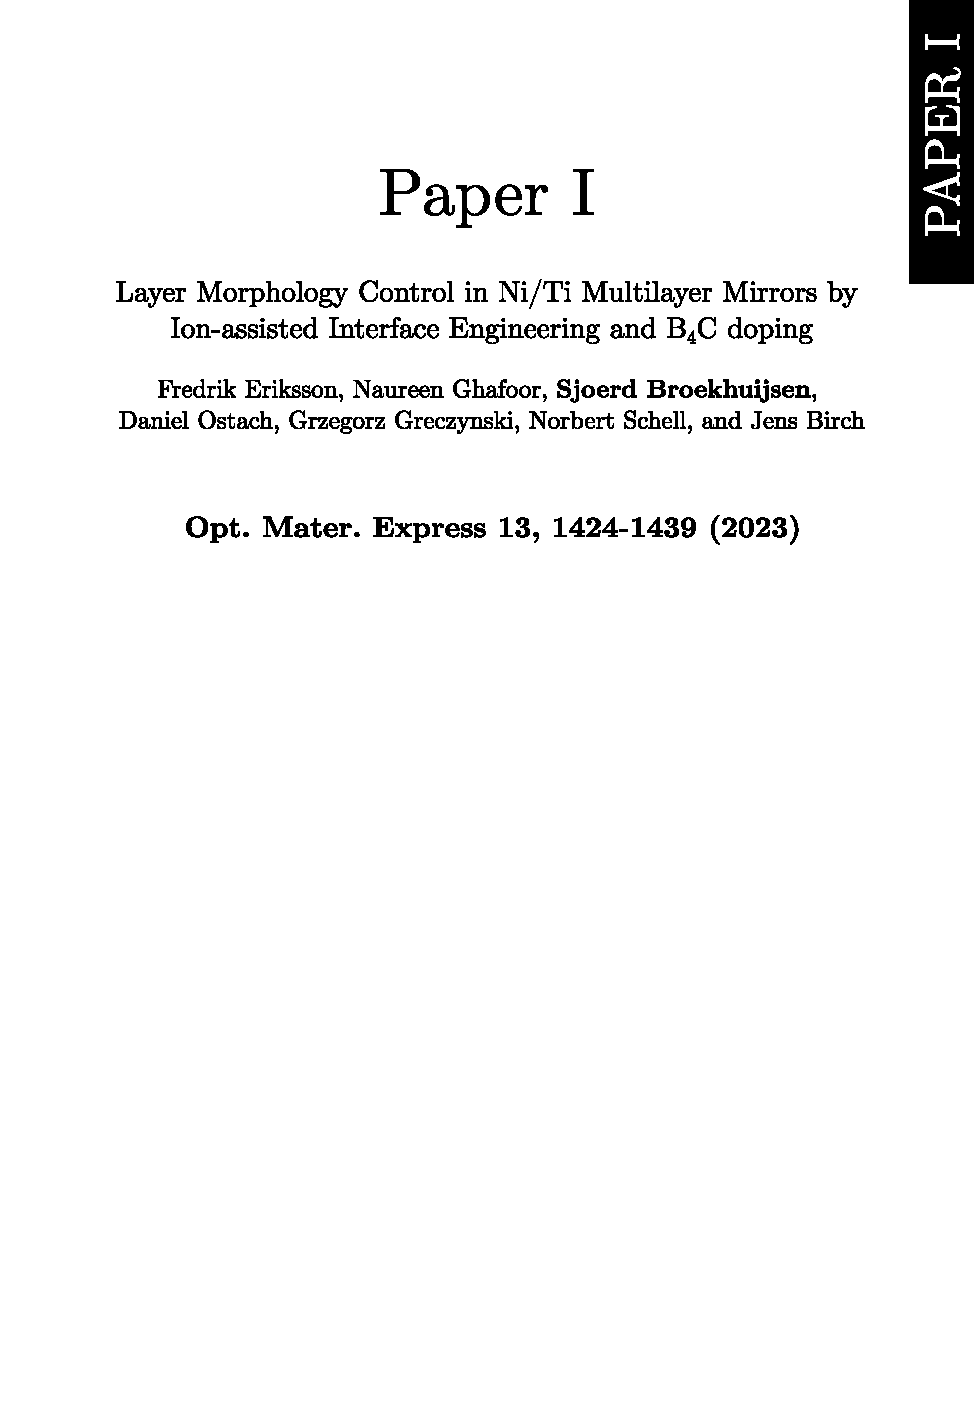
\includepdf[pages=-, width=\paperwidth, offset=-0.5cm 0cm]{paper1intro.pdf}

\includepdf[pages=-]{emptypage.pdf}
\includepdf[pages=-, width=\paperwidth]{article1.pdf}
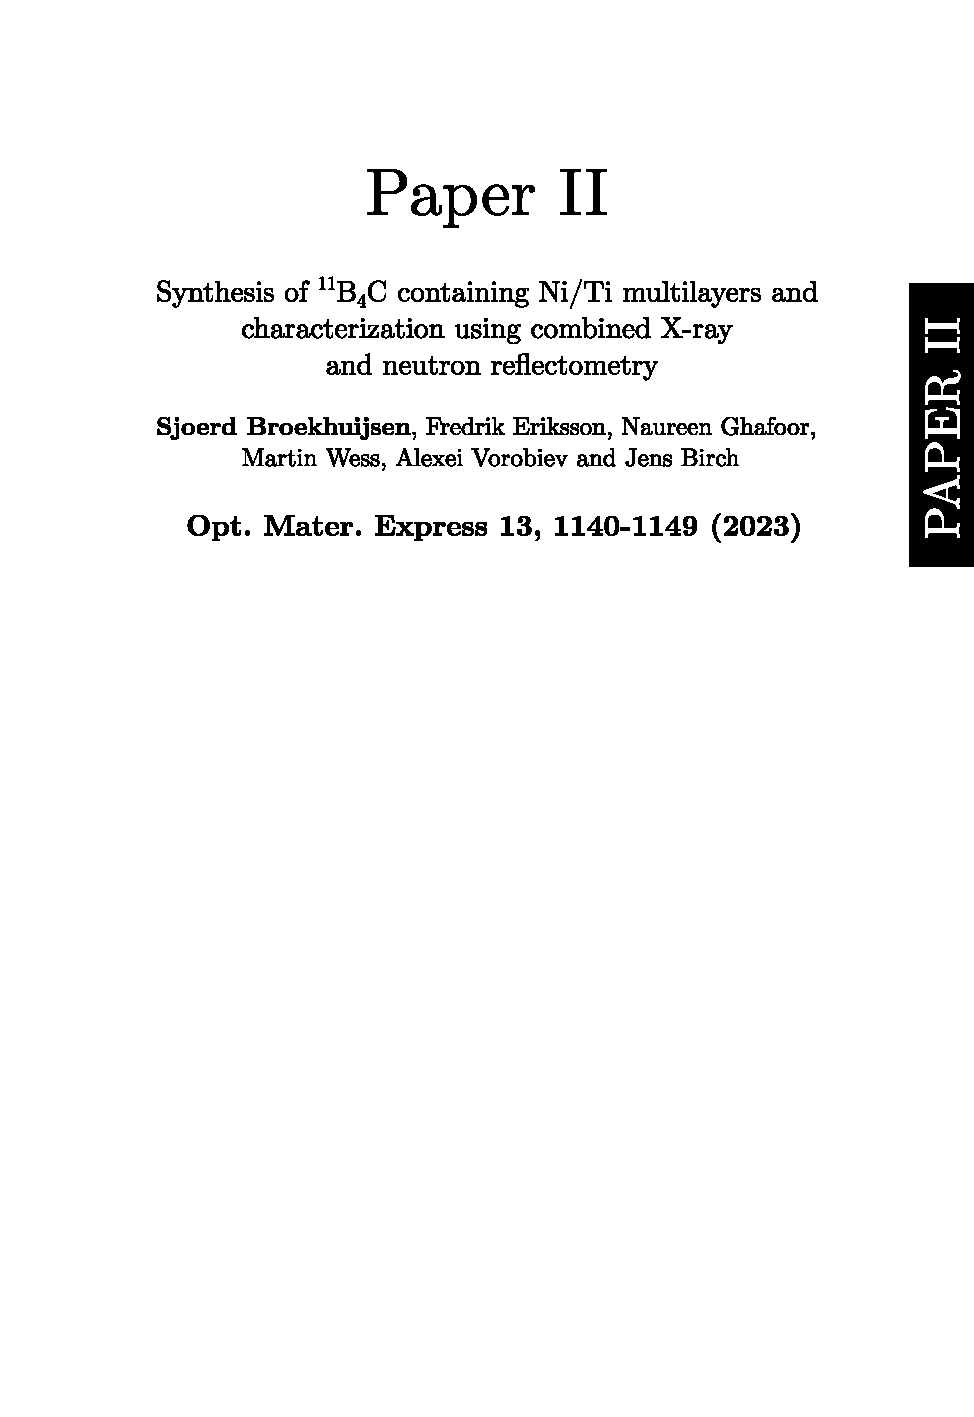
\includepdf[pages=-, width=\paperwidth, offset=-0.5cm 0cm]{paper2intro.pdf}

\includepdf[pages=-]{emptypage.pdf}
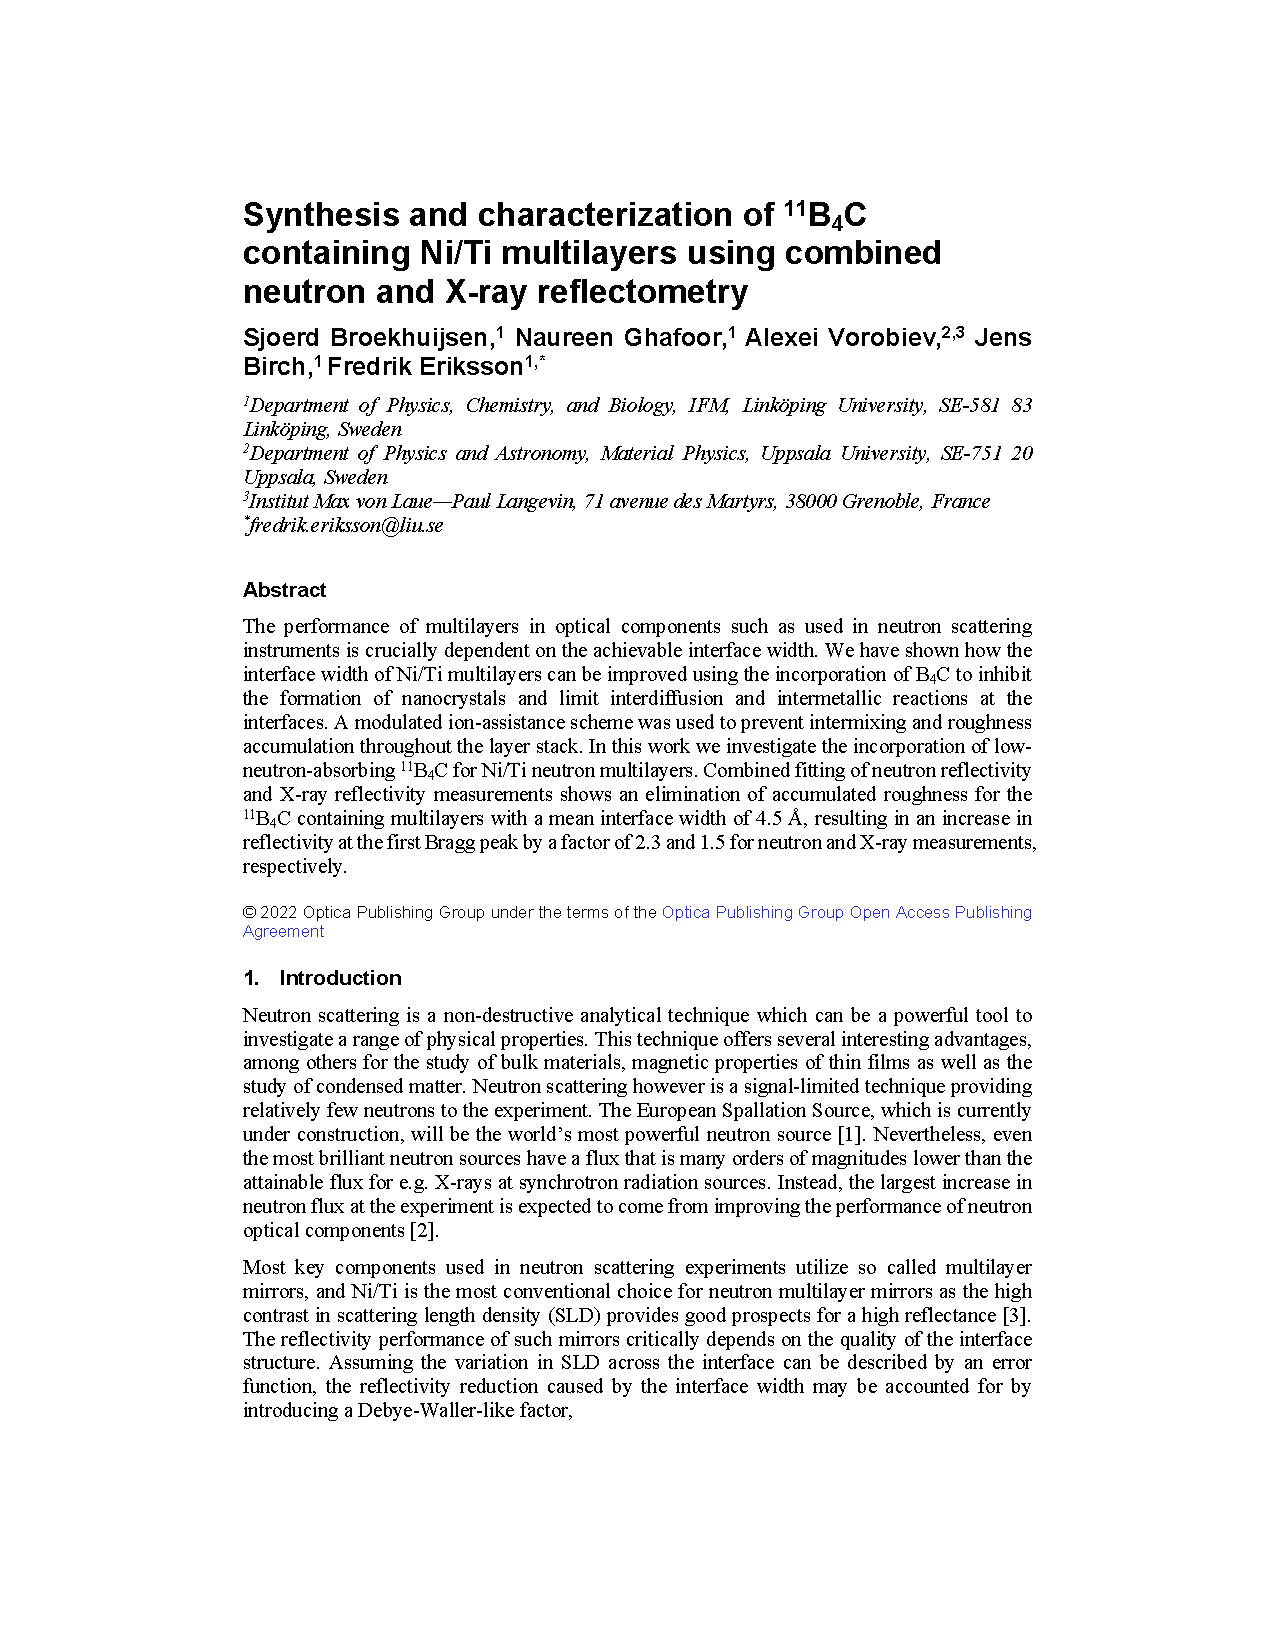
\includepdf[pages=-, width=\paperwidth]{article2.pdf}
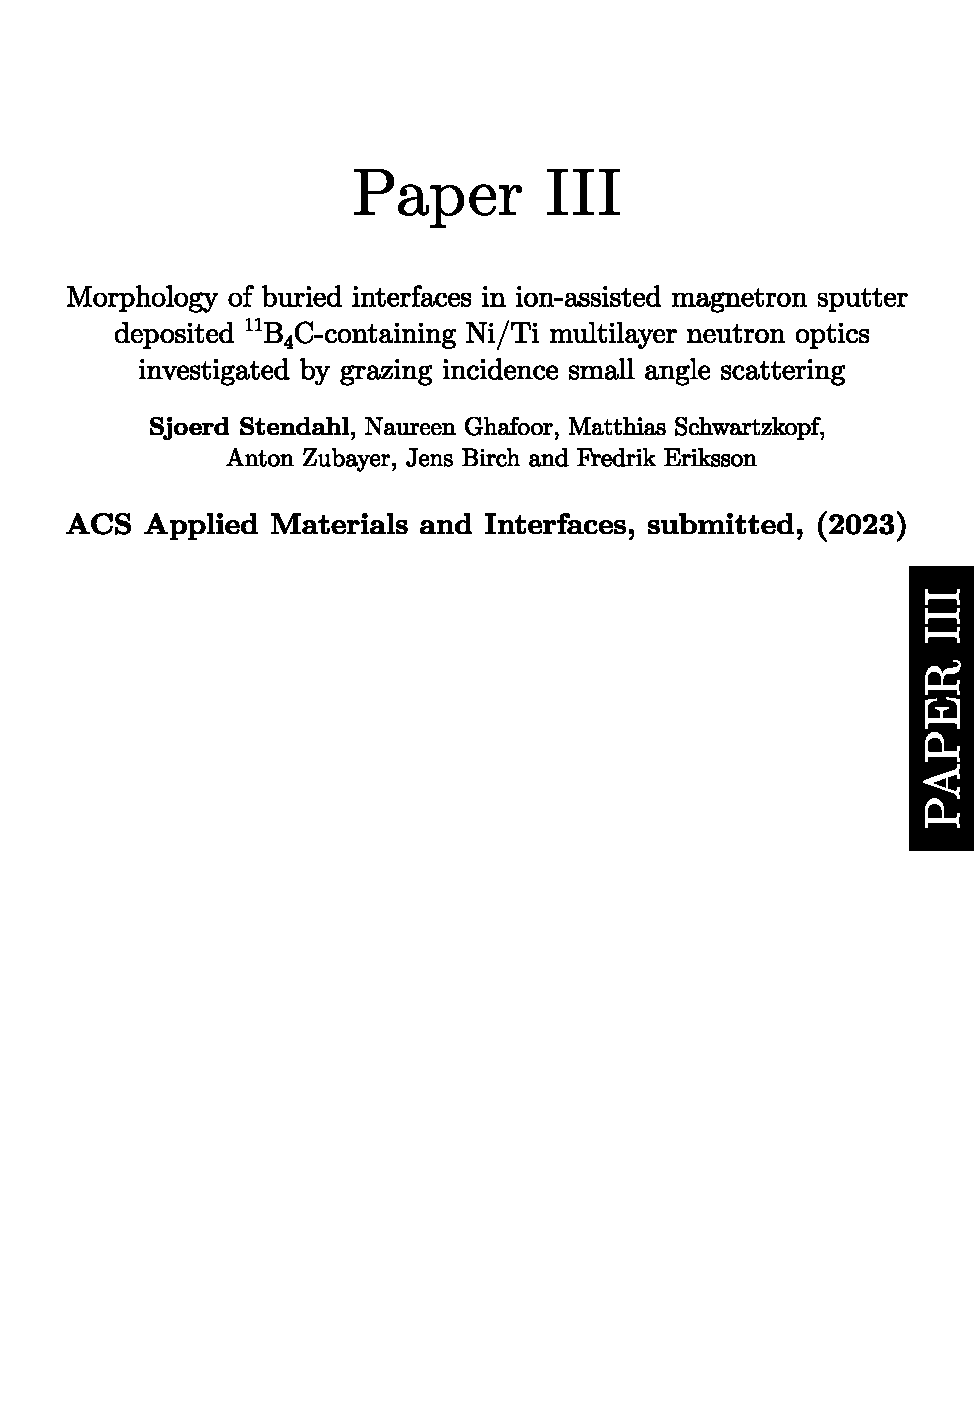
\includepdf[pages=-, width=\paperwidth, offset=-0.5cm 0cm]{paper3intro.pdf}

\includepdf[pages=-, width=\paperwidth]{emptypage.pdf}
%\includepdf[pages=-, width=\paperwidth]{article3.pdf}
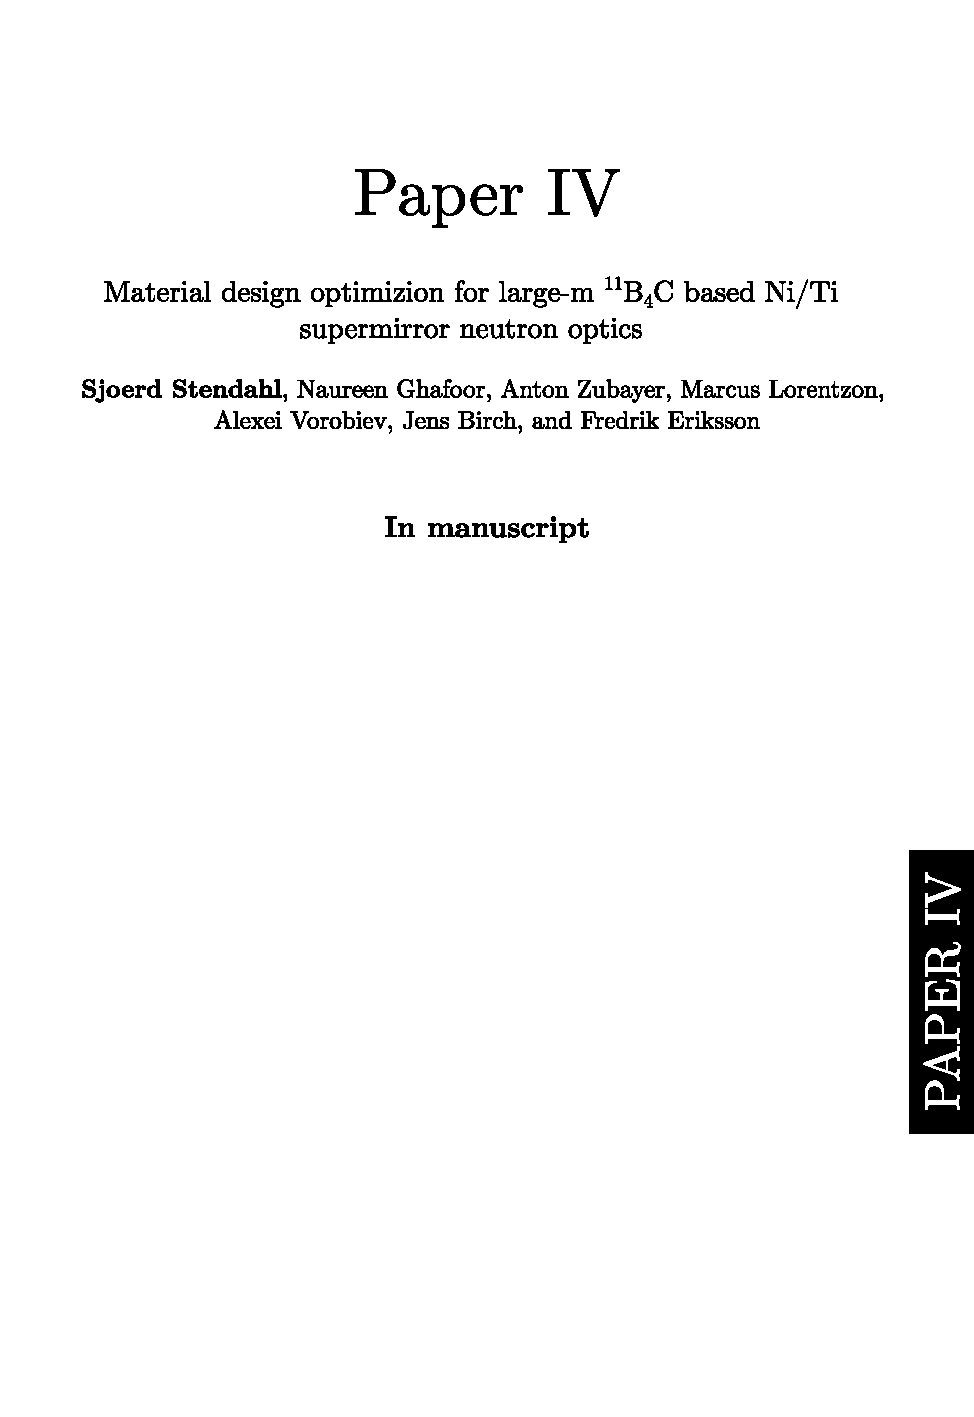
\includepdf[pages=-, width=\paperwidth, offset=-0.5cm 0cm]{paper4intro.pdf}
%\includepdf[pages=-, width=\paperwidth]{article4.pdf}

\includepdf[pages=-, width=\paperwidth]{emptypage.pdf}
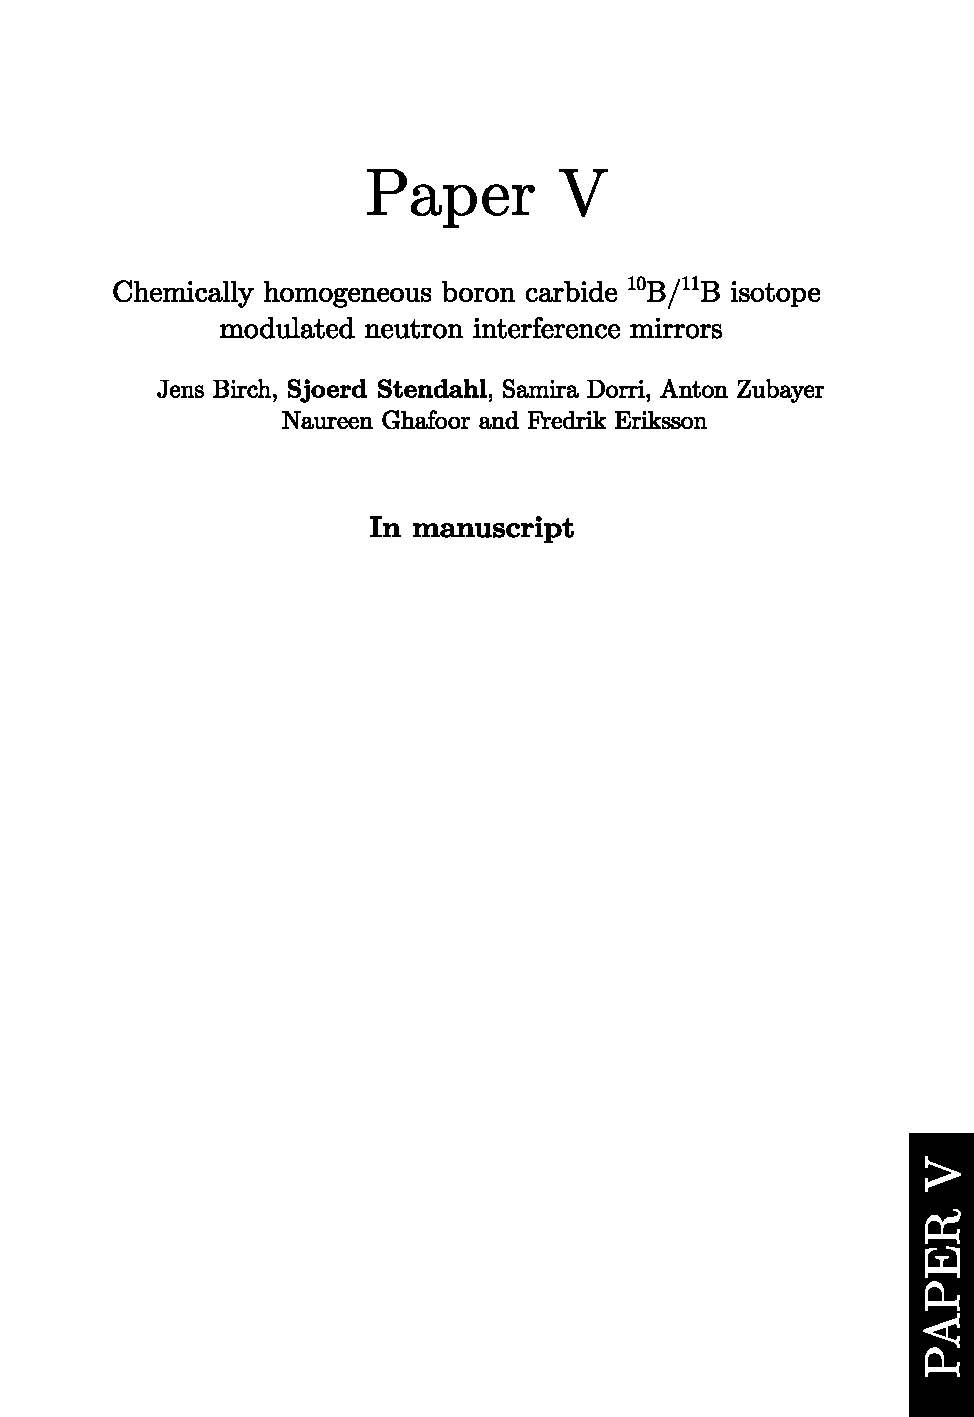
\includepdf[pages=-, width=\paperwidth, offset=-0.5cm 0cm]{paper5intro.pdf}

\includepdf[pages=-, width=\paperwidth]{emptypage.pdf}
%\includepdf[pages=-, width=\paperwidth]{article5.pdf}

\includepdf[pages=-, width=\paperwidth]{emptypage.pdf}
    \includepdf[pages=134, fitpaper=true]{FULLTEXT01.pdf}
\end{document}